\documentclass[12pt, a4paper, twoside]{book}

\title{Computable characterisations of stochastic uncertainty in dynamical systems}
\author{Liam Blake}
\date{\today}
\def\degree{Master of Philosophy}
\def\discipline{Applied Mathematics}


\usepackage{thesis}

% % Big line spacing
% \linespread{1.5}

% % Line numbering
% \RequirePackage{lineno}
% \linenumbers

\begin{document}
\frontmatter

\maketitle

% List of todos. Ugly but need to get them done!
\listoftodos

% Make the following tables
\tableofcontents
% \listoftables
\listoffigures

\chapter{List of Acronyms}
\newcommand{\acr}[2]{\item[] \textbf{#1:} #2}
\begin{itemize}
	\acr{ODE}{ordinary differential equation}
	\acr{SDE}{stochastic differential equation}
	\acr{PDF}{probability density function}
	\acr{FP}{Fokker-Planck}
	\acr{DA}{data assimilation}
	\acr{LCS}{Lagrangian coherent structure}
	\acr{EM}{Euler-Maruyama}
	\acr{FTLE}{finite-time Lyapunov exponent}
\end{itemize}

% Frontmatter
%!TEX root = ../thesis.tex
\chapter{Abstract}
\small
Differential equations are used ubiquitously to predict and understand phenomena across many fields.
These models are inevitably subject to uncertainties arising from a range of sources, including measurement error, unresolved components, and resolution limitations.
Accounting for these uncertainties leads to better models, but this is analytically challenging and often requires computationally expensive Monte Carlo simulation.
In this thesis, we consider It\^o stochastic differential equations, which extend ordinary differential equations to include stochastic terms and provide a rich framework for explicitly parameterising uncertainties in the model.
We look to address the need for computationally efficient methods that characterise uncertainty without resorting to the alternative of bulk simulation.

We first build upon previous small-noise studies to provide an explicit bound for the error between stochastic differential equations and corresponding linearisations written in terms of a deterministic system.
Our framework accounts for non-autonomous coefficients, multiplicative noise, and uncertain initial conditions.
These linearisations are solvable and efficient to compute and so can serve as an approximate solution to the stochastic differential equation.
We demonstrate the predictive power of our bound on several toy examples, providing for the first time a numerical validation of linearisation approximations of stochastic differential equations.
In characterising this relationship, we are also able to extend stochastic sensitivity (Balasuriya, \emph{SIAM Review}, 2020:781-816), a recently introduced tool for characterising the impact of uncertainty on differential equation solutions.
Stochastic sensitivity was previously restricted to 2-dimensional flows and we overcome this limitation to empower the use of these tools on models of arbitrary dimension.

We also propose an \emph{ad hoc} algorithm for approximating a stochastic differential equation solution with a Gaussian mixture model constructed from many different linearisations.
Such an algorithm is computationally efficient and provides an analytic probability density function, unlike stochastic samples.
Critically, the algorithm can capture non-Gaussian features in the stochastic solution that a single linearisation cannot.
Our initial investigation into this algorithm, using a data-driven model of a drifter in the Gulf Stream, yielded promising results to motivate future development.

Our work provides many avenues for further development, some of which we discuss briefly.
This includes theoretical extension to a broader range of stochastic models driven by different types of noise and implications for the Fokker-Planck equation, an equivalent representation of a stochastic differential equation.
We also anticipate applications within the fields of data assimilation, stochastic parameterisation, and, through a connection with results for discrete stochastic systems, mathematical epidemiology.

%!TEX root = ../thesis.tex
\chapter{Signed Statement}
 {\parindent=0pt\parskip=4ex

  %
  %  Check the University website for the current statements.  The ones below are from
  %    http://calendar.adelaide.edu.au/aprhdr/2016/specifications-thesis
  %  and valid for 2016
  %
  %  The second one is for when you are using material that is already published.
  %


  %4.1	For a thesis that does not contain work already in the public domain.

  I certify that this work contains no material which has been accepted for the award of any other degree or diploma in my name in any university or other tertiary institution and, to the best of my knowledge and belief, contains no material previously published or written by another person, except where due reference has been made in the text. In addition, I certify that no part of this work will, in the future, be used in a submission in my name for any other degree or diploma in any university or other tertiary institution without the prior approval of the University of Adelaide and where applicable, any partner institution responsible for the joint award of this degree.

  I give consent to this copy of my thesis, when deposited in the University Library, being made available for loan and photocopying, subject to the provisions of the Copyright Act 1968.

  I also give permission for the digital version of my thesis to be made available on the web, via the University's digital research repository, the Library Search and also through web search engines, unless permission has been granted by the University to restrict access for a period of time.

  %
  %%4.2	For a thesis that contains publications.
  %
  % 	I certify that this work contains no material which has been accepted for the award of any other degree or diploma in my name in any university or other tertiary institution and, to the best of my knowledge and belief, contains no material previously published or written by another person, except where due reference has been made in the text. In addition, I certify that no part of this work will, in the future, be used in a submission in my name for any other degree or diploma in any university or other tertiary institution without the prior approval of the University of Adelaide and where applicable, any partner institution responsible for the joint award of this degree.
  %
  %I give consent to this copy of my thesis when deposited in the University Library, being made available for loan and photocopying, subject to the provisions of the Copyright Act 1968.

  %The author acknowledges that copyright of published works contained within this thesis resides with the copyright holder(s) of those works.
  %
  %I also give permission for the digital version of my thesis to be made available on the web, via the University's digital research repository, the Library %Search and also through web search engines, unless permission has been granted by the University to restrict access for a period of time.
  %

  Signed: \dotfill\quad
  Date: \dotfill

 }

%!TEX root = ../thesis.tex
\chapter{Acknowledgements}
\label{ch:acknowledgements}

% %!TEX root = ../thesis.tex
\chapter{Dedication}
\label{ch:dedication}



\mainmatter

% Chapters
%!TEX root = ../thesis.tex

\chapter{Introduction}
%%% This is just a dump of the introduction to paper, comments and all.
\td{Make this introduction more general, less fancy words}
Many phenomena across geophysical, biological and socio-economic applications can be modelled using a continuous-time dynamical system, i.e., an ordinary differential equation \cite[e.g.]{BrauerCastillo-Chavez_2012_MathematicalModelsPopulation,TelEtAl_2005_ChemicalBiologicalActivity,Wiggins_2005_DynamicalSystemsApproach}.
Given initial values of a multi-dimensional state variable, such equations can be solved numerically to predict the state at future times.
The governing dynamics may be specified using existing phenomenological models, but in modern applications these are usually supplemented or driven by observed data \cite{LawEtAl_2015_DataAssimilationMathematical,ReichCotter_2015_ProbabilisticForecastingBayesian}.
Standard examples include the modelling of weather using available data \cite{LawEtAl_2015_DataAssimilationMathematical,ReichCotter_2015_ProbabilisticForecastingBayesian}, and predicting concentrations of, for instance, temperature, pollutants or phytoplankton in the ocean using observed current velocity data \cite{AbascalEtAl_2009_ApplicationHFRadar,dOvidioEtAl_2010_FluidDynamicalNiches}.





%, as a scalar measure of uncertainty about any solution trajectory of the deterministic model.
% This also extends stochastic sensitivity as a means of Lagrangian coherent structure extraction to fluid flows of arbitrary dimension.
% Moreover, by additionally accounting for initial condition uncertainty, we are able to relate stochastic sensitivity to the finite-time Lyapunov exponent (FTLE) \cite{ShaddenEtAl_2005_DefinitionPropertiesLagrangian,YouLeung_2021_ComputingFiniteTime,GuoEtAl_2016_FiniteTimeLyapunovExponents,Balasuriya_2020_UncertaintyFinitetimeLyapunov}.


% \rev{Finally, \citet{Sanz-AlonsoStuart_2017_GaussianApproximationsSmall} only consider two forms of initial conditions to the stochastic differential equation -- fixed values and Gaussian distributions -- whereas we provide a more general framework.}

% In general, however, a rigorous justification (in the sense of a limit, say) of such Gaussian approximations is lacking \cite{Sanz-AlonsoStuart_2017_GaussianApproximationsSmall} when the SDE includes \emph{both} time-dependent coefficients and multiplicative noise.
% A natural theoretical approach in the limit of small noise is to use a linearisation process for the SDE, reducing the otherwise analytically intractable SDE to a solvable linear one.
% Within the perspective of determining an uncertainty distribution for a prediction, though, such a linearisation has not been rigorously justified \cite{Sanz-AlonsoStuart_2017_GaussianApproximationsSmall}.
% Other approaches first assume a Gaussian distribution (again, without justification), and obtain formal computations for its mean and covariance \cite{SarkkaSolin_2019_AppliedStochasticDifferential}.
% \sab{Perhaps make a direct quotation here about the fact that this is not justified}

% We remedy these issues in this paper by developing an exact expression for a stochastic process such that solutions to the noisy SDE converge to this process in a precise fashion in the limit of small noise: notably, the expectation of the $ r $th mean of the difference between these converges at a rate of the $ r $th power of the noise parameter for any finite time for all $ r \ge 1 $ (see \Cref{thm:main}).


% In this paper, we build upon this previous work to provide an \emph{explicit bound} (see \cref{eqn:main_ineq} in \Cref{thm:main}) on every moment of the distance between the solution of an SDE and that of a linearisation about a chosen deterministic trajectory.
% We consider a general class of multidimensional SDEs with fully non-autonomous terms and multiplicative noise, and an arbitrary random initial condition following a specified distribution.
% Our bound is written in terms of the scale of ongoing noise and the uncertainty in the initial condition.


% We focus our attention on the first-order series expansion -- that is, a linearisation -- since this is the highest-order such term with an analytical solution \cite{Blagoveshchenskii_1962_DiffusionProcessesDepending}.
% This aim is motivated by the need for computationally efficient uncertainty quantification in climate applications \cite{BernerEtAl_2017_StochasticParameterizationNew,LeutbecherEtAl_2017_StochasticRepresentationsModel,Palmer_2019_StochasticWeatherClimate}, and more broadly dynamical systems \cite{Balasuriya_2020_StochasticSensitivityComputable,KaszasHaller_2020_UniversalUpperEstimate,BranickiUda_2021_LagrangianUncertaintyQuantification}.
% We consider a framework in which the distribution of the initial condition is known, which is a situation that arises, for example, in data assimilation \cite{BudhirajaEtAl_2019_AssimilatingDataModels,Jazwinski_2014_StochasticProcessesFiltering,LawEtAl_2015_DataAssimilationMathematical,ReichCotter_2015_ProbabilisticForecastingBayesian}.


% % For instance, one can formally ``linearise'' the SDE in some sense to obtain a Gaussian density, and this approach is used in filtering theory \cite{Jazwinski_2014_StochasticProcessesFiltering}.
% % Other approaches first assume a Gaussian distribution and obtain computations for its mean and covariance \cite{SarkkaSolin_2019_AppliedStochasticDifferential,ArchambeauEtAl_2007_GaussianProcessApproximations}.
% % However, both approaches lack rigorous justification and a precise understanding of \emph{how} the Gaussian distribution arises from the nonlinear SDE.

% % \begin{itemize}
% %     % \item A linearisation approach is common to approximate an analytically intractable SDE with a solvable linear one. Cite some examples in the literature of where it is used .

% %     % \item Formal linearisations of stochastic differential equations have been studied in the context of small-noise series expansions \cite{Blagoveshchenskii_1962_DiffusionProcessesDepending} and using large deviations theory \cite{FreidlinWentzell_1998_RandomPerturbationsDynamical}.

% %     \item Sanz-Alonso and Stuart provide an explicit bound on the KL-divergence, etc. Limited models, etc. Multiplactive noise, only in terms of KL-divergence, etc.

% %     \item Here, we build upon this work by providing an explicit proof for a general class of SDEs with multiplicative noise, nonautonomous terms, providing a strong error bouud written explicitly in terms of bounding and Lipschitz. This provides conditions on the initialisation of the linearisation under which the solution to the SDE converges, in the sense of a small noise limit.
% %     We show that \emph{all} moments converge towards those of the linearised solution.

% %     \item We also highlight that in the special case of a fixed or Gaussian initial condition, our results reduce to those used in Gaussian approximations \cite{SarkkaSolin_2019_AppliedStochasticDifferential,ArchambeauEtAl_2007_GaussianProcessApproximations,Jazwinski_2014_StochasticProcessesFiltering}
% % \end{itemize}



% In particular, this work fits in with recent interest in stochastic parameterisation as a means to account for unresolved subgrid effects in climate modelling \cite{BernerEtAl_2017_StochasticParameterizationNew,LeutbecherEtAl_2017_StochasticRepresentationsModel,Palmer_2019_StochasticWeatherClimate}.
% In particular, the recent review \cite{LeutbecherEtAl_2017_StochasticRepresentationsModel} concludes, ``The aim of current and future developments in stochastic representations of model uncertainty is to develop schemes that are computationally highly efficient and contribute only moderately to the overall computational cost...''.
% This paper provides one method to convert a stochastic parameterisation (formulated as a SDE) to a computationally cheaper set of coupled ODEs for the mean and variance of an approximate Gaussian, together with a convergence proof and error estimates.

% % The Gaussian distribution arises as the solution to a formal linearisation of the SDE about a deterministic trajectory (in the absence of noise).
% % By bounding all raw moments of the difference between the SDE and the linearised solutions by the noise scale (see \Cref{thm:main}), we show that the stochastic deviation converges in distribution to a multivariate Gaussian random variable (see \Cref{thm:gauss_dist}).

% An important special case arises when the initial condition is fixed, or follows a specified Gaussian distribution.
% providing a computable Gaussian distribution that is consistent with approximations seen in other literature \cite{Sanz-AlonsoStuart_2017_GaussianApproximationsSmall,SarkkaSolin_2019_AppliedStochasticDifferential}, and in particular filtering theory \cite{Jazwinski_2014_StochasticProcessesFiltering}.
% The covariance matrix characterising this Gaussian can be explicitly written in terms of the flow map of the underlying deterministic system and the (potentially spatio-temporally varying) diffusion matrix, and is available even if the deterministic model is only available via data.
% The Gaussian distribution is consistent with that seen in other literature \cite{Jazwinski_2014_StochasticProcessesFiltering, Sanz-AlonsoStuart_2017_GaussianApproximationsSmall, SarkkaSolin_2019_AppliedStochasticDifferential}, while we additionally show convergence of \emph{all} the moments of the deviation distribution.
% The results hold independently of the initial condition and for all finite times; the uncertainty evolution of any deterministic trajectory with time is therefore encapsulated in our results.





% In the absence of any other understanding of these multitudinous issues, a well-established way of tackling such uncertainties in the model is to think of these as stochastic \cite{BernerEtAl_2017_StochasticParameterizationNew,Oksendal_2003_StochasticDifferentialEquations}.
% Running many realisations of stochastic perturbations to the deterministic model can generate statistics to improve predictions and estimate their associated uncertainties \cite[e.g.]{BadzaEtAl_2023_HowSensitiveAre,Collins_2007_EnsemblesProbabilitiesNew}.
% However, in practice a very large number of simulations is necessary to generate convergent statistics \cite{FepponLermusiaux_2018_DynamicallyOrthogonalNumerical, Leutbecher_2019_EnsembleSizeHow}.
% Thus, numerically solving such stochastic systems -- potentially with data-based terms -- is often computationally expensive, and does not necessarily provide conceptual insight into how the model uncertainties affect predictions.
% Clearly, possessing a broader theoretical understanding of how stochastic terms impact continuous dynamical systems would be valuable.
% Often, the uncertainty in a system is expected to be small, but can have a significant impact on predictions from the model and must therefore be accounted for.


% In particular, \citet{Balasuriya_2020_StochasticSensitivityComputable} derived the limiting mean and variance of the noise-scaled deviation, and provided computable expressions in terms of the deterministic flow map and velocity field.
% However, this was restricted to two-dimensional systems and did not characterise the limiting distribution itself.


% {For discussion, my opinions: \\
% 1. Perhaps less focus on DA, stochastic parametrisation as the primary motivators for the paper. These are applications down-the-line but not the main target of this paper. \\
% 2a. I think stochastic sensitivity should come up earlier. "\cite{Balasuriya_2020_StochasticSensitivityComputable} derived the mean and covariance of a mathematical construct, albeit in two physical dimensions only. This paper extends the calculation of SS to arbitrary dimensions and additionally proves that SS is Gaussian" is a nice sentence!\\
% 2b. Consider including something on the Fokker-Planck equation (FPE)---and impossibility of exact solution---and then on the alternatives: simulating SDEs many times or approximations. \\
% 3. Point 2 leads nicely into discussing linearisations. I think you have
% \begin{enumerate}[label=(\roman{*}), ref=(\roman{*})]
%  \item Jazwinski: gives the linearisation but as a Taylor series
%  \item Sanz-Alonso: provides an error bound for the linearisation in terms of the KL divergence, but for additive noise
%  \item Sarkka: \cite[\S5.5]{SarkkaSolin_2019_AppliedStochasticDifferential} gives a general expression for all moments of the sde solution, but one that requires the exact solution to the FPE. \cite[9.1]{SarkkaSolin_2019_AppliedStochasticDifferential} then discusses a \emph{Gaussian assumed density approximation}, that allows calculation of the moments of the sde, but without rigorous justification.
% \end{enumerate}
% }


% \td{Shorten significantly, only mention contributions once}
% The contributions of this work are:
% \begin{itemize}
%     \item In \Cref{thm:main}, we provide an explicit bound on the strong error between a stochastic differential equation and an appropriate linearisation, capturing the impact of \emph{both} the ongoing linearisation and the choice of initial condition.
%     This builds upon previous studies of small-noise expansions \cite[e.g.]{Sanz-AlonsoStuart_2017_GaussianApproximationsSmall,Blagoveshchenskii_1962_DiffusionProcessesDepending,FreidlinWentzell_1998_RandomPerturbationsDynamical}, providing an direct proof in the multidimensional, fully-nonautonomous and multiplicative noise case, and an explicit expression for the bound while additionally extending these results to arbitrary initial conditions.
%     Using this bound, we provide conditions for the initialisation of the linearised equation.


%     % Be clear here. Two sentences - often lacks justification, OR when the justification is there, only additive or autonomous. "Albeit"
%     % The Gaussian distribution solving the linearised SDE appears in other literature and applications but often lacks justification \cite{Jazwinski_2014_StochasticProcessesFiltering, SarkkaSolin_2019_AppliedStochasticDifferential}.
%     % On the other hand, when the linearisation is justified, this is disregarding time-dependence in the coefficients and multiplicative noise \cite{Sanz-AlonsoStuart_2017_GaussianApproximationsSmall}.

%     \item We provide, in a single place, a framework for characterising uncertainty in a system of ordinary differential equations via now justified linearisations, whereas previously these results were placed across \lb{I have not quite worded this the way I would like; }
%     The solution of the linearisation is expressed as an independent sum of the transformed initial condition and the ongoing
%     In \Cref{thm:limit_moments}, the mean and covariance of the linearisation are written in terms of the diffusion term and gradients of \emph{either} the drift term (as a pair of ordinary differential equations consistent with that arising elsewhere \cite[e.g.]{Jazwinski_2014_StochasticProcessesFiltering, Sanz-AlonsoStuart_2017_GaussianApproximationsSmall, SarkkaSolin_2019_AppliedStochasticDifferential, ArchambeauEtAl_2007_GaussianProcessApproximations}, or the flow map of the corresponding deterministic system.
%     The latter is an alternative characterisation that allows the Gaussian distribution to be computed \emph{entirely from the solution dynamics} of a deterministic model and specification of any multiplicative noise effects known prior.

%     \item In \Cref{sec:theory_s2},

%     \item In \Cref{sec:numerics}, we validate the results of \Cref{sec:theory} using stochastic simulations from a 2-dimensional model.
%     In particular, we demonstrate that the first four moments of the distance between the realisations and the Gaussian limit follow the predicted bound.
%     We also illustrate a key prediction from \Cref{sec:theory_s2}; that the computable covariance matrix of the Gaussian limit captures the time-evolution of uncertainty, even when the noise is multiplicative.

% \end{itemize}

% In full, we therefore present a framework for ascribing uncertainty distributions to solutions of a deterministic model, characterised \emph{entirely from the solution dynamics} of the model and specification of any multiplicative noise effects known \emph{a priori}.
% The Gaussian distribution is rigorously established as a small noise limit, and serves as both an intrinsic characterisation of the impact of model dynamics on uncertainty, and as an approximate SDE solution.
% By accounting for multiplicative noise, the framework can capture any non-uniform uncertainty known prior.\jm{This feels like the third time the result is discussed in detail. I appreciate the slow build up, but can/should we shorten?}
% Discuss stochastic parameterisation here. Start with "Since this work is fundamental, we do not explicitly consider the parameters. However, the hope is that the work can aide the analysis of parameterisations or provide computationally efficient scheme.

% This work is relevant to the well-known ``stochastic parameterisation'' approach in weather and climate modelling, in which stochastic components are introduced to account for unresolved subgrid effects \cite{BernerEtAl_2017_StochasticParameterizationNew,LeutbecherEtAl_2017_StochasticRepresentationsModel,Palmer_2019_StochasticWeatherClimate}.
% Since this work is fundamental, in establishing a convergence result for a general class of stochastic differential equations, we do not explicitly describe how to construct an appropriate stochastic parameterisation (e.g. specification of the coefficients of the SDE).
% Instead, we expect that this convergence result will be useful in the analysis of stochastic parameterisations, and to convert otherwise computationally expensive schemes into an efficient approximations, a goal explicitly identified in \cite{LeutbecherEtAl_2017_StochasticRepresentationsModel}.
% We also expect that this work will find application in data assimilation \cite{BudhirajaEtAl_2019_AssimilatingDataModels,Jazwinski_2014_StochasticProcessesFiltering,LawEtAl_2015_DataAssimilationMathematical,ReichCotter_2015_ProbabilisticForecastingBayesian}, as a means of accounting for linearisation error and forecast uncertainty.
% The original stochastic sensitivity tools have been applied to identify Lagrangian coherent structures (LCSs) in 2-dimensional fluid flow \cite{BadzaEtAl_2023_HowSensitiveAre, Balasuriya_2020_StochasticSensitivityComputable}.
% By extending the theory of these tools into arbitrary dimensions, our results can also be used to extract coherent structures in \(n\)-dimensional flows.

% \section{Stochastic parameterisation}\label{sec:stoch_param}

In any modelling scenario, there will inevitably be uncertainty in the model specification. o
The possible sources of uncertainty include, but are not limited to:
\begin{itemize}
	\item missing processes
	\item the model is sourced from measured data, which itself includes observational error.
	\item
\end{itemize}



All methods using this approach have uncertainties in the model specification arising from a variety of sources \cite{FangEtAl_2020_DisentanglingResolutionPrecision}: the model not capturing all phenomena because of the inevitable lack of a complete understanding of all processes involved, errors in measured data, information only available on spatio-temporal grids (resolution error), etc.
There are generally two manifestations of this uncertainty: in the initial state, and in the ongoing evolution of the model itself.




Many numerical weather and climate prediction models rely upon a spatial discretisation for tractable analysis and simulation.
Often, an extremely high resolution is needed to produce accurate simulations and predictions; for example, \citet{DawsonEtAl_2012_SimulatingRegimeStructures} demonstrated such requirements\lb{Read paper and be specific about numbers} for the state-of-the-art European Centre for Medium-Range Weather Forecasts (ECMWF) forecast model.

\begin{figure}
	\begin{center}
		\begin{tikzpicture}[scale=1.5]
			\pgfdeclareimage{img}{chp01_introduction/figures/gulf_stream_ssh.pdf}

			\node at (4,3) {\pgfuseimage{img}};

			\foreach \x in {0,2,4,6,8}
			\foreach \y in {0,2,4,6}
				{
					\draw[->,color=red] (\x,\y) -- ++(rnd*360:rnd+0.2);
					\fill (\x,\y) circle (1.5pt);
				}
		\end{tikzpicture}
		\caption{An illustration of unresolved subgrid effects in a spatial discretisation.
			When a system is discretised, either from measurements or to numerically solve a model, processes between the grid points and no longer resolved or observed and yet can have a noticeable impact on the system.}
		\label{fig:subgrid_effects}
	\end{center}
\end{figure}




The formal introduction of stochastic terms to account for unknown and unresolved processes into an otherwise deterministic model is known as \emph{stochastic parameterisation}, particularly in scientific circles.
\citet{BernerEtAl_2017_StochasticParameterizationNew} review the need for stochastic parameterisation in weather and climate models and discuss how stochastic terms can quantify four different aspects of these models:
\begin{itemize}
	\item directly estimating uncertainty,
	\item reducing systematic model errors arising from unresolved subgrid processes,
	\item triggering regime changes, and
	\item encapsulating the effect of external forcing.
\end{itemize}
\citet{DawsonPalmer_2015_SimulatingWeatherRegimes} showed through simulation studies that the performance of a high-resolution purely deterministic model can be matched by a lower-resolution stochastic model.

Although stochastic parameterisation is more common in the atmospheric modelling context, oceanography also suffers from the same trade-off between spatial resolution and accuracy of predictions.
Consequently, there is much interest in emplying stochastic parameterisation in oceanographic modelling \citep{Griffa_1996_ApplicationsStochasticParticle}.
\td{Eddy parameterisation - turbulent flows are modelled as stochastic.}

The mathematical formulation of stochastic parameterisation -- where model predictions are now random quantities -- lends itself naturally to data assimilation \citep{BudhirajaEtAl_2019_AssimilatingDataModels,Jazwinski_2014_StochasticProcessesFiltering,LawEtAl_2015_DataAssimilationMathematical,ReichCotter_2015_ProbabilisticForecastingBayesian}, where ongoing observations are combined with predictions from a model to produce an improved forecast.
Data assimilation provides a framework that can simultaneously account for uncertainty in the observations and the model itself.
It has been shown that stochastic parameterisation can improve the quality of forecasts in data assimilation schemes \citep{MitchellGottwald_2012_DataAssimilationSlow,HaEtAl_2015_ComparisonModelError}, and so these applications are an active error of research \citep[e.g.]{GottwaldHarlim_2013_RoleAdditiveMultiplicative}.

\td{Flow from here into the need for maths - justifications, proofs, etc.?}
There is an emerging need to bridge the gap between mathematicians working on developing stochastic theory and algorithms, and the scientists looking to apply this work to their respective fields.
In particular, \citet{BernerEtAl_2017_StochasticParameterizationNew} conclude that ``geoscientists are often unaware of mathematically rigorous results that can aid in the development of physically relevant parameterizations, [while] mathematicians often do not know about open issues in scientific applications that might be mathematically tractable''.


Stochastic differential equations (SDEs) are a natural framework for introducing different sources of uncertainty into the continuous time evolution of a variable \citep{Oksendal_2003_StochasticDifferentialEquations,SarkkaSolin_2019_AppliedStochasticDifferential,KallianpurSundar_2014_StochasticAnalysisDiffusion}.
Generally, in modelling situations the dynamics are highly nonlinear and one expects the noise to vary with both time and state (i.e. the noise can be \emph{multiplicative}), e.g. in atmospheric \citep{SuraEtAl_2005_MultiplicativeNoiseNonGaussianity,Sura_2003_StochasticAnalysisSouthern} and oceanic \citep{KamenkovichEtAl_2015_PropertiesOriginsAnisotropic} systems and from experimental and observational considerations.
This complicates usage of the model for prediction and analysis; such SDEs are usually intractable to solve analytically and computationally expensive to approximate accurately.
Data-based models---that is, models possessing terms in the equations which are driven by data rather than by explicitly specified functions---and uncertainty in the initial state render additional problems in obtaining a theoretical understanding of the stochastic system.
Nonetheless, bulk stochastic simulation of these models is the gold standard in many applications, most notably climate modelling where large-scale ensemble predictions are used \citep{Collins_2007_EnsemblesProbabilitiesNew,LeutbecherEtAl_2017_StochasticRepresentationsModel}.

However, the most significant drawback of bulk stochastic simulation is the computational load.
In general, a large number of samples is required for convergent statistics and accurate inference.
The recent review by \citet{LeutbecherEtAl_2017_StochasticRepresentationsModel} highlights the need to develop computationally efficient schemes for quantifying stochasticity in weather and climate forecast models.
In particular, the authors state that ```the aim of current and future developments in stochastic representations of model uncertainty is to develop schemes that are computationally highly efficient and contribute only moderately to the overall computational cost...''.


Returning to a mathematical perspective, we are given a possibly highly nonlinear SDE with non-trivial noise components
We cannot solve such equations analytically, and numerical simulation is computationally expensive.
The overall aim of this thesis is to address this problem, by developing characterisations of uncertainty and algorithms for approximating solution probability densities (as opposed to just generating samples) that are computationally efficient.
We aim to take advantage of the computational ease of generating solutions to a deterministic system (relative to taking many samples of a stochastic one).


A common approach to characterising and approximating the solution of nonlinear SDEs with small noise is via a ``linearisation'' through time about a single deterministic trajectory.
A linearised stochastic differential equation, obtained by truncating Taylor expansions of each coefficient \citep[e.g.]{Jazwinski_2014_StochasticProcessesFiltering,Blagoveshchenskii_1962_DiffusionProcessesDepending}, can be solved analytically and is accordingly used across a diversity of literature and applications \citep{Jazwinski_2014_StochasticProcessesFiltering,SarkkaSolin_2019_AppliedStochasticDifferential,KaszasHaller_2020_UniversalUpperEstimate,ArchambeauEtAl_2007_GaussianProcessApproximations,Sanz-AlonsoStuart_2017_GaussianApproximationsSmall,LawEtAl_2015_DataAssimilationMathematical,ReichCotter_2015_ProbabilisticForecastingBayesian,BudhirajaEtAl_2019_AssimilatingDataModels}.
However, often these linearisations are applied without rigorous justification and a clear understanding of \emph{how} the linearisation relates to the nonlinear SDE.
This is particularly the case when the noise is multiplicative, which is a situation that is often ignored but necessary in practice.
In addition, there is little understanding of the impact of the choice of initialisation of the deterministic trajectory on the validity of the linearisation.
Much is already known about these linearisations; classical results in the context of small-noise series expansions \citep{Blagoveshchenskii_1962_DiffusionProcessesDepending} and large deviations theory \citep{FreidlinWentzell_1998_RandomPerturbationsDynamical} show that the strong error between SDE solution with a fixed initial condition and that of an appropriate linearisation is bounded.
\citet{Sanz-AlonsoStuart_2017_GaussianApproximationsSmall} establish a strong result, bounding the Kullback-Leibler divergence between the solutions of autonomous SDEs with additive stationary noise and a linearised equivalent. Their result considers both an uncertain initial condition, and the evolving error due to the discrepancy between the models.

% In \cref{sec:theory}, we directly bound the expectation of all moments of the distance between the linearisation and the true solution of the stochastic differential equation.
% Our result extends the former convergence result of \citep{Sanz-AlonsoStuart_2017_GaussianApproximationsSmall} in three ways: we predict the scaling of all moments of the error, in the presence of multiplicative noise terms, and including time-dependent coefficients in the stochastic differential equations. We directly compare our results with those of \cite{Sanz-AlonsoStuart_2017_GaussianApproximationsSmall} in \cref{sec:comparison}.
% In \Cref{sec:numerics}, we show numerically that the scaling of the strong error predicted by \Cref{thm:main} matches our predictions on three example SDEs in \(1\)- and \(2\)-dimensions.
% We confirm the predicted scaling for four moments of the error.


% In particular, \citet{SuraEtAl_2005_MultiplicativeNoiseNonGaussianity} demonstrate that linear deterministic dynamics with multiplicative noise can be produce the non-Gaussian statistics that we observed in real systems.


% The mixing effect that these eddies have on the surrounding flow can be modelled with spatiotemporally-varying diffusion \citehere, which via the Fokker-Planck equation can be equivalently formulated as a stochastic differential equation with multiplicative noise.
% The Lagrangian trajectories, incorporating these unresolved eddy effects, are then modelled as solutions to the stochastic differential equation.
% Equivalently, through the Fokker-Planck equation we can consider the evolution of a passive tracer undergoing advection due to the deterministic drift and diffusion from both any natural diffusivity and the unresolved processes.
% The probability density function that solves the Fokker-Planck equation can be instead thought of as a time-varying density (with the appropriate normalisation) of the tracer.
% For instance, the Fokker-Planck equation has been used to model the transport of ??? with a stochastic framework \citehere.
% Hence, understanding the evolution of solutions to a stochastic differential equation is valuable in oceanography, as a means of quantifying both observational error and unresolved subgrid processes.


% There are several different methods for quantifying eddy diffusivity given either observed tracer data or a global ocean circulation model.

% The simplest notion of eddy diffusivity is a defined by






% A recent approach by \cite{YingEtAl_2019_BayesianInferenceOcean} uses Bayesian inference to estimate the eddy diffusivity tensor from observed Lagrangian tracer data, by numerically solving the Fokker-Planck equation to compute a likelihood function.


% In summary, stochastic parameterisation



% \section{Limitations of stochastic simulation and the need for further development}\label{sec:bkg_sim_limits}
% The introduction of stochastic terms complicates both the analytical treatment of the model.
% For example, we saw in \Cref{sec:sde_theory} that adding even additive and stationary\lb{Is this the right word?? I mean that \(\sigma\) is constant, with no time-dependency}\td{need to define additive versus multiplicative properly.} noise to an analytically solvable non-linear deterministic model can make exact solutions intractable.
% Thus, across many applications the state of the art approach is to generate samples of the stochastic model and perform statistical inference.
% For example, Monte-Carlo simulation is used across weather forecasting \citep{LeutbecherEtAl_2017_StochasticRepresentationsModel}, \td{something atmospheric} and \td{something oceanic}.

% However, the most significant drawback of bulk stochastic simulation is the computational load.
% In general, a large number of samples is required for convergent statistics and accurate inference, as discussed by \citet{Leutbecher_2019_EnsembleSizeHow}.
% For a complex model, the computational load of computing a single realisation

% The recent review by \citet{LeutbecherEtAl_2017_StochasticRepresentationsModel} highlights the need to develop computationally efficient schemes for quantifying stochasticity in weather and climate forecast models.


% \td{Show the plateauing out that I am observing empirically when using a KDE . . . some literature on this?? This is a huge point to make}
% For example, suppose that we intend on using the probabilistic forecast of our stochastic model in an inference scheme, such as in data assimilation in which model predictions are combined with ongoing observations to produce an improved forecast \cite[e.g.]{LawEtAl_2015_DataAssimilationMathematical,BudhirajaEtAl_2019_AssimilatingDataModels, ReichCotter_2015_ProbabilisticForecastingBayesian}.
% This requires a probability density function or similar for our forecast, but in generating samples we initially only have a collection of finite discrete points.


% The purpose of this example was to highlight the importance of accounting for measurement error and unresolved processes in a ; when the dynamics are complicated, then any uncertainty can have a significant impact on our inferences from the model, both quantitatively and qualitatively.



\section{Contributions of this thesis}
In \Cref{ch:background}, we provide a brief background on stochastic differential equations and the tools we will use.
The remainder of the thesis, and the contributions each chapter proivides, are as follows:
\td{The following is possibly too specific/technical for this introduction.}
\begin{itemize}
	\item In \Cref{ch:linear_theory}, we address a deficiency in the \emph{theory} of SDE linearisations. %by providing an explicit bound on the strong error between a stochastic differential equation and an appropriate linearisation, capturing the impact of \emph{both} the ongoing linearisation and the choice of initial condition.
	      The aim here is to provide a rigorously justified framework for computing efficient approximations of nonlinear stochastic differential equations, subject to arbitrary and random initial conditions.
	      Much of the content in this chapter and the following \Cref{ch:linear_numerics} has been submitted for review as a research article to \emph{Communications in Mathematical Sciences} \citep{BlakeEtAl_2023_ConvergenceStochasticDifferential}.
	      This chapter is the primary theoretical contribution of this thesis, and includes:

	      \begin{itemize}
		      \item We first build upon previous studies of small-noise expansions \cite[e.g.]{Sanz-AlonsoStuart_2017_GaussianApproximationsSmall,Blagoveshchenskii_1962_DiffusionProcessesDepending,FreidlinWentzell_1998_RandomPerturbationsDynamical} to provide an direct proof of a bound on the error between the solution to an SDE and a corresponding linearisation about a deterministic trajectory.
		            Our result holds for a multidimensional and fully-nonautonomous SDE with multiplicative noise subject to an arbitrary initial condition, and the bound itself is written explicitly in terms of the scales of the uncertainty in the initial condition and the ongoing noise.


		            % Be clear here. Two sentences - often lacks justification, OR when the justification is there, only additive or autonomous. "Albeit"
		            % The Gaussian distribution solving the linearised SDE appears in other literature and applications but often lacks justification \cite{Jazwinski_2014_StochasticProcessesFiltering, SarkkaSolin_2019_AppliedStochasticDifferential}.
		            % On the other hand, when the linearisation is justified, this is disregarding time-dependence in the coefficients and multiplicative noise \cite{Sanz-AlonsoStuart_2017_GaussianApproximationsSmall}.

		      \item By providing explicit solutions to the lienarised SDE, we provide in a single place a framework for efficiently computing the solution, enable efficient approximation and characterisation of the nonlinear SDE without resorting to bulk Monte-Carlo simulation.
		            Such an approximation used across a range of literature and applications \citep{Jazwinski_2014_StochasticProcessesFiltering,SarkkaSolin_2019_AppliedStochasticDifferential,KaszasHaller_2020_UniversalUpperEstimate,ArchambeauEtAl_2007_GaussianProcessApproximations,Sanz-AlonsoStuart_2017_GaussianApproximationsSmall,LawEtAl_2015_DataAssimilationMathematical,ReichCotter_2015_ProbabilisticForecastingBayesian,BudhirajaEtAl_2019_AssimilatingDataModels} but is dispersed across many different sources and often stated without an explicit justification.
		            By considering a general nonlinear SDE, we are able to provide a single framework for computing such approximations.
		            \td{Need to rework this dotpoint}

		            % The solution of the linearisation is expressed as an independent sum of the transformed initial condition and the ongoing
		            % In \Cref{thm:limit_moments}, the mean and covariance of the linearisation are written in terms of the diffusion term and gradients of \emph{either} the drift term (as a pair of ordinary differential equations consistent with that arising elsewhere \cite[e.g.]{Jazwinski_2014_StochasticProcessesFiltering, Sanz-AlonsoStuart_2017_GaussianApproximationsSmall, SarkkaSolin_2019_AppliedStochasticDifferential, ArchambeauEtAl_2007_GaussianProcessApproximations}), or the flow map of the corresponding deterministic system.
		            % The latter is an alternative characterisation that allows the Gaussian distribution to be computed \emph{entirely from the solution dynamics} of a deterministic model and specification of any multiplicative noise effects known prior.

		      \item In \Cref{sec:theory_s2}, we use the linearisation framework to extend the notion of ``stochastic sensitivity'' first introduced by \citet{Balasuriya_2020_StochasticSensitivityComputable}, which seeks to explicitly quantify the impact of vector field uncertainty on the solution trajectories of dynamical systems \citep{BranickiUda_2021_LagrangianUncertaintyQuantification,KaszasHaller_2020_UniversalUpperEstimate,BranickiUda_2023_PathBasedDivergenceRates,Balibrea-IniestaEtAl_2016_LagrangianDescriptorsStochastic}.
		            Whereas previously the definition of stochastic sensitivity was restricted to two-dimensions \citep{Balasuriya_2020_StochasticSensitivityComputable}, we provide a new definition in arbitrary dimensions and prove a convenient expression for computation.
		            This is the second significant theoretical contribution of this work, enabling this new tool to be applied to a much broader class of models.

	      \end{itemize}

	\item In \Cref{ch:linear_numerics}, we validate the results of \Cref{sec:theory} using stochastic simulations from a 2-dimensional model.
	      In particular, we demonstrate that the first four moments of the distance between the realisations and the Gaussian limit follow the predicted bound.
	      We also illustrate a key prediction from \Cref{sec:theory_s2}; that the computable covariance matrix of the Gaussian limit captures the time-evolution of uncertainty, even when the noise is multiplicative.

	\item In \Cref{ch:gmm}, we outline an algorithm that employs the linearisation approximation to construct a Gaussian mixture model for the solution to a stochastic differential equation, which can capture non-Gaussianity while still being efficient to compute.
	      The algorithm is preliminary, with several implementation details deliberately left vague and warranting further development.
	      However, we demonstrate the potential of such an approach on examples in the following chapter.

	\item In \Cref{ch:appls}, we apply the tools developed in \Cref{ch:linear_theory,ch:gmm} to two examples constructed from observed data: the position of a sea surface drifter and a 5-dimensional compartmental model for an outbreak of Ebola.
	      The latter example arises from a different context---stochastic models on a discrete state space---where linearised stochastic differential equations arise from large-population limits \citep{Kurtz_1970_SolutionsOrdinaryDifferential,Kurtz_1971_LimitTheoremsSequences}.
	      We explain how these results imply that the theory we develop for stochastic differential equations can be applied to these models, opening up a whole new range of applications, particularly in mathematical biology and epidemiology.

	\item In \Cref{ch:outlook}, we conclude this thesis by discussing the possible applications and future extensions of our work.
	      Since our theory is reasonably general, and we have only outlined a mixture model algorithm, there is much scope for theoretical extension, further numerical investigation, and application to a range of models.
	      In the final chapter, we briefly discuss many of these possible future directions.


\end{itemize}

% The second contribution of the paper is to % In the context of two-dimensional, unsteady fluid flow, stochastic sensitivity works with Eulerian velocity data as the underlying deterministic model, and seeks to quantify the uncertainty in an eventual Lagrangian trajectory location.
% This methodology was originally developed by Balasuriya \cite{Balasuriya_2020_StochasticSensitivityComputable} as a tool for determining Lagrangian coherent structures (LCS) \cite{BalasuriyaEtAl_2018_GeneralizedLagrangianCoherent,HadjighasemEtAl_2017_CriticalComparisonLagrangian} in fluid flows, in that clusters of trajectories which have small uncertainty may be thought of as more ``coherent'' than others.
% In \Cref{sec:theory_s2}, we generalise the (formerly two-dimensional) stochastic sensitivity to arbitrary dimensions by proving that the stochastic sensitivity can be computed as the largest eigenvalue of the covariance matrix of the solution to the linearised equation from \cref{sec:theory}.
% Our expressions extend \cite{Balasuriya_2020_StochasticSensitivityComputable} by empowering a rapid computation of stochastic sensitivity, as previously the computation required three integrals of particular rotations of the gradient of the flow map.
% We demonstrate this computation in \cref{sec:comput_s2}.

%!TEX root = ../thesis.tex

\chapter{Background}\label{ch:background}
We begin this thesis by introducing the required technical back, most notably defining the flow map of a deterministic system and building up to It\^o stochastic differential equations to incorporating uncertainty into these models.
Further details on the technical results and tools employed later are provided in \Cref{app:theory}.
The chapter is concluded by summarising stochastic sensitivity \citep{Balasuriya_2020_StochasticSensitivityComputable}, which provided initial tools for characterising uncertainty in a computationally efficient manner and was the primary motivation for this work.

% In this chapter, we first motivate the need for stochastic models with a simple example predicting the path of a drifter in the Gulf Stream.o

% Throughout, we will use an example of tracking a drifter in the Gulf Stream to illustrate the concepts introduced.
% We will return to this example in more detail, including applying our later developments, in \Cref{ch:appls}.

% We then briefly review the current literature on stochastic parameterisation, which is the introduction of stochastic terms into otherwise deterministic models, in the context of atmospheric modelling, oceanography and climate forecasting.
% Finally, we highlight the limitations of bulk stochastic simulation as a means of working with complicated stochastic models, both in terms of computational costs and accuracy.
% This suggests the need, across a variety of applications, for developing computationally efficient methods for approximating prediction distributions of such stochastic models, which this thesis aims to address.


\section{Notation}
We adopt several notational conventions throughout this thesis, which are summarised here.
The set of \(n \times m\) matrices with real-valued entries is denoted as \(\R^{n\times m}\).
% In general, the \(i\)th component of a vector \(x\) is denoted by \(x_{i}\), except where there is already a subscript, in which case we write \(x_t^{(i)}\) to denote the \(i\)th component of \(x_t\), for instance.
% For a matrix \(A\), \(\left[A\right]_{\cdot i}\) typically refers to the \(i\)th column, and \(\left[A\right]_{i\cdot}\) the \(i\) the row of \(A\).
The norm symbol \(\norm{\cdot}\) with no additional qualifiers denotes the standard Euclidean norm for a vector and the spectral (operator) norm induced by the Euclidean norm, i.e.\ for an \(n \times n\) matrix \(A\)
\[
	\norm{A} = \sup\left\{\frac{\norm{Av}}{\norm{v}}\,\middle|\,v \in \R^n, \, \norm{v} \neq 0\right\}.
\]
For a random variable \(X\), we use \(\avg{X}\) to denote the expectation of \(X\) and \(\var{X}\) to denote the variance.
For a \(n\)-dimensional vector-valued random variable \(Y\), \(\avg{Y}\) again denotes the (now vector-valued) expectation of \(Y\), and \(\var{Y}\) denotes the covariance matrix of \(Y\).
That is, \(\var{Y}\) is the symmetric \(n\times n\) matrix with \((i,j)\)th component
\[
	\left[\var{Y}\right]_{ij} = \avg{Y_iY_j} - \avg{Y_i}\avg{Y_j} = \cov{Y_i, Y_j} = \begin{cases}
		\var{Y_i},      & \text{if } i = j, \\
		\cov{Y_i, Y_j}, & \text{otherwise},
	\end{cases}
\]
where
\[
	\cov{Y_i, Y_j} = \avg{\left(Y_i - \avg{Y_i}\right)\left(Y_j - \avg{Y_j}\right)}
\]
denotes the (scalar) covariance between \(Y_i\) and \(Y_j\).

\begin{figure}
	\begin{center}
		\begin{tikzpicture}
			\node (as) [draw] {Convergence almost surely};
			\node (p) [draw, below=of as] {Convergence in probability};
			\node (rm) [draw, right=of p] {Convergence in \(r\)th mean, \(r > 0\)};
			\node (qm) [draw, above=of rm] {Convergence in \(q\)th mean, \(q > r\)};
			% \node (rmom) [draw, below=of rm] {Convergence of \(r\)th moment};
			\node (d) [draw, below=of p] {Convergence in distribution};
			\path[->,thick] (as) edge  (p)
			(p) edge  (d)
			(qm) edge (rm)
			(rm) edge (p);
			% (rm) edge (rmom);
		\end{tikzpicture}
		\caption{The strength of each notion of convergence for random variables, where each directed arrow corresponds to an implication.
			These results are stated and proven in \citet{Bremaud_2020_ProbabilityTheoryStochastic}, for instance.}
		\label{fig:rv_conv_impl}
	\end{center}
\end{figure}

There are several notions of convergence for a sequence of random variables, which we briefly recall here.
Consider a sequence of \(m\)-dimensional random vectors \(X_1, X_2,\dotsc\) and an \(m\)-dimensional random vector \(X\).
We say that:
\begin{itemize}
	\item The sequence \(X_1, X_2, \dotsc\) converges \emph{in distribution} to \(X\) if
	      \[
		      \lim_{n\to\infty}F_n\left(x\right) = F(x),
	      \]
	      where \(F_n\) is the cumulative distribution function for \(X_n\) and \(F\) is the cumulative distribution function for \(X\), for every point \(x \in \R^m\) where \(F\) is continuous.
	      If this is the case, we write
	      \[
		      X_n \xlongrightarrow[\text{distribution}]{} X, \quad \text{as } n \to \infty.
	      \]
	      Note that the limiting random vector \(X\) need not be defined on the same probability space as the terms in the sequence \(X_1, X_2, \dotsc\); convergence in distribution is the only notion of convergence for which this is the case.


	\item The sequence \(X_1, X_2, \dotsc\) converges \emph{in probability} to \(X\) if for every \(\delta > 0\)
	      \[
		      \lim_{n\to\infty}P\left(\norm{X_n - X} < \delta\right) = 0,
	      \]
	      in which case we write
	      \[
		      X_n \xlongrightarrow[\text{probability}]{} X, \quad \text{as } n \to \infty.
	      \]

	\item The sequence \(X_1, X_2, \dotsc\) converges \emph{almost surely} to \(X\) if
	      \[
		      P\left(\lim_{n \to \infty}X_n = X\right) = 1,
	      \]
	      in which case we write
	      \[
		      X_n \xlongrightarrow[\text{almost surely}]{} X, \quad \text{as } n \to \infty.
	      \]

	\item For \(r > 0\), the sequence \(X_1, X_2, \dotsc\) converges \emph{in \(r\)th mean} to \(X\) if
	      \[
		      \lim_{n\to\infty}{\avg{\norm{X_n - X}^r}} = 0,
	      \]
	      in which case we write
	      \[
		      X_n \xlongrightarrow[r\text{th mean}]{} X, \quad \text{as } n \to \infty.
	      \]
	      This type of convergence is also known as \emph{\(L_r\)-convergence}, as it corresponds to convergence in the \(L_r\) norm on the probability space on which \(X_1,\dotsc, X_n\) and \(X\) are defined.

\end{itemize}
There are implications between each notion of convergence, with convergence almost surely being the strongest and convergence in distribution the weakest.
These implications are summarised in \Cref{fig:rv_conv_impl}.

We often work with stochastic processes that evolve through time, for example, the Wiener process or the solution to a stochastic differential equation.
We generically use the notation \(y_t\), for instance, to denote the stochastic process, where \(t\) refers to time and \(y\) is a label.
The index set of the process is always a finite time interval, typically initialised at \(0\).
In almost all cases where we are working with \(y_t\) mathematically, \(y_t\) refers to the state of the process at the \emph{fixed} time \(t\).
When discussing a stochastic process in our prose, we also use \(y_t\) to refer to the \emph{full} solution path (where the possible values of \(t\) are known in context); this is an abuse of notation, but has no impact on the rigour of our mathematical results.




\section{The flow map}
Ordinary differential equations are used to model many different phenomena across a range of fields and applications.
Specifically, the continuous time evolution of a multi-dimensional state variable is governed by a system of first-order differential equations of the form
\begin{equation}\label{eqn:det_ode}
	\dod{w_t}{t} = u\!\left(w_t, t\right),
\end{equation}
where \(w_t \in \R^n\) is the time-evolving variable of interest and \(u\) is the vector field specified at each relevant state and time \(t\).
The vector field \(u\) may be derived from a specified model or may be driven or supplemented by observed data.
Since data has a finite-time limitation, we typically consider the evolution of \cref{eqn:det_ode} over a finite time interval \([0,T]\).
% In this thesis, we restrict ourselves to the finite time setting.
We can solve \cref{eqn:ode_det} analytically, or, as is often required in practice, numerically to generate trajectories, which can inform future predictions or be used to reconstruct past behaviour.
% The solutions to the differential equations of the form \cref{eqn:det_ode} define a continuous-time dynamical system.
The flow map of \cref{eqn:det_ode} provides a convenient way of summarising the trajectories that solve \cref{eqn:det_ode} and working with these solutions analytically.
Formally, the flow map \(F_{s}^{t}: \R^n \to \R^n\) from time \(s\) to \(t\) associated with \cref{eqn:det_ode} is the unique solution to
\begin{equation}
	\dpd{F_{s}^{\tau}\!\left(x\right)}{\tau} = u\left(F_{s}^\tau\!\left(x\right), \tau\right), \qquad F_{s}^{s}\!\left(x\right) = x,
	\label{eqn:flow_map_ode}
\end{equation}
solved up to time \(\tau = t\).
That is, the flow map is the operator mapping initial conditions at time \(t\) to their corresponding positions at time \(s\), under the continuous-time evolution of \cref{eqn:det_ode}.
Equivalently, the flow map satisfies the integral form of \cref{eqn:det_ode}:
\begin{equation*}
	F_s^t\!\left(x\right) = x + \int_s^t{u\!\left(F_s^{\tau}\!\left(x\right), \tau\right)\dif \tau}.
\end{equation*}
We use the flow map to represent all solutions of the deterministic differential equation \cref{eqn:det_ode}, understanding that for any relevant initial condition, the flow map at that point can be readily computed by solving the ODE either analytically or numerically.
For a well-defined flow, the flow map \(F_s^t\) is reversible, in that we could have \(t < s\), with the property
\[
	F_s^t\!\left(F_t^s\!\left(x\right)\right) = x,
\]
for any times \(s\) and \(t\).
We view the flow map primarily as a function of the initial condition, so that it quantifies the impact of changes in the initial condition on future predictions.
Accordingly, the gradient \(\nabla F_s^t\) of the flow map (with respect to the initial condition) provides insight into the local behaviour of the dynamical system \citep{Arnold_1973_OrdinaryDifferentialEquations,TruesdellNoll_2004_NonLinearFieldTheories}.
For any times \(s, t \in [0,T]\), this gradient	\(\nabla F_s^t\) satisfies a useful property:
\begin{equation}
	\dpd{\nabla F_{s}^{t}\!\left(x\right)}{t} = \nabla u\!\left(F_{s}^{t}\!\left(x\right), t\right) \nabla F_{s}^{t}\!\left(x\right),
	\label{eqn:eqn_of_variations}
\end{equation}
which is the equation of variations corresponding to \cref{eqn:det_ode}.
This result can be shown by taking the gradient of both sides in \cref{eqn:flow_map_ode} and using the chain rule.




\section{From ODEs to SDEs}
Differential equations are well-studied and ubiquitously employed across many fields.
These models are \emph{deterministic}, in that, given an initial condition, an ODE provides a single prediction of the future state.
However, as discussed in the introduction, any such model will be subject to unavoidable uncertainty, which can arise from a range of sources.
By accounting for any of these in our model, we expect to improve the power and accuracy of our predictions.
However, the true nature of this uncertainty is unknowable, so it is common to model it as a random process.
We extend our deterministic model to a \emph{stochastic} one, where the solution (and therefore our predictions of the future state) is now a random variable with a probability distribution defined over the state space.
There are several approaches to establishing such a framework, the most general of which is a random dynamical system \citep{Arnold_1998_RandomDynamicalSystems,NeckelRupp_2013_RandomDifferentialEquations}.
When working in a continuous-time and continuous-state modelling scenario, a natural extension of an ordinary differential equation to account for this uncertainty is a stochastic differential equation (SDE) \citep{Oksendal_2003_StochasticDifferentialEquations,KallianpurSundar_2014_StochasticAnalysisDiffusion}, where the uncertainty is modelled with an additional term.
Although an SDE is an ``improvement'' over the deterministic ODE, in the sense that uncertainty can be encoded in the model itself, the compromise is that solutions are no longer straightforward to obtain or even analyse.
In fact, the formal treatment of SDEs requires an entirely new notion of integration, as we shall discuss.
Nonetheless, SDEs provide a rich framework for modelling and are used as predictive tools in a range of applications and fields. % \citep{Balasuriya_2020_StochasticApproachesLagrangian,SarkkaSolin_2019_AppliedStochasticDifferential,Oksendal_2003_StochasticDifferentialEquations,Jazwinski_2014_StochasticProcessesFiltering}.
There are several distinct ways to construct stochastic differential equations from deterministic dynamics; the following motivation of stochastic differential equations loosely follows a similar one available in \citet{Oksendal_2003_StochasticDifferentialEquations}, but other formulations of SDEs are available, e.g.\ using rough path theory \citep{FrizVictoir_2010_MultidimensionalStochasticProcesses} or by averaging the `fast' dynamics in a multiscale system \citep{MelbourneStuart_2011_NoteDiffusionLimits,GottwaldMelbourne_2013_HomogenizationDeterministicMaps,PavliotisStuart_2008_MultiscaleMethods}.

Suppose that we have a deterministic ordinary differential equation, i.e.\ \cref{eqn:ode_det}, and aim to account for uncertainty in the vector field \(u\).
In lieu of any additional understanding of this uncertainty, we model it as a stochastic noise.
Ideally, we would parameterise the uncertainty with some continuous-time stochastic process \(\xi_t\), and write
\begin{equation}\label{eqn:fake_sde}
	\dod{y_t}{t} = u\left(x_t, t\right) + \sigma\!\left(x_t, t\right)\xi_t,
\end{equation}
where \(\sigma\) is a specified part of the model that modulates how the magnitude and structure of the uncertainty varies with state and time.
Since we are modelling with a continuum, the noise process \(\xi_t\) should be (with probability \(1\)) continuous in time, and should, with no additional prior knowledge, evolve independently of itself through time, follow a probability distribution that does not depend on time, and have zero expectation.
That is, \(xi_t\) should be a white noise process in the absence of any additional knowledge of the nature of the noise, beyond the specification of \(\sigma\).
However, there does not exist \emph{any} process \(x_t\) that satisfies all of these properties simultaneously \citep{Oksendal_2003_StochasticDifferentialEquations}; continuity cannot be enforced.
This complication requires an alternative formulation, which leads to an entirely new type of calculus built around the It\^o integral and It\^o stochastic differential equations, which we introduce in \Cref{sec:bkg_ito} and \Cref{sec:bkg_sde} respectively.

% In most modelling situations, we expect that the noise process \(\xi_t\) should have the properties:
% \begin{enumerate}
% 	\item For any two distinct times \(s \neq t\), the random variables \(\xi_s\) and \(\xi_t\) are independent.
% 	\item The process is stationary, that is the joint distribution of \(\xi_{t_1 + t}, \dotsc, \xi_{t_k + t}\) does not depend on \(t\).
% 	\item For all \(t\), \(\avg{\xi_t} = 0\).
% \end{enumerate}
% Additionally, since we are modelling with a continuum, the noise process \(\xi_t\) should be (with probability \(1\)) continuous in time.
% However, such a noise process \(\xi_t\) does not exist \citep{Oksendal_2003_StochasticDifferentialEquations}, in that there is no  continuous process with properties 1 to 3, so we need an alternative formulation of the integral.
% This leads to the It\^o integral, and It\^o stochastic differential equations, which we introduce in \Cref{sec:bkg_ito} and \Cref{sec:bkg_sde} respectively.

\subsection{The Wiener process}

\begin{figure}
	\begin{center}
		% 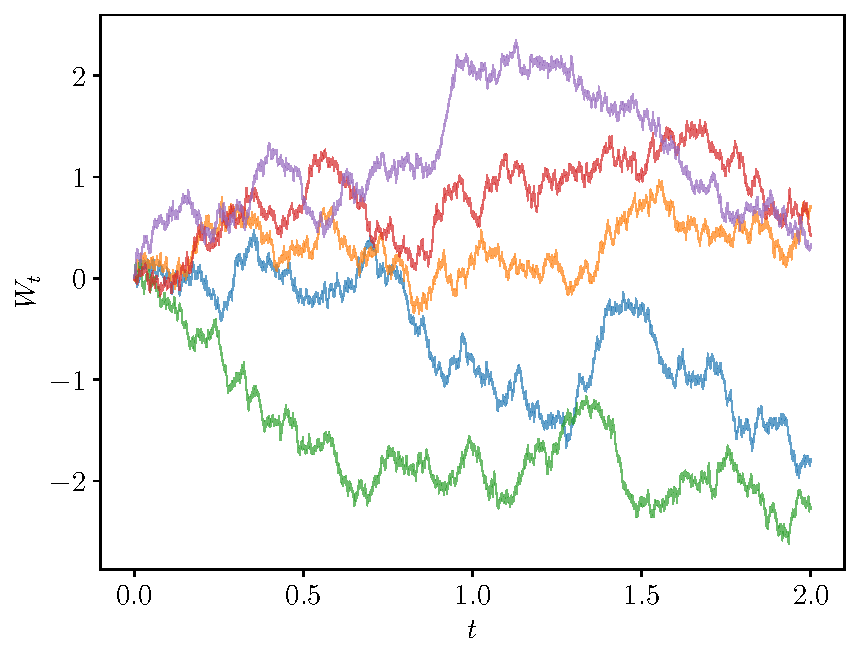
\includegraphics[width=0.49\textwidth]{chp02_background/figures/wiener_realisations_1d.pdf}
		% 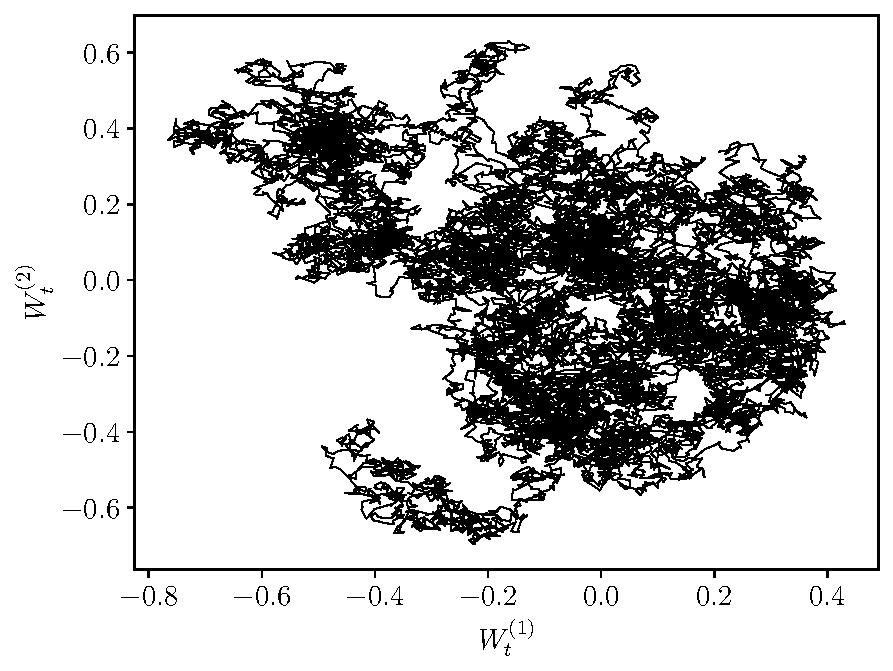
\includegraphics[width=0.49\textwidth]{chp02_background/figures/wiener_realisations_2d.pdf}
		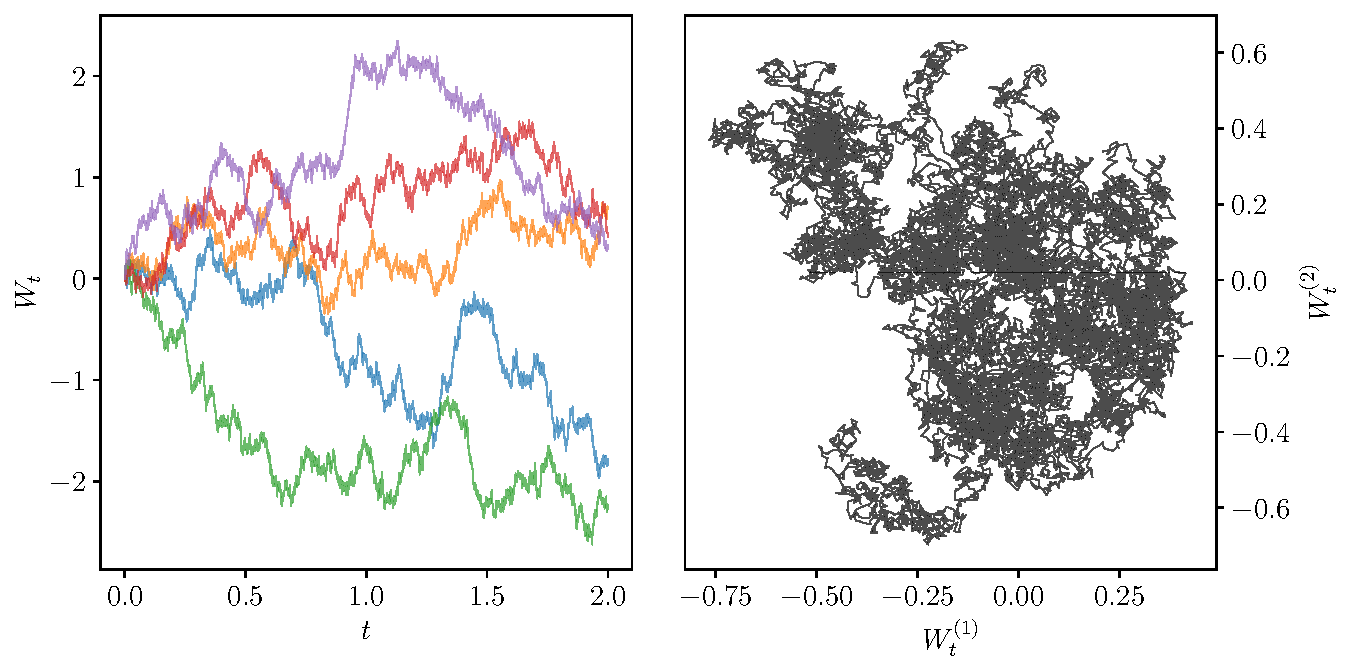
\includegraphics[width=\textwidth]{chp02_background/figures/wiener_realisations}
		\caption{(Left) Several realisations of a 1-dimensional Wiener process \(W_t\) evolving through time, and (right) a realisation of 2-dimensional Wiener process \(\left(W_t^{(1)}, W_t^{(2)}\right)^{\T}\).}
		\label{fig:wiener_rels}
	\end{center}
\end{figure}

In the absence of any additional knowledge about the noise (such as skew or heavy-tailedness), the canonical Wiener process is the standard choice as the driving stochastic process.
The Wiener process is the definite integral of a white noise process and is, therefore, an appropriate choice to ensure that the ``solution'' (the result after integration through time) of \cref{eqn:fake_sde} involves the idealised noise process \(\xi_t\) that we were initially after. %\lb{I don't think this makes any sense to the reader, but it's difficult to explain this intuitively. I believe that the idea is that this white noise process is the `derivative' of the Wiener process (in the sense that \(W_t\) is the integral of \(\xi_t\)).}.
Defined formally, the (1-dimensional) canonical \emph{Wiener process} is a stochastic process \(B_t\) that takes values in \(\R\) and satisfies the following properties \citep{KallianpurSundar_2014_StochasticAnalysisDiffusion}:
\begin{romanate}
	\item \(B_0 = 0\) almost surely,
	\item for every \(s > 0\), the increments \(B_{s + t} - B_{s}\) for \(t \geq 0\) are independent of \(B_r\) for all \(r < s\),
	\item \(B_{s + t} - B_t \isGauss{0, s}\) for all \(s,t > 0\), and
	\item \(B_t\) is continuous in \(t\) almost surely.
\end{romanate}
Remarkably, these properties \emph{uniquely} define the Wiener process, with the additional result that for any \(t > 0\), \(B_t\) is distributed as \(\mathcal{N}\left(0, t\right)\), a Gaussian distribution with mean zero and variance \(t\).
The \emph{\(n\)-dimensional Wiener process} is a stochastic process \(W_t\) that takes values in \(\R^n\) and is such that each component of \(W_t\) is a 1-dimensional Wiener process and the components of \(W_t\) are mutually independent.
It follows that for the \(n\)-dimensional Wiener process \(W_t\), at any time \(t > 0\), \(W_t \sim \mathcal{N}\left(0, tI\right)\), an \(n\)-dimensional Gaussian distribution with mean zero and covariance matrix \(tI\).
\Cref{fig:wiener_rels} plots realisations of a 1-dimensional and 2-dimensional Wiener process.

\subsection{The It\^o integral}\label{sec:bkg_ito}
With probability \(1\), the path of a Wiener process is continuous, but differentiable nowhere, so standard deterministic calculus is not sufficient to introduce continuous-time uncertainty into a differential equation.
Instead, this led to an entirely new definition of the integral by \citet{Ito_1944_StochasticIntegral,Ito_1946_StochasticIntegralEquation} that allowed integration with respect to a broad class of stochastic processes, laying the foundation for the formal framework of stochastic differential equations.
Here, we provide one definition of the It\^o integral but do not go into technical detail.
See the textbooks by \citet{KallianpurSundar_2014_StochasticAnalysisDiffusion} and \citet{Oksendal_2003_StochasticDifferentialEquations}, for instance, for a detailed introduction to and construction of the It\^o integral and subsequent properties.
We only consider integrals with respect to canonical Wiener processes, but generalisations of the driving process are possible \citep{Applebaum_2004_LevyProcessesStochastic}.
For our purposes, we can define an It\^o integral as the limit in probability of a sequence of sums: for a scalar but possibly random-valued function \(f\colon [a,b] \to \R\), the \emph{It\^o integral} of \(f\) with respect to the Wiener process \(W_t\) is the limit
\begin{equation*}\label{eqn:ito_int_limit_defn}
	\sum_{\left[t_i, t_{i+1}\right] \in \mathcal{P}_N}{f\left(t_{i}\right)\left(W_{t_{i+1}} - W_{t_i}\right)} \xlongrightarrow[\text{probability}]{} \int_a^b{f(t)\dif W_t}, \quad \text{as } N \to \infty
\end{equation*}
where \(\mathcal{P}_N\) is a partition of \(\left[a,b\right]\) with \(\lim_{N \to \infty}\mathcal{P}_N = [a,b]\), \emph{\`a la} the definition of the Riemann integral.
The It\^o integral is itself a random variable.
It can be shown \citep[e.g.]{KallianpurSundar_2014_StochasticAnalysisDiffusion,Oksendal_2003_StochasticDifferentialEquations} that this limit exists for a large class of both deterministic- and random-valued functions, by constructing appropriate approximations of the function \(f\).
There are several other definitions of the stochastic integral, the most common alternative being the Stratonovich integral \citep{Stratonovich_1966_NewRepresentationStochastic}, which results from a different interpretation of the noise term in \cref{eqn:fake_sde} and is often used in physics.
The Stratonovich integral in particular can be re-interpreted as an It\^o integral with an appropriate transformation of the integrand, so we focus our attention in this thesis solely on the It\^o formulation of stochastic calculus.
% Such functions for which the integral exist are termed \emph{It\^o-integrable} and are those that are measurable with respect to the probability space on which the Wiener process is defined
% \td{Should probably summarise what these functions look like}

The extension of the It\^o integral to vector- and matrix-valued functions is straightforward.
Let \(g \colon [a,b] \to \R^{n \times m}\) be a function giving possibly random \(n \times m\) matrices (take \(m = 1\) to describe a vector-valued function).
Then, we define the It\^o integral of \(g\) with respect to the \(m\)-dimensional Wiener process \(W_t\) over the time interval \([a,b]\) as the \(n\)-dimensional vector
\begin{subequations}\label{eqn:mv_ito_defn}
	\begin{equation*}\label{eqn:mv_ito_defn_1}
		\int_a^b{g(t)\dif W_t} \coloneqq \left(\mathcal{I}_1, \dotsc, \mathcal{I}_n\right)^{\T},
	\end{equation*}
	where
	\begin{equation*}\label{eqn:mv_ito_defn_2}
		\mathcal{I}_{i} = \sum_{j=1}^m{\int_a^b{g_{ij}\left(t\right) \dif W_t^{(j)}}},
	\end{equation*}
\end{subequations}
for \(i = 1,\dotsc, n\) and where \(g_{ij}\) denotes the \((i,j)\)th element of \(g\) and \(W_t^{(j)}\) is the \(j\)th component of \(W_t\).

The It\^o integral behaves similarly to classical notions of the integral, including acting as a linear operator.
For any It\^o-integrable functions \(f,g \colon [a,b] \to \R\) and values \(\alpha,\beta \in \R\), which may be random but are constant with respect to \(t\):
\begin{enumerate}
	\item Linearity:
	      \[
		      \int_{a}^{b}{\left[\alpha f\!\left(t\right) + \beta g\!\left(t\right)\right]\dif W_t} = \alpha \int_{a}^{b}{f\!\left(t\right)\dif W_t} + \beta \int_a^b{g\!\left(t\right)\dif W_t}.
	      \]

	\item Zero expectation:
	      \[
		      \avg{\int_a^b{f\!\left(t\right)\dif W_t}} = 0.
	      \]

	\item The It\^o isometry:
	      \[
		      \avg{\left(\int_a^b{f\!\left(t\right)\dif W_t}\right)^2} = \int_a^b{\avg{f\!\left(t\right)^2}\dif t}.
	      \]
\end{enumerate}
The first two of these properties immediately extend to It\^o integrals of vector- and matrix-valued functions.
The third property, the It\^o isometry, is a fundamental result that enables the calculation of the variance of an It\^o integral.


\subsection{It\^o stochastic differential equations}\label{sec:bkg_sde}
Equipped with the It\^o integral as a formal definition of an integral with respect to a stochastic process, we can now extend the notion of an ordinary differential equation to include stochasticity.
The differential form of an \(n\)-dimensional It\^o stochastic differential equation is
\begin{equation}
	\dif y_t = u\!\left(y_t, t\right)\dif t + \sigma\!\left(y_t, t\right)\dif W_t,
	\label{eqn:gen_sde}
\end{equation}
where the solution \(y_t\) is a stochastic process taking values in \(\R^n\), \(u\colon \R^n \times \R \to \R^n\) is the drift and \(\sigma\colon \R^n \times \R \to \R^{n\times m}\) is the diffusivity (or sometimes diffusion) matrix.
The driving process \(W_t\) is the \(m\)-dimensional Wiener process.
There is a heuristic interpretation of \cref{eqn:gen_sde}: over a small time interval \(\left(t, t + \delta t\right)\), the value of \(y_t\) changes by a Gaussian increment with expected value \(u\!\left(y_t, t\right)\delta t\) and variance \(\sigma\!\left(y_t, t\right)\sigma\!\left(y_t, t\right)^{\T}\delta t\).
The product \(\sigma\sigma^{\T}\) can therefore be informally seen as the variance of the noise term.
In the most general case, the drift~\(u\) and diffusivity~\(\sigma\) are permitted to be random functions \citep{KallianpurSundar_2014_StochasticAnalysisDiffusion}, but in this thesis, we assume that both are deterministic.
The notation in \cref{eqn:gen_sde} is not rigorously defined, but rather taken as equivalent to the integral form
\begin{equation}\label{eqn:gen_sde_int}
	y_t = y_0 + \int_0^t{u\left(y_\tau, \tau\right)\dif\tau} + \int_0^t{\sigma\left(y_\tau, \tau\right)\dif W_\tau}.
\end{equation}
where \(y_0\) is the possibly random initial condition.
The integral form \cref{eqn:gen_sde_int} provides the rigorous foundation of the stochastic differential equation, overcoming the difficulties of working with Wiener processes by introducing the It\^o integral to compute the ongoing contributions from the stochastic terms in the equation.
As with ordinary differential equations, under certain conditions on the drift~\(u\) and diffusivity~\(\sigma\) there exist solutions to the SDE \cref{eqn:gen_sde} that are unique in some sense.
We provide one statement of an existence and uniqueness theorem for It\^o SDEs in \Cref{thm:sde_exist_unique} in \Cref{app:theory}.
% The solution \(y_t\) to \cref{eqn:gen_sde} is also known as a (It\^o) \emph{diffusion} process.

There are many analytic tools available for working with stochastic differential equations, such as It\^o's Lemma, an analogy of the chain rule.
The results that are used in this thesis (most notably in the proofs presented in \Cref{ch:linear_theory}) are summarised in \Cref{app:ito_tools}.

The diffusivity matrix \(\sigma\) characterises the spatiotemporal structure of the noise.
When \(\sigma\) does not depend on the solution \(y_t\), the noise is termed \emph{additive}, whereas if \(\sigma\) depends on the solution, then the noise is \emph{multiplicative}.
SDEs with additive noise are typically easier to solve and analyse than those with multiplicative noise \citep{SanchoEtAl_1982_AnalyticalNumericalStudies}, but multiplicative noise is often required in practice to capture uncertainty that varies with state.

As an example, in \Cref{fig:sde_sol_sample} we show 10 realisations of the solution to the SDE \(\dif x_t = \sin\!\left(x_t\right)\dif t + \dif W_t\).
At any fixed time \(t\), the solution \(x_t\) follows a probability distribution over \(\R\), the (numerically estimated---see \Cref{sec:numeric_sdes}) probability density function of which is shown at \(t = \pi\) on the right-hand side of \Cref{fig:sde_sol_sample}.
Although the deterministic dynamics can give a loose indication of the behaviour of the stochastic samples, even additive noise can result in complicated behaviour in the stochastic system and departures from the deterministic solutions when the drift is nonlinear, evidenced by the trajectory (in orange) that deviates from the deterministic one.

\begin{figure}[t]
	\centering
	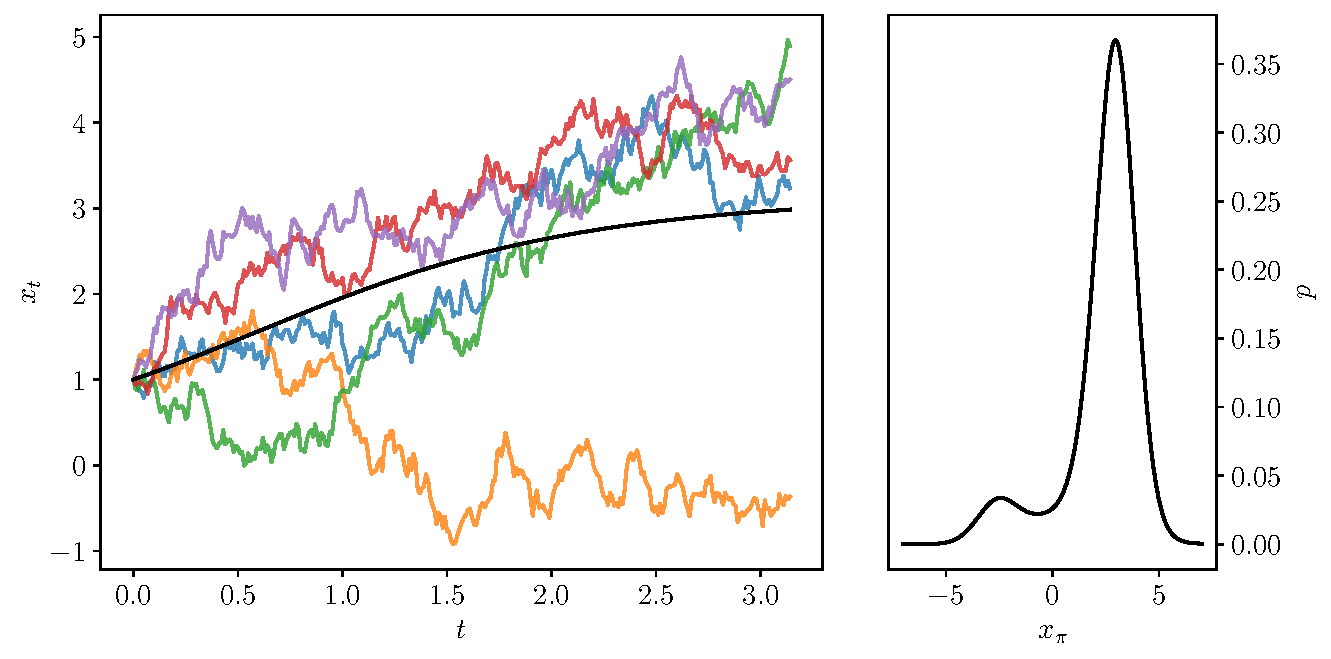
\includegraphics[width=\textwidth]{chp02_background/figures/ou_solution.pdf}
	\caption{(Left) Sample paths of the solution to the stochastic differential equation \(\dif x_t = \sin\!\left(x_t\right)\dif t + \dif W_t\), from the initial condition \(x_0 = 1\) and over the time interval \((0,\pi)\).
		The solution to the corresponding deterministic system \(\od{w_t}{t} = \sin\!\left(w_t\right)\) with the same initial condition is in black.
		(Right) The numerically estimated probability density function of the solution \(x_\pi\), using 10000 samples.}
	\label{fig:sde_sol_sample}
\end{figure}


% Stochastic differential equations also arise as the limit of deterministic slow-fast systems, where the average behaviour of the `fast' dynamics can be shown to converge to the solution of a stochastic differential equation \citep[e.g.]{WongZakai_1965_ConvergenceOrdinaryIntegrals,MelbourneStuart_2011_NoteDiffusionLimits,GottwaldMelbourne_2013_HomogenizationDeterministicMaps}\lb{Maybe some better citations out there.}.
% A review of this theory is provided by \citet{GivonEtAl_2004_ExtractingMacroscopicDynamics}.
% This is particular relevant in climate and physics applications, where \citep{FranzkeEtAl_2015_StochasticClimateTheory}.
% This leads to stochastic parameterisation \citep{BernerEtAl_2017_StochasticParameterizationNew,Palmer_2019_StochasticWeatherClimate}, which we review in more detail in \Cref{sec:stoch_param}.

% The noise driving stochastic differential equations need not be a Wiener process, and can be instead replaced by any semi-martingale, which are a general class of stochastic processes.
% However, we primarily use the Wiener process throughout this thesis due to the aforementioned properties that make it appropriate for modelling scenarios and the ubiquitous use of it across literature and applications.
% We do briefly discuss the possibility of extending some of our work to L\'evy processes, a  more general class of stochastic processes, in \Cref{sec:disc_levy}.



\subsection{Numerical schemes for approximating SDEs}\label{sec:numeric_sdes}
In general, solving a stochastic differential equation analytically is not possible, and so as with ordinary differential equations, we instead look to use numerical schemes to approximate solutions.
However, the solution to a stochastic differential equation is itself a random variable, so a single sample path is not sufficient.
Instead, a numerical SDE scheme involves random sampling (typically of the driving noise process) and produces approximate \emph{realisations} of the solution.
With a large number of these Monte Carlo realisations, one can estimate statistical properties and approximate the distribution of the solution.
The stochastic sampling approach is the gold standard in many applications, most notably climate and weather modelling \citep{Collins_2007_EnsemblesProbabilitiesNew}.

The simplest scheme for numerically solving SDEs is the Euler-Maruyama (EM) method, which is analogous to the Euler method for ODEs \citep{KloedenPlaten_1992_NumericalSolutionStochastic}.
The update step of the EM scheme, with step size \(\delta t\), is
\begin{equation}
	\hat{x}_{t + \delta t} = \hat{x}_{t} + \delta t u\!\left(\hat{x}_t, t\right) + \sqrt{\delta t} \sigma\!\left(\hat{x}_t, t\right) Z_t,
	\label{eqn:em_step}
\end{equation}
where \(Z_t\) is sampled from the standard Gaussian \(\Gauss{0,I}\), and the scheme is initialised as \(\hat{x}_0 = x_0\).
When the initial condition is random, one samples \(\hat{x}_0\) from that distribution.
% The Euler-Maruyama scheme has strong order 0.5, meaning that
% \[
% 	\avg{\norm{x_t - \hat{x}_{t}\left(\Delta t\right)}} = \mathcal{O}\left(\Delta t^{0.5}\right),
% \]
% where \(\hat{x}_t\left(\Delta t\right)\) is the Euler-Maruyama estimate at time \(t\) using step size \(\Delta t\).
There are many other schemes for generating approximate samples of a stochastic differential equation, of varying precision and computational complexity, many of which are given in \citet{KloedenPlaten_1992_NumericalSolutionStochastic}.
Numerical schemes give us access to approximate solutions to otherwise intractable SDEs.
However, this comes at a computational cost: a large number of sample paths is often required to generate convergent statistics and make accurate inferences.
One of the primary aims of this thesis is to overcome this expense by devising alternative ways of approximating and characterising SDE solutions that are computationally cheaper.






% \subsection{The Fokker-Planck equation}\label{sec:fp_eqn}
% The Fokker-Planck (FP) equation is a partial differential equation that describes the time evolution of the probability density function of the solution to a stochastic differential equation.
% The probability density function \(\rho: \R^n \times [0,T] \to [0,\infty)\) for the solution to \cref{eqn:gen_sde} at time \(t \in [0,T]\) is the solution to the corresponding Fokker-Planck equation \citep{Risken_2012_FokkerPlanckEquationMethods}
% \begin{equation}
% 	\dpd{\rho}{t} = \frac12\nabla\cdot\nabla\cdot\left(\rho\sigma\sigma^{\T}\right) - \nabla\cdot\left(\rho u\right)
% 	\label{eqn:fp_eqn}
% \end{equation}
% subject to some initial density \(\rho\left(x,0\right)\) given by the initial condition to \cref{eqn:gen_sde}.
% For a fixed and deterministic initial condition \(y_0 = x\), the corresponding initial condition to \cref{eqn:fp_eqn} is the Dirac-delta distribution centred at \(x\).
% To ensure that the solution is a valid probability density function on \(\R^n\), for any \(t \in [0,T]\), \(\rho\) must satisfy
% \begin{subequations}\label{eqn:fp_valid_pdf}
% 	\begin{align}
% 		\int_{\R^n}{\rho\left(x, t\right)\dif x} = 1, \label{eqn:fp_valid_pdf_norm} \\
% 		\lim_{x \to \infty}\rho\left(x,t\right) = 0. \label{eqn:fp_valid_pdf_limit}
% 	\end{align}
% \end{subequations}
% Solving the Fokker-Planck equation provides an alternative method for finding the solution to a stochastic differential equation; rather than dealing with stochastic quantities, we instead seek solutions to the
% However, the Fokker-Planck equation cannot be solved analytically except for simple cases and there are several practical difficulties in attempting to solve it numerically.
% These difficulties include:
% \begin{itemize}
% 	\item \textbf{Dimensionality:} In high-dimensional systems, solving the Fokker-Planck equation numerically is computationally prohibitative, requiring a small spatial discretisation to be accurate.
% 	\item \textbf{Boundary conditions:} The Fokker-Planck equation is often defined on an unbounded domain with the zero-limit constraint \cref{eqn:fp_valid_pdf_limit}, which presents computational difficulties.
% 	\item \textbf{Normality constraints:} The Fokker-Planck equation must be solved with the additional normality condition \cref{eqn:fp_valid_pdf_norm}, which enforces an additional constraint on any numerical solution.
% \end{itemize}
% It is generally accepted that these difficulties mean that the computational cost of solving the Fokker-Planck equation is too high in \(3\)- or higher dimensions \citep{ZhaiEtAl_2022_DeepLearningMethod,Li_2019_DatadrivenMethodSteady,AllawalaMarston_2016_StatisticsStochasticallyForced}.

% \td{Perhaps comment on how the FP equation arises in other settings, and is a generalisation of the advection-diffusion equation and similar. Hence learning stuff about the solution to the SDE also tells us about the FP equation.}

% \subsubsection{Relationship to the classical advection-diffusion equation}
% The advection-diffusion equation describes the time-evolution of a passive and inert scalar quantity, such as temperature, salinity

% \citep{Visser_2008_LagrangianModellingPlankton}

% Let \(c \colon \Omega_0 \times [0,T] \to [0, \infty)\) denote the concentration of a passive and inert scalar quantity, then the classical advection-diffusion equation is
% \begin{equation}\label{eqn:advec_diff}
% 	\dpd{c}{t} = - \nabla\cdot \left(v\!\left(x,t\right)c\!\left(x,t\right)\right) + \nabla\cdot\left(K\!\left(x,t\right)\nabla c\!\left(x,t\right)\right), \quad c\!\left(x,0\right) = c_0\!\left(x\right),
% \end{equation}
% where \(v\) denotes the flow velocity dictating the advection (displacement) of the tracer, and \(K\) is a matrix describing the diffusion (dispersion) of \(c\).




% If we set \(u\!\left(x,t\right) = v\!\left(x,t\right) + \nabla \cdot K\!\left(x,t\right)\) and \(\sigma\!\left(x,t\right)\sigma\!\left(x,t\right) = K\!\left(x,t\right)\), then the Fokker-Planck equation \cref{eqn:fp_eqn} is equivalent to the advection-diffusion equation \cref{eqn:advec_diff}.
% Thus, the evolution of the tracer concentration under \cref{eqn:advec_diff} can be equivalently considered as the probability density function of solutions to the stochastic differential equation
% \begin{equation}\label{eqn:ad_sde}
% 	\dif x_t = \left[u\!\left(x_t, t\right) + \nabla \cdot K\!\left(x_t, t\right)\right]\dif t + \kappa\!\left(x_t, t\right)\dif W_t, \quad x_t \sim \hat{c}_0,
% \end{equation}
% where \(\kappa\) is any matrix-valued function satisfying \(K \equiv \kappa\kappa^{\T}\), and
% \[
% 	\hat{c}_0\!\left(x\right) = \frac{c_0\!\left(x\right)}{\int_{\Omega_0}c_0\!\left(z\right)\dif z},
% \]
% is the initial density of \cref{eqn:advec_diff} normalised to describe a probability density function.
% Assuming that the total concentration tracer is conserved, that is
% \[
% 	\int_{\Omega_t}{c\!\left(z,t\right)\dif z} = \int_{\Omega_0}{c_0\!\left(z\right)\dif t}
% \]
% for all \(t \in [0,T]\), then we can recover \(c\) from the probability density function \(\rho\) corresponding to \cref{eqn:ad_sde} as
% \[
% 	c\!\left(x,t\right) = \rho\!\left(x,t\right)\int_{\Omega_0}{c_0\!\left(z\right)\dif t}.
% \]
% An implication of this connection is that the theory and computations for stochastic differential equations developed throughout this thesis can be applied to \emph{any} scalar field that is modelled with an advection-diffusion type equation.


% \subsubsection{Green's function method}
% The Fokker-Planck equation is linear, so we can apply a technique known as Green's function method (for an example of this approach on a linear SDE, see Section 3.2 of \citet{Risken_2012_FokkerPlanckEquationMethods}) in order to understand the behaviour of solutions with non-fixed initial conditions.
% Let \(\mathcal{P}_t\set{\rho_0}\) denote the solution operator of \cref{eqn:fp_eqn} with initial density \(\rho_0\colon \R^n \to \R^n\).
% Then, since \cref{eqn:fp_eqn} is a linear equation, \(\mathcal{P}_t\) is a linear operator.
% Now, let \(x_0 \in \R^n\) be an arbitrary fixed point, and consider the fundamental solution, or Green's function,
% \[
% 	G_t\left(x; x_0\right) \coloneqq \mathcal{P}_t\set{\delta_{x_0}}\!\left(x\right).
% \]
% That is, \(G_t\left(x; x_0\right)\) is the solution to the Fokker-Planck equation with the Dirac-delta initial condition \(\delta_{x_0}(x) = \delta\left(x - x_0\right)\), which is equivalent to the SDE \cref{eqn:gen_sde} with the deterministic and fixed initial condition \(y_0 = x_0\).
% The Green's function \(G_t\) is equivalently the transition probability function of the SDE solution \(x_t\) as a stochastic process.
% Now, using the sampling property of the Dirac-delta function, for a general initial density \(\rho_0\colon \R^n \to \R^n\),
% \[
% 	\rho_0(x_0) = \int_{\R^n}{\rho_0\left(x\right)\delta_{x_0}\left(x\right)\dif x}.
% \]
% Since \(\mathcal{P}_t\) is linear,
% \begin{equation}
% 	\mathcal{P}_t\set{\rho_0}\!\left(x_0\right) = \int_{\R^n}{\rho_0\!\left(x\right)\mathcal{P}_t\set{\delta_{x_0}}\!\left(x\right)\dif x} = \int_{\R^n}{\rho_0\!\left(x\right) G_t\!\left(x; x_0\right)\dif x}.
% 	\label{eqn:fp_greens_trick}
% \end{equation}
% An implication of \cref{eqn:fp_greens_trick} is that for a given stochastic differential equation, we only need to understand the behaviour of solutions subject to a fixed (albeit arbitrary) initial condition.


\section{Lagrangian coherent structures}\label{sec:bkg_lcs}

\begin{figure}
	\begin{center}
		\begin{subfigure}[t]{0.49\textwidth}
			\includegraphics[width=\textwidth]{chp02_background/figures/dwh_cropped}
			\caption{An oil slick from the \emph{Deepwater Horizon} oil spill in 2010 (NASA Image of the Day, May 19, 2010).
				The southwards extension of the slick appeared unexpectedly.}
			\label{fig:lcs_deepwater}
		\end{subfigure}
		\begin{subfigure}[t]{0.49\textwidth}
			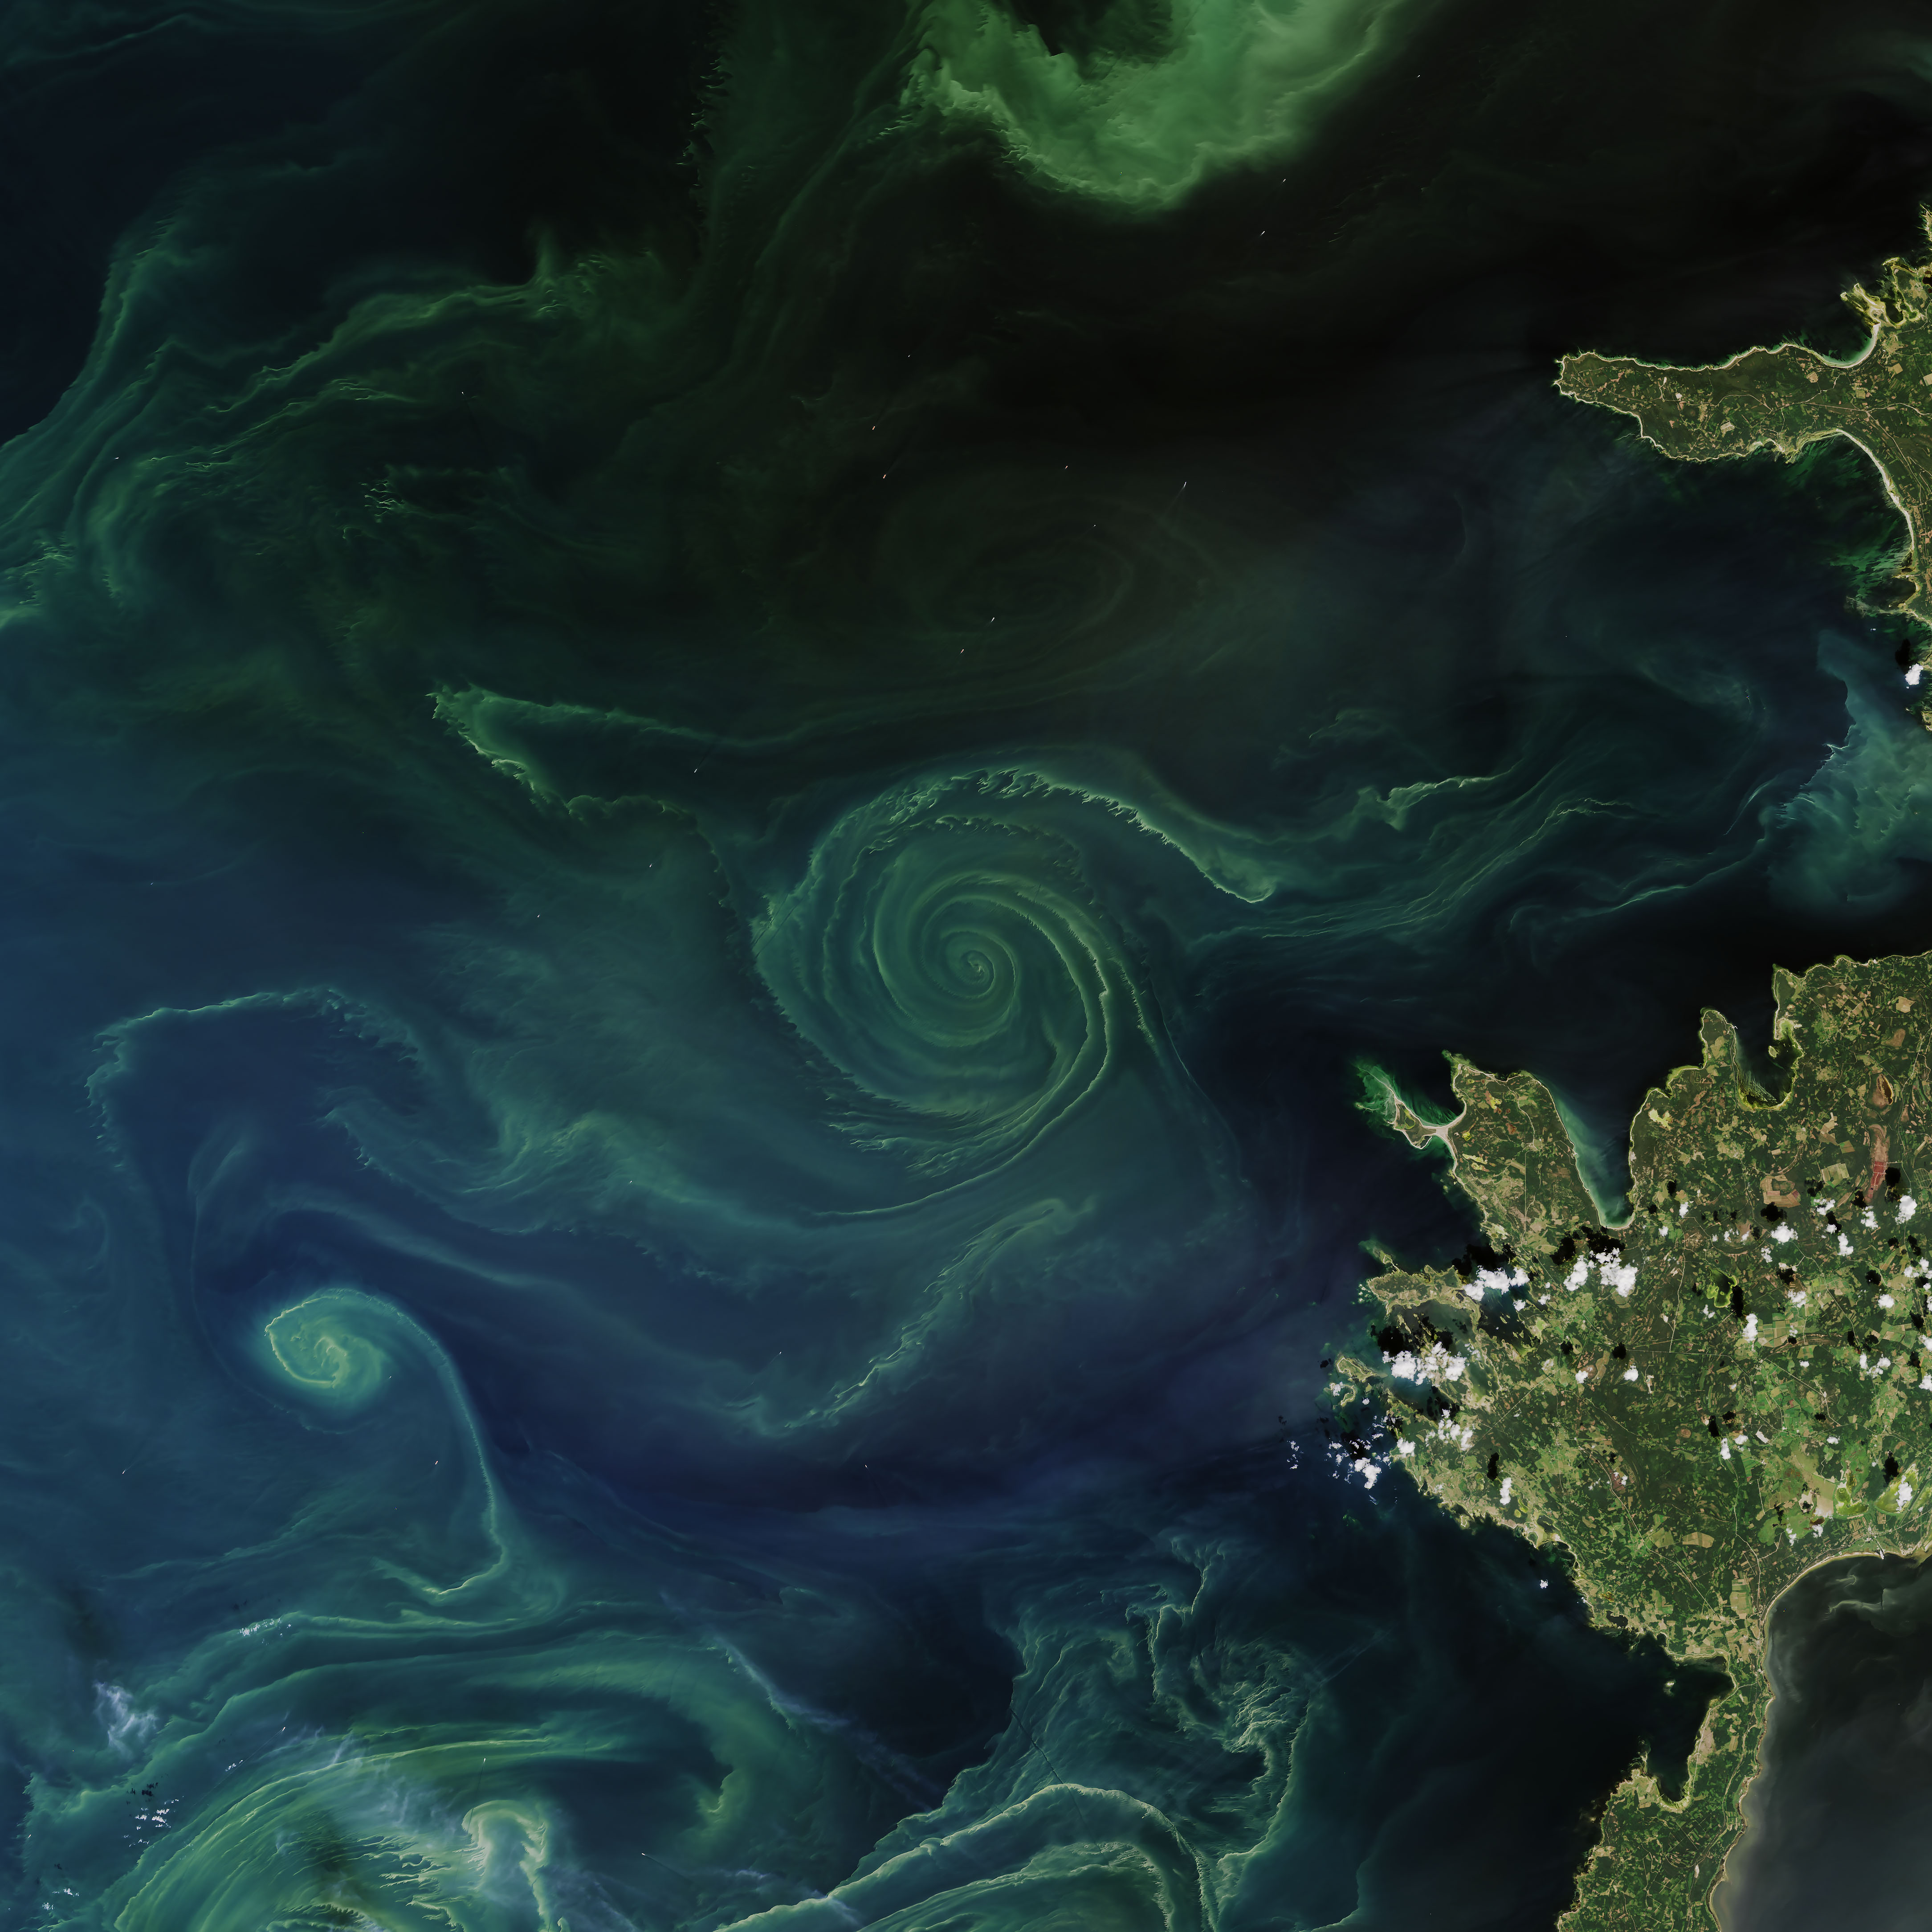
\includegraphics[width=\textwidth]{chp02_background/figures/photoplankton}
			\caption{Phytoplankton blooms in the Baltic Sea (NASA Earth Observatory, July 18, 2018).
				The structure of these blooms reflect the underlying flow of the Sea.}
			\label{fig:lcs_phyto}
		\end{subfigure}
		\begin{subfigure}[t]{\textwidth}
			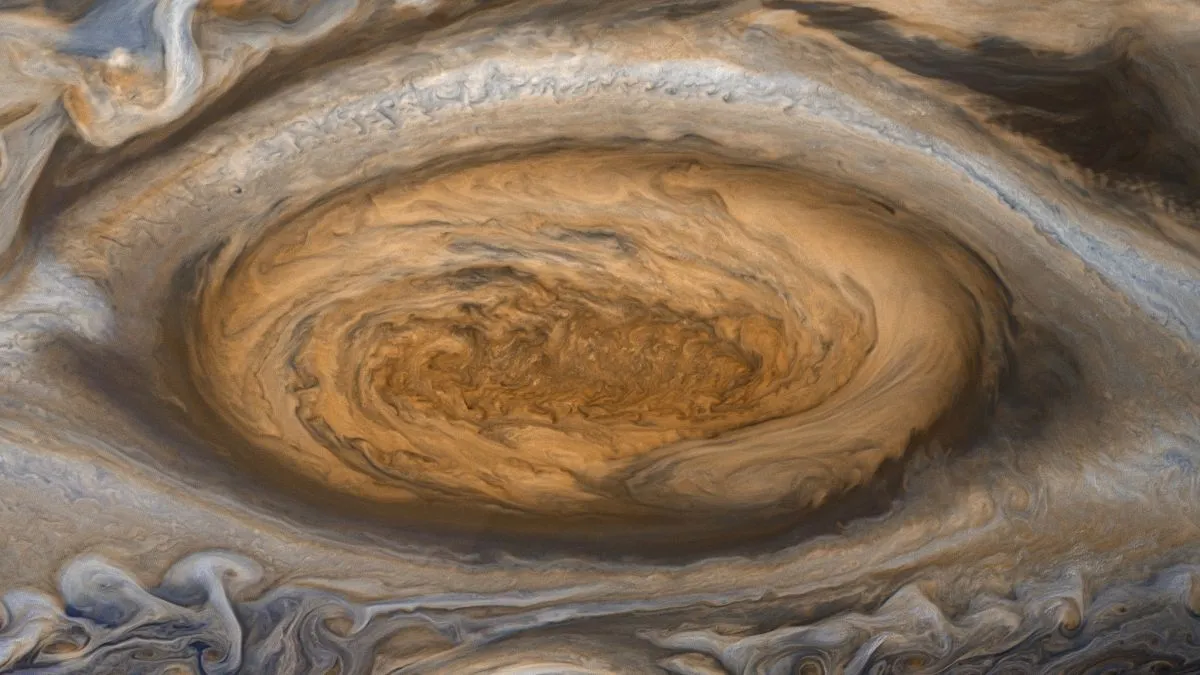
\includegraphics[width=\textwidth]{chp02_background/figures/red_spot.png}
			\caption{Jupiter's Great Red Spot, as photographed by the Voyager 1 probe (NASA/JPL-Caltech and processed by Bj\"{o}rn J\'{o}nsson, March 5, 1979).
			The storm is an example of a vortex or eddy within the atmospheric flow of the planet.}
		\end{subfigure}
		% \begin{subfigure}[t]{0.49\textwidth}
		% 	% 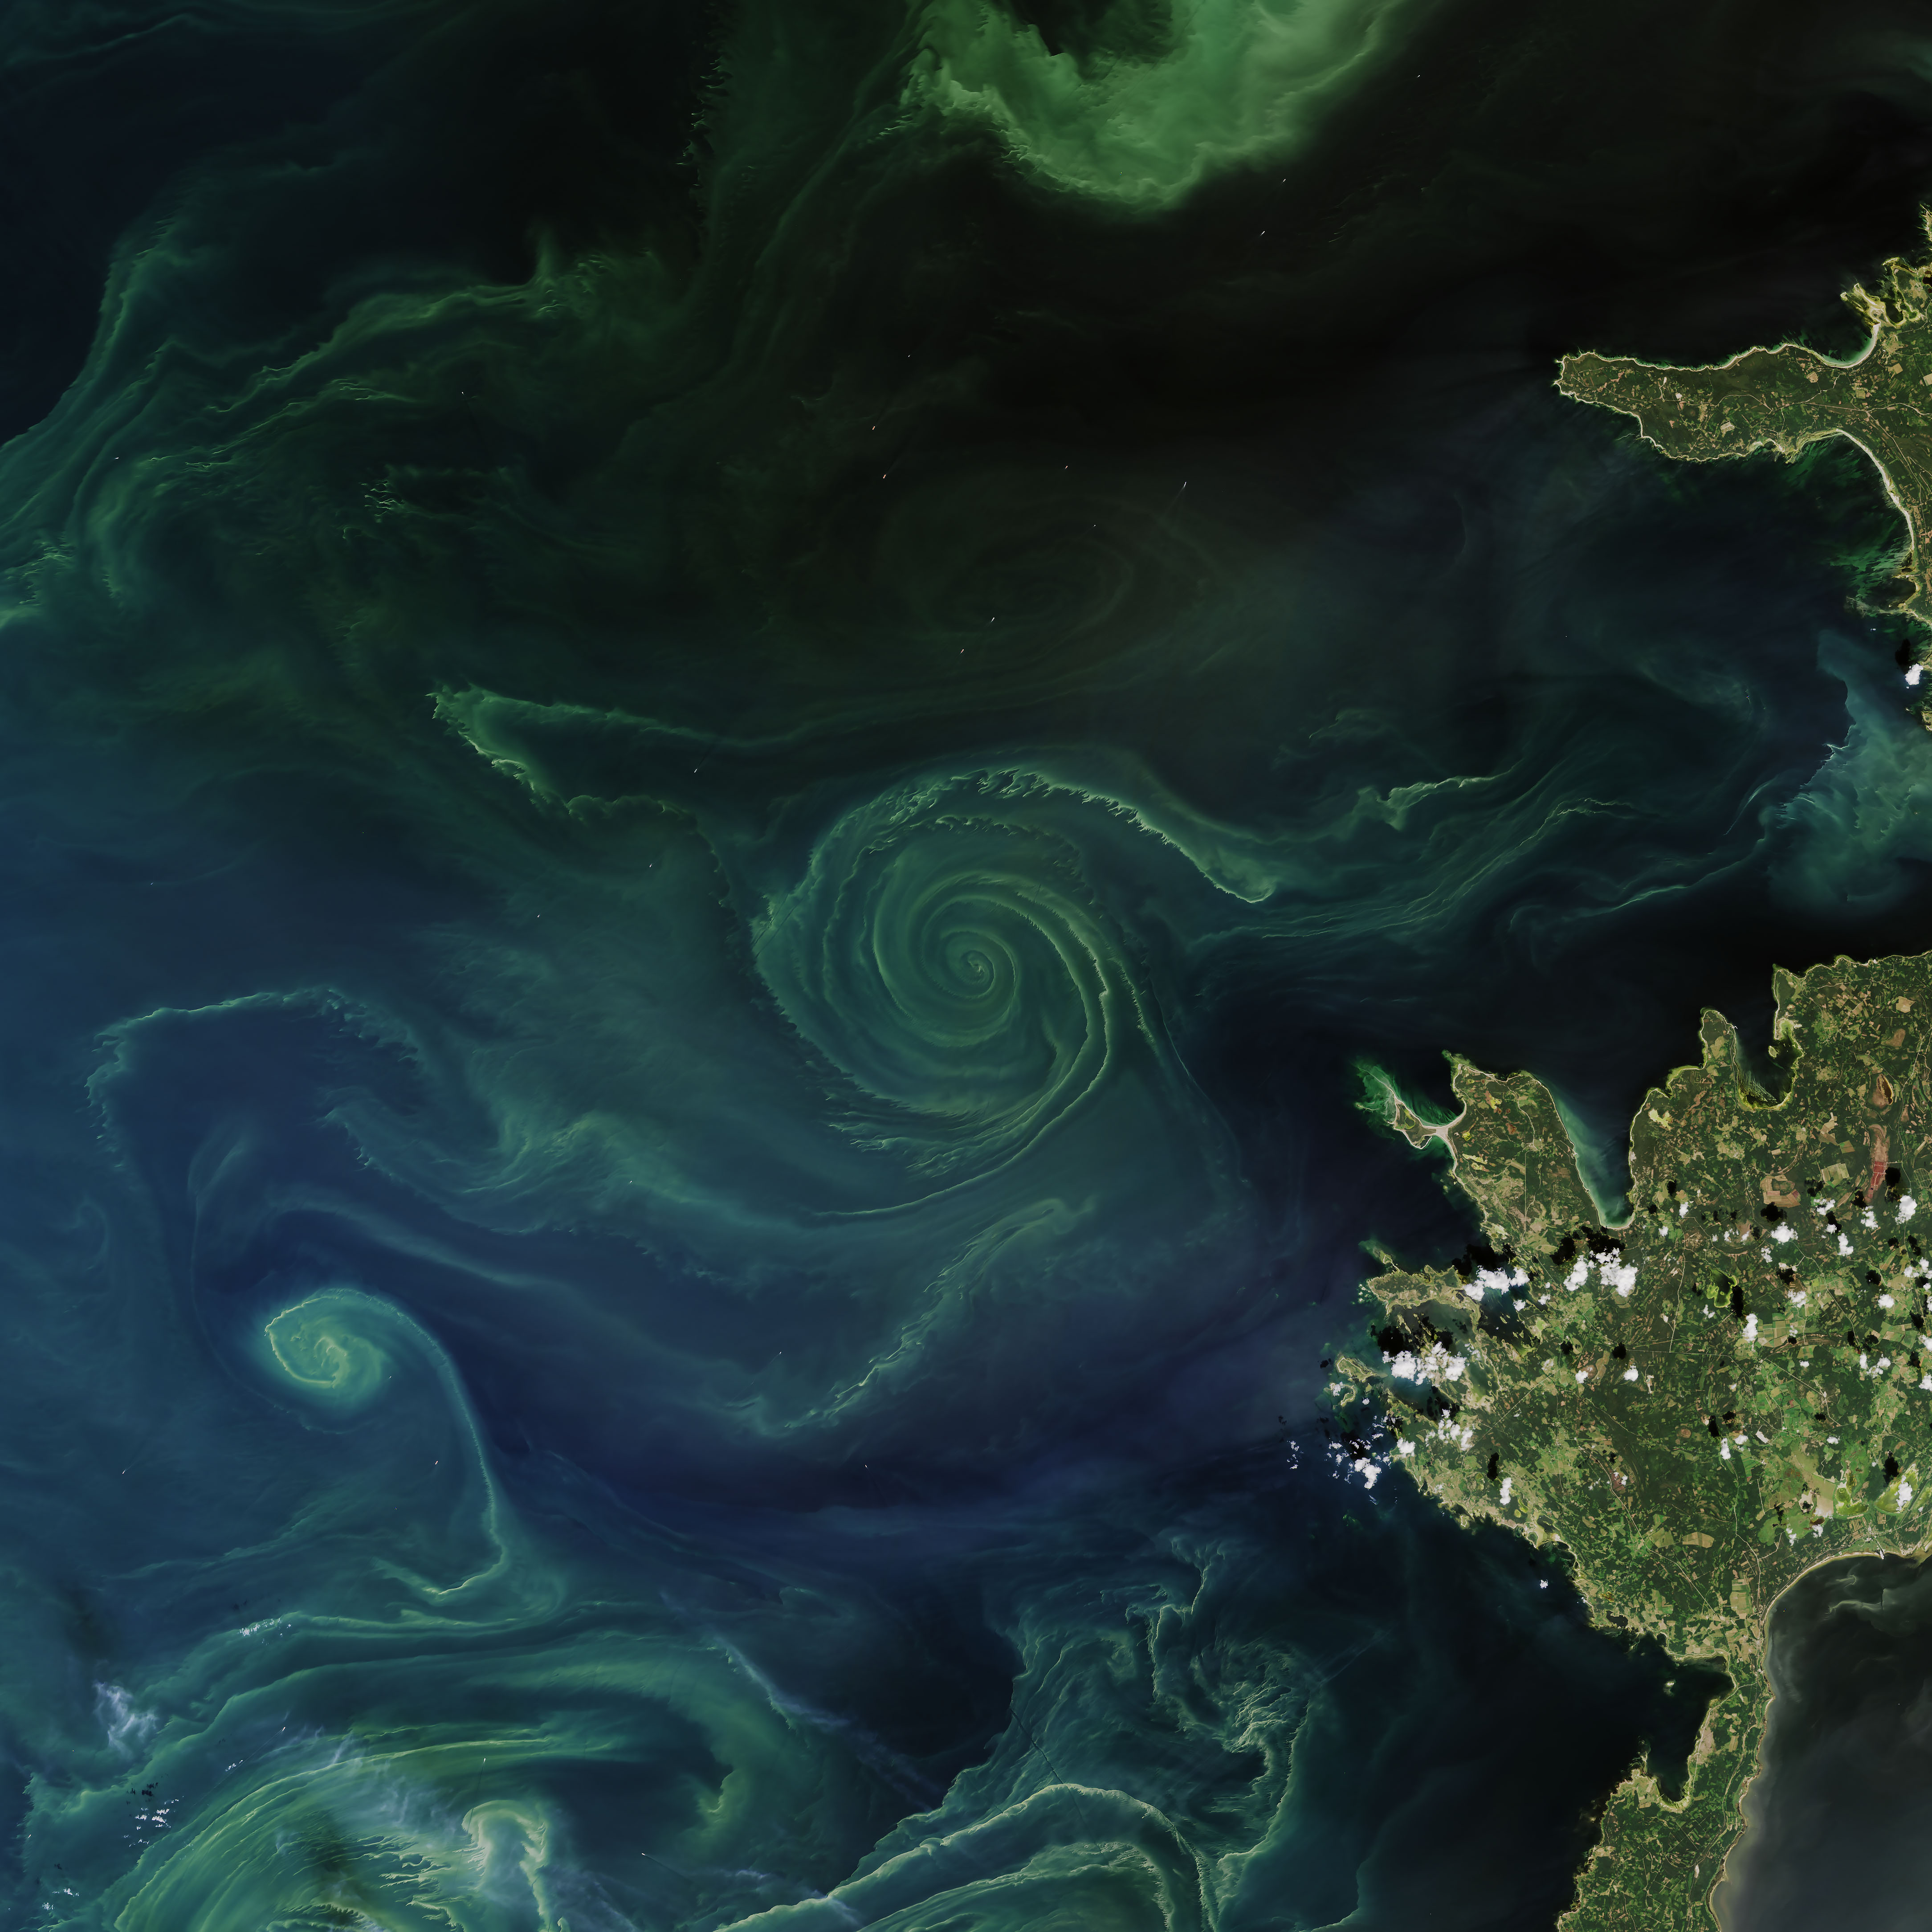
\includegraphics[width=\textwidth]{chp02_background/figures/photoplankton}
		% 	\td{Get one more example!}
		% 	\caption{}
		% \end{subfigure}
		\caption{Examples of coherent patterns emerging in fluid flows observed in nature.}
		\label{fig:lcs_examples}
	\end{center}
\end{figure}

In this section, we take a brief sojourn into the field of Lagrangian coherent structures (LCSs), which provide qualitative insight into the behaviour of a dynamical system, particularly in the context of fluid flows.
Although LCSs are not the primary focus of this work, the field provides potential applications for our uncertainty quantification, that builds upon preliminary work by \citet{Balasuriya_2020_StochasticSensitivityComputable,Balasuriya_2020_UncertaintyFinitetimeLyapunov} and \citet{BadzaEtAl_2023_HowSensitiveAre}.
There is no universally accepted definition of a coherent structure, but typically these are structures within a flow that remain together over the time-evolution of the system and separate the spatial domain into regions with qualitatively different behaviour \citep{BalasuriyaEtAl_2018_GeneralizedLagrangianCoherent}.
\Cref{fig:lcs_examples} shows examples of coherent structures in observed fluid flows, which can be considered LCSs.
These are structures such as vortices, eddies, and jets that influence the transport of material within the fluid.
For instance, in \Cref{fig:lcs_deepwater,fig:lcs_phyto}, the observed patterns of the oil slick and phytoplankton blooms respectively reflect the behaviour of the underlying ocean flow and are influenced by jet- and eddy-like structures.

In a steady system (that is, the vector field \(u\) in \cref{eqn:det_ode} is independent of time), we can gain this insight by using classical methods in dynamical systems, such as phase portrait analysis and identifying unstable and stable manifolds.
For example, solution trajectories cannot intersect unstable and stable manifolds, and so these manifolds can act as barriers for the transport of material within a flow.
However, when the system is non-autonomous (that is, the vector field explicitly depends on time \(t\)), these structures can themselves vary with time and the problem of identifying them is far more non-trivial.
Another complication is that in practice, the data driving a system is only available over a finite timeframe, whereas classical dynamical systems techniques often tell us about the long-term (in the infinite time limit) behaviour of solutions.
Lagrangian coherent structure theory provides a mathematical framework for defining and identifying such structures within a flow \citep{BalasuriyaEtAl_2018_GeneralizedLagrangianCoherent}.
There are many procedures and heuristics for extracting these regions from a given flow, which draw upon different mathematical techniques, including classical dynamical system theory, variational calculus, transfer operators, and statistical clustering.
Detailed reviews of approaches to Lagrangian coherent structure extraction are provided by \citet{PeacockDabiri_2010_IntroductionFocusIssue}, \citet{HadjighasemEtAl_2017_CriticalComparisonLagrangian}, and \citet{BalasuriyaEtAl_2018_GeneralizedLagrangianCoherent}.

Coherent structures can provide valuable qualitative insight into the behaviour of a flow, by providing an outline of the transport properties and underlying dynamics.
An example is in the study of the spread of the oil slick resulting from the 2010 Deepwater Horizon disaster in the Gulf of Mexico (see \Cref{fig:lcs_deepwater}).
Investigations showed that the behaviour of the slick, including a sudden and unexpected extension of the slick, could be understood and therefore predicted in future cases by using Lagrangian coherent structures and the insight they provide \citep{OlascoagaEtAl_2013_DrifterMotionGulf,OlascoagaHaller_2012_ForecastingSuddenChanges,MezicEtAl_2010_NewMixingDiagnostic}.
This approach explained dynamics that were otherwise poorly understood because of the time-varying and complex nature of the flow.

One of the most well-studied and frequently used procedures for extracting Lagrangian coherent structures is via the finite-time Lyapunov exponent (FTLE), which is a measure quantifying the stretching of infinitesimal regions of the flow over a time period.
The FTLE can be computed as a scalar field over a set of initial conditions, from which the maximising ridges can correspond to flow barriers \citep{ShaddenEtAl_2005_DefinitionPropertiesLagrangian}.
Importantly, the finite-time Lyapunov exponent can be computed only using the gradients of the flow map, which ensures a highly practical and flexible procedure that can be used across many different contexts.
The FTLE is an example of a common class of LCS methods that first compute a field over a set of initial conditions and then extract coherent structures based on that field.

% One of the best known procedures for extracting LCSs is via the finite-time Lyapunov exponent (FTLE) \citep{ShaddenEtAl_2005_DefinitionPropertiesLagrangian}, which is a measure quantifying the stretching of infinitesimal regions of a flow over a finite time period.
% Take an initial condition \(x\) and let \(F_0^t\) represent the flow map of our system over the time interval \([0,t]\).
% We wish to quantify the impact of a small change in the initial condition on the flow at time \(t\), so take \(\delta\) as a small and arbitrary perturbation to \(x\).
% Then, we measure the \emph{stretching} in the direction of \(\delta\) with
% \[
% 	s\!\left(x, \delta\right) = \frac{\norm{F_0^t\!\left(x + \delta\right) - F_0^t\!\left(x\right)}}{\norm{\delta}}
% \]
% For sufficiently small \(\delta\), we can replace the mapped perturbation with a linearisation of the flow map about \(x\), that is
% \[
% 	s\!\left(x, \delta\right) \approx \frac{\norm{\nabla F_0^t\!\left(x\right) \delta}}{\norm{\delta}}.
% \]
% % \Cref{fig:ftle_illustr} provides a pictorial representation of this calculation; a small !!!!!
% Taking the supremum over all possible perturbations \(\delta\), we have
% \[
% 	\sup_{\delta \in \R^n, \, \delta \neq 0}s\!\left(x, \delta\right) \approx \norm{\nabla F_0^t\!\left(x\right)},
% \]
% which quantifies the stretching about the trajectory \(F_0^t\!\left(x\right)\).
% The finite-time Lyapunov exponent is then computed as
% \begin{equation}
% 	\mathrm{FTLE}_0^t\!\left(x\right) = \frac{1}{\abs{t}}\ln\!\left(\norm{\nabla F_0^t\!\left(x\right)}\right).
% 	\label{eqn:ftle_defn}
% \end{equation}
% Note that the operator norm \(\norm{\nabla F_0^t\!\left(x\right)}\) in \cref{eqn:ftle_defn} can be readily computed as the square root of the largest eigenvalue of the Cauchy-Green tensor \(\left[\nabla F_0^t\!\left(x\right)\right]^{\T}\nabla F_0^t\!\left(x\right)\).
% Over the set of initial conditions, the FTLE is a scalar field that measures for each initial condition the stretching and contraction along the resulting trajectory.
% The FTLE is a measure of exponential stretching (hence the scalings in \cref{eqn:ftle_defn}), and provides insight into the nonlinearity of a system, including as an indicator of one defining feature of chaos.
% It was shown by \citet{ShaddenEtAl_2005_DefinitionPropertiesLagrangian} that the maximising ridges of the FTLE field can correspond to flow barriers, and so by finding these ridges, one can extract coherent structures for the flow.


% In \Cref{fig:gs_lcs}, we compute the FTLE field of our Gulf Stream velocity model over a timespan of 7 days.



% \begin{figure}
% 	\begin{center}
% 		\begin{subfigure}{0.49\textwidth}
% 			\includegraphics[width=\textwidth]{chp02_background/figures/gulf_stream_motivation/ftle.pdf}
% 			\caption{The finite-time Lyapunov exponent field.}
% 		\end{subfigure}
% 		\begin{subfigure}{0.49\textwidth}
% 			\caption{Maximising ridges of the FTLE field.}
% 		\end{subfigure}
% 		\caption{The finite-time Lyapunov exponent field computed, and corresponding maximising ridges.
% 			This is an example of using a scalar field to extract Lagrangian coherent structures from a fluid flow.
% 			The resulting maximises ridges indicate a skeleton of the Gulf Stream.}
% 		\label{fig:gs_lcs}
% 	\end{center}
% \end{figure}


Most well-established LCS frameworks and extraction procedures are purely deterministic, in that they are defined and computed solely in terms of the behaviour of the underlying ordinary differential equation.
However, uncertainty in such systems is inevitable in practice and these methods fail to account explicitly for this.
Accordingly, there is an emerging interest \citep{Balasuriya_2020_StochasticApproachesLagrangian} in extending LCS theory to stochastic settings.
There are two primary ways in which stochastic has been recently investigated in the LCS community:
\begin{romanate}
	\item in creating novel procedures that explicitly account for such ongoing uncertainty, such as by using properties of corresponding stochastic systems.
	For example, see (in \Cref{sec:s2_summ}) stochastic sensitivity introduced by \citet{Balasuriya_2020_StochasticSensitivityComputable}, model sensitivity introduced by \citet{KaszasHaller_2020_UniversalUpperEstimate}, and the finite-time divergence rate by \citet{BranickiUda_2023_PathBasedDivergenceRates}.
	These are scalar fields defined on initial conditions that measure the certainty in the corresponding deterministic trajectories and can distinguish coherent regions in similar ways to deterministic methods.
	As another example, \citet{DennerEtAl_2016_ComputingCoherentSets} directly compute coherent sets by working with a discretised Fokker-Planck equation, which is a partial differential equation that governs the probability density function of an SDE solution (an overview is provided in \Cref{sec:disc_fp}).
	This Fokker-Planck approach extends the transfer operator method of \citet{Froyland_2013_AnalyticFrameworkIdentifying}, which is a popular method for LCS detection and extraction by encoding how densities are pushed forward by the flow.
	Until recently, the transfer operator, at least in the context of Lagrangian analysis, has been viewed as purely deterministic but provides a framework for naturally including velocity field uncertainties \citep{Balasuriya_2020_StochasticApproachesLagrangian}.

	\item in understanding the direct impact of velocity uncertainty on well-established deterministic LCS measures.
	\citet{BadzaEtAl_2023_HowSensitiveAre} provide a systematic analysis, using Monte Carlo simulation and summary statistics to evaluate the robustness of several common LCS extraction schemes to velocity uncertainty.
	% It is shown that LCS methods that directly account for this uncertainty, such as stochastic sensitivity \citep{Balasuriya_2020_StochasticSensitivityComputable}, are the most robust.
	The finite-time Lyapunov exponent has received particular attention, with recent studies aiming to quantify the impact of velocity field uncertainty on the FTLE computation: \citet{GuoEtAl_2016_FiniteTimeLyapunovExponents} use stochastic simulation and statistical analysis, \citet{Balasuriya_2020_UncertaintyFinitetimeLyapunov} provides theoretical error bounds on the FTLE computation, and \citet{YouLeung_2021_ComputingFiniteTime} propose an approach for computing the (statistically) expected FTLE field.

\end{romanate}
In this thesis, we are primarily interested in point (i), by exploring how our characterisations of uncertainty can be applied to extract coherent structures.
This is directly extending the stochastic sensitivity of \citet{Balasuriya_2020_StochasticSensitivityComputable}, which is summarised in \Cref{sec:s2_summ}.
We will also discuss (in \Cref{sec:s2_disc}) how we anticipate our work could be applied to point (ii), as a quantification of uncertainty in computations involving the flow map in other LCS schemes.




\section{Stochastic sensitivity}\label{sec:s2_summ}
To conclude our background and motivation, this section summarises stochastic sensitivity, a measure of uncertainty in differential equations introduced by \citet{Balasuriya_2020_StochasticSensitivityComputable}.
These tools are \emph{computable} given only velocity data, which enables an efficient quantification of uncertainty in a stochastic system with no need for bulk simulation.
Stochastic sensitivity (also termed \(S^2\) in both notation and prose) was originally provided for 2-dimensional systems only, and the primary motivation was to understand the impact of velocity field uncertainty on fluid flows.
Given possibly time-dependent velocity data \(u\colon \R^2 \times [0,T] \to \R^2\), \citet{Balasuriya_2020_StochasticSensitivityComputable} considers the evolution of solutions to the ordinary differential equation
\begin{equation}\label{eqn:s2_ode}
	\dod{x_t}{t} = u\!\left(x_t, t\right),
\end{equation}
subject to some fixed initial condition \(x_0\).
The velocity field \(u\) is \emph{Eulerian}, in that it describes the fluid velocity at a given point in space and time.
The trajectories that solve \cref{eqn:s2_ode} are \emph{Lagrangian} and correspond to the movement of idealised infinitesimal particles within the flow.
These Lagrangian trajectories are summarised by the flow map \(F_s^t\) of \cref{eqn:s2_ode}.
As we have continued to emphasise, the velocity field \(u\) is in practice subject to unavoidable uncertainties.
\citet{Balasuriya_2020_StochasticSensitivityComputable} aims to quantify the impact of this Eulerian uncertainty, directly attributed to \(u\), on the Lagrangian trajectories arising from integrating the velocity field.
% In most practical situations, the Eulerian velocity data driving ocean and atmospheric models relies upon measurements of estimates obtained on a low resolution spatial discretisation.
% \citet{Balasuriya_2020_StochasticSensitivityComputable} introduces stochastic sensitivity as a new tool for directly quantifying the impact of Eulerian uncertainty on Lagrangian trajectories.

To directly account for these unresolved sources of uncertainty, the `true' Lagrangian trajectories evolve as solutions to the stochastic differential equation
\begin{equation}
	\sde{y_t}{u\!\left(y_t, t\right)}{\epsilon\sigma\!\left(y_t, t\right)}, \quad y_0 = x_0
	\label{eqn:s2_sde},
\end{equation}
where \(0 < \epsilon \ll 1\) is a parameter quantifying the scale of the noise, \(\sigma\colon	\R^2\times[0,T] \to \R^{2\times 2}\) is the \(2\times 2\) diffusion matrix, and \(W_t\) is the canonical 2-dimensional Wiener process.
In the original formulation \citep{Balasuriya_2020_StochasticSensitivityComputable}, \(\epsilon\) is a dimensionless parameter and \(\sigma\) is dimensional, but an alternative scaling technique relates \(\epsilon\) to spatial and velocity uncertainty scales in the data (see the follow-up work by \citet{Balasuriya_2020_UncertaintyFinitetimeLyapunov}, \citet{FangEtAl_2020_DisentanglingResolutionPrecision}, and \citet{BadzaEtAl_2023_HowSensitiveAre} for example).
Since \(\sigma\) can vary by both space and time, the noise is permitted to be multiplicative.
The diffusion matrix \(\sigma\) is specified \emph{a priori}, based on any knowledge of how uncertainty varies with space and time, e.g.\ from experimental considerations, observation error estimates, physics-informed models, etc.
If no such prior information is known, then \(\sigma \equiv I\), the \(2 \times 2\) identity matrix, is the default choice.

Next, to quantify uncertainty at a time \(t\), \citet{Balasuriya_2020_StochasticSensitivityComputable} defined the random variable \(z_\epsilon\left(x_0\right)\) as
\[
	z_\epsilon\!\left(x_0\right) \coloneqq \frac{y_t - F_0^t\!\left(x_0\right)}{\epsilon},
\]
which captures the random deviation between the ``true'' stochastic trajectories and the deterministic flow map.
The aim was to compute certain statistics of \(z_\epsilon\).
To derive such quantities that can be computed in practice, \citet{Balasuriya_2020_StochasticSensitivityComputable} considers the signed projection of \(z_\epsilon\!\left(x_0\right)\) onto a ray emanating from the deterministic position \(F_0^t\!\left(x_0\right)\) in the direction \(\theta\), defining
\[
	P_\epsilon\!\left(x_0,\theta\right) \coloneqq \hat{n}^{\T}\!\left(\theta\right) z_\epsilon\!(x_0), \quad \hat{n}\!\left(\theta\right) = \begin{bmatrix}
		\cos{\theta} \\
		\sin{\theta}
	\end{bmatrix}.
\]
where \(\theta \in \left[-\pi/2, \pi/2\right)\).
The statistics of \(z_\epsilon\!\left(x_0\right)\) and \(P_\epsilon\!\left(x_0,\theta\right)\) are considered in the limit as \(\epsilon\downarrow 0\), which provides a characterisation of the uncertainty of the model that is \emph{independent} of the scale of the noise.
\citet{Balasuriya_2020_StochasticSensitivityComputable} defines two measures of uncertainty from the variance of \(P_\epsilon\) in this limit:  %provided computable expressions for the mean and variance of \(P_\epsilon\left(x,\theta\right)\) in this limit of small noise, which we summarise here.
% For proofs of these results, see the appendices of \citet{Balasuriya_2020_StochasticSensitivityComputable}.

\begin{definition}[\citealt{Balasuriya_2020_StochasticSensitivityComputable}]
	\begin{alpharate}
		\item The \textbf{anisotropic uncertainty} is a scalar field \(A: \R^2\times\left[-\pi/2, \pi/2\right) \to [0,\infty)\) defined by
		\[
			A\!\left(x_0,\theta\right) \coloneqq \sqrt{\lim_{\epsilon\downarrow 0}\var{P_\epsilon\!\left(x_0,\theta\right)}}.
		\]

		\item The \textbf{stochastic sensitivity} is a scalar field \(S: \R^2 \to [0,\infty)\) defined by
		\[
			S^2\!\left(x_0\right) \coloneqq \lim_{\epsilon\downarrow 0}\sup_{\theta}{\var{P_\epsilon\!\left(x_0,\theta\right)}}.
		\]
	\end{alpharate}
\end{definition}

\begin{figure}
	\centering
	\begin{tikzpicture}[scale=2]
		\pgfmathsetseed{1}

		% Actual path
		\draw (1,1) .. controls (2.5,-0.5) and (4,1.4) .. (5, 0.5);

		% Stochastic path -- just place a random walk between specified points
		\draw[color=ForestGreen, decorate, decoration={random steps, segment length = 1pt, amplitude=2pt}] (1,1) .. controls (2.5, -0.2) and (3.7,2.7) .. (6.4, 2.1);

		% S2 quantities
		\path[-{Latex[length=3mm, width=1.5mm]},blue] (5,0.5) edge node[left, xshift=-5pt] {\(\epsilon z_\epsilon\!\left(x_0\right)\)} (6.4, 2.1);
		% Calculation here: fix theta, the angle of the projection. Length of the vector between det point and end of projection is l*sin(n), where l is the length of the vector between the det and stoch points, and n = pi/2 - phi + theta, where phi is the angle of the vector between the det and stoch points.
		\def\vecl{sqrt(1.4^2 + 1.6^2)};
		\def\projtheta{pi/7};
		\def\projphi{atan(1.6 / 1.4) * pi / 180}
		\path[red] (5,0.5) edge node[right, xshift=5pt] {\(\epsilon P_{\epsilon}\!\left(x_0,\theta\right)\)} ({5 +\vecl*cos((\projphi - \projtheta) r) * cos(\projtheta r)}, {0.5 + \vecl* cos((\projphi - \projtheta) r) * sin(\projtheta r)});

		\path[dashed, gray] (6.4, 2.1) edge ({5 + \vecl * cos((\projphi - \projtheta) r) * cos(\projtheta r)}, {0.5 + \vecl * cos((\projphi - \projtheta) r) * sin(\projtheta r)});

		% Reference angle
		\path[dashed,gray] (5,0.5) edge (7,0.5);
		\draw[gray] (5.5,0.5) arc (0:{\projtheta * 180 / pi}:0.5) node[midway, xshift=5pt, yshift=2pt] {\(\theta\)};

		% Points
		\filldraw [black] (1,1) circle (1pt) node[anchor=east] {\(x_0\)};
		\filldraw [black] (5,0.5) circle (1pt) node [anchor=north] {\(F_0^t\!\left(x_0\right)\)};
		\filldraw [color=ForestGreen] (6.4, 2.1) circle (1pt) node [anchor=south] {\(y_t\)};

	\end{tikzpicture}
	\caption{The entities used in the definition of stochastic sensitivity, including the mapping (in black) from the deterministic flow map solving \cref{eqn:s2_ode} and the `true', but random, trajectory that solves the stochastic equation \cref{eqn:s2_sde} (in green).}
	\label{fig:s2_diag}
\end{figure}

The anisotropic uncertainty is a measure of the uncertainty in a specified direction \(\theta\), whereas stochastic sensitivity is a scalar field which, for a given initial condition measures the uncertainty in the corresponding Lagrangian trajectory.
\Cref{fig:s2_diag} shows a pictorial representation of the set-up in two dimensions: the deterministic flow \cref{eqn:s2_ode} (in black) takes the initial condition and provides a computable prediction of the state at time \(t\).
Simultaneously, the solution to the stochastic system \cref{eqn:s2_sde} (in green) gives a different, random value \(y_t\) for the true position at time \(t\).
We take the difference (in blue) between the deterministic position and the stochastic and project (in red) this vector onto a ray of angle \(\theta\).
The anisotropic uncertainty in the direction of \(\theta\) is then calculated by computing the variance of \(P_{\epsilon}\!\left(x, \theta\right)\) and taking the \(\epsilon\downarrow 0\) limit.
By maximising this limiting variance across all angles \(\theta\), we get the stochastic sensitivity value, a single scalar number associated with the initial condition \(x\).
Using techniques from both deterministic and stochastic calculus, \citet{Balasuriya_2020_StochasticSensitivityComputable} further established expressions for both the anisotropic uncertainty and the stochastic sensitivity that are computable given only the flow map and velocity data.

\begin{theorem}[\citealt{Balasuriya_2020_StochasticSensitivityComputable}]\label{thm:orig_s2_calculation}
	For \(x_0 \in \R^2\), set \(w \coloneqq F_0^t\!\left(x_0\right)\) and fix \(t \in [0,T]\).
	Then, for any \(\theta \in \left[-\pi/2, \pi/2\right)\),
	\[
		A\!\left(x_0,\theta\right) = \left(\int_0^t{\norm{\Lambda\!\left(x_0, \tau\right)J\hat{n}\!\left(\theta\right)}\dif \tau}\right)^{1/2},
	\]
	where
	\[
		\Lambda\!\left(x_0,\tau\right) \coloneqq e^{\int_\tau^t{\left[\nabla \cdot u\right]\!\left(F_\tau^\xi\!\left(x_0\right), \xi\right)\dif\xi}}\sigma\left(F_0^\tau\!\left(x\right), \tau\right)^{\T} J \nabla_w F_t^\tau\!\left(w\right),
	\]
	with the gradient \(\nabla_w\) of the flow map taken with respect to the mapped position \(w\), and
	\[
		J \coloneqq \begin{bmatrix}
			0 & -1 \\
			1 & 0
		\end{bmatrix}
	\]
	Additionally, stochastic sensitivity is computed as
	\[
		S^2\!\left(x_0\right) = P\!\left(x_0\right) + N\!\left(x_0\right),
	\]
	with
	\begin{align*}
		L\!\left(x_0\right) & \coloneqq \frac12\sum_{i=1}^2\int_0^T\left[\Lambda_{i2}\!\left(x_0,\tau\right)^2 - \Lambda_{i1}\!\left(x_0,\tau\right)^2\right]\dif\tau \\
		M\!\left(x_0\right) & \coloneqq \sum_{i=1}^2\int_0^T{\Lambda_{i1}\!\left(x_0,\tau\right)\Lambda_{i2}\!\left(x_0,\tau\right)\dif t}                            \\
		N\!\left(x_0\right) & \coloneqq \sqrt{L^2\!\left(x_0\right) + M^2(x)}                                                                                         \\
		P\!\left(x_0\right) & \coloneqq \abs{\frac12\sum_{i=1}^2\sum_{j=1}^2{\int_0^T{\Lambda_{ij}\!\left(x_0,\tau\right)^2\dif t}}},
	\end{align*}
	where \(\Lambda_{ij}\) is the \((i,j)\)-element of \(\Lambda\).
\end{theorem}
\begin{proof}
	See the appendices of \citet{Balasuriya_2020_StochasticSensitivityComputable}.
\end{proof}

\citet{Balasuriya_2020_StochasticSensitivityComputable} also provides nonlinear scalings of stochastic sensitivity that are informed by the spatial resolution and diffusivity scale in the specific model.
However, stochastic sensitivity provides a theoretical field that needs no reference to any of these physical considerations, and in this thesis, we will only consider the unscaled field.
We do note that taking the logarithm of the stochastic sensitivity field has often proved useful for visualisation \citep[e.g.]{BadzaEtAl_2023_HowSensitiveAre}.

Since stochastic sensitivity provides a scalar field on the set of initial conditions to \cref{eqn:s2_ode}, \citet{Balasuriya_2020_StochasticSensitivityComputable} also proposes that stochastic sensitivity can distinguish spatial regions of interest within the flow in the spirit of Lagrangian coherent structure analysis.
A \emph{robust set} is a subset of initial conditions such that the stochastic sensitivity is below a specified threshold.
That is, a robust set comprises those initial conditions for which the uncertainty in the corresponding flow trajectory, as measured by stochastic sensitivity, is small enough.
Given a threshold \(R\), a robust set is defined as
\[
	\mathrm{RS}\!\left(R\right) \coloneqq \setc{x \in \Omega_0}{S^2\!\left(x\right) < R},
\]
where \(\Omega_0 \subset \R^2\) is the domain of initial conditions of interest.
Numerical experiments by \citet{Balasuriya_2020_StochasticSensitivityComputable}, and \citet{BadzaEtAl_2023_HowSensitiveAre} suggest that such sets can correspond to coherent structures within the flow.
Unlike a majority of previous methods for identifying LCSs which treat the dynamical system as fully deterministic and ignore any uncertainty, stochastic sensitivity, and therefore the extracted robust sets, explicitly accounts for stochasticity and is therefore highly novel within the LCS community.
The threshold \(R\) can be informed by lengthscales from the resolution (e.g.\ the resolution of the underlying velocity data, if the noise in \cref{eqn:s2_sde} is thought of as accounting for subgrid effects) and advective and diffusivity properties of the flow (such as the P\'eclet number)---see \citet{Balasuriya_2020_StochasticSensitivityComputable} for details on this.
However, when we later use a similar idea to extract robust sets, we select \(R\) with no prior knowledge and instead choose a value that results in coherent structures that match our qualitative expectations.


% \subsection{Current applications \& shortcomings}
Since stochastic sensitivity is only a recent development, it has only been applied in a limited number of places so far:
\begin{itemize}
	\item \citet{Balasuriya_2020_UncertaintyFinitetimeLyapunov} uses stochastic sensitivity to compute an error bound for the finite-time Lyapunov (FTLE) computation.
	      The computable \(S^2\) value is used as an estimate of the standard deviation of the deviation between the deterministic and ``true'' (stochastic) trajectories, leading to a computable error bound on the FTLE value.

	\item \citet{FangEtAl_2020_DisentanglingResolutionPrecision} use stochastic sensitivity in an investigation of the interplay between three different sources of error in dynamical systems: errors from unresolved processes because of limited resolution, errors from limited precision, and the inherent stochasticity in the dynamical behaviour of the system.
	      % The authors find that \td{What do they find? Need to briefly summarise these results.}

	\item \citet{FangOuellette_2021_AssessingInformationContent}, extending previous work by \citet{FangEtAl_2019_LocalLinearityCoherent}, use stochastic sensitivity to construct spatial objects that assess the information content (in an information-theoretic sense) of a dynamical system.
	      Stochastic sensitivity is used to provide a state-dependent lengthscale to assess whether the inherent stochasticity in the system dominates over resolution and linearisation errors.

	\item \citet{BadzaEtAl_2023_HowSensitiveAre} investigate the impact of velocity uncertainty on Lagrangian coherent structures extracted as robust sets with stochastic sensitivity.
	      The stochastic model \cref{eqn:s2_sde} is used to generate realisations of Lagrangian trajectories subject to noise on the velocity field, and summary statistics are used to evaluate the stability of a range of coherent structure techniques to this noise.
	      By directly capturing such uncertainty as a means of coherent set \citet{BadzaEtAl_2023_HowSensitiveAre} showed that robust sets extracted with stochastic sensitivity typically remain stable under perturbations, since the framework directly accounts for this stochasticity unlike other LCS methods.

\end{itemize}

However, as stochastic sensitivity has only been defined in 2-dimensions, these studies are also all restricted to 2-dimensional systems.
This is a significant limitation of the original work, and one we will overcome; in \Cref{ch:linear_theory}, our primary theoretical chapter, we will present a new definition of stochastic sensitivity in \(n\)-dimensions that maintains the computability of the measure.
Extending stochastic sensitivity to \(n\)-dimensions will enable application to a much broader class of models beyond the fluid flow context, including high-dimensional climate models, and accordingly, the extension of all the aforementioned studies and applications.
Moreover, \citet{Balasuriya_2020_StochasticSensitivityComputable} only computes the expectation and variance of the projections \(P_\epsilon(x,\theta)\), which does not describe the full distribution under the \(\epsilon\downarrow 0\) limit.
The computational formula for the anisotropic uncertainty and stochastic sensitivity in \Cref{thm:orig_s2_calculation} requires knowledge of the divergence \(\nabla\cdot u\) of the velocity field, and the computation of several integrals.
While these expressions are computable given only velocity data, they are cumbersome.
We also address these difficulties by directly relating stochastic sensitivity to the theory of stochastic differential equation linearisations and provide a computation for the value that only requires taking the operator norm of the matrix solution to an ordinary differential equation.

\chapter{Characterising SDE linearisations: the theory}\label{ch:linear_theory}
In general, stochastic differential equations cannot be solved analytically and instead require numerical simulations, which is significantly limited by the computational expense.
An alternative approach is to approximate the SDE by a simplified one, which can be solved analytically.
A linearisation procedure is one such approach when the noise is small, which replaces the coefficients of the SDE with first-order Taylor expansions.
This linearisation scheme is accordingly used across a range of literature and applications \citep{Jazwinski_2014_StochasticProcessesFiltering,SarkkaSolin_2019_AppliedStochasticDifferential,KaszasHaller_2020_UniversalUpperEstimate,ArchambeauEtAl_2007_GaussianProcessApproximations,Sanz-AlonsoStuart_2017_GaussianApproximationsSmall,LawEtAl_2015_DataAssimilationMathematical,ReichCotter_2015_ProbabilisticForecastingBayesian,BudhirajaEtAl_2019_AssimilatingDataModels,LeGlandWang_2002_AsymptoticNormalityPartially}.
Much is already known about the theory of these linearisations: classical results in the context of small-noise series expansions \citep{Blagoveshchenskii_1962_DiffusionProcessesDepending} and large deviations theory \citep{FreidlinWentzell_1998_RandomPerturbationsDynamical} show that the strong error between SDE solution with a fixed initial condition and that of an appropriate linearisation is bounded.
\citet{Sanz-AlonsoStuart_2017_GaussianApproximationsSmall} establish a strong result, bounding the Kullback-Leibler divergence between the solutions of autonomous SDEs with additive stationary noise and a linearised equivalent. Their result considers both an uncertain initial condition, and the evolving error due to the discrepancy between the models.

In this chapter, we build upon these previous small-noise studies \citep{Blagoveshchenskii_1962_DiffusionProcessesDepending,FreidlinWentzell_1998_RandomPerturbationsDynamical,Sanz-AlonsoStuart_2017_GaussianApproximationsSmall} to provide an explicit bound for the error between a general class of stochastic differential equations and corresponding computable linearisations written in terms of a deterministic system.
Our framework accounts for non-autonomous coefficients, multiplicative noise, and uncertain initial conditions in a stochastic differential equation of arbitrary dimension---a more general situation than that considered by \citet{Blagoveshchenskii_1962_DiffusionProcessesDepending} and \citet{FreidlinWentzell_1998_RandomPerturbationsDynamical}.
In \Cref{sec:theory}, we state the bound, written in terms of both the initial and the ongoing uncertainty, and provide an explicit characterisation of the solution to the linearised SDE including computations for the first two moments.
We directly compare our newly-derived bound to that on the KL-divergence by \citet{Sanz-AlonsoStuart_2017_GaussianApproximationsSmall}, and postulate that our bound is tighter.

The second contribution of this chapter is to provide theoretical and computational extension to the original formulation of stochastic sensitivity by \citet{Balasuriya_2020_StochasticSensitivityComputable}, in \Cref{sec:theory_s2}.
We provide a definition of stochastic sensitivity for \(n\)-dimensions, and establish that the value can be computed from a linearised SDE.


Much of the content in this chapter and the following (\Cref{ch:linear_numerics}) has been submitted as a research article to \textit{Communications in Mathematical Sciences} \citep{BlakeEtAl_2023_ConvergenceStochasticDifferential}, and is currently under review.
The preprint is available on arXiv at \href{https://arxiv.org/abs/2309.16334}{arXiv:2309.16334}.
\Cref{sec:ftle_s2_connection}, which discusses the connections between stochastic sensitivity and the finite-time Lyapunov exponent, does not appear in the submitted article, and is instead a new contribution in this thesis.


\section{Convergence of a SDE to a linearisation}\label{sec:theory}
Suppose we are interested in the evolution of a \(\R^n\)-valued state variable \(y_t\) over a finite time interval \([0,T]\).
Our model, accounting for uncertainties arising from a range of sources, for the evolution of this variable is the It\^o stochastic differential equation
\begin{equation}
	\dif y_t^{(\epsilon)} = u\!\left(y_t^{(\epsilon)}, t\right)\dif t + \epsilon \, \sigma\!\left(y_t^{(\epsilon)}, t\right)\dif W_t, \quad y_0^{(\epsilon)} = x
	\label{eqn:sde_y}
\end{equation}
where \(u\colon \R^n \times [0,T] \to \R^n\) is the governing reference vector field.
The canonical \(m\)-dimensional Wiener process \(W_t\)  is a continuous white-noise stochastic process with independent Gaussian increments.
The scale of the ongoing noise is assumed to be small and is parameterised as \(0 < \epsilon \ll 1\).
The noise in \cref{eqn:sde_y} is multiplicative, in that the diffusion matrix \(\sigma\colon \R^n \times [0,T] \to \R^{n\times m}\) can vary with state \( x \), as well as with time \( t \).
We assume that \(\sigma\) is specified \textit{a priori}, or if no such information is known, then \(\sigma \equiv I\), the \(n \times m\) identity matrix, is a default modelling choice.
We consider \cref{eqn:sde_y} subject to the \emph{general} uncertain initial condition \(y_0^{(\epsilon)} = x\), where \(x\) is an \(n\)-dimensional random vector with some given distribution. The two sources of randomness, $ x $ and $ W_t $, are assumed independent from each other.

In the absence of any uncertainty (i.e.\ \(\epsilon = 0\) and the initial condition is a known deterministic quantity), \cref{eqn:sde_y} reduces to the ordinary differential equation
\begin{equation}
	\dod{y_t^{(0)}}{t} = u\!\left(y_t^{(0)}, t\right), \quad y_0^{(0)} = x_0.
	\label{eqn:ode_det}
\end{equation}
where the initial condition \(x_0 \in \R^n\) is fixed.
The formal convergence of the stochastic solution \(y_t^{(\epsilon)}\) (under certain conditions on the initial condition) to the deterministic \(y_{t}^{(0)}\) in the limit as \(\epsilon \to 0\) is well-established using the large deviations principle \citep[e.g]{FreidlinWentzell_1998_RandomPerturbationsDynamical}.
We refer to \cref{eqn:ode_det} as the \emph{reference} deterministic model associated with \cref{eqn:sde_y}.
Solutions to the reference deterministic model are more readily available, e.g.\ in terms of computational efficiency when solving numerically, than those of the stochastic model, but do not account for inevitable uncertainty.

Let the flow map \(F_{0}^{t}\colon \R^n \to \R^n\) be the function which evolves an initial condition from time \(0\) to time \(t\) according to the flow of \cref{eqn:ode_det}, i.e.\ \(F_0^t\!\left(x_0\right) = y_t^{(0)}\).

We assume certain smoothness and boundedness conditions on the various terms outlined, which are stated explicitly in \Cref{hyp:smooth}.
Throughout this article, we use the norm symbol \(\norm{\cdot}\) to denote (i) for a vector, the standard Euclidean vector norm, (ii) for a matrix, the spectral norm induced by the Euclidean norm, and (iii) for a 3rd-order tensor, the spectral norm induced by the matrix norm.
The gradient symbol \(\nabla\) generically refers to derivatives with respect to the state variable.

\renewcommand\thehypo{H}
\begin{hypo}\label{hyp:smooth}
	Let the deterministic functions \(u \colon \R^n\times [0,T] \to \R^n\) and \(\sigma \colon \R^n \times [0,T] \to \R^{n\times m}\), and the random initial condition \(x\) be such that:
	\begin{enumerate}[label=(H.\arabic{*}), ref=H.\arabic{*}]
		\item\label{hyp:fm_exists} For all \(t \in [0,T]\) flow map \(F_0^t \colon \R^n \to \R^n\) is well-defined, and continuously differentiable (with respect to the initial condition) with invertible derivative.

		\item\label{hyp:coef_cont} For each \(t \in [0,T]\), the function \(u(\cdot, t): \R^n \to \R^n\) given by \(u(x,t)\) is twice continuously differentiable on \(\R^n\), and each component of the function \(\sigma(\cdot, t): \R^n \to \R^{n\times m}\) given by \(\sigma(x,t)\) is differentiable on \(\R^n\).

		\item\label{hyp:u_bounds} There exists a constant \(K_{\nabla u} \geq 0\) such that for any \(t \in [0,T]\) and \(x \in \R^n\),
		\begin{equation*}
			\norm{\nabla u(x,t)} \leq K_{\nabla u}.
		\end{equation*}
		Equivalently, for all \(t \in [0,T]\), the function \(u\!\left(\cdot, t\right)\) is Lipschitz continuous with Lipschitz constant \(K_{\nabla u}\).

		\item\label{hyp:coef_meas} For each \(x \in \R^n\), the function \(u(x,\cdot) \colon [0,T] \to \R^n\) and each component of the function \(\sigma(x,\cdot) \colon [0,T] \to \R^{n\times m}\) are Borel-measurable on \([0,T]\).

		\item\label{hyp:linear_growth} There exists a constant \(K_L\) such that for any \(t \in [0,T]\) and \(x \in \R^n\),
		\[
			\norm{u\left(x,t\right)} + \norm{\sigma\left(x,t\right)} \leq K_L\left(1 + \norm{x}\right).
		\]

		\item\label{hyp:sigma_deriv_bound} There exists a constant \(K_{\nabla\sigma} \geq 0\) such that for any \(t \in [0,T]\) and \(x \in \R^n\),
		\begin{equation*}
			\norm{\nabla\sigma(x,t)} \leq K_{\nabla\sigma},
		\end{equation*}
		and we take \(K_{\nabla\sigma} = 0\) if there is no spatial dependence in \(\sigma\).
		Equivalently, for all \(t \in [0,T]\), the function \(\sigma\!\left(x, \cdot\right)\) is Lipschitz continuous with Lipschitz constant \(K_{\nabla\sigma}\).

		\item\label{hyp:init_indep} The initial condition \(x\) is defined on the same probability space as \(W_t\), and is independent of \(W_t\) for all \(t \in [0,T]\).

		\item\label{hyp:nnu_bounds} There exists a constant \(K_{\nabla\nabla u} \geq 0\) such that for any \(t \in [0,T]\) and \(x \in \R^n\),
		\[
			\norm{\nabla \nabla u(x,t)} \leq K_{\nabla\nabla u},
		\]
		and we take \(K_{\nabla\nabla} = 0\) if the second spatial derivatives of \(u\) are all zero.

		\item\label{hyp:sigma_bounds} There exists a constant \(K_\sigma \geq 0\) such that for any \(t \in [0,T]\) and \(x \in \R^n\),
		\begin{equation*}
			\norm{\sigma(x,t)} \leq K_{\sigma}.
		\end{equation*}

	\end{enumerate}
\end{hypo}
The conditions \ref{hyp:coef_cont} to \ref{hyp:init_indep} guarantee that \cref{eqn:sde_y} with the initial condition \(y_0 = x\) has a unique strong solution \citep{KallianpurSundar_2014_StochasticAnalysisDiffusion}.
The bound \(K_{\nabla\nabla u}\) placed on the second derivatives of \(u\) in \ref{hyp:nnu_bounds} quantifies exactly when the deterministic dynamics (that is, \(u\)) of \cref{eqn:sde_y} are linear.
Similarly, the bound \(K_{\nabla\sigma}\) on the spatial derivatives of \(\sigma\) in \ref{hyp:sigma_deriv_bound} allows us to distinguish when the noise in \cref{eqn:sde_y} is multiplicative.

Our aim is to construct and formally justify a computable linearisation of \cref{eqn:sde_y} about a trajectory solving the deterministic system \cref{eqn:ode_det}.
To that end, we take a \emph{fixed} initial condition \(x_0 \in \R^n\) to the reference deterministic model \cref{eqn:ode_det} and consider linearising the SDE \cref{eqn:sde_y} about the corresponding trajectory \(F_0^t\!\left(x_0\right)\).
We consider the following linearisation of \cref{eqn:sde_y}:
\begin{equation}
	\dif l_t^{(\epsilon)} = \left[u\!\left(F_0^t\!\left(x_0\right), t\right) + \nabla u\!\left(F_0^t\!\left(x_0\right), t\right)\left(l_t^{(\epsilon)} - F_0^t\!\left(x_0\right)\right)\right] \! \dif t + \epsilon\sigma\!\left(F_0^t\!\left(x_0\right), t\right) \! \dif W_t, \quad l_0^{(\epsilon)} = x,
	\label{eqn:linear_sde_inform}
\end{equation}
where the initial condition \(x \) is still permitted to be random.
Informally, we can arrive at \cref{eqn:linear_sde_inform} by performing a Taylor expansion of the coefficient \(u\) up to first-order and \(\sigma\) to zeroth-order about the time-varying trajectory \(F_0^t\!\left(x_0\right)\).
Such a linearisation is advantageous over the nonlinear SDE \cref{eqn:sde_y}, since \cref{eqn:linear_sde_inform} can be solved analytically.
We will later (see \Cref{cor:limit_moments}) provide explicit expressions for computing the distribution of the solution \(l_t^{(\epsilon)}\) solely in terms of the solution dynamics of the deterministic system \cref{eqn:ode_det}, the specified diffusion matrix \(\sigma\), and the distribution of \(x\).


In order to quantify the error arising from the choice of reference point \(x_0\), we define
\[
	\delta_r \coloneqq \avg{\norm{x - x_0}^r}^{1/r},
\]
i.e.\ \(\delta_r\) is the \(L_r\) distance between \(x\) and the deterministic point \(x_0\).
We can think of \(\delta_r\) as a scalar measure of the uncertainty in the initial condition, relative to the choice of reference point \(x_0\).
Alternatively, the limit as \(\delta_r\) approaches zero is equivalent to convergence in \(r\)th mean of \(x\) to the fixed point \(x_0\).
We can therefore distinguish two sources of uncertainty in our model; that arising from the initial condition, quantified by \(\delta_r\), and the ongoing uncertainty driven by the Wiener process \(W_t\) as measured by \(\epsilon\).

Our first and primary result, \Cref{thm:main}, provides an explicit bound on the \(r\)th moment of the error between the SDE solution \(y_t^{(\epsilon)}\) and the linearised solution \(l_t^{(\epsilon)}\).


\begin{theorem}[Linearisation error is bounded]\label{thm:main}
	Let \(y_t^{(\epsilon)}\) be the strong solution to the SDE \cref{eqn:sde_y} and \(l_t^{(\epsilon)}\) be the strong solution to the corresponding linearisation \cref{eqn:linear_sde_inform}, both driven by the same Wiener process \(W_t\) and subject to the same random initial condition \(y_0^{(\epsilon)} = l_0^{(\epsilon)} = x\).
	Then, for any \(r \geq 1\) such that \(\delta_{2r} < \infty\) and \(t \in [0,T]\), there exist constants \( D_1\!\left(r,t, K_{\nabla u}, K_{\sigma}\right), \, D_2\!\left(r,t, K_{\nabla u}\right), \, D_3\!\left(r,t, K_{\nabla u}\right) \in [0, \infty) \) independent of \(x\) and \(x_0\) such that for all \(\epsilon > 0\),
	\begin{equation}
		\avg{\norm{y_t^{(\epsilon)} - l_t^{(\epsilon)}}^r} \leq \begin{multlined}[t]
			\left(K_{\nabla\nabla u}^r + K_{\nabla\sigma}^r\right) D_1\!\left(r,t, K_{\nabla u}, K_\sigma\right)\, \epsilon^{2r} \\
			+ K_{\nabla\nabla u}^r D_2\!\left(r,t, K_{\nabla u}\right)\delta_{2r}^{2r}
			+ K_{\nabla\sigma}^r D_3\!\left(r,t, K_{\nabla u}\right)\delta_r^r \epsilon^r.
		\end{multlined}
		\label{eqn:main_ineq}
	\end{equation}
\end{theorem}

\begin{proof}
	See \Cref{app:main_thm_proof}.
	Our proof employs the Burkholder-Davis-Gundy inequality, Gr\"onwall's inequality, and Taylor's theorem to explicitly construct the bounding coefficients in terms of the conditions on the SDE coefficients set out in \Cref{hyp:smooth}.
	The bounding coefficients \(D_1\), \(D_2\), and \(D_3\) are given explicitly in \cref{eqn:bound_defns}.
\end{proof}


In \cref{eqn:main_ineq}, we have an explicit scaling of the error in terms of \(\epsilon\) and \(\delta_r\).
The three terms can be informally considered as: a contribution purely from the ongoing linearisation error, a contribution purely from the initial uncertainty, and a term resulting from the interaction between the initial and ongoing uncertainties.
By explicitly identifying the dependence of the bound on \(K_{\nabla\nabla u}\) and \(K_{\nabla \sigma}\), we note three special cases that are summarised by \Crefrange{rem:bound_linear}{rem:bound_exact}.

\begin{remark}[Linear drift]\label{rem:bound_linear}
	When the deterministic dynamics are linear, we set \(K_{\nabla\nabla u} = 0\) and \cref{eqn:main_ineq} becomes
	\[
		\avg{\norm{y_t^{(\epsilon)} - l_t^{(\epsilon)}}^r} \leq   K_{\nabla\sigma}^r D_1\!\left(r, t, K_{\nabla u}, K_\sigma\right)\, \epsilon^{2r} + K_{\nabla\sigma}^r D_3\!\left(r,t, K_{\nabla u}\right)\delta_r^r \epsilon^r.
	\]
	The linearisation of the drift term \(u\) is exact, so the error is purely due to the spatial dependency of the diffusion term \(\sigma\).
\end{remark}

\begin{remark}[Additive noise]\label{rem:bound_additive}
	When the noise in \cref{eqn:sde_y} is additive, we set \(K_{\nabla\sigma} = 0\) and \cref{eqn:main_ineq} becomes
	\[
		\avg{\norm{y_t^{(\epsilon)} - l_t^{(\epsilon)}}^r} \leq   K_{\nabla\nabla u}^r D_1\!\left(r,t, K_{\nabla u}, K_\sigma\right)\, \epsilon^{2r} + K_{\nabla\nabla u}^r D_2\!\left(r,t, K_{\nabla u}\right)\delta_{2r}^{2r}.
	\]
	The error is then purely due to the linearisation of the drift term \(u\), and as expected is of second order in both the initial condition uncertainty \(\delta_{2r}\) and the ongoing uncertainty \(\epsilon\).
\end{remark}

\begin{remark}[Exact linearisation]\label{rem:bound_exact}
	When the deterministic dynamics are linear and the noise in \cref{eqn:sde_y} is additive (non-multiplicative), the linearisation \cref{eqn:linear_sde_inform} should be exact.
	Accordingly, we set \(K_{\nabla\nabla u} = K_{\nabla\sigma} = 0\) and \cref{eqn:main_ineq} becomes
	\[
		\avg{\norm{y_t^{(\epsilon)} - l_t^{(\epsilon)}}^r} = 0.
	\]
	In turn, this implies that \(y_t^{(\epsilon)} = l_t^{(\epsilon)}\) almost surely, for any choice of reference point \(x_0\).
\end{remark}


We postpone a discussion of an additional special case---where the initial condition is fixed or
Gaussian---to a later section.  For the general situation,
we next explicitly establish the solution to the linearisation \cref{eqn:linear_sde_inform}, in terms of the initial condition and the deterministic evolution of \cref{eqn:ode_det}.

\begin{theorem}[Solution of the linearised SDE]\label{thm:limit_sol}
	The strong solution to the linearised SDE \cref{eqn:linear_sde_inform} is
	\begin{equation}
		l_t^{(\epsilon)} = \nabla F_0^t\!\left(x_0\right)\left(x - x_0\right) + F_0^t\!\left(x_0\right) + \epsilon\nabla F_0^t\!\left(x_0\right)\int_0^t{L\!\left(x_0, \tau\right)\dif W_\tau}.
		\label{eqn:linear_sol}
	\end{equation}
	where the term involving the uncertain initial condition \(x\) and the It\^o integral are independent, and
	\begin{equation}
		L\!\left(x_0, \tau\right) \coloneqq \left[\nabla F_0^\tau(x_0)\right]^{-1}\sigma\left(F_0^\tau(x_0), \tau\right).
		\label{eqn:sigma_L_def}
	\end{equation}

\end{theorem}
\begin{proof}
	See \Cref{app:limit_sol_proof}.
\end{proof}

The representation of the linearised solution as an independent sum in \cref{eqn:linear_sol} can be seen as a decomposition into contributions from the initial uncertainty (the transformation of initial condition \(x\)), a deterministic prediction (the flow map \(F_0^t\!\left(x_0\right)\)) and the ongoing uncertainty in \(u\) (the remaining It\^o integral term).

We can further show that the It\^o integral term follows a Gaussian random variable, which ensures that the independent sum in \cref{eqn:linear_sol} is a convenient expression for both theoretical analysis and numerical computation.
We also provide explicit expressions for the mean and covariance matrix of the linearised solution, written in terms of the deterministic dynamics and \(\sigma\).
\begin{corollary}[Distribution of the linearised solution]\label{cor:limit_moments}
	The It\^o integral term in \cref{eqn:linear_sol} follows a Gaussian distribution independent of \(x\), namely
	\[
		\int_0^t{L\!\left(x_0,\tau\right)\dif W_\tau} \isGauss{0, \int_0^t{L\!\left(x_0, \tau\right)L\!\left(x_0, \tau\right)^{\T}\dif\tau}}.
	\]
	The mean of the linearised solution is
	\begin{equation}
		\avg{l_t^{(\epsilon)}} = F_0^t\!\left(x_0\right) + \nabla F_0^t\!\left(x_0\right) \avg{x - x_0}.
		\label{eqn:mean_expl_eqn}
	\end{equation}
	The \(n\times n\) covariance matrix of the linearised solution is given explicitly by
	\begin{equation}
		\var{l_t^{(\epsilon)}} = \nabla F_0^t\!\left(x_0\right)\left(\var{x} + \epsilon^2 \int_0^t{L\!\left(x_0,\tau\right)L\!\left(x_0,\tau\right)^{\T}\dif\tau}\right)\left[\nabla F_0^t\!\left(x_0\right)\right]^{\T}
		\label{eqn:pi_expl_eqn}
	\end{equation}
	where \(L\!\left(x_0, \tau\right)\) is as defined in \cref{eqn:sigma_L_def} and the integral is taken in the elementwise sense.
\end{corollary}
\begin{proof}
	See \Cref{app:limit_moments_proof}.
	The expressions follow from the representation of the linearised solution as an independent sum in \cref{eqn:linear_sol}.
\end{proof}

In \Cref{thm:limit_sol}, we have provided expressions for the distribution of the solution \(l_t^{(\epsilon)}\) to the linearised SDE \cref{eqn:linear_sde_inform} written solely in terms of the behaviour of the deterministic system \cref{eqn:ode_det}, the specified diffusion matrix \(\sigma\), and the distribution of the initial condition \(x\).
This describes a method for approximating the solution to the nonlinear SDE \cref{eqn:sde_y}, or for characterising the impact of uncertainty in a dynamical system \cref{eqn:ode_det}, that circumvents the need for expensive stochastic simulation.

Thus far, we have stated our results in terms of a general initial condition \(x\), and provided expressions for the linearised solution in terms of this otherwise arbitrary distribution.
However, we later consider two special cases for the initial condition \(x\), a fixed (deterministic) initial condition in \Cref{sec:theory_fixed}, and a Gaussian initial condition in \Cref{sec:theory_gauss}.
In both these cases, the linearised solution also follows a Gaussian distribution which is characterised entirely by the mean and covariance described in \Cref{cor:limit_moments}, allowing for easy computation.
We also relate these results directly to other literature \citep{Jazwinski_2014_StochasticProcessesFiltering,FreidlinWentzell_1998_RandomPerturbationsDynamical,Blagoveshchenskii_1962_DiffusionProcessesDepending,Balasuriya_2020_StochasticSensitivityComputable,Sanz-AlonsoStuart_2017_GaussianApproximationsSmall,SarkkaSolin_2019_AppliedStochasticDifferential} which uses linearisation procedures and Gaussian process approximations for nonlinear SDEs in these situations.

Next, we establish the ordinary differential equation satisfied by the covariance matrix, which is an expression consistent with linearisations schemes described elsewhere \citep{ArchambeauEtAl_2007_GaussianProcessApproximations,SarkkaSolin_2019_AppliedStochasticDifferential,Jazwinski_2014_StochasticProcessesFiltering,Sanz-AlonsoStuart_2017_GaussianApproximationsSmall}.
This ODE enables rapid computation of the mean and covariance of the linearised solutions by solving a system of ODEs, i.e.\ \cref{eqn:ode_det} and \cref{eqn:pi_ode}.

\begin{remark}\label{rem:cov_ode}
	The \(n\times n\) covariance matrix \(\var{l_t^{(\epsilon)}}\) of the linearised solution is the symmetric positive-semidefinite \(n \times n\) matrix solution to the ordinary differential equation
	\begin{equation}
		\dod{\Pi(t)}{t} = \begin{multlined}[t]
			\nabla u\!\left(F_0^t\!\left(x_0\right), t\right) \Pi(t) + \Pi(t)\left[\nabla u\!\left(F_0^t\!\left(x_0\right), t\right)\right]^{\!\T}\! + \epsilon^2\sigma\!\left(F_0^t\!\left(x_0\right), t\right)\sigma\!\left(F_0^t\!\left(x_0\right), t\right)^{\T}\!,
		\end{multlined}
		\label{eqn:pi_ode}
	\end{equation}
	subject to the initial condition \(\Pi(0) = \var{x}\).
	We show that the variance satisfies \cref{eqn:pi_ode} in \Cref{app:limit_moments_proof}.
\end{remark}





%%%%%%%%%%%%%%%%%%%%%%%%%%%%%%%%%%%%%%%%%%%%%%%%%%%%
\subsection{Comparison to existing results}
\label{sec:comparison}
In this section we connect our work to the cognate bound derived by \citet{Sanz-AlonsoStuart_2017_GaussianApproximationsSmall}.
That paper considers the following SDE:
\begin{equation}\label{eqn:SAS_sde}
	\dif y_t^{(\epsilon)} = u\!\left(y_t^{(\epsilon)}\right)\dif t + \epsilon \, \tilde{\sigma}\dif W_t,
\end{equation}
where the diffusion coefficient \(\tilde{\sigma}\) is a constant matrix, which is a special case of \cref{eqn:sde_y}.
In this section, we apply our results to \cref{eqn:SAS_sde} to enable both bounds to be compared.
Note that \(\epsilon\) in our article is written as \(\sqrt{\epsilon}\) in \citet{Sanz-AlonsoStuart_2017_GaussianApproximationsSmall}; we will translate results from \citet{Sanz-AlonsoStuart_2017_GaussianApproximationsSmall} to use our notation, so that all results in this article are directly comparable.
In the following, \(c\) denotes an arbitrary finite and non-negative constant that can vary between inequalities.

Theorem 2.2 of \citet{Sanz-AlonsoStuart_2017_GaussianApproximationsSmall}, summarised, is as follows.
Let \(\xi_t^{(\epsilon)}\) be the probability measure associated with \(y_t^{(\epsilon)}\) (as defined in \cref{eqn:SAS_sde}), and let \(\nu_t^{(\epsilon)}\) be the probability measure associated with the corresponding linearisation \(l_t^{(\epsilon)}\) (as defined in \cref{sec:theory}).
Then there exists a constant \(c\) such that the Kullback--Leibler (KL) divergence \(D_{\mathrm{KL}}\) between \(\xi_t^{(\epsilon)}\) and \(\nu_t^{(\epsilon)}\) is bounded;
\begin{equation}
	\label{eqn:SAS}
	D_{\mathrm{KL}}\!\left(\xi_t^{(\epsilon)} \,\middle|\middle|\, \nu_t^{(\epsilon)}\right) \le D_{\mathrm{KL}}\!\left(\xi_0^{(\epsilon)} \,\middle|\middle|\, \nu_0^{(\epsilon)}\right) + c \, \epsilon^2\;.
\end{equation}
To focus on the scaling with \(\epsilon\), assume a fixed initial condition with \(D_{\mathrm{KL}}\!\left(\xi_0^{(\epsilon)} \,\middle|\middle|\, \nu_0^{(\epsilon)}\right) = 0\) (and \(\delta_r = 0\) in our bound \cref{eqn:main_ineq}). Then, employing the Hellinger distance \(D_{\mathrm{H}}\), \cref{eqn:SAS} implies
\begin{align}
	\label{eqn:convert}
	\norm{\avg{ y_t^{(\epsilon)} - l_t^{(\epsilon)}} } \le c D_{\mathrm{H}}\!\left(\xi_t^{(\epsilon)} ,\, \nu_t^{(\epsilon)}\right) \le c \sqrt{D_{\mathrm{KL}}\!\left(\xi_t^{(\epsilon)} \,\middle|\middle|\, \nu_t^{(\epsilon)}\right)} \le c \, \epsilon \;,
\end{align}
while our result \cref{eqn:main_ineq} and Jensen's inequality imply
\[
	\norm{\avg{ y_t^{(\epsilon)} - l_t^{(\epsilon)}} } \le \avg{\norm{y_t^{(\epsilon)} - l_t^{(\epsilon)}}} \leq c \, \epsilon^2\;.
\]
Thus, our bound on the moments is quadratic in \( \epsilon \) rather than linear.
If our conversion in \cref{eqn:convert} was optimal, then our approach in this article
provides a sharper bound on \(\norm{\avg{y_t^{(\epsilon)} - l_t^{(\epsilon)}}}\) that the
results of  \citet{Sanz-AlonsoStuart_2017_GaussianApproximationsSmall} imply, and do so for a
more general $ \sigma $.
The results in  \citet{Sanz-AlonsoStuart_2017_GaussianApproximationsSmall} on the KL divergence would be more natural in information-theoretic contexts, and our hope is that our explicit bound on the moments would be similarly preferred in other contexts.




\subsection{Gaussian initial condition}\label{sec:theory_gauss}
We now briefly consider the case when the initial condition follows a Gaussian distribution, i.e.\ \(x \isGauss{\mu_0, \Sigma_0}\), where \(\mu_0 \in \R^n\) and \(\Sigma_0 \in \R^{n \times n}\) are fixed and specified.
The linearisation then follows a Gaussian distribution itself, which is entirely characterised by the mean and covariance matrix described in \Cref{cor:limit_moments}.
Alternatively, these moments can be conveniently computed by simultaneously solving \cref{eqn:ode_det} for the state variable and \cref{eqn:pi_ode} for the linearised covariance.

A natural choice of reference point \(x_0\) is the mean of the initial Gaussian density, i.e.\ \(x_0 = \mu_0\).
The \(L_r\) distance between \(x\) and the mean \(\mu_0\) can be bounded by the trace of \(\Sigma_0\); for example, one such bound is
\begin{equation}\label{eqn:gauss_dist_bound}
	\delta_r^{r} \leq n^{3r/2 - 1} M_r \mathrm{tr}\left(\Sigma_0\right)^{r/2}, \quad M_r \coloneqq \frac{2^{r/2}\Gamma\!\left(\frac{r + 1}{2}\right)}{\sqrt{\pi}},
\end{equation}
where \(\Gamma\) denotes the Gamma function, with equality when \(n = 1\).
The initial covariance \(\Sigma_0\) directly measures the uncertainty in the initial condition, and we see through \cref{eqn:gauss_dist_bound} that as the components of \(\Sigma_0\) approach zero, the contribution of the initial uncertainty to the linearisation error in \cref{eqn:main_ineq} approaches zero also.
The linearised solution is then
\[
	l_t^{(\epsilon)} \isGauss{F_0^t\!\left(x_0\right), \, \nabla F_0^t\!\left(x_0\right) \Sigma_0\left[\nabla F_0^t\!\left(x_0\right)\right]^{\T} + \varepsilon^2 \Sigma_0^t\!\left(x_0\right)},
\]
where \(\Sigma_0^t\!\left(x_0\right)\) is given explicitly by
\begin{equation}\label{eqn:sigma_def}
	\Sigma_0^t\!\left(x_0\right) = \nabla F_0^t\!\left(x_0\right)\left(\int_0^t{L\!\left(x_0, \tau\right)L\!\left(x_0, \tau\right)^{\T} \dif\tau}\right)\left[\nabla F_0^t\!\left(x_0\right)\right]^{\T},
\end{equation}
and is the solution to the matrix differential equation \cref{eqn:pi_ode} in \Cref{rem:cov_ode}, subject to \(\Sigma_0^0\!\left(x_0\right) = O\), the \(n \times n\) zero matrix.
The covariance matrix \(\Sigma_0^t\!\left(x_0\right)\) characterises the contribution of the ongoing uncertainty in the stochastic system.
The full covariance matrix \(\var{l_t^{(\epsilon)}}\) is also the solution to \cref{eqn:pi_ode} subject to the initial condition \(\Pi(0) = \var{x}\).
By jointly solving \cref{eqn:ode_det} for the deterministic trajectory (the mean of \(l_t^{(\epsilon)}\)) and \cref{eqn:pi_ode} for the covariance matrix, one can easily compute the linearised solution, describing exactly the assumed Gaussian approximation presented in \citet{SarkkaSolin_2019_AppliedStochasticDifferential}, and the dynamics linearisation used in the extended Kalman filter \citep{Jazwinski_2014_StochasticProcessesFiltering}.


%%%%%%%%%%%%%%%%%%%%%%%%%%%%%%%%%%%%%%%%%%%%%%%%%%%%
\subsection{Fixed initial condition}\label{sec:theory_fixed}
Consider when the initial condition \(x\) is itself a fixed and known deterministic value, in which case we take \(x = x_0\) and \(\delta_r = 0\) for all \(r\).
In this situation, the bound \cref{eqn:main_ineq} on the linearisation error reduces to
\begin{equation}
	\avg{\norm{y_t^{(\epsilon)} - l_t^{(\epsilon)}}^r} \leq \left(K_{\nabla\nabla u}^r + K_{\nabla\sigma}^r\right)D_1\!\left(r,t, K_{\nabla u}, K_\sigma\right)\epsilon^{2r}.
	\label{eqn:main_ineq_fixed}
\end{equation}
We can consider the linearisation as equivalently arising from a first-order power series expansion of \(y_t^{(\epsilon)}\) in the noise-scale parameter \(\epsilon\), i.e.
\[
	y_t^{(\epsilon)} = F_0^t\!\left(x_0\right) + \epsilon z_t^{(\epsilon)} + R_2\left(x,t,\epsilon\right).
\]
where \(z_\epsilon \coloneqq \left(l_{t}^{(\epsilon)} - F_0^t\!\left(x_0\right)\right) / \epsilon\) is the first order term and \(R_2\) is a random quantity capturing the remaining deviation between \(y_t^{(\epsilon)}\) and the linearisation.
By rearranging and taking \(r = 1\) in \cref{eqn:main_ineq_fixed}, we therefore have the explicit Taylor-like bound
\[
	\frac{\avg{\norm{R_2\left(x,t,\epsilon\right)}}}{\epsilon^2} \leq \left(K_{\nabla \nabla u} + K_{\nabla\sigma}\right)D_1\!\left(1,t, K_{\nabla u}, K_\sigma\right),
\]
This result is consistent with the formulation of the linearisation error bounds by \citet{Blagoveshchenskii_1962_DiffusionProcessesDepending} and \citet{FreidlinWentzell_1998_RandomPerturbationsDynamical}, for instance.
Moreover, the distribution of the linearisation solution \cref{eqn:linear_sol} is Gaussian, which through \Cref{cor:limit_moments} we can again explicitly characterise in terms of the deterministic system, namely
\begin{equation}
	l_t^{(\epsilon)} \isGauss{F_0^t\!\left(x_0\right), \epsilon^2 \Sigma_0^t\!\left(x_0\right)},
	\label{eqn:linear_gauss_sol}
\end{equation}
where \(\Sigma_0^t\!\left(x_0\right)\) is defined in \cref{eqn:sigma_def}.
The distribution can be computed \emph{entirely} from the solution behaviour of the deterministic equation \cref{eqn:ode_det} and prior specification of \(\sigma\).
In \Cref{sec:theory_s2}, we demonstrate an application of these results to extend stochastic sensitivity \citep{Balasuriya_2020_StochasticSensitivityComputable} to arbitrary dimension.


%%%%%%%%%%%%%%%%%%%%%%%%%%%%%%%%%%%%%%%%%%%%%%%%%%%%
\section{Extending stochastic sensitivity}\label{sec:theory_s2}
The results of \Cref{sec:theory_fixed} for a fixed initial condition provide a direct extension of the stochastic sensitivity tools first introduced by \citet{Balasuriya_2020_StochasticSensitivityComputable} for the fluid flow context.
Here, the deterministic model \cref{eqn:ode_det} is seen as a ``best-available'' model for the evolution of Lagrangian trajectories, and the driving vector field \(u\) is the Eulerian velocity of the fluid.
Stochastic sensitivity ascribes a scalar value to each deterministic trajectory by computing a maximum variance of projected deviation \citep{Balasuriya_2020_StochasticSensitivityComputable}.
The aim is to provide a \emph{single} computable number for each deterministic trajectory quantifying the impact of uncertainty in the velocity, independent of the scale (\(\epsilon\)) of the noise.
The natural restating of this original definition of stochastic sensitivity \citep{Balasuriya_2020_StochasticSensitivityComputable} in the $ n $-dimensional setting is as follows:

\begin{figure}
	\centering
	\begin{tikzpicture}[scale=2]
		\pgfmathsetseed{1}

		% Actual path
		\draw (1,1) .. controls (2.5,-0.5) and (4,1.4) .. (5, 0.5);

		% Stochastic path -- just place a random walk between specified points
		\draw[color=ForestGreen, decorate, decoration={random steps, segment length = 1pt, amplitude=2pt}] (1,1) .. controls (2.5, -0.2) and (3.7,2.7) .. (6.4, 2.1);

		% S2 quantities
		\path[-{Latex[length=3mm, width=1.5mm]},blue] (5,0.5) edge node[left, xshift=-5pt] {\(y_t^{(\epsilon)} - F_0^t\!\left(x_0\right)\)} (6.4, 2.1);
		% Calculation here: fix theta, the angle of the projection. Length of the vector between det point and end of projection is l*sin(n), where l is the length of the vector between the det and stoch points, and n = pi/2 - phi + theta, where phi is the angle of the vector between the det and stoch points.
		\def\vecl{sqrt(1.4^2 + 1.6^2)};
		\def\projtheta{pi/7};
		\def\projphi{atan(1.6 / 1.4) * pi / 180}
		\path[red] (5,0.5) edge ({5 +\vecl*cos((\projphi - \projtheta) r) * cos(\projtheta r)}, {0.5 + \vecl* cos((\projphi - \projtheta) r) * sin(\projtheta r)});

		\path[dashed, gray] (6.4, 2.1) edge ({5 + \vecl * cos((\projphi - \projtheta) r) * cos(\projtheta r)}, {0.5 + \vecl * cos((\projphi - \projtheta) r) * sin(\projtheta r)});

		% Reference angle
		% \path[dashed,gray] (5,0.5) edge (7,0.5);
		% \draw[gray] (5.5,0.5) arc (0:{\projtheta * 180 / pi}:0.5) node[midway, xshift=5pt, yshift=2pt] {\(\theta\)};

		% Instead, we get a vector p
		\path[-{Latex[length=3mm, width=1.5mm]}, gray] (5,0.5) edge node[right, xshift=5pt, yshift=-2pt] {\(p\)} ({5 + cos(\projtheta r)}, {0.5 + sin(\projtheta r)});


		% Points
		\filldraw [black] (1,1) circle (1pt) node[anchor=east] {\(x_0\)};
		\filldraw [black] (5,0.5) circle (1pt) node [anchor=north] {\(F_0^t\!\left(x_0\right)\)};
		\filldraw [color=ForestGreen] (6.4, 2.1) circle (1pt) node [anchor=south] {\(y_t^{(\epsilon)}\)};

	\end{tikzpicture}
	\caption{The entities used in \Cref{def:ss_Rn} of stochastic sensitivity in arbitrary dimensions, which should be compared to \Cref{fig:s2_diag}.
	}
	\label{fig:s2_diag_Rn}
\end{figure}

\begin{definition}[Stochastic sensitivity in \(\R^n\)]\label{def:ss_Rn}
	The \emph{stochastic sensitivity} is a scalar field \(S^2: \R^n \times [0,T] \to \left[0, \infty\right)\) given by
	\begin{equation*}
		S^2\!\left(x_0,t\right) \coloneqq \lim_{\epsilon\downarrow 0}\sup\set{\var{\frac{1}{\epsilon}p^{\T}\left(y_t^{(\epsilon)} - F_0^t\!\left(x_0\right)\right)} \,: \, p \in \R^n, \, \norm{p} = 1}.
	\end{equation*}
\end{definition}

\Cref{fig:s2_diag_Rn} illustrates the quantities involved in \Cref{def:ss_Rn}, to be compared directly to \Cref{fig:s2_diag} which represented the original definition of stochastic sensitivity.
The ray of angle \(\theta\) in the original definition has been replaced with a unit vector \(p\), we compute the projection (in red) of the deviation (in blue) between the deterministic (in black) and stochastic (in green) predictions, and then maximising this projection over all possible unit vectors \(p\).
\Cref{def:ss_Rn} is in the spirit of principal components analysis \citep{Jolliffe_2002_PrincipalComponentAnalysis}, performing a dimension reduction by projecting onto the direction in which the variance is maximised, thus capturing the most uncertainty in the data with a scalar value.
The anisotropic uncertainty in two-dimensions \citep{Balasuriya_2020_StochasticSensitivityComputable} is the direction-dependent projection (prior to optimising over all directions in \Cref{def:ss_Rn}).
Explicit theoretical expressions for both the stochastic sensitivity and the anisotropic sensitivity in two dimensions were obtained by \citet{Balasuriya_2020_StochasticSensitivityComputable}; these allowed for quantifying certainty in eventual trajectory locations without having to perform stochastic simulations.
We show here that our results in \(n\)-dimensions are a generalisation of the two-dimensional ones by \citet{Balasuriya_2020_StochasticSensitivityComputable}, which moreover establish Gaussianity as well as an explicit expression for the uncertainty measure.
A theoretically pleasing and computable expression for the stochastic sensitivity is obtainable;


\begin{theorem}[Computation of \(S^2\)]\label{thm:s2_calculation}
	For any \(x_0 \in \R^n\) and \(t \in [0,T]\),
	\begin{equation}
		S^2\!\left(x_0,t\right) = \norm{\Sigma_0^t\!\left(x_0\right)},
		\label{eqn:s2_calculation}
	\end{equation}
	where the covariance matrix \(\Sigma_0^t\) is defined in \cref{eqn:sigma_def}.
	Equivalently, \(S^2\!\left(x_0,t\right)\) is given by the maximum eigenvalue of \(\Sigma_0^t\!\left(x_0\right)\).
\end{theorem}
\begin{proof}
	See \Cref{app:s2_calculation_proof}.
	This result uses \Cref{thm:main} to establish the convergence of the covariance matrices, and then the properties of the spectral norm to establish \cref{eqn:s2_calculation}.
\end{proof}

Independent of the fluid mechanics context, \Cref{thm:s2_calculation} indicates that even for general systems, the matrix norm of \(\Sigma_0^t(x)\), i.e.\ the stochastic sensitivity \(S^2(x,t)\), can be used as {\em one} number which encapsulates the uncertainty of an initial state \(x\) after \(t\) time units.
The significance of this result is that the stochastic sensitivity has here been recovered as the maximal eigenvalue of a covariance matrix that is ubiquitous in the literature.
Stochastic sensitivity was formerly defined by \citet{Balasuriya_2020_StochasticSensitivityComputable} as the maximal value of the anisotropic uncertainty of a particular stochastic flow, and the connection to a linearisation was not apparent.

The stochastic sensitivity field can be calculated given any velocity data \(u\), and through the explicit expression \cref{eqn:sigma_def} for \(\Sigma_0^t\) can even be computed from only flow map data.
Computation does not require knowledge of the noise scale \(\epsilon\), so the \(S^2\) field is intrinsic in capturing the impact of the model dynamics on uncertainty, and any specified non-uniform diffusivity.
It has already been shown that, in the fluid flow context, stochastic sensitivity can identify coherent regions in two-dimensions \citep{BadzaEtAl_2023_HowSensitiveAre, Balasuriya_2020_StochasticSensitivityComputable}.
A simple approach is to define robust sets, which are those initial conditions for which the corresponding \(S^2\) value, i.e.\ the uncertainty in eventual location, are below some specified threshold.
This threshold can be defined precisely in terms of a spatial lengthscale of interest and the advective and diffusive characteristics of the flow, as Definition 2.9 of \citet{Balasuriya_2020_StochasticSensitivityComputable}.
Such a definition extends to the \(n\)-dimensional case as presented here, moreover establishing an easily computable method for determining coherent sets from the covariance matrix \(\Sigma_0^t\).

% \begin{definition}[Robust sets in \(\R^n\)]\label{def:ss_robust}
% 	Given a threshold \(R_0 > 0\), the set
% 	\[
% 		R\!\left(R_0, t\right) \coloneqq \setc{x_0 \in \R^n}{S^2\!\left(x_0, t\right) < R},
% 	\]
% \end{definition}



\subsection{Connecting \(S^2\) to the finite-time Lyapunov exponent}\label{sec:ftle_s2_connection}
We briefly consider the implications of our results on uncertain initial conditions from \Cref{sec:theory} on stochastic sensitivity, which suggest a connection between this measure and the finite-time Lyapunov exponent.
The finite-time Lyapunov exponent (FTLE) was introduced in \Cref{sec:bkg_lcs} and is a commonly used tool for measuring the local stretching in a dynamical system.

% To show that the computation of the finite-time Lyapunov exponent is, in some sense, analogous to the definition and calculation of stochastic sensitivity outlined in \Cref{def:ss_Rn} and \Cref{thm:s2_compute}, we provide an alternative derivation of the FTLE.
% Consider a V
In a particular direction \(w\) from \(x_0\), the stretching is measured as
\[
	s\!\left(x_0,w\right) = \frac{\norm{F_0^t\!\left(x_0 + w\right) - F_0^t\!\left(x_0\right)}}{\norm{x_0}} \approx \frac{\norm{F_0^t\!\left(x_0\right)w}}{\norm{w}}
\]
assuming the perturbation is small.
The FTLE is then computed by finding the direction in which the stretching is maximised, leading to the operator norm computation
\[
	\sup_{w \in \R^n, \, w \neq 0} s\!\left(x, w\right) = \norm{\nabla F_0^t\!\left(x_0\right)} = \sqrt{\norm{\left[\nabla F_0^t\!\left(x_0\right)\right]^{\T}\nabla F_0^t\!\left(x_0\right)}}.
\]
The stochastic sensitivity definition in \Cref{def:ss_Rn} is analogous to this formation of the FTLE.
We consider a small stochastic perturbation (the solution to the SDE \cref{eqn:sde_y}) to a deterministic model (the corresponding deterministic system \cref{eqn:det_ode}).
The size of the perturbation is parameterised by \(\epsilon\), and the notion that this perturbation is ``small'' is formalised by considering the limit as \(\epsilon\) approaches zero.
Since we are now dealing with stochastic quantities, we take the direction in which the \emph{variance} of the mapped perturbation is maximised.
\Cref{thm:s2_calculation} further establishes that stochastic sensitivity can be computed by taking the operator norm of the covariance matrix of the linearised SDE \emph{with a fixed initial condition}.
That is, stochastic sensitivity is the operator norm of
\[
	\frac{1}{\epsilon^2}\var{l_t^{(\epsilon)}} = \Sigma_0^t\!\left(x_0\right).
\]
This matrix captures (up to leading order in \(\epsilon\)) the impact of ongoing uncertainty
However, the theory of \Cref{sec:theory} allows for uncertain initial conditions, so suppose that we instead consider the perturbation SDE \cref{eqn:sde_y} initial condition \(x\) with expectation \(\avg{x} = x_0\) and variance \(\var{x} = \epsilon^2 I\).
If there was no ongoing uncertainty (\(\sigma \equiv O\)), then any uncertainty in the system arises purely from the initial condition \(x\).
Then from \cref{eqn:pi_expl_eqn}, the variance of the small noise linearisation is then
\[
	\frac{1}{\epsilon^2}\var{l_t^{(\epsilon)}} = \nabla F_0^t\!\left(x_0\right)\left[\nabla F_0^t\!\left(x_0\right)\right]^{\T},
\]
resulting only from the first term in \cref{eqn:pi_expl_eqn}.
Thus,
\[
	\tilde{S}^2\!\left(x_0, t\right) = \norm{\nabla F_0^t\!\left(x_0\right)\left[\nabla F_0^t\!\left(x_0\right)\right]^{\T}} = \sup_{w \in \R^n, \, w \neq 0}{s\!\left(x_0, \delta\right)^2}
\]
By maximising the projection of this variance over all directions, as in \cref{eqn:s2_calculation} to compute stochastic sensitivity, we perform exactly the computation to determine the maximal stretching rate in the computation of the finite-time Lyapunov exponent.
The finite-time Lyapunov exponent (FTLE) quantifies the sensitivity of a dynamical system to initial conditions \citep{ShaddenEtAl_2005_DefinitionPropertiesLagrangian}, and can be equivalently considered a measure of the impact of an uncertain initial condition on the \emph{deterministic} evolution of trajectories.
There has been recent interest in extending the FTLE for systems with ongoing uncertainty \citep{Balasuriya_2020_UncertaintyFinitetimeLyapunov,YouLeung_2021_ComputingFiniteTime,GuoEtAl_2016_FiniteTimeLyapunovExponents}, but no established approach as of yet.
A framework that computes stochastic sensitivity with uncertain initial conditions can be seen as such an extension of the FTLE, in the sense that the measure would characterise the sensitivity of a dynamical system to \emph{both} initial conditions and ongoing uncertainty.
Formalising this connection (e.g.\ by considering the appropriate limits) is a matter for future work.
In \Cref{sec:comput_s2}, we provide some preliminary numerical results that illustrate these connections.

% However, we postulate that the FTLE and stochastic sensitivity can be related directly to each other, by considering stochastic sensitivity with the addition of uncertainty in the initial state.
% The original formulation of stochastic sensitivity \citep{Balasuriya_2020_StochasticSensitivityComputable} and our extension in \Cref{sec:theory_s2} do not account for any uncertainty about the initial point \(x_0\), but the theory in \Cref{sec:theory} enables us to.
% The following is one such approach to relating the two measures, but may not be the ideal approach; establishing these connections in more details is a matter for future work.
% Let \(0 < \rho \ll 1\) be a small scalar parameter that quantifies the scale of uncertainty in the (otherwise fixed) initial position \(x_0\).
% The uncertain initial condition is \(x\), and suppose that \(\avg{x} = x_0\) and \(\var{x} = \rho^2 I\), so that
% \[
% 	\delta_2^2 = \avg{\norm{x - x_0}^2} = \rho^2,
% \]
% With this choice of mean and variance for the initial condition, we are considering a small, isotropic perturbation to the initial condition \(x_0\); with the theory in \Cref{sec:theory}, we are able to quantify the infinitesimal impact of this uncertainty.
% We can then extend \Cref{def:ss_Rn} to
% \begin{equation}\label{eqn:s2_init}
% 	\tilde{S}\!\left(x_0, t\right) = \lim_{\rho \downarrow 0}\lim_{\epsilon\downarrow 0}\sup\set{\frac{1}{\epsilon\rho}
% 	\var{p^{\T}\left(y_t^{(\epsilon)} - F_0^t\!\left(x_0\right)\right)} \, : \, p \in \R^n, \, \norm{p} = 1},
% \end{equation}
% where the SDE solution \(y_t^{(\epsilon)}\) is subject to the initial condition \(y_0^{(\epsilon)} = 0\).
% In \cref{eqn:s2_init}, we have extended the original \Cref{def:ss_Rn} to include a scaling and zero-limit of the initial uncertainty \(\rho\) that matches the treatment of the ongoing uncertainty scale \(\epsilon\).

% Following the same steps as in the proof of \Cref{thm:s2_calculation} (in \Cref{app:s2_calculation_proof}), we have that
% \[
% 	\lim_{\rho \downarrow 0}\lim_{\epsilon \downarrow 0}{\var{\frac{1}{\epsilon\rho}y_t^{(\epsilon)}}} = \lim_{\rho \downarrow 0}\lim_{\epsilon \downarrow 0}{\frac{1}{\epsilon^2\rho^2}\var{l_t^{(\epsilon)}}} = ,
% \]
% enabling us to compute \(\tilde{S}\!\left(x_0, t\right)\) as





\section{Proofs of results}\label{sec:paper_proofs}
In this section, we provide proofs of all the results in this chapter.
We use several results from deterministic and It\^o calculus, which are stated in \Cref{app:theory} for reference.

\subsection{Preliminaries for proofs}\label{app:gauss}

There are several generic results and inequalities that we use several times throughout our proofs, which we state here for completeness.
We write \(W_t = \left(W_t^{(1)}, \hdots, W_t^{(m)}\right)^{\T}\) as the components of the canonical \(m\)-dimensional Wiener process, where each \(W_t^{(i)}\) are mutually independent 1-dimensional Wiener processes.
The flow map \(F_0^t: \R^n \to \R^n\) summarises solutions of the deterministic model \cref{eqn:ode_det} and is given by
\begin{equation}
	F_{0}^{t}(x) = x + \int_{0}^{t}{u\left(F_{0}^{\tau}(x), \tau\right)\dif \tau},
	\label{eqn:flow_map_int}
\end{equation}
for an initial condition \(x \in \R^n\).
The spatial gradient (with respect to the initial condition) of the flow map solves the equation of variations associated with \cref{eqn:ode_det}, i.e.
\begin{equation}
	\dpd{}{t}\nabla F_0^t(x) = \nabla u\left(F_0^t(x), t\right)\nabla F_0^t(x).
	\label{eqn:eqn_of_vars}
\end{equation}

For any real numbers \(x_1,\hdots,x_p \geq 0\) and \(r \geq 1\),
\begin{equation}
	\left(\sum_{i=1}^p{x_i}\right)^r \leq p^{r-1}\sum_{i=1}^p{x_i^r}.
	\label{eqn:trinomial}
\end{equation}
This results from an application of the finite form of Jensen's inequality.
An implication of the equivalence of the \(L_1\) and Euclidean norms and \cref{eqn:trinomial} is that for any \(z \in \R^n\) and \(r \geq 1\),
\begin{equation}
	\norm{z}^r \leq \left(\sum_{i = 1}^n{\abs{z_i}}\right)^r \leq n^{r-1}\sum_{i=1}^n{\abs{z_i}^r},
	\label{eqn:norm_trinomial}
\end{equation}
where \(z_i\) denotes the \(i\)th component of \(z\).
If each component \(z_i\) of a vector \(z\) is bounded by a constant \(K\), then
\begin{equation}\label{eqn:bound_vector}
	\norm{z} \leq \sqrt{n} K.
\end{equation}
Similarly, if \(f: \R \to \R^n\) is a vector-valued function such that each component of \(f\) is integrable over an interval \([0,t]\), then for all \(r \geq 1\),
\begin{equation}
	\norm{\int_0^t{f\left(\tau\right)\dif\tau}}^r \leq t^{r-1}\int_0^t{\norm{f\left(\tau\right)}^r\dif\tau}.
	\label{eqn:convex_integral}
\end{equation}
This inequality results from an application of H\"{o}lder's inequality.


%%%%%%%%%%%%%%%%%%%%%%%%%%%%%%%%%%%%%%%%%%%%%%%%%%%%%%%%%%%
\subsection{Proof of \Cref{thm:main}}\label{app:main_thm_proof}
To prove the main result, we first require a lemma establishing a bound on the time integral of the expectation of the distance between the SDE solution and the reference deterministic trajectory.

\begin{lemma}\label{lem:z_int_bound}
	Let \(q \geq 1\) be such that \(\delta_q < \infty\), then for all \(\epsilon > 0\) and \(\tau \in [0,T]\)
	\begin{equation*}
		\avg{\int_0^t{\norm{y_\tau^{(\epsilon)} - F_0^t\!\left(x_0\right)}^q\dif\tau}} \leq H_1\!\left(q,t, K_{\nabla u}, K_{\sigma}\right)\epsilon^q + H_2\!\left(q,t, K_{\nabla u}\right)\delta_q^q,
	\end{equation*}
	where
	\begin{align*}
		H_1\!\left(q,t, K_{\nabla u}, K_{\sigma}\right) & \coloneqq 3^{q-1} n^{3q/2} K_{\sigma}^{q/2} G_{q/2} t^{q/2 + 1}\exp\left(3^{q-1} K_{\nabla u}^q t^q\right), \\
		H_2\!\left(q,t, K_{\nabla u}\right)             & \coloneqq 3^{q-1} t \exp\left(3^{q-1} K_{\nabla u}^q t^q\right).
	\end{align*}
\end{lemma}

\begin{proof}
	Consider the integral form of \cref{eqn:sde_y},
	\[
		y_t^{(\epsilon)} = x + \int_0^t{u\left(y_\tau^{(\epsilon)}, \tau\right)\dif\tau} + \epsilon\int_0^t{\sigma\left(y_\tau^{(\epsilon)}, \tau\right)\dif W_\tau}.
	\]
	Using \cref{eqn:flow_map_int},
	\[
		y_t^{(\epsilon)} - F_0^t\!\left(x_0\right) = x - x_0 + \int_0^{t}{\left(u\left(y_\tau^{(\epsilon)}, \tau\right) - u\left(F_0^{\tau}\!\left(x_0\right), \tau\right)\right)\dif\tau} + \epsilon\int_0^t{\sigma\left(y_\tau^{(\epsilon)}, \tau\right)\dif W_\tau},
	\]
	and so
	\begin{equation}
		\avg{\norm{y_t^{(\epsilon)} - F_0^t\!\left(x_0\right)}^q} \leq \begin{multlined}[t]
			3^{q-1}\avg{\norm{x - x_0}^q} \\
			+ 3^{q-1}t^{q-1}\avg{\int_0^{t}{\norm{u\!\left(y_\tau^{(\epsilon)}, \tau\right) - u\left(F_0^{\tau}\!\left(x_0\right), \tau\right)}^q\dif\tau}} \\
			+ 3^{q-1}\epsilon^q\avg{\norm{\int_0^t{\sigma\!\left(y_\tau^{(\epsilon)}, \tau\right)\dif W_\tau}}^q},
		\end{multlined}
		\label{eqn:norm_y_t_tmp}
	\end{equation}
	using \cref{eqn:trinomial} followed by \cref{eqn:convex_integral}, and taking the expectation on both sides.

	Next, we establish a bound on the It\^o integral term in \cref{eqn:norm_y_t_tmp}.
	For \(i \in \set{1,\hdots,n}\), let \(\sigma_{i\cdot}\) denote the \(i\)th row of \(\sigma\).
	Define the stochastic process
	\[
		M_\tau^{(i)} \coloneqq \sigma_{i\cdot}\!\left(y_\tau^{(\epsilon)}, \tau\right)
	\]
	for \(\tau \in [0,t]\), so that
	\[
		\left[\int_0^t{\sigma\!\left(y_\tau^{(\epsilon)}, \tau\right)\dif W_\tau}\right]_i = \int_0^t{M_\tau^{(i)}\dif W_\tau}.
	\]
	Since \(y_t^{(\epsilon)}\) is a strong solution to \cref{eqn:sde_y}, we have that (e.g.\ see Definition 6.1.1 of \citet{KallianpurSundar_2014_StochasticAnalysisDiffusion})
	\[
		\int_0^t{\norm{M_\tau^{(i)}}^2\dif\tau} \leq \int_0^t{nK_\sigma^2\dif\tau} < \infty, \quad \text{almost surely},
	\]
	so we can apply the Burkholder-Davis-Gundy inequality (see \Cref{thm:bdg}) to \(M_\tau\), which asserts that there exists a constant \(G_{q/2} > 0\) depending only on \(q\) such that
	\begin{align*}
		\avg{\abs{\int_0^t{M_\tau^{(i)}\dif W_\tau}}^{q}} & \leq G_{q/2} \avg{\left(\int_{0}^t{\norm{\sigma_{i\cdot}\!\left(y_\tau^{(\epsilon)}, \tau\right)}^2\dif\tau}\right)^{q/2}} \\
		                                                  & \leq G_{q/2} n^p K_{\sigma}^{q/2} t^{q/2},
	\end{align*}
	where the second inequality uses \ref{hyp:sigma_bounds}.
	Then,
	\begin{equation}
		\avg{\norm{\int_0^t{\sigma\!\left(y_\tau^{(\epsilon)}, \tau\right)\dif W_\tau}}^{q}} \leq n^{3q/2} K_\sigma^{q/2} G_{q/2} t^{q/2},
		\label{eqn:z_sigma_bound}
	\end{equation}
	using \cref{eqn:norm_trinomial}.

	Applying the bound \cref{eqn:z_sigma_bound} to \cref{eqn:norm_y_t_tmp}, we have
	\begin{equation}\label{eqn:y_F_diff_inter}
		\avg{\norm{y_t^{(\epsilon)}\!-\!F_0^t\!\left(x_0\right)}^q} \leq \begin{multlined}[t]
			3^{q-1}\delta_q^q + 3^{q-1}\epsilon^q n^{3q/2}K_{\sigma}^{q/2} G_{q/2} t^{q/2} \\
			+ 3^{q-1}t^{q-1}\avg{\int_0^{t}{\norm{u\!\left(y_\tau^{(\epsilon)}, \tau\right) - u\!\left(F_0^{\tau}\!\left(x_0\right), \tau\right)}}^q\dif\tau}.
		\end{multlined}
	\end{equation}
	We note that \(\avg{\norm{y_t^{(\epsilon)} - F_0^t\!\left(x\right)}^q} < \infty\) from \ref{hyp:u_bounds}, so by Tonelli's theorem (e.g.\ \citet[Thm. 2.3.9]{Bremaud_2020_ProbabilityTheoryStochastic}),
	\begin{equation*}
		\avg{\int_0^{t}{\norm{y_\tau^{(\epsilon)} - F_0^\tau\!\left(x_0\right)}^q\dif\tau}} = \int_0^{t}{\avg{\norm{y_\tau^{(\epsilon)} - F_0^\tau\!\left(x_0\right)}^q}\dif\tau}.
		\label{eqn:y_tonelli}
	\end{equation*}
	Now, using the Lipschitz continuity of \(u \) from \ref{hyp:sigma_deriv_bound} on \cref{eqn:y_F_diff_inter} and interchanging the expectation and integral,
	\[
		\avg{\norm{y_t^{(\epsilon)} - F_0^t\!\left(x_0\right)}^q} \leq \begin{multlined}[t]
			3^{q-1}\delta_q^q + 3^{q-1} K_{\nabla u}^q t^{q-1} \int_0^{t}{\avg{\norm{y_\tau^{(\epsilon)} - F_0^{\tau}\!\left(x_0\right)}^q}\dif\tau} \\
			+ 3^{q-1}\epsilon^q n^{3q/2}K_{\sigma}^{q/2} G_{q/2} t^{q/2}.
		\end{multlined}
	\]
	Applying Gr\"{o}nwall's inequality and using the monotonicity of the resulting bound in \(t\), we have that for any \(\tau \in [0,t]\),
	\[
		\avg{\norm{y_\tau^{(\epsilon)} - F_0^\tau\!\left(x_0\right)}^q}  \leq \begin{multlined}[t]
			3^{q-1}\epsilon^q n^{3q/2}S^{q/2} G_{q/2} t^{q/2}\exp\left(3^{q-1} K_{\nabla u}^q t^q\right) \\
			+ 3^{q-1}\exp\!\left(3^{q-1} K_{\nabla u}^q t^q\right)\delta_q^q .
		\end{multlined}
	\]
	Integrating both sides with respect to time
	and again using Tonelli's theorem, we have
	\begin{align*}
		\avg{\int_0^t{\norm{y_\tau^{(\epsilon)} - F_0^\tau\!\left(x_0\right)}^q\dif\tau}} \leq \begin{multlined}[t]
			                                                                                       3^{q-1}n^{3q/2}S^{q/2} G_{q/2} t^{q/2 + 1}\exp\!\left(3^{q-1} K_{\nabla u}^q t^q\right)\epsilon^q  \\
			                                                                                       + 3^{q-1}t\exp\left(3^{q-1} K_{\nabla u}^q t^q\right)\delta_q^q ,
		                                                                                       \end{multlined}
	\end{align*}
	as desired.
\end{proof}

With these bounds established, we can now prove \Cref{thm:main}.
Subtracting the integral forms of \cref{eqn:linear_sde_inform} and \cref{eqn:sde_y} gives
\begin{align*}
	y_t^{(\epsilon)} - l_t^{(\epsilon)} & = \begin{multlined}[t]
		                                        \int_0^t{\left[u\!\left(y_\tau^{(\epsilon)}, \tau\right) - u\!\left(F_0^\tau\!\left(x_0\right), \tau\right) - \nabla u\!\left(F_0^\tau\!\left(x_0\right)\right)\left(l_\tau^{(\epsilon)} - F_0^\tau\!\left(x_0\right)\right)\right]\dif\tau} \\
		                                        + \int_0^t{\left[\epsilon\sigma\!\left(y_\tau^{(\epsilon)}, \tau\right) - \epsilon\sigma\!\left(F_0^{\tau}\!\left(x_0\right), \tau\right)\right]\dif W_\tau}
	                                        \end{multlined}              \\
	                                    & = \begin{multlined}[t]
		                                        \int_0^t{\left[u\!\left(y_\tau^{(\epsilon)}, \tau\right) - \left(u\!\left(F_0^\tau\!\left(x_0\right), \tau\right) + \nabla u\!\left(F_0^\tau\!\left(x_0\right)\right)\left(y_\tau^{(\epsilon)} - F_0^\tau\!\left(x_0\right)\right)\right)\right]\dif\tau} \\
		                                        + \int_0^t{\nabla u\!\left(F_0^\tau\!\left(x_0\right), \tau\right)\left[y_\tau^{(\epsilon)} - l_\tau^{(\epsilon)}\right]\dif \tau} \\
		                                        + \epsilon\int_0^t{ \left[\sigma\!\left(y_\tau^{(\epsilon)}, \tau\right) - \sigma\!\left(F_0^{\tau}\!\left(x_0\right), \tau\right)\right]\dif W_\tau}
	                                        \end{multlined} \\
	                                    & = A(t) + B(t) + \epsilon C(t),
\end{align*}
where
\begin{align*}
	A(t) & \coloneqq \int_0^t{\left[u\!\left(y_\tau^{(\epsilon)}, \tau\right) - \left(u\!\left(F_0^\tau\!\left(x_0\right), \tau\right) + \nabla u\!\left(F_0^\tau\!\left(x_0\right)\right)\left(y_\tau^{(\epsilon)} - F_0^\tau\!\left(x_0\right)\right)\right)\right]\dif\tau} \\
	B(t) & \coloneqq \int_0^t{\nabla u\!\left(F_0^\tau\!\left(x_0\right), \tau\right)\left[y_\tau^{(\epsilon)} - l_\tau^{(\epsilon)}\right]\dif \tau}                                                                                                                          \\
	C(t) & \coloneqq \int_0^t{\left[\sigma\!\left(y_\tau^{(\epsilon)}, \tau\right) - \sigma\!\left(F_0^{\tau}\!\left(x_0\right), \tau\right)\right]\dif W_\tau}.
\end{align*}
Then, using \cref{eqn:trinomial} and taking expectation,
\begin{equation}
	\avg{\norm{y_t^{(\epsilon)} - l_t^{(\epsilon)}}^r} \leq 3^{r-1}\left(\avg{\norm{A(t)}^r} + \avg{\norm{B(t)}^r} + \epsilon^r\avg{\norm{C(t)}^r}\right) .
	\label{eqn:diff_decomp}
\end{equation}
First consider \(A(t)\), for which the integrand is the expected difference between the drift \(u\) evaluated along SDE solution and the first-order Taylor expansion of \(u\) about the reference deterministic trajectory.
Since for any \(t \in [0,T]\), \(u\left(\cdot, t\right)\) is twice continuously differentiable under \ref{hyp:coef_cont}, for each \(i = 1,\hdots,n\) there exists by Taylor's theorem (e.g.\ see \citet[Cor. A9.3.]{HubbardHubbard_2009_VectorCalculusLinear}) a function \(R_i: \R^n \times [0,T] \to \R\) such that
\begin{equation}
	u_i\!\left(z, \tau\right) = u_i\!\left(F_0^\tau\!\left(x_0\right), \tau\right) + \left[\nabla u_i\left(F_0^\tau\!\left(x_0\right), \tau\right)\right]\left(z - F_0^\tau\!\left(x_0\right)\right) + R_i\!\left(z, \tau\right)
	\label{eqn:taylor_expan}
\end{equation}
for any \(z \in \R^n\), where \(u_i\) denotes the \(i\)th component of \(u\).
The function \(R_i\) satisfies
\begin{equation}
	\abs{R_i(z, \tau)} \leq \frac12\norm{\nabla\nabla u_i\left(F_0^\tau(x), t\right)}\norm{z - F_0^\tau\!\left(x_0\right)}^2 \leq \frac{K_{\nabla\nabla u}}{2}\norm{z - F_0^\tau\!\left(x_0\right)}^2.
	\label{eqn:rem_ineq}
\end{equation}
Let \(R\!\left(z, \tau\right) \coloneqq \left( R_1\!\left(z, \tau\right), \hdots, R_n\!\left(z, \tau\right)\right)^{\T}\), then
\[
	A(t) = \int_0^t{R\left(y_{t}^{(\epsilon)}, \tau\right)\dif\tau},
\]
and since each component of \(R\) is bounded as in \cref{eqn:rem_ineq}, using \cref{eqn:bound_vector}
\[
	\norm{R\!\left(y_t^{(\epsilon)}, \tau\right)} \leq \frac{\sqrt{n} K_{\nabla\nabla u}}{2}\norm{y_t^{(\epsilon)} - F_0^\tau\!\left(x_0\right)}^2.
\]
Taking the norm and expectation then gives
\begin{align*}
	\avg{\norm{A(t)}^r} & = \avg{\norm{\int_0^t{R\!\left(y_t^{(\epsilon)}, \tau\right)\dif\tau}}^r}                                                                                                                 \\
	                    & \leq t^{r-1}\avg{\int_0^t{\norm{R\!\left(y_\tau^{(\epsilon)}, \tau\right)}^r\dif\tau}}                                                                                                    \\
	                    & \leq \frac{t^{r-1}n^{r/2}K_{\nabla\nabla u}^r}{2^r}\avg{\int_0^t{\norm{y_\tau^{(\epsilon)} - F_0^\tau\!\left(x_0\right)}^{2r}\dif\tau}}                                                   \\
	                    & \leq \begin{multlined}[t]
		                           \frac{t^{r-1} n^{r/2} K^r_{\nabla\nabla u}H_1\!\left(2r,t, K_{\nabla u}, K_{\sigma}\right)}{2^r}\epsilon^{2r} \\
		                           + \frac{t^{r-1} n^{r/2} K_{\nabla\nabla u}^r H_2\!\left(2r,t, K_{\nabla u}\right)}{2^{r}}\delta_{2r}^{2r},
	                           \end{multlined}\numberthis\label{eqn:A_ineq}
\end{align*}
where the first inequality uses \cref{eqn:convex_integral}, and \(H_1\) and \(H_2\) are obtained from \Cref{lem:z_int_bound}.

Next, consider \(B(t)\), for which
\begin{equation}\label{eqn:B_ineq}
	\avg{\norm{B(t)}^r} \leq \int_0^t{t^{r-1}K_{\nabla u}^r\avg{\norm{y_\tau^{(\epsilon)} - l_t^{(\epsilon)}}^r}\dif\tau}.
\end{equation}
using \cref{eqn:convex_integral} and then \ref{hyp:u_bounds}, and interchanging the expectation and the integral uses the fact that that \(\avg{\norm{y_\tau^{(\epsilon)}}} < \infty\) and \(\avg{\norm{l_\tau^{(\epsilon)}}} < \infty\).

Finally, consider \(C(t)\).
For each \(i \in \set{1,\hdots, n}\), define the stochastic process
\[
	N_\tau^{(i)} \coloneqq \sigma_{i\cdot}\left(y_\tau^{(\epsilon)},\tau\right) - \sigma_{i\cdot} \left(F_0^\tau\!\left(x_0\right), \tau\right).
\]
Then, the \(i\)th component of \(C(t)\) is
\[
	\left[C(t)\right]_i = \int_0^t{N_\tau^{(i)}\dif W_\tau}.
\]
From \ref{hyp:sigma_bounds} and using \cref{eqn:bound_vector},
\[
	\int_0^t{\norm{N_\tau^{(i)}}^2\dif\tau} \leq \int_0^t{4nK_\sigma^2\dif\tau} < \infty,
\]
so we can apply the Burkholder-Davis-Gundy inequality on \(N_\tau^{(i)}\) to write
\begin{align*}
	\avg{\abs{\left[C(t)\right]_i}^{r}} & \leq G_{r/2}\avg{\left(\int_{0}^t{\norm{\sigma_{i\cdot}\left(y_\tau^{(\epsilon)}, \tau\right) - \sigma_{i\cdot} \left(F_0^\tau\!\left(x_0\right), \tau\right)}^2\dif\tau}\right)^{r/2}} \\
	                                    & \leq G_{r/2}\avg{\left(\int_0^{t}{ K_{\nabla\sigma}^2\norm{y_\tau^{(\epsilon)} - F_0^\tau\!\left(x_0\right)}^2\dif\tau}\right)^{r/2}}                                                   \\
	                                    & \leq G_{r/2} K_{\nabla \sigma}^r t^{r/2 - 1}\avg{\int_0^t{\norm{y_\tau^{(\epsilon)} - F_0^\tau\!\left(x_0\right)}^r\dif\tau}}                                                           \\
	                                    & \leq \begin{multlined}[t]
		                                           G_{r/2} K_{\nabla\sigma}^r t^{r/2 - 1} H_1\!\left(r,t, K_{\nabla u}, K_{\sigma}\right)\epsilon^r \\
		                                           + G_{r/2} K_{\nabla\sigma}^r t^{r/2 - 1} H_2\!\left(r,t, K_{\nabla u}\right)\delta_r^r,
	                                           \end{multlined} \numberthis\label{eqn:N_comp_ineq}
\end{align*}
where the second inequality uses the Lipschitz condition on \(\sigma\) in \ref{hyp:sigma_deriv_bound}, the third inequality uses \cref{eqn:convex_integral}, and the fourth inequality uses \Cref{lem:z_int_bound} with \(q = r\).
Then, we have
\begin{equation}\label{eqn:C_ineq}
	\avg{\norm{C(t)}^r} \leq \begin{multlined}[t]
		n^{r}G_{r/2} K_{\nabla\sigma}^r t^{r/2 - 1} H_1\!\left(r,t, K_{\nabla u}, K_{\sigma}\right) \epsilon^r \\
		+ n^r G_{r/2} K_{\nabla\sigma}^r t^{r/2 - 1} H_2\!\left(r,t, K_{\nabla u}\right)\delta_r^r,
	\end{multlined}
\end{equation}
using \cref{eqn:norm_trinomial}, and then \cref{eqn:N_comp_ineq}.


Combining \cref{eqn:A_ineq}, \cref{eqn:B_ineq} and \cref{eqn:C_ineq} into \cref{eqn:diff_decomp}, we have
\[
	\avg{\norm{y_t^{(\epsilon)} - l_t^{(\epsilon)}}^r} \leq \begin{multlined}[t]
		\frac{3^{r-1} t^{r-1}n^{r/2}K_{\nabla\nabla u}^r H_1\!\left(2r,t, K_{\nabla u}, K_{\sigma}\right)}{2^r}\epsilon^{2r} \\
		+ \frac{3^{r-1} t^{r-1} n^{r/2} K_{\nabla\nabla u}^r H_2\!\left(2r,t, K_{\nabla u}\right)}{2^r}\delta_{2r}^{2r} \\
		+ \int_0^t{3^{r-1}t^{r-1}K_{\nabla u}^r\avg{\norm{y_t^{(\epsilon)} - l_t^{(\epsilon)}}^r}\dif\tau} \\
		+ 3^{r-1}G_{r/2} K_{\nabla\sigma}^r t^{r/2 - 1} H_1\!\left(r,t, K_{\nabla u}, K_{\sigma}\right)\epsilon^{2r} \\
		+ 3^{r-1} G_{r/2} K_{\nabla\sigma}^r t^{r/2 - 1} H_2\!\left(r,t, K_{\nabla u}\right)\epsilon^r\delta_r^r.
	\end{multlined}
\]
Applying Gr\"{o}nwall's inequality, noting that \(H_1\) and \(H_2\) are non-decreasing in \(t\), we have
\[
	\avg{\norm{y_t^{(\epsilon)} - l_t^{(\epsilon)}}^r} \leq \begin{multlined}[t]
		\frac{3^{r-1} t^{r-1}n^{r/2}K_{\nabla\nabla u}^r H_1\!\left(2r,t, K_{\nabla u}, K_{\sigma}\right)}{2^r}\exp\left(3^{r-1}t^r K_{\nabla u}^r\right)\epsilon^{2r} \\
		+ \frac{3^{r-1} t^{r-1} n^{r/2} K_{\nabla\nabla u}^r H_2\!\left(2r,t, K_{\nabla u}\right)}{2^r}\exp\left(3^{r-1}t^r K_{\nabla u}^r\right)\delta_{2r}^{2r} \\
		+ 3^{r-1}G_{r/2} K_{\nabla\sigma}^r t^{r/2 - 1}\exp\left(3^{r-1}t^r K_{\nabla u}^r\right) H_1\!\left(r,t, K_{\nabla u}, K_{\sigma}\right)\epsilon^{2r} \\
		+ 3^{r-1} G_{r/2} K_{\nabla\sigma}^r t^{r/2 - 1}\exp\left(3^{r-1}t^r K_{\nabla u}^r\right) H_2\!\left(r,t, K_{\nabla u}\right)\epsilon^r\delta_r^r.
	\end{multlined}
\]
Set
\begin{subequations}\label{eqn:bound_defns}
	\begin{align}
		D_1\!\left(r,t, K_{\nabla u}, K_\sigma\right) & \coloneqq 3^{r-1}\exp\left(3^{r-1} t^r K_{\nabla u}^r\right)K_{M}\!\left(r, t, K_{\nabla u}, K_\sigma\right)        \\
		D_2\!\left(r,t, K_{\nabla u}\right)           & \coloneqq 3^{r-1}t^{r-1} n^{r/2}H_{2}\!\left(2r,t, K_{\nabla u}\right)\exp\left(3^{r-1}t^r K_{\nabla u}^r\right)    \\
		D_3\!\left(r,t, K_{\nabla u}\right)           & \coloneqq 3^{r-1}G_{r/2} t^{r/2 - 1} H_2\!\left(r,t, K_{\nabla u}\right)\exp\left(3^{r-1}t^r K_{\nabla u}^r\right),
	\end{align}
\end{subequations}
where
\[
	K_{M}\!\left(r, t, K_{\nabla u}, K_\sigma\right) \coloneqq \max\set{\frac{t^{r-1}n^{r/2}H_{1}\!\left(2r,t, K_{\nabla u}, K_{\sigma}\right)}{2^r},\, G_{r/2} t^{r/2 - 1} H_1\!\left(r,t, K_{\nabla u}, K_{\sigma}\right)},
\]
then we have shown the desired result.


%%%%%%%%%%%%%%%%%%%%%%%%%%%%%%%%%%%%%%%%%%%%%%%%%%%%
\subsection{Proof of \Cref{thm:limit_sol}}\label{app:limit_sol_proof}

Next, we show that the strong solution to the linearised SDE \cref{eqn:linear_sde_inform} can be written as the independent sum \cref{eqn:linear_sol}.
Let
\[
	M_t = h\!\left(l_t^{(\epsilon)}, t\right) \coloneqq \frac{1}{\epsilon}\left[\nabla F_0^t\!\left(x_0\right)\right]^{-1}\left(l_t^{(\epsilon)} - F_0^t\!\left(x_0\right)\right),
\]
where \(l_t^{(\epsilon)}\) is the strong solution to \cref{eqn:linear_sde_inform}.
Then, the required derivatives for applying It\^o's Lemma (see \Cref{thm:ito_lemma}) are
\begin{align*}
	M_0                                              & = h\!\left(l_0^{(\epsilon)}, 0\right) = \frac{1}{\epsilon}\left(x - x_0\right)                                                                                                                                       \\
	\dpd{h}{t}                                       & = \begin{multlined}[t]
		                                                     -\frac{1}{\epsilon}\left[\nabla F_0^t\!\left(x_0\right)\right]^{-1} \dpd{\nabla F_0^t\!\left(x_0\right)}{t}\left[\nabla F_0^t\!\left(x_0\right)\right]^{-1}\left(l_t^{(\epsilon)} - F_0^t\!\left(x_0\right)\right) \\
		                                                     - \frac{1}{\epsilon}\left[\nabla F_0^t\!\left(x_0\right)\right]^{-1}u\!\left(F_0^t\!\left(x_0\right), t\right)
	                                                     \end{multlined} \\
	\nabla h\!\left(l_t^{(\epsilon)}, t\right)       & = \frac{1}{\epsilon}\left[\nabla F_0^t\!\left(x_0\right)\right]^{-1}                                                                                                                                                 \\
	\nabla\nabla h\!\left(l_t^{(\epsilon)}, t\right) & = O,
\end{align*}
where in computing the \(t\) derivative we have used the fact that \(F_0^t\!\left(x_0\right)\) solves the deterministic ODE \cref{eqn:ode_det}.
Thus,
\begin{align*}
	M_t & = \begin{multlined}[t]
		        \frac{1}{\epsilon}\left(x - x_0\right) + \frac{1}{\epsilon}\int_0^t\left(-\left[\nabla F_0^\tau\!\left(x_0\right)\right]^{-1} \dpd{\nabla F_0^\tau\!\left(x_0\right)}{\tau}\left[\nabla F_0^\tau\!\left(x_0\right)\right]^{-1}\left(l_\tau^{(\epsilon)} - F_0^\tau\!\left(x_0\right) \right)\right. \\
		        \left. - \left[\nabla F_0^\tau\!\left(x_0\right)\right]^{-1}u\!\left(F_0^\tau\!\left(x_0\right), \tau\right)\right. \\
		        \left. + \left[\nabla F_0^\tau\!\left(x_0\right)\right]^{-1}\left[ u\!\left(F_0^\tau\!\left(x_0\right), \tau\right) + \nabla u\!\left(F_0^\tau\!\left(x_0\right), \tau\right) \left(l_\tau^{(\epsilon)} - F_0^\tau\!\left(x_0\right)\right)\right] \right)\dif\tau \\
		        + \int_0^t{\left[\nabla F_0^\tau\!\left(x_0\right)\right]^{-1}\sigma\!\left(F_0^\tau\!\left(x_0\right), \tau\right)\dif W_\tau}
	        \end{multlined} \\
	    & = \begin{multlined}[t]
		        \frac{1}{\epsilon}\left(x - x_0\right) + \frac{1}{\epsilon}\int_0^t\left(-\left[\nabla F_0^\tau\!\left(x_0\right)\right]^{-1} \nabla u\!\left(F_0^\tau\!\left(x_0\right), \tau\right)\left(l_\tau^{(\epsilon)} - F_0^\tau\!\left(x_0\right) \right)\right. \\
		        \left. + \left[\nabla F_0^\tau\!\left(x_0\right)\right]^{-1}\nabla u\!\left(F_0^\tau\!\left(x_0\right), \tau\right) \left(l_\tau^{(\epsilon)} - F_0^\tau\!\left(x_0\right)\right) \right)\dif\tau \\
		        + \int_0^t{\left[\nabla F_0^\tau\!\left(x_0\right)\right]^{-1}\sigma\!\left(F_0^\tau\!\left(x_0\right), \tau\right)\dif W_\tau}
	        \end{multlined}              \\
	    & = \frac{1}{\epsilon}\left(x - x_0\right) + \int_0^t{\left[\nabla F_0^\tau\!\left(x_0\right)\right]^{-1}\sigma\!\left(F_0^\tau\!\left(x_0\right), \tau\right)\dif W_\tau},
\end{align*}
where we reach the second line by using the equation of variations \cref{eqn:eqn_of_vars} satisfied by \(\nabla F_0^\tau\!\left(x_0\right)\).
It follows that
\[
	l_t^{(\epsilon)} = \nabla F_0^t\!\left(x_0\right)\left(x - x_0\right) +  F_0^t\!\left(x_0\right) + \epsilon\int_0^t{\nabla F_0^t\!\left(x_0\right)\left[\nabla F_0^\tau\!\left(x_0\right)\right]^{-1} \sigma\!\left(F_0^\tau\!\left(x_0\right), \tau\right)\dif \tau}
\]
is a strong solution to \cref{eqn:linear_sde_inform}.\ to \cref{eqn:linear_sol}.

By \ref{hyp:init_indep}, \(x\) is independent of the Wiener process \(W_t\), and since independence is preserved under limits and linear transformations it follows that the It\^o integral \(\epsilon \nabla F_0^t\!\left(x_0\right)\int_0^t{L\!\left(x_0, \tau\right)\dif W_\tau}\) and \(\nabla F_0^t\!\left(x_0\right)\left(x - x_0\right)\) are independent.


%%%%%%%%%%%%%%%%%%%%%%%%%%%%%%%%%%%%%%%%%%%%%%%%%%%%
\subsection{Proof of \Cref{cor:limit_moments}}\label{app:limit_moments_proof}
We first establish that the It\^o integral of a matrix-valued deterministic function with respect to a multidimensional Wiener process is a multidimensional Gaussian process.
This is a well-known result in the scalar case, and the extension to our case is straightforward.
\begin{lemma}\label{lem:det_gauss}
	Let \(a,b \in \R\) and let \(g: [a,b] \to \R^{n\times n}\) be a matrix-valued deterministic function such that each element of \(g\) is It\^o-integrable.
	Consider the It\^o integral
	\[
		\mathcal{I}[g] \coloneqq \int_{a}^b{g(t)\dif W_t},
	\]
	Then, the integral \(\mathcal{I}[g]\) is a \(n\)-dimensional multivariate Gaussian random variable.
\end{lemma}
\begin{proof}
	For \(i,j \in \set{1,\hdots,n}\), let \(g_{ij}: [a,b] \to \R\) be the \((i,j)\)th element of \(g\).
	Then, let
	\[
		\mathcal{I}[g_{ij}] \coloneqq \int_a^b{g_{ij}(t)\dif W_t^{(i)}},
	\]
	so that the \(i\)th element of \(\mathcal{I}[g]\) is
	\[
		\mathcal{I}[g]_i = \sum_{j = 1}^n{\mathcal{I}\left[g_{ij}\right]}.
	\]
	Each \(\mathcal{I}[g_{ij}]\) is an It\^o integral of a deterministic, scalar-valued function with respect to a one-dimensional Brownian motion, which is well-known to be a Gaussian process (e.g.\ see Lemma 4.3. of \citet{Applebaum_2004_LevyProcessesStochastic}).
	Moreover, each element of \(\mathcal{I}[g]\) is the sum of independent Gaussian random variables and is therefore itself Gaussian.
	Hence, \(\mathcal{I}[g]\) follows a multivariate Gaussian distribution.
\end{proof}

Now, we move onto showing \Cref{cor:limit_moments}.
Consider the It\^o integral
\[
	\mathcal{I}[L] = \int_0^t{L\!\left(x_0, \tau\right)\dif W_\tau}.
\]
For any fixed \(t \in [0,T]\), the integrand is a deterministic, matrix-valued function, and is therefore follows a \(n\)-dimensional Gaussian distribution.
Moreover \citep{KallianpurSundar_2014_StochasticAnalysisDiffusion},
\[
	\avg{\mathcal{I}[L]} = 0,
\]
and
\[
	\var{\mathcal{I}[L]} = \avg{\left(\int_0^t{L\!\left(x_0, \tau\right)\dif W_\tau}\right)\left(\int_0^t{L\!\left(x_0, \tau\right)\dif W_\tau}\right)^{\T}}.
\]
Let \(L_{ij}\) denote the \((i,j)\)th element of \(L\), then the \((i,j)\)th element of the variance is
\begin{align*}
	\left[\var{\mathcal{I}[L]}\right]_{ij} % & = \avg{\left(\sum_{k=1}^m\int_0^t{L_{ik}\!\left(x_0, \tau\right)\dif W_{\tau}^{(k)}}\right)\left(\sum_{l=1}^m\int_0^t{L_{jl}\!\left(x_0, \tau\right)\dif W_{\tau}^{(l)}}\right)}   \\
	 & = \sum_{k=1}^{m}\sum_{l=1}^m\avg{\left(\int_0^t{L_{ik}\!\left(x_0, \tau\right)\dif W_{\tau}^{(k)}}\right)\left(\int_0^t{L_{jl}\!\left(x_0, \tau\right)\dif W_{\tau}^{(l)}}\right)} \\
	 & = \begin{multlined}[t]
		     \sum_{k=1}^{m}\avg{\left(\int_0^t{L_{ik}\!\left(x_0, \tau\right)\dif W_{\tau}^{(k)}}\right)\!\left(\int_0^t{L_{jk}\!\left(x_0, \tau\right)\dif W_{\tau}^{(k)}}\right)} \\
		     \!\!+ \sum_{k=1}^{m}\sum_{\substack{l=1 \\ l \neq k}}^m\avg{\left(\int_0^t{L_{ik}\!\left(x_0, \tau\right)\dif W_{\tau}^{(k)}}\right)}\!\avg{\left(\int_0^t{L_{jl}\!\left(x_0, \tau\right)\dif W_{\tau}^{(l)}}\right)}
	     \end{multlined}                                                                  \\
	 & = \sum_{k=1}^m{\int_0^t{L_{ik}\!\left(x_0, \tau\right)L_{jk}\!\left(x_0, \tau\right)\dif\tau}},
\end{align*}
where the second equality  the fact that \(W_t^{(k)}\) is independent of \(W_t^{(l)}\) for \(k \neq l\) and the third equality uses It\^o's isometry \citep{KallianpurSundar_2014_StochasticAnalysisDiffusion}.
Hence, we have that
\[
	\int_0^t{L\!\left(x_0, \tau\right)\dif\tau} \isGauss{0, \int_0^t{L\!\left(x_0, \tau\right)L\!\left(x_0, \tau\right)^{\T}}\dif\tau},
\]
completing the proof of \Cref{thm:limit_sol}.
Next, we show that the mean and covariance of \(l_t^{(\epsilon)}\) are given explicitly by \cref{eqn:mean_expl_eqn} and \cref{eqn:pi_expl_eqn} respectively.
It follows immediately from \cref{eqn:linear_sol} that the mean of \(l_t^{(\epsilon)}\) is
\begin{align*}
	\avg{l_t^{(\epsilon)}} & = \avg{\nabla F_0^t\!\left(x_0\right) \left(x - x_0\right)} + F_0^t\!\left(x_0\right) + \epsilon \nabla F_0^t\!\left(x_0\right)\avg{\int_0^t{L\left(x_0,\tau\right)\dif\tau}} \\
	                       & = \nabla F_0^t(x) \left(\avg{x} - x_0\right) + F_0^t\!\left(x_0\right),
\end{align*}
thus showing \cref{eqn:mean_expl_eqn}.

Since the two summands in \cref{eqn:linear_sol} are independent, the variance of \(l_t^{(\epsilon)}\) is
\begin{align*}
	\var{l_t^{(\epsilon)}} & = \var{\nabla F_0^t\!\left(x_0\right) \left(x - x_0\right)} + \var{\epsilon \nabla F_0^t\!\left(x_0\right)\int_0^t{L\!\left(x_0,\tau\right)\dif W_\tau}}                                      \\
	                       & = \nabla F_0^t\!\left(x_0\right) \left(\var{x} + \epsilon^2\int_0^t{L\!\left(x_0, \tau\right)L\!\left(x_0, \tau\right)^{\T} \dif\tau}\right) \left[\nabla F_0^t\!\left(x_0\right)\right]^{\T}
\end{align*}
where the variance of the It\^o integral was established in \Cref{app:limit_sol_proof}.

Finally, we show \Cref{rem:cov_ode}, i.e.\ that \(\var{l_t^{(\epsilon)}}\) is the solution to the matrix differential equation \cref{eqn:pi_ode}.
Directly differentiating the expression \cref{eqn:pi_expl_eqn}
\begin{align*}
	\dod{\var{l_t^{(\epsilon)}}}{t} & = \begin{multlined}[t]
		                                    \dpd{\nabla F_0^t\!\left(x_0\right)}{t}\left(\var{x} + \epsilon^2 \int_0^t{L\!\left(x_0, \tau\right)L\!\left(x_0, \tau\right)^{\T}\dif\tau} \right)\left[\nabla F_0^t\!\left(x_0\right)\right]^{\T} \\
		                                    + \nabla F_0^t\!\left(x_0\right)\left(\var{x} + \epsilon^2 \int_0^t{L\!\left(x_0, \tau\right)L\!\left(x_0, \tau\right)^{\T}\dif\tau} \right)\left[\dpd{\nabla F_0^t\!\left(x_0\right)}{t}\right]^{\T} \\
		                                    + \epsilon^2\nabla F_0^t\!\left(x_0\right)L\!\left(x_0, t\right) L\!\left(x_0, t\right)^{\T}\left[\nabla F_0^t\!\left(x_0\right)\right]^{\T}
	                                    \end{multlined}                                                             \\
	                                & = \begin{multlined}[t]
		                                    \nabla u\!\left(F_0^t\!\left(x_0\right), t\right)\nabla F_0^t\!\left(x_0\right)\left(\var{x} + \epsilon^2\!\int_0^t{L\!\left(x_0, \tau\right)L\!\left(x_0, \tau\right)^{\T}\dif\tau} \right)\left[\nabla F_0^t\!\left(x_0\right)\right]^{\T} \\
		                                    +\nabla F_0^t\!\left(x_0\right)\!\left(\var{x} + \epsilon^2\!\int_0^t{L\!\left(x_0, \tau\right)L\!\left(x_0, \tau\right)^{\T}\dif\tau} \right)\!\left[\nabla F_0^t\!\left(x_0\right)\right]^{\T}\!\left[\nabla u\!\left(F_0^t\!\left(x_0\right), t\right)\right]^{\T} \\
		                                    + \epsilon^2\sigma\!\left(F_0^t\!\left(x_0\right), t\right)\!\sigma\!\left(F_0^t\!\left(x_0\right), t\right)^{\T}
	                                    \end{multlined} \\
	                                & = \begin{multlined}[t]
		                                    \nabla u\!\left(F_0^t\!\left(x_0\right), t\right) \var{l_t^{(\epsilon)}} + \var{l_t^{(\epsilon)}}\left[\nabla u\!\left(F_0^t\!\left(x_0\right), t\right)\right]^{\T} \\
		                                    + \epsilon^2\sigma\!\left(F_0^t\!\left(x_0\right), t\right)\sigma\!\left(F_0^t\!\left(x_0\right), t\right)^{\T},
	                                    \end{multlined}
\end{align*}
where the second inequality has used the equation of variations \cref{eqn:eqn_of_vars}.



%%%%%%%%%%%%%%%%%%%%%%%%%%%%%%%%%%%%%%%%
\subsection{Proof of \Cref{thm:s2_calculation}}\label{app:s2_calculation_proof}
Let \(t \in [0,T]\) and consider the solutions \(y_t^{(\epsilon)}\) to \cref{eqn:sde_y} and \(l_t^{(\epsilon)}\) to \cref{eqn:linear_sde_inform} subject to the fixed initial condition \(x_0 \in \R^n\).
On the vector space of \(n\)-dimensional random vectors with each component having finite expectation and variance, define the function \(\rho\) as
\[
	\rho\!\left(z\right) \coloneqq \norm{\var{z}}^{\frac12}.
\]
Then, \(\rho\) is a semi-norm, which can be verified using properties of the spectral norm and the Cauchy-Schwarz inequality.
This proof is provided in the supplementary materials.
Then,
\begin{align*}
	\abs{\!\norm{\var{y_t^{(\epsilon)}\!}}^{\frac12}\!\!\! - \norm{\var{l_t^{(\epsilon)}\!}}^{\frac12}\!}
	 & = \abs{\rho\!\left(y_t^{(\epsilon)}\right) - \rho\!\left(l_t^{(\epsilon)}\right) }                                                                                                                                                       \\
	 & \leq \rho\!\left(y_t^{(\epsilon)} - l_t^{(\epsilon)}\right)                                                                                                                                                                              \\
	 & = \norm{\avg{\!\left(y_t^{(\epsilon)}\!- l_t^{(\epsilon)}\right)\!\left(y_t^{(\epsilon)}\!- l_t^{(\epsilon)}\right)^{\T}}\! - \!\avg{y_t^{(\epsilon)}\!- l_t^{(\epsilon)}}\!\avg{y_t^{(\epsilon)}\!- l_t^{(\epsilon)}}^{\T}\!}^{\frac12} \\
	 & \leq \left(\avg{\norm{y_t^{(\epsilon)} - l_t^{(\epsilon)}}^{2}} + \avg{\norm{y_t^{(\epsilon)} - l_t^{(\epsilon)}}}^2\right)^{\frac12}                                                                                                    \\
	 & \leq \left(\left(K_{\nabla\nabla u} + K_{\nabla\sigma}\right)D_1(2,t)+ \left(K_{\nabla\nabla u} + K_{\nabla\sigma}\right)^2 D_1(1,t)^2\right)^{1/2}\epsilon^2
\end{align*}
where the first inequality uses the reverse triangle inequality, the second inequality uses the Jensen's inequality and properties of the spectral norm, and the third inequality results from \Cref{thm:main}.
Thus,
\[
	\abs{\norm{\frac{1}{\epsilon^2}\var{y_t^{(\epsilon)}}}^{\frac12} - \norm{\frac{1}{\epsilon^2}\var{l_t^{(\epsilon)}}\!}^{\frac{1}{2}}} \leq \begin{multlined}[t]
		\left(\left(K_{\nabla\nabla u} + K_{\nabla\sigma}\right)D_1(2,t) \right. \\
		\left. + \left(K_{\nabla\nabla u} + K_{\nabla\sigma}\right)^2 D_1(1,t)^2\right)^{\frac{1}{2}}\epsilon,
	\end{multlined}
\]
and so taking the limit of \(\epsilon\) to zero and squaring both sides,
\begin{equation}\label{eqn:sigma_lim}
	\lim_{\epsilon\downarrow 0}\norm{\frac{1}{\epsilon^2}\var{y_t^{(\epsilon)}}} =
	\lim_{\epsilon\downarrow 0}\norm{\frac{1}{\epsilon^2}\var{l_t^{(\epsilon)}}} .
\end{equation}
Now, for \(\epsilon > 0\), define
\begin{align*}
	S^2_{(\epsilon)}(x_0,t) & \coloneqq \sup{\setc{\var{\frac{1}{\epsilon} p^{\T}\left(y_t^{(\epsilon)} - F_0^t\!\left(x_0\right)\right)}}{p \in \R^n, \, \norm{p} = 1}} \\
	                        & = \frac{1}{\epsilon^2}\sup{\setc{p^{\T}\var{y_t^{(\epsilon)}}p}{p \in \R^n, \, \norm{p} = 1}}
\end{align*}
Since \(\var{y_t^{(\epsilon)}}\) is symmetric and positive definite, the Cholesky decomposition provides a lower triangular \(n \times n\) matrix \(\Pi^{(\epsilon)}\) such that \(\var{y_t^{(\epsilon)}} = \Pi^{(\epsilon)}\left[\Pi^{(\epsilon)}\right]^{\T}\), allowing us to write
\begin{align*}
	S^2_{(\epsilon)}(x_0,t) & = \frac{1}{\epsilon^2}\sup\setc{\norm{\Pi^{(\epsilon)}p}^2}{p \in \R^n, \, \norm{p} = 1} \\
	                        & = \frac{1}{\epsilon^2}\norm{\Pi^{(\epsilon)}}^2                                          \\
	                        & = \frac{1}{\epsilon^2}\norm{\var{y_t^{(\epsilon)}(x)}},
\end{align*}
using properties of the spectral norm.
Taking the limit as \(\epsilon\) approaches zero and using \cref{eqn:sigma_lim},
\[
	S^2(x_0,t) = \lim_{\epsilon\downarrow 0} S^2_{(\epsilon)}(x_0,t) = \lim_{\epsilon\downarrow 0}\norm{\frac{1}{\epsilon^2}\var{y_t^{(\epsilon)}}} = \norm{\Sigma_0^t\!\left(x_0\right)},
\]
where \( \Sigma_0^t \) is defined in \Cref{eqn:sigma_def}.
Since \(\Sigma_0^t\!\left(x_0\right)\) is symmetric and positive definite, the operator norm, and therefore \(S^2\!\left(x_0,t\right)\), is given by the largest eigenvalue of \(\Sigma_0^t\!\left(x_0\right)\).

%!TEX root = ../thesis.tex

\chapter{Characterising SDE linearisations: the numerics}\label{ch:linear_numerics}
In this chapter, we provide numerical validation of the results in \Cref{ch:linear_theory} on example stochastic differential equations.
A majority of the context this chapter again appears in the submitted article \citep{BlakeEtAl_2023_ConvergenceStochasticDifferential}.
The overview in \Cref{sec:mazzoni} of an algorithm for efficiently solving the mean-covariance equations for the linearisation approximation does not appear in the submitted article.
\Cref{sec:comput_s2_3d} provides an example of stochastic sensitivity computed for a three-dimensional system, which also does not appear in the article.

\section{Mazzoni's method}\label{sec:mazzoni}
\td{Update equation references! Relate to stuff in the paper, not the later chapter!!}
\td{Comment on how the method only relies on matrix operations, efficient and scales well!}
An important consideration  when solving \cref{eqn:gauss_de} numerically is that \(\Pi_t\) represents a covariance matrix and must remain symmetric and positive semi-definite.
However, many standard numerical ODE schemes do not take this into account, so a specialised scheme is required.
Similar equations of the form \cref{eqn:gauss_de} (although often without explicit dependence on both time and the state in the \(\sigma\) term) are solved numerically in other applications, notably when implementing the extended Kalman filter \citep{Jazwinski_2014_StochasticProcessesFiltering, KulikovaKulikov_2014_AdaptiveODESolvers}.
\citet{KulikovaKulikov_2014_AdaptiveODESolvers} identify that that the two most significant sources of numerical error when solving \cref{eqn:gauss_de} are a) the estimate of the covariance matrix \(\Sigma_s^t\) violating the requirement of positive semi-definiteness, and b) local error propagation in the state equation.
Moreover, a computationally efficient algorithm is critical to ensure that our approximate methods have an advantage over bulk Monte-Carlo simulation.

\citet{Mazzoni_2008_ComputationalAspectsContinuous} proposes an efficient hybrid method for solving \cref{eqn:gauss_de} which addresses both difficulties a) and b) and takes advantage of the availability of \(\nabla u\).
This method, which we shall term the Mazzoni method, combines a Taylor-Heun approximation for \cref{eqn:gauss_mean_de} and a Gauss-Legendre step for \cref{eqn:gauss_cov_de}.
With a step size of \(\delta t\), integration for both the state variable and the covariance matrix are convergent with order \(\mathcal{O}\!\left(\delta t^2\right)\).
Moreover, \citet{Mazzoni_2008_ComputationalAspectsContinuous} shows through numerical simulations that the algorithm is computationally efficient when compared to alternatives with moderate precision.
We therefore employ the Mazzoni method for all subsequent computations of the linearisation solution.

The Mazzoni algorithm is summarised in the following.
Further details on the derivation of these equations is available in the original article \citep{Mazzoni_2008_ComputationalAspectsContinuous}.
The Taylor-Heun formula for the update of the state over the interval \([t, t + \delta t]\) is
\begin{subequations}\label{eqn:mazzoni_update}
	\begin{equation}
		w_{t + \delta t} \approx w_t + \left(I - \frac{\delta t}{2}\nabla u\left(w_t, t\right)\right)^{-1}.
		\label{eqn:mazzoni_state_update}
	\end{equation}
	The Gauss-Legendre update of the covariance matrix is
	\begin{equation}
		\Pi_{t + \delta t} \approx M_\tau \Pi_t M_\tau^{\T} + \delta t K_\tau \sigma\left(w_\tau,\, t + \frac{\delta t}{2}\right)\sigma\left(w_\tau,\, t + \frac{\delta t}{2}\right)^{\T} K_\tau^{\T},
		\label{eqn:mazzoni_cov_update}
	\end{equation}
	where
	\begin{align}
		w_\tau & = \frac12\left(w_t + w_{t + \delta t} - \frac{\delta t^2}{4}\nabla u\left(w_t, \, t\right) u\left(w_t, \, t\right)\right) \label{eqn:mazzoni_cov_terms1} \\
		K_\tau & = \left[I - \frac{\delta t}{2}\nabla u\left(w_\tau,\, t + \frac{\delta t}{2}\right)\right]^{-1}                                                          \\
		M_\tau & = K_\tau \left[I + \frac{\delta t}{2}\nabla u\left(w_\tau,\, t + \frac{\delta t}{2}\right)\right] \label{eqn:mazzoni_cov_terms3}.
	\end{align}
	The vector \(w_\tau\) serves as an interpolation between \(w_t\) and \(w_{t + \delta t}\) for the state at time \(t + \delta t / 2\), which is used to provide a more accurate approximation of the covariance matrix.
	\citet{Mazzoni_2008_ComputationalAspectsContinuous} also provides the option of an adaptive time step to fix the numerical precision while ensuring a computationally efficient algorithm.
	The step size is adjusted by monitoring the error in the estimation of the state variable, aiming to maintain a specified tolerance level \(\gamma > 0\).
	Given the error vector \(\mathcal{E}\) for each component of the state approximation, the maximum total-relative error is
	\begin{equation}\label{eqn:mazzoni_e}
		\hat{\gamma} = \max_{i = 1,\dots,n}\frac{\abs{\mathcal{E}^{(i)}}}{\abs{w_{t + \delta t}^{(i)}} + 1}
	\end{equation}
	where \(\mathcal{E}^{(i)}\) and \(w_{t + \delta t}^{(i)}\) denote the respective \(i\)th elements of \(\mathcal{E}\) and \(w_{t + \delta t}\).
	The resulting adjustment factor for the time step is
	\begin{equation}\label{eqn:mazzoni_step}
		\delta t_{\mathrm{new}} = \beta \delta t \sqrt{\frac{\gamma}{\hat{\gamma}}}.
	\end{equation}
	The factor \(\beta\) is a control parameter inserted to avoid frequent recalculations of the step size, and is specified prior.
	\citet{Mazzoni_2008_ComputationalAspectsContinuous} suggests setting \(\beta = 0.8\).
	By again taking advantage of the availability of the Jacobian \(\nabla u\), the error vector is approximated as
	\begin{equation}\label{eqn:mazzoni_err}
		\mathcal{E} \approx \frac{\delta t^2}{2}\left[\frac{1}{3\delta t}\left(\nabla u\!\left(w_{t + \delta t}, t + \delta t\right) - \nabla u\!\left(w_t, t\right)\right) - \frac{1}{6}\nabla u\!\left(w_t, t\right)^2\right] u\!\left(w_t, t\right).
	\end{equation}
\end{subequations}
The set of equations \cref{eqn:mazzoni_update} describe the Mazzoni algorithm, and in \Cref{fig:mazzoni_alg} we summarise the full algorithm with an adaptive step size.

\begin{figure}
	\begin{center}

		\begin{tikzpicture}[node distance=70pt]
			\tikzstyle{arrow} = [->,>=stealth]

			\node (s) [rectangle, rounded corners, draw=black, align=center] {\textbf{Start} \\ Given \(s, T, x_s, \Sigma_s\) \\ Choose \(\delta t_{\mathrm{min}}, \beta, \gamma\)};

			\node (a) [rectangle, below of=s, draw=black, align=center, yshift=-10pt] {Set \(t_0 = s\) \\ Set \(w_{t_0} = x_s\) \\ Set \(\Pi_{t_0} = \Sigma_s\) Set \(\delta t = \delta t_{\mathrm{min}}\) \\ Set \(k = 0\)};
			\node (b) [rectangle, below of=a, draw=black, align=center, yshift=-20pt] {Set \(t_{k+1} = t_k + \delta t\) \\ Compute \(w_{t_{k+1}}\) with \cref{eqn:mazzoni_state_update} \\
				Compute \(e\) with \cref{eqn:mazzoni_e} \\ Set \(\delta t_{\mathrm{new}} = \max\left\{\delta t_{\mathrm{min}}, \beta \delta t \sqrt{\frac{\gamma}{\hat{\gamma}}}\right\}\)};

			\node (d) [diamond, below of=b, draw=black, align=center, yshift=-40pt] {\(\hat{\gamma} \leq \gamma\) or \\ \(\delta t \leq \delta t_{\mathrm{min}}\)?};
			\node (c) [rectangle, left of=d, draw=black, align=center, xshift=-75pt] {Set \(\delta_t = \delta_{\mathrm{new}}\)};

			\node (e) [rectangle, below of=d, draw=black, align=center, yshift=-20pt] {Compute \(\Pi_{t_{k+1}}\) with \crefrange{eqn:mazzoni_cov_terms1}{eqn:mazzoni_cov_terms3} \\ Set \(k = k + 1\)};

			\node (f) [diamond, below of=e, draw=black, align=center] {\(t_k = T\)?};

			\node (g) [rectangle, rounded corners, left of=f, draw=black, align = center, xshift = -30pt] {\textbf{Stop}};
			\node (h) [rectangle, right of=f, draw=black, align = center, xshift = 75pt] {\(\delta t = \min\left\{\delta t_{\mathrm{new}}, T - t_k\right\}\)};

			\draw [arrow] (s) -- (a);

			\draw [arrow] (a) -- (b);
			\draw [arrow] (b) -- (d);

			\draw [arrow] (d) -- node[anchor=south] {no} (c);
			\draw [arrow] (d) -- node[anchor=east] {yes} (e);

			\draw [arrow] (c) |- (b);

			\draw [arrow] (e) -- (f);

			\draw [arrow] (f) -- node[anchor=south] {yes} (g);
			\draw [arrow] (f) -- node[anchor=south] {no} (h);

			\draw [arrow] (h) |- (b);
		\end{tikzpicture}
		\caption{A flowchart of the Mazzoni algorithm with adaptive time stepping.
			Recreated from Figure 2 of \citet{Mazzoni_2008_ComputationalAspectsContinuous}.}
		\label{fig:mazzoni_alg}
	\end{center}
\end{figure}




\section{Numerical validation \& examples}\label{sec:numerics}
This section will validate the theory presented in \Cref{sec:theory,sec:theory_s2}, by considering three example SDEs each leading to a different form of the strong error bound \cref{eqn:main_ineq}.
For each example, we first demonstrate heuristically that the solution converges to the limiting distribution described by \Cref{thm:limit_sol}, and then verify the error bound in \Cref{thm:main} directly by considering a range of values for the noise scale \(\epsilon\) and initial condition uncertainty \(\delta_r\).
We demonstrate numerically the form of the bound on the linearisation error predicted by \Cref{thm:main} is sharp, in the sense that estimates of the error scale exactly with the initial uncertainty \(\delta_r\) and ongoing uncertainty \(\epsilon\) as predicted.


All simulations in this section were generated using the Julia programming language \citep{BezansonEtAl_2017_JuliaFreshApproach}, with the implementations of numerical ODE and SDE solvers provided by the DifferentialEquations.jl package \citep{RackauckasNie_2017_DifferentialEquationsJlPerformant}.
The code is available at \href{https://github.com/liamblake/explicit-characterisation-sde-linearisation}{github.com/liamblake/explicit-characterisation-sde-linearisation}.




\subsection{Nonlinear dynamics, additive noise}\label{sec:numerics_nonlinear}
Consider the following SDE in 1D;
\begin{equation}\label{eqn:sine_sde}
	\dif y_t^{(\epsilon)} = \sin\!\left(y_t^{(\epsilon)}\right)\dif t + \epsilon \dif W_t.
\end{equation}
The deterministic system corresponding to \cref{eqn:sine_sde} has solution
\[
	F_0^t\!\left(x_0\right) = 2\arctan\left(e^{-t}\tan\left(\frac{x_0}{2}\right)\right).
\]
Further details of this example, including computation of the derivatives required in the linearisation, are provided in the supplementary material.

To explore the impact of initial condition uncertainty, we consider the univariate Gaussian initial condition \(y_0 = x \sim \Gauss{\mu, \rho^2}\), where the mean \(\mu\) is specified and the standard deviation \(\rho\) is a non-negative scaling parameter.
We linearise \cref{eqn:sine_sde} about the deterministic trajectory \(F_0^t\!\left(\mu\right)\) originating from the mean, that is, \(\mu\) is the chosen reference point.
This ensures that for any \(r \geq 0\)
\begin{equation}\label{eqn:num_gauss_init}
	\delta_r^r = \avg{\abs{x - \mu}^r} = M_r \rho^r.
\end{equation}
where \(M_r\) is as defined in \cref{eqn:gauss_dist_bound}.
This property of the univariate Gaussian distribution allows us to easily control the uncertainty in the initial condition and verify the bounds; by sending the parameter \(\rho\) to zero we ensure that \(\delta_r\) approaches zero also.

The linearised equation is then
\begin{equation}
	\dif l_t^{(\epsilon)} = \left[F_0^t\!\left(\mu\right) + \cos\!\left(F_0^t\!\left(\mu\right)\right)\left(l_t^{(\epsilon)} - F_0^t\!\left(\mu\right)\right)\right]\dif t + \epsilon \dif W_t, \quad l_0^{(\epsilon)} \isGauss{\mu, \rho^2}.
	\label{eqn:sine_linear}
\end{equation}
and the solution follows a Gaussian distribution, specifically
\begin{equation}\label{eqn:num_linear_sol}
	l_t^{(\epsilon)} \isGauss{F_0^t\!\left(\mu\right), \, \rho^2\nabla F_0^t\!\left(\mu\right)^2 + \epsilon^2\Sigma_0^t\!\left(\mu\right)}.
\end{equation}
where \(\Sigma_0^t\!\left(\mu\right)\) is computed by solving \cref{eqn:pi_ode} numerically subject to a zero initial condition.

In this example, we take \(\mu_0 = 0.5\) and consider the solutions of \cref{eqn:sine_sde} and \cref{eqn:sine_linear} at time \(t = 1.5\).
We generate accurate samples of \cref{eqn:sine_sde} and \cref{eqn:sine_linear} jointly (i.e.\ using the same numerical realisations of the Wiener process \(W_t\)) using the stochastic Runge-Kutta scheme SRI \citep{Rossler_2010_RungeKuttaMethodsStrong} with an adaptive step size \citep{RackauckasNie_2017_AdaptiveMethodsStochastic}.

\begin{figure}
	\begin{center}
		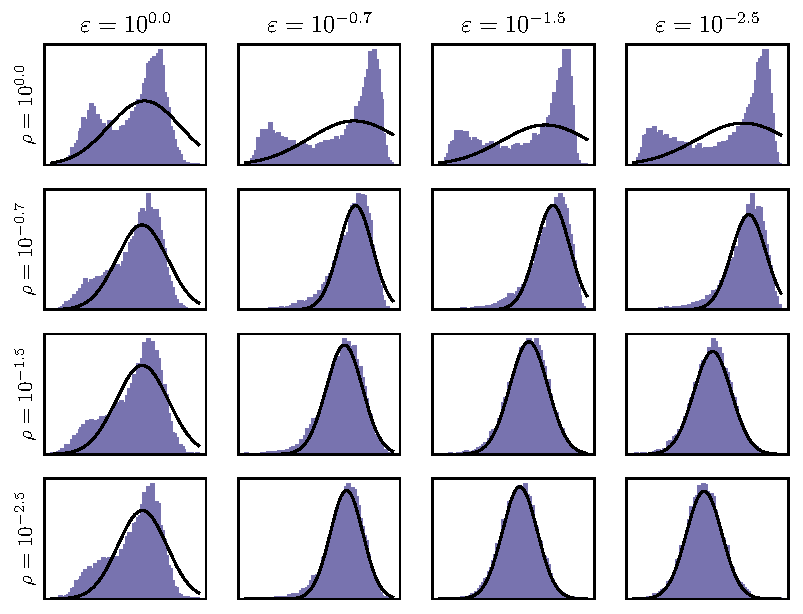
\includegraphics[width=\textwidth]{chp04_paper_numerics/figures/sine/selected_hists.pdf}
		\caption{Histograms of stochastic samples of \cref{eqn:sine_sde}, subject to the Gaussian initial condition \cref{eqn:num_gauss_init}, for varying initial uncertainty scale \(\rho\) and ongoing uncertainty scale \(\epsilon\).
			The distribution of the corresponding solution \cref{eqn:num_linear_sol} to the linearised equation is overlaid in black.}
		\label{fig:sine_hists}
	\end{center}
\end{figure}

In \Cref{fig:sine_hists}, we show histograms of \(N = 10000\) samples of the solution to nonlinear SDE \cref{eqn:sine_sde} and the corresponding probability density function of the linearised solution \cref{eqn:num_linear_sol}, for different combinations of \(\epsilon\) and \(\rho\).
Even when the ongoing noise is small, the nonlinearity of the drift term means that a large initial uncertainty results in a non-Gaussian distribution.
However, in situations where both the initial and ongoing uncertainties are small, the Gaussian solution to the linearised equation provides a reasonable approximation.
In the limit of both small initial (\(\rho \to 0\)) and small ongoing (\(\epsilon \to 0\)) uncertainty (towards the bottom right), we see that the distribution of the samples approach the Gaussian density of the linearisation solution, matching the understanding that the linearisation approximation is ``reasonable'' for small noise regimes.

Since the drift term is nonlinear and the noise is additive in \cref{eqn:sine_sde}, the bound predicted by \Cref{thm:main} has the form
\[
	\avg{\norm{y_t^{(\epsilon)} - l_t^{(\epsilon)}}^r} \leq D_1\!\left(r,t, K_{\nabla u}, K_\sigma\right)\epsilon^{2r} + M_{2r}D_2\!\left(r,t, K_{\nabla u}\right)\rho^{2r}.
\]
where we have taken \(K_{\nabla\nabla u} = 1\) and \(K_{\nabla\sigma} = 0\).
To numerically validate this bound under the Gaussian initial condition \cref{eqn:num_gauss_init}, define for \(r \geq 1\) the error measure
\begin{equation}
	E_r\!\left(\epsilon, \rho\right) \coloneqq \frac{1}{N}\sum_{i=1}^N{\norm{\hat{y}_{i}^{(\epsilon)} - \hat{l}_i^{(\epsilon)}}^r},
	\label{eqn:strong_err_mc_estimate}
\end{equation}
which is a Monte-Carlo estimator of the right-hand side of \cref{eqn:main_ineq}, where \(\hat{y}_1^{(\epsilon)},\dotsc, \hat{y}_N^{(\epsilon)}\) and \(\hat{l}_1^{(\epsilon)},\dotsc, \hat{l}_N^{(\epsilon)}\) are \(N\) numerical samples of the solutions to SDE \cref{eqn:sde_y} and the linearisation \cref{eqn:linear_sde_inform} respectively.

We directly validate the \emph{form} of the error bound (as a function of \(\epsilon\) and \(\rho\)) in \Cref{fig:sine_delta_eps_lines}, by computing \(E_1\) using samples for each pair of \(\epsilon\) and \(\rho\) values.
In \Cref{fig:sine_eps_lines}, we demonstrate the relationship between \(E_1\) and the ongoing uncertainty \(\epsilon\) for several different fixed values of \(\rho\), each corresponding to a different colour.
A least squares estimate of a line of best fit of the form \(E_1 = \beta_0 + \beta_1 \epsilon^2 \), for fixed coefficients \(\beta_0\) and \(\beta_1\), is fitted to the observed errors (in untransformed space) to verify the scaling of our bound in \Cref{thm:main}.
We see that the line of best fit accurately matches the observed values of \(E_1\), verifying that \(E_1\) is in fact scaling with \(\epsilon^2\) as predicted.
\Cref{fig:sine_delta_lines} provides a similar demonstration between \(E_1\) and the initial uncertainty \(\rho\), where now each colour corresponds to a different fixed value of \(\epsilon\).
We again fit lines of the form \(E_1 = \beta_0 + \beta_1 \rho^2\) to verify the scaling of the bound, and see that the lines match the observed values of \(E_2\).
Thus, we have also validated that \(E_1\) scales with \(\rho^2\), as expected from \Cref{thm:main}.

\begin{figure}
	\begin{center}
		\begin{subfigure}{\textwidth}
			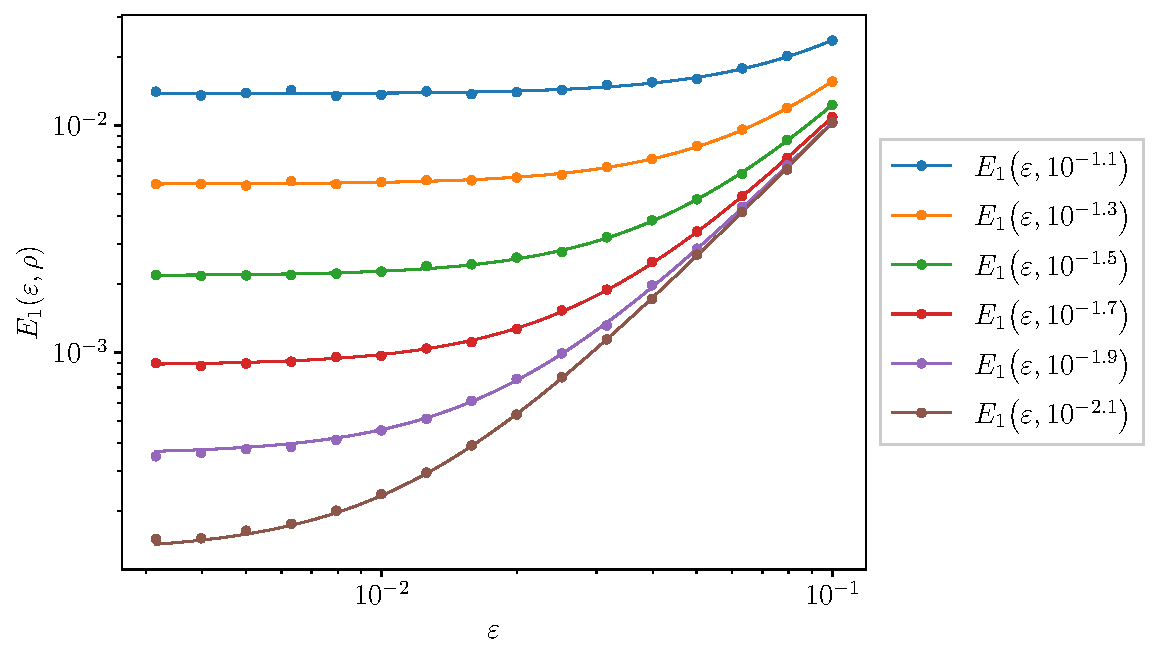
\includegraphics[width=\textwidth]{chp04_paper_numerics/figures/sine/str_err_eps_r_1.0_log.pdf}
			\caption{Estimates of the strong error (with \(r = 1\)) in linearising \cref{eqn:sine_sde} with \cref{eqn:sine_linear}, for varying ongoing uncertainty parameter \(\epsilon\).
				Each colour corresponds to a different value of the initial uncertainty parameter \(\rho\).
				A (least squares) line of best fit of the form \(\beta_0 + \beta_1 \epsilon^2\) is included in the corresponding colour.}
			\label{fig:sine_eps_lines}
		\end{subfigure}
		\begin{subfigure}{\textwidth}
			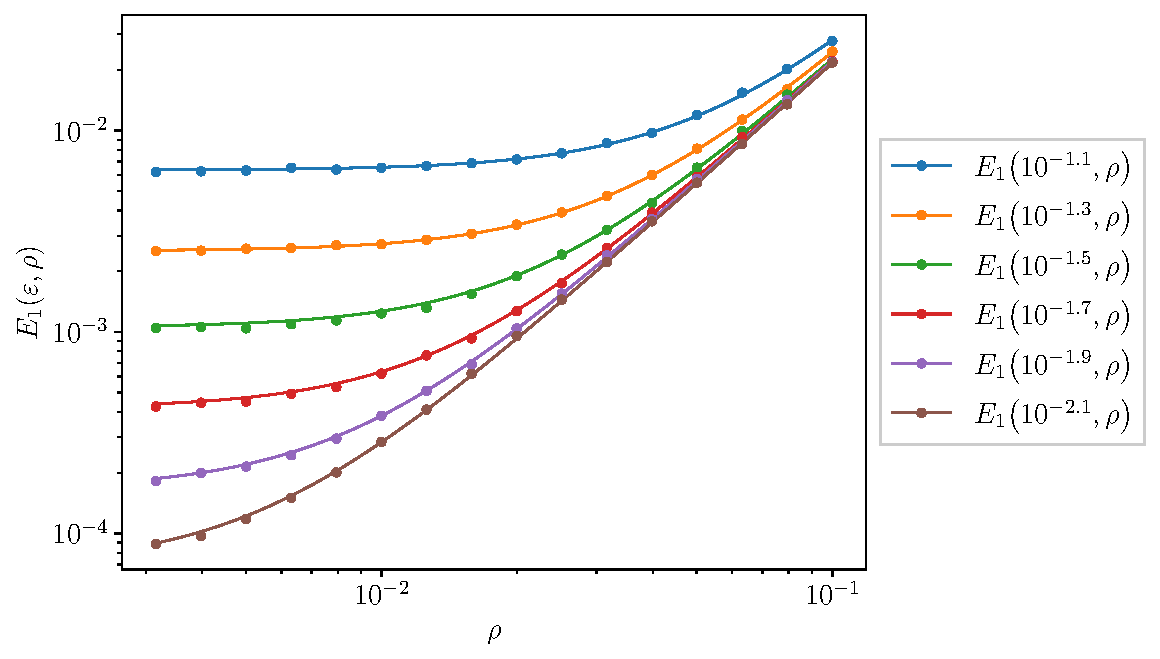
\includegraphics[width=\textwidth]{chp04_paper_numerics/figures/sine/str_err_rho_r_1.0_log.pdf}
			\caption{Estimates of the strong error (with \(r = 1\)) for varying initial uncertainty parameter \(\rho\).
				Each colour corresponds to a different value of the ongoing uncertainty parameter \(\epsilon\).
				A (least squares) line of best fit of the form \(\beta_0 + \beta_1 \rho^2\) is included in the corresponding colour.}
			\label{fig:sine_delta_lines}
		\end{subfigure}
		\caption{Validation of the theoretical bound predicted by \Cref{thm:main}, when \(r = 1\), on numerical realisations of the solution to the 1D example \cref{eqn:sine_sde}.}
		\label{fig:sine_delta_eps_lines}
	\end{center}
\end{figure}

\subsection{Linear dynamics, multiplicative noise}\label{sec:numerics_multiplicative}
Now consider the following SDE with multiplicative noise in 1D;
\begin{equation}
	\dif y_t^{(\epsilon)} = \frac12 y_t^{(\epsilon)}\dif t + \varepsilon \cos\!\left(y_t^{(\epsilon)}\right) \dif W_t.
	\label{eqn:1d_mult}
\end{equation}
The corresponding deterministic system is linear and has solution
\begin{equation}
	F_0^t\!\left(x_0\right) = \exp\!\left(\frac{t}{2}\right) x_0,
	\label{eqn:1d_mult_det_sol}
\end{equation}
with additional details provided in the supplementary materials.
As with the previous example in \Cref{sec:numerics_nonlinear}, we take the Gaussian initial condition \cref{eqn:num_gauss_init} with variance \(\rho^2\) and linearised \cref{eqn:1d_mult} about the initial mean \(\mu\).
The linearised equation is then
\begin{equation}
	\dif l_t^{(\epsilon)} = \frac12 l_t^{(\epsilon)}\dif t + \epsilon \cos\!\left(\exp\left(\frac{t}{2}\right)\mu\right) \dif W_t, \quad l_0^{(\epsilon)} \sim \Gauss{\mu, \rho^2},
	\label{eqn:1d_mult_linear}
\end{equation}
with Gaussian solution \cref{eqn:num_linear_sol}.
We take the initial point \(\mu = 2\) and consider the solutions at time \(t = 1\).
To generate numerical realisations of the solutions to \cref{eqn:1d_mult} and \cref{eqn:1d_mult_linear} with the same realisations of \(W_t\), we use the same set-up as in the previous example.

In \Cref{fig:sine_hists}, we show histograms of \(N = 10000\) samples of the multiplicative noise SDE \cref{eqn:1d_mult} and the corresponding probability density function of the linearised solution, for different combinations of \(\epsilon\) and \(\rho\).
We again see that in the limit of both small initial and small ongoing uncertainty (towards the bottom right), we see that the distribution of the samples approach the Gaussian density of the linearisation solution.

\begin{figure}
	\begin{center}
		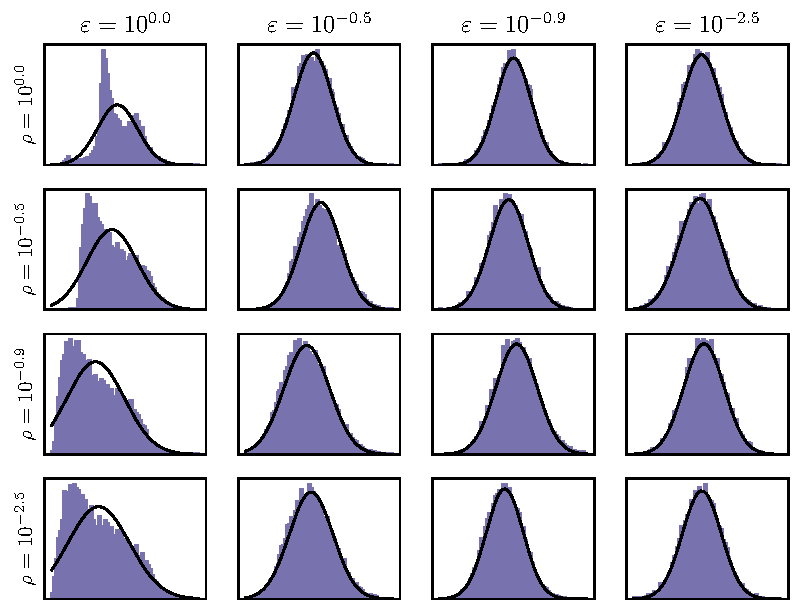
\includegraphics[width=\textwidth]{chp04_paper_numerics/figures/multiplicative/selected_hists.pdf}
		\caption{The same arrangement as \Cref{fig:sine_hists}, but for the 1D multiplicative noise SDE \cref{eqn:1d_mult}.}
		\label{fig:1d_mult_hists}
	\end{center}
\end{figure}

Since the drift term is linear and the noise multiplicative in \cref{eqn:1d_mult}, the bound predicted by \Cref{thm:main} has the form
\[
	\avg{\norm{y_t^{(\epsilon)} - l_t^{(\epsilon)}}^r} \leq D_1\!\left(r,t, K_{\nabla u}, K_\sigma\right)\epsilon^{2r} + M_{r}D_3\!\left(r,t, K_{\nabla u}\right)\epsilon^r\rho^{r},
\]
where we have \(K_{\nabla\nabla u} = 0\) and \(K_{\nabla\sigma} = 1\).
In \Cref{fig:multiplicative_delta_eps_lines}, we again validate the form of this bound (for \(r = 1\); results for additional values of \(r\) are provided in the supplementary material) by approximating the left-hand side with \(E_1\) computed from realisations of the solution to \cref{eqn:1d_mult} and the linearisation \cref{eqn:1d_mult_linear}.
For each fixed value of the initial uncertainty \(\rho\), in \Cref{fig:multiplicative_eps_lines}, we fit a line of best fit of the form \(\beta_1 \epsilon + \beta_2 \epsilon^2\) to validate that the strong error scales as predicted.
Similarly, in \Cref{fig:multiplicative_eps_lines} we fit a line of best fit of the form \(\beta_0 + \beta_1 \rho\) and confirm that the linearisation error follows this scaling.

\begin{figure}
	\begin{center}
		\begin{subfigure}{\textwidth}
			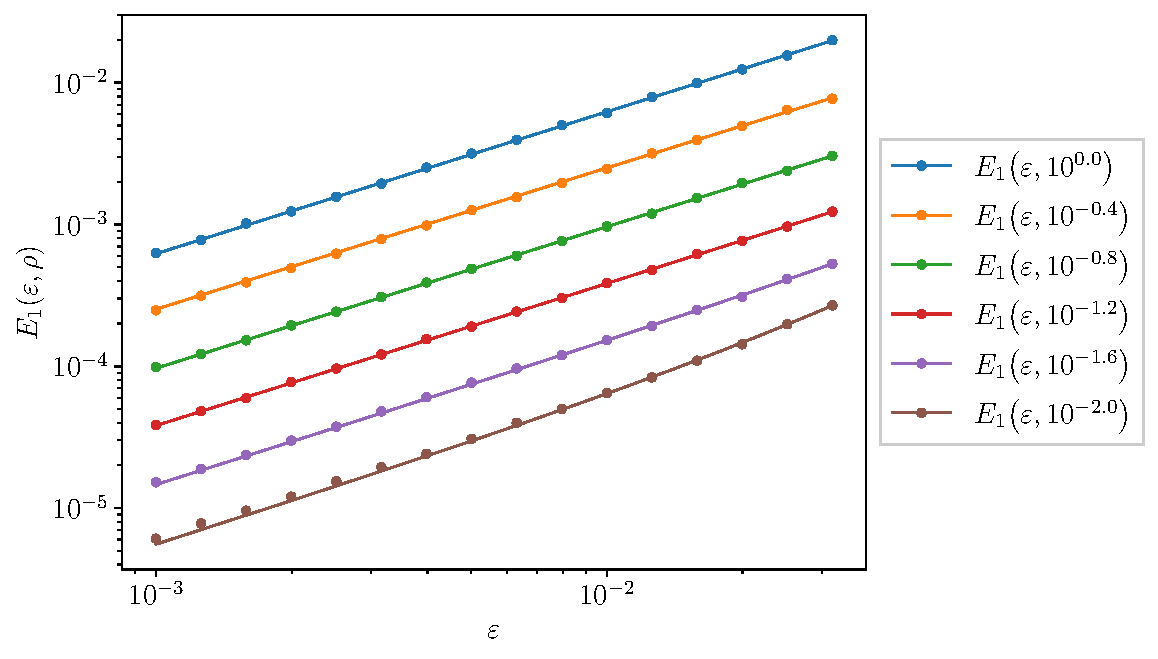
\includegraphics[width=\textwidth]{chp04_paper_numerics/figures/multiplicative/str_err_eps_r_1.0_log.pdf}
			\caption{Estimates of the strong order (with \(r = 1\)) for varying ongoing uncertainty parameter \(\epsilon\).
				Each colour corresponds to a different value of the initial uncertainty parameter \(\rho\).
				A (least squares) line of best fit of the form \(\beta_1 \epsilon + \beta_2 \epsilon^2\) is included in the corresponding colour.}
			\label{fig:multiplicative_eps_lines}
		\end{subfigure}
		\begin{subfigure}{\textwidth}
			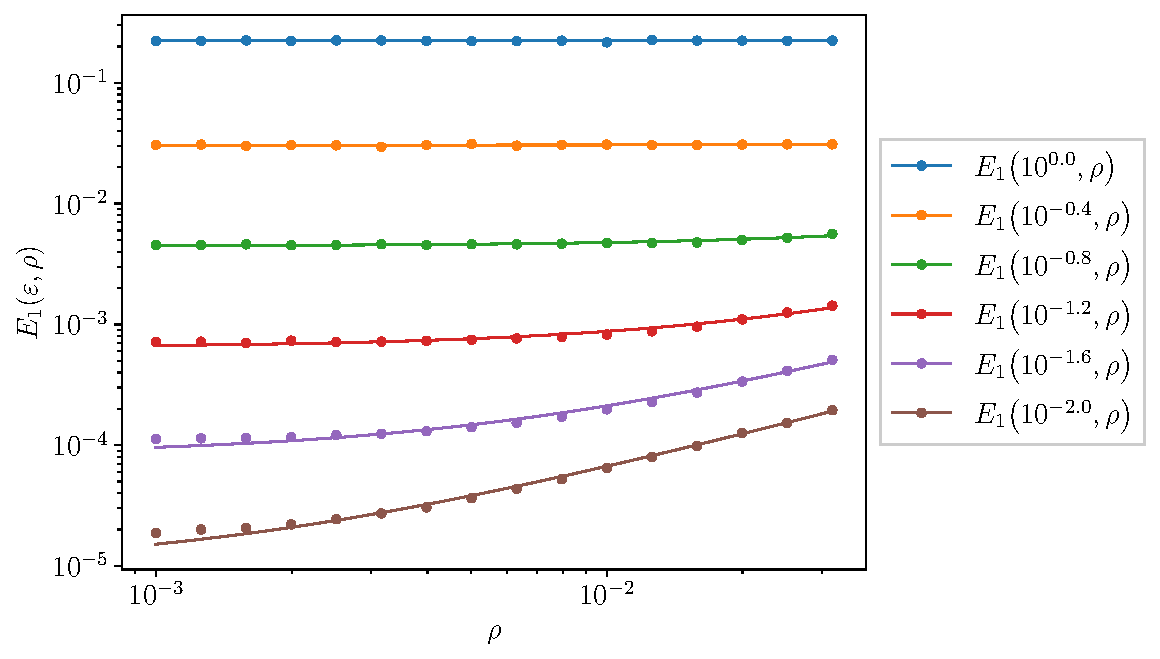
\includegraphics[width=\textwidth]{chp04_paper_numerics/figures/multiplicative/str_err_rho_r_1.0_log.pdf}
			\caption{Estimates of the strong order (with \(r = 1\)) for varying initial uncertainty parameter \(\rho\).
				Each colour corresponds to a different value of the ongoing uncertainty parameter \(\epsilon\).
				A (least squares) line of best fit of the form \(\beta_0 + \beta_1 \rho\) is included in the corresponding colour.}
			\label{fig:multiplicative_delta_lines}
		\end{subfigure}
		\caption{Validation of the theoretical bound predicted by \Cref{thm:main}, when \(r = 1\), on numerical realisations of the solution to the 1D example \cref{eqn:1d_mult}.}
		\label{fig:multiplicative_delta_eps_lines}
	\end{center}
\end{figure}

\subsection{Fixed initial condition}\label{sec:numerics_2d}
In this example, we consider a two-dimensional model and a fixed initial condition, to validate the results presented in \Cref{sec:theory_fixed}.
Following the example in Chapter 5 of \citet{SamelsonWiggins_2006_LagrangianTransportGeophysical}, we consider an unsteady meandering jet in two dimensions, which may serve as an idealised model of geophysical Rossby waves \citep{Pierrehumbert_1991_ChaoticMixingTracer}.
The velocity field for \(y \equiv \left(y_1, y_2\right)^{\T}\) is given by
\begin{equation}
	u\!\left(y, t\right) = \begin{bmatrix}
		c - A\sin\!\left(Ky_1\right)\cos\!\left(y_2\right) + \oldepsilon_{\mathrm{mj}} l_1\sin\!\left(k_1\left(y_1 - c_1 t\right)\right)\cos\!\left(l_1 y_2\right) \\
		AK\cos\!\left(Ky_1\right)\sin\!\left(y_2\right) + \oldepsilon_{\mathrm{mj}} k_1\cos\!\left(k_1\left(y_1 - c_1t\right)\right)\sin\!\left(l_1 y_2\right)
	\end{bmatrix}.
	\label{eqn:jet_ex}
\end{equation}
The velocity field describes a kinematic travelling wave with deterministic oscillatory perturbations in a co-moving frame.
Here, \(A\) is the amplitude and \(c\) is the phase speed of the primary wave, and \(K\) is the wavenumber in the \(y_1\)-direction.
The oscillatory perturbation has amplitude \(\oldepsilon_{\mathrm{mj}}\), phase speed \(c_1\) (in the co-moving frame), and wavenumbers \(k_1\) and \(l_1\) in the \(y_1\)- and \(y_2\)-directions respectively.
Throughout, we take the parameter values \(c = 0.5\), \(A = 1\), \(K = 4\), \(l_1 = 2\), \(k_1 = 1\), \(c_1 = \pi\), and \(\oldepsilon_{\mathrm{mj}} = 0.3\).
For these values, the flow consists of a meandering jet with vortex structures within the meanders, and a chaotic zone which influences the fluid transfer between the jet and the vortices.

We introduce multiplicative noise by considering stochastic perturbations to the phase speed \(c\) and the primary amplitude \(A\), which we model with the respective components of a \(2\)-dimensional Wiener process \(W_t = \left(W_t^{(1)}, W_t^{(2)}\right)^{\T}\).
Then, we specify the diffusion term as
\begin{equation}
	\sigma\!\left(y,t\right) = \begin{bmatrix}
		1 & \sin\!\left(Ky_1\right)\cos\!\left(y_2\right)  \\
		0 & K\cos\!\left(Ky_1\right)\sin\!\left(y_2\right)
	\end{bmatrix}.
	\label{eqn:jet_ex_sigma}
\end{equation}


We consider the fixed initial condition \(x_0 = \left(0, 1\right)\) and the prediction of the model at time \(t = 1\).
We then consider a linearisation of the SDE about the deterministic trajectory \(F_0^t\!\left(x_0\right)\), where \(F_0^t\) is the deterministic flow map corresponding to the vector field \cref{eqn:jet_ex}.
To compute the Gaussian distribution \cref{eqn:linear_gauss_sol} of the linearised solution, we again solve \cref{eqn:pi_ode} numerically with initial condition \(\Sigma_0^t\!\left(x_0\right) = O\).
Specifically, \cref{eqn:pi_ode} is solved jointly with the deterministic state equation \cref{eqn:ode_det} using the hybrid method proposed by \citet{Mazzoni_2008_ComputationalAspectsContinuous}.
This hybrid method combines a Taylor-Heun approximation with a Gauss-Legendre one and ensures that the numerical solution of the covariance equation is symmetric and positive semi-definite while maintaining both accuracy and computational efficiency.


\Cref{fig:y_hists} shows the resulting simulations of \(y_t^{(\epsilon)}\) for four different values of \(\epsilon\).
The realisations are binned as a histogram and bin counts are normalised, to provide an empirical estimate of the probability density function of \(y_t^{(\epsilon)}\).
Superimposed (in solid black) are the first, second and third standard-deviation contours of the probability density function of the Gaussian distribution that solves the linearised equation.
The first three standard-deviation levels of the \(2\times 2\) sample covariance matrix of the realisations of \(y_t^{(\epsilon)}\), are also overlaid (in dashed blue).
As \(\epsilon\) decreases towards \(0\), the samples increasingly resemble a Gaussian distribution, and both the mean and covariance coincide with the corresponding limits.

\begin{figure}
	\begin{center}
		\begin{subfigure}{0.49\textwidth}
			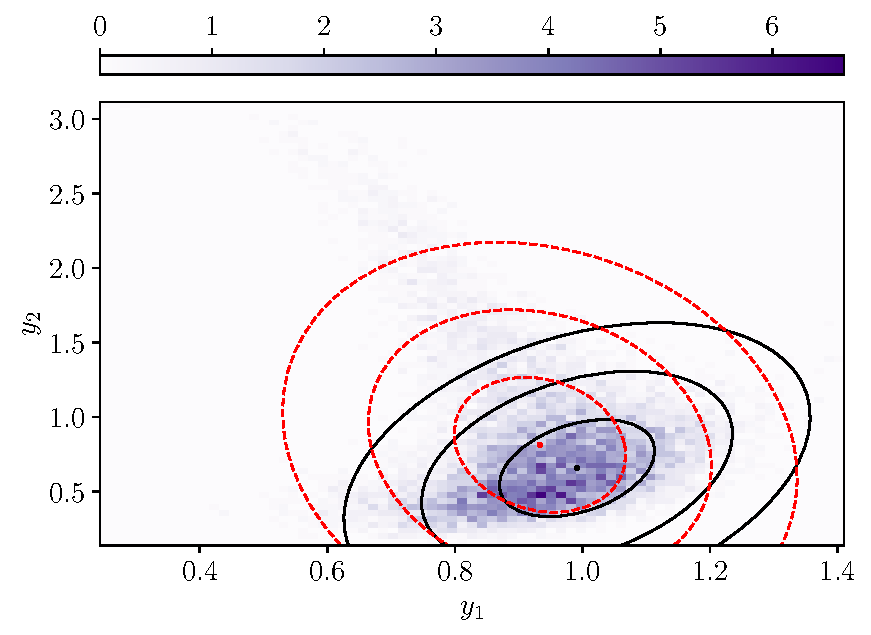
\includegraphics[width=\textwidth]{chp04_paper_numerics/figures/rossby/hist_0.1.pdf}
			\caption{\(\epsilon = 10^{-1}\)}
			\label{fig:y_hists_a}
		\end{subfigure}
		\begin{subfigure}{0.49\textwidth}
			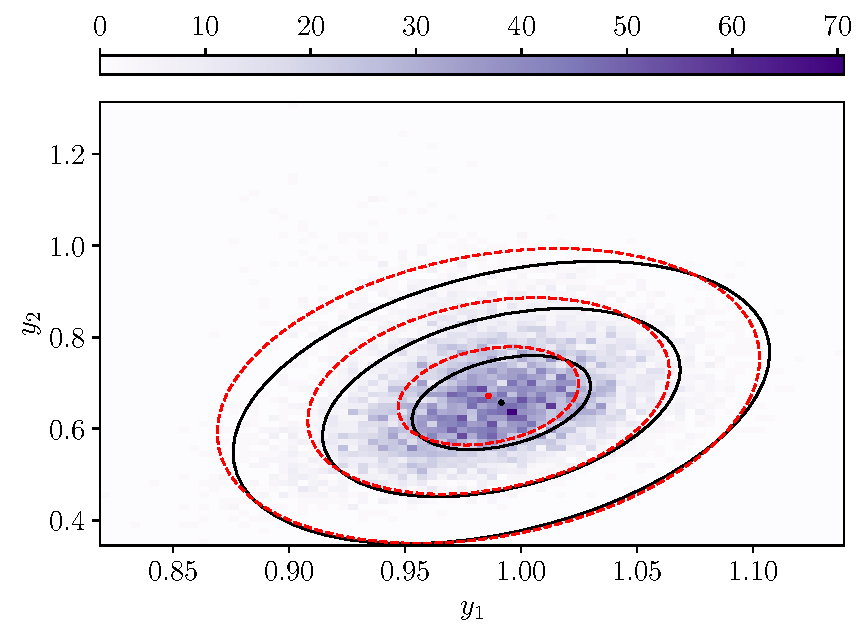
\includegraphics[width=\textwidth]{chp04_paper_numerics/figures/rossby/hist_0.03162277660168379.pdf}
			\caption{\(\epsilon = 10^{-1.5}\)}
			\label{fig:y_hists_b}
		\end{subfigure}
		\begin{subfigure}{0.49\textwidth}
			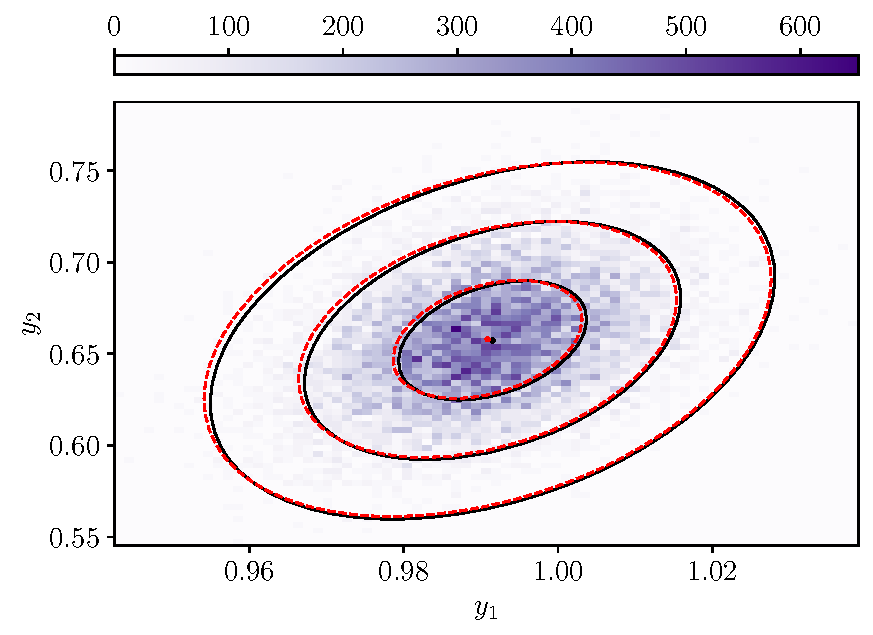
\includegraphics[width=\textwidth]{chp04_paper_numerics/figures/rossby/hist_0.010000000000000002.pdf}
			\caption{\(\epsilon = 10^{-2}\)}
			\label{fig:y_hists_c}
		\end{subfigure}
		\begin{subfigure}{0.49\textwidth}
			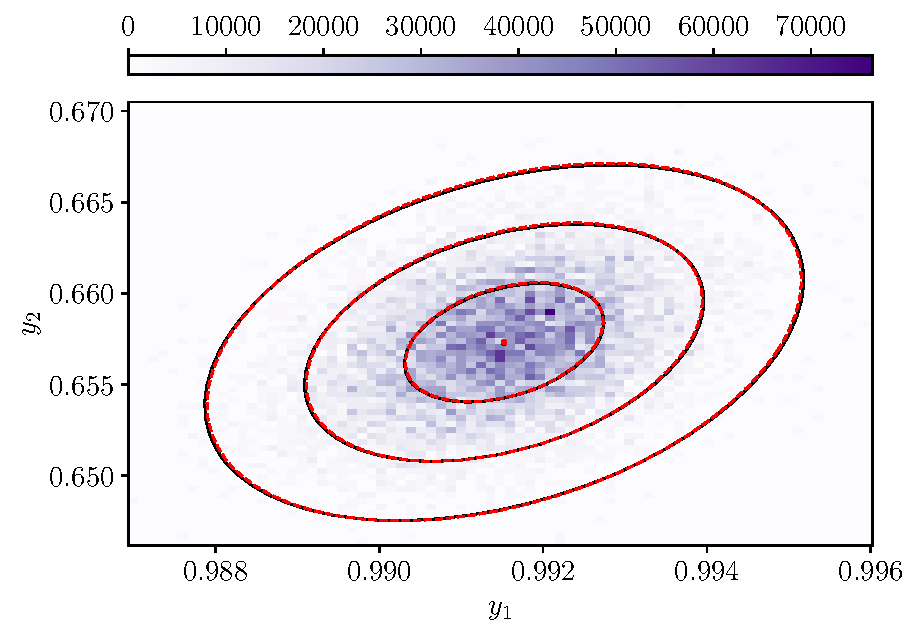
\includegraphics[width=\textwidth]{chp04_paper_numerics/figures/rossby/hist_0.001.pdf}
			\caption{\(\epsilon = 10^{-3}\)}
			\label{fig:y_hists_d}
		\end{subfigure}
		\caption{Histograms of \(y_t^{(\epsilon)}\) from direct simulation of the SDE with drift \cref{eqn:jet_ex} and diffusivity \cref{eqn:jet_ex_sigma} subject to the fixed initial condition, for four different \(\epsilon\) values.
		Overlaid in black are contours of the Gaussian solution \cref{eqn:linear_gauss_sol} of the linearised SDE \cref{eqn:linear_sde_inform}, which correspond to the first three standard deviation levels centred at the mean \(F_0^t(x)\).
		In dashed blue are corresponding contours computed from the sample covariance matrix of the realisations.
		}
		\label{fig:y_hists}
	\end{center}
\end{figure}

For a fixed initial condition, \cref{eqn:main_ineq} predicts that the expected distance between the original SDE solution and that of a linearisation satisfies
\[
	\avg{\norm{y_t^{(\epsilon)} - l_t^{(\epsilon)}}^r} \leq \left(K_{\nabla\nabla u} + K_{\nabla\sigma}\right)D_1\!\left(r,t, K_{\nabla u}, K_\sigma\right)\epsilon^{2r}.
\]
To numerically estimate the left-hand side of \cref{eqn:main_ineq}, we again use a Monte-Carlo estimator;
\[
	E_r\!\left(\epsilon\right) \coloneqq \frac{1}{N}\sum_{i=1}^N{\norm{\hat{y}_i^{(\epsilon)} - \hat{l}_i^{(\epsilon)}}^r}.
\]
For \(r = 1,2,3,4\), \(E_r\!\left(\epsilon\right)\) is shown (in a logarithmic scale) for decreasing values of \(\epsilon\) in \Cref{fig:gamma_z_valid}.
\Cref{thm:main} predicts that \(\log_{10}\left(E_r\!\left(\epsilon\right)\right)\) should decay linearly with a slope greater than \(2r\) as \(\epsilon\) decreases to zero.
The least squares lines of best fit for each value of \(r\) in \Cref{fig:gamma_z_valid} show this behaviour, and are therefore consistent with \Cref{thm:main}.

\begin{figure}
	\begin{center}
		\begin{subfigure}{0.49\textwidth}
			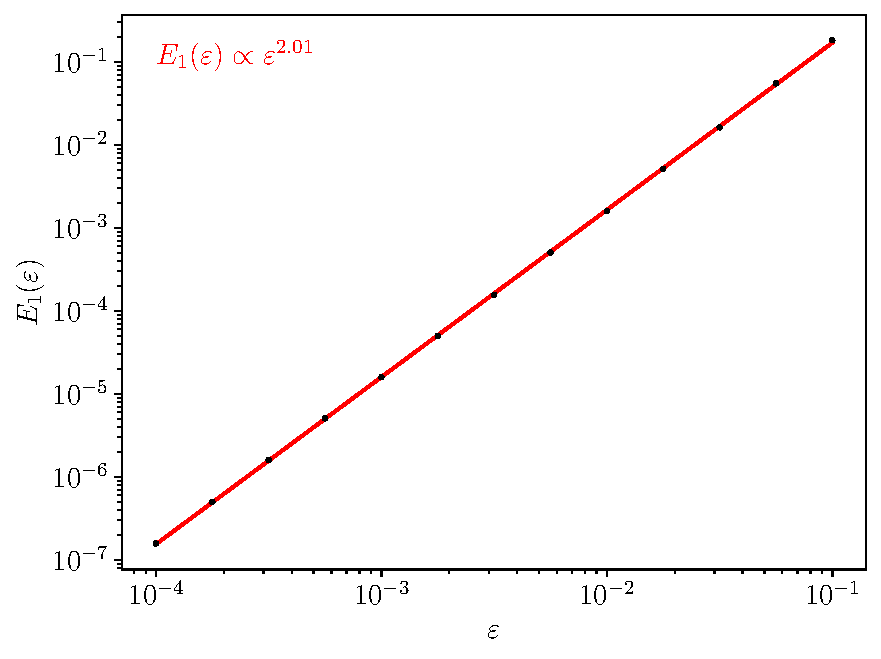
\includegraphics[width=\textwidth]{chp04_paper_numerics/figures/rossby/str_err_r_1.0.pdf}
			\caption{\(r = 1\) (mean)}
			\label{fig:gamma_z_valid_1}
		\end{subfigure}
		\begin{subfigure}{0.49\textwidth}
			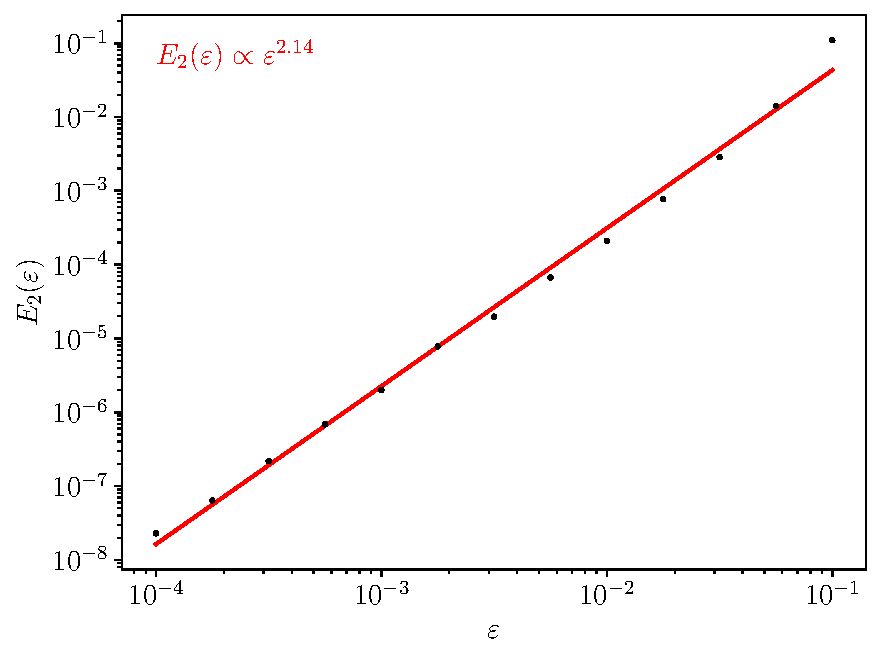
\includegraphics[width=\textwidth]{chp04_paper_numerics/figures/rossby/str_err_r_2.0.pdf}
			\caption{\(r = 2\) (variance)}
			\label{fig:gamma_z_valid_2}
		\end{subfigure}
		\begin{subfigure}{0.49\textwidth}
			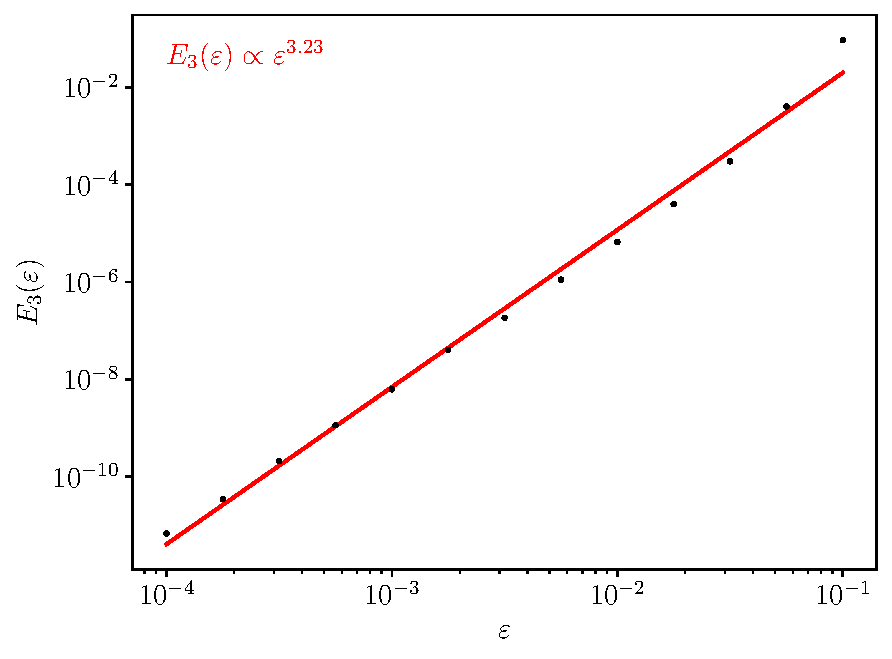
\includegraphics[width=\textwidth]{chp04_paper_numerics/figures/rossby/str_err_r_3.0.pdf}
			\caption{\(r = 3\) (skewness)}
			\label{fig:gamma_z_valid_3}
		\end{subfigure}
		\begin{subfigure}{0.49\textwidth}
			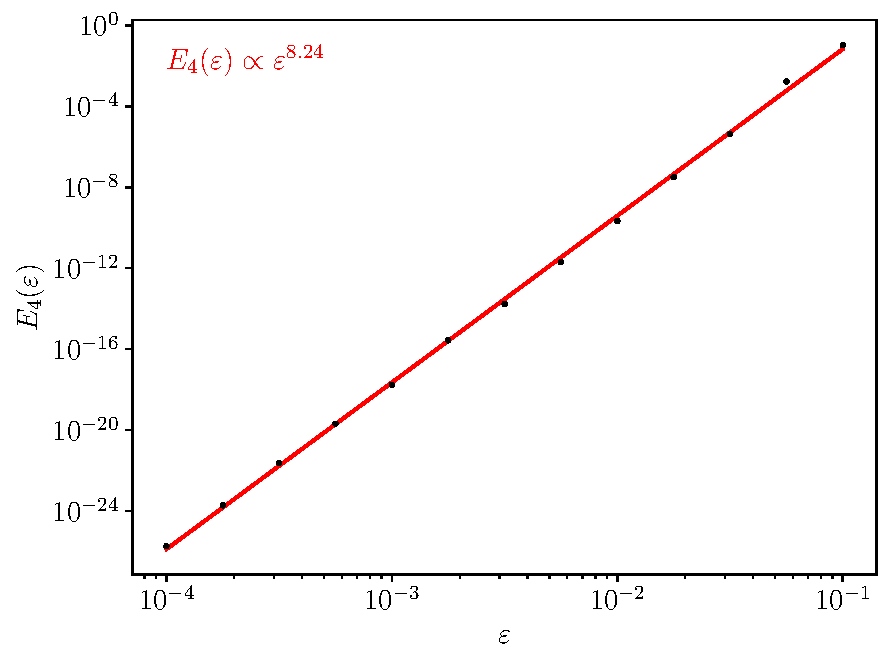
\includegraphics[width=\textwidth]{chp04_paper_numerics/figures/rossby/str_err_r_4.0.pdf}
			\caption{\(r = 4\) (kurtosis)}
			\label{fig:gamma_z_valid_4}
		\end{subfigure}

		\caption{Validation of \Cref{thm:main}, by plotting the sample \(r\)th raw moment distance (the error metric \(E_r(\epsilon)\)) between \(10000\) realisations of the meandering jet SDE and a corresponding linearisation, for decreasing values of \(\epsilon\).
			A line of best fit (in red) is placed on each, and the resulting slope indicated.}
		\label{fig:gamma_z_valid}
	\end{center}
\end{figure}


\section{Computing stochastic sensitivity} \label{sec:comput_s2}
In this section, we illustrate the computability of stochastic sensitivity as described in \Cref{thm:s2_calculation}.

\subsection{In 2-dimensions}\label{sec:compute_s2_2d}

\begin{figure}
	\begin{center}
		\begin{subfigure}{\textwidth}
			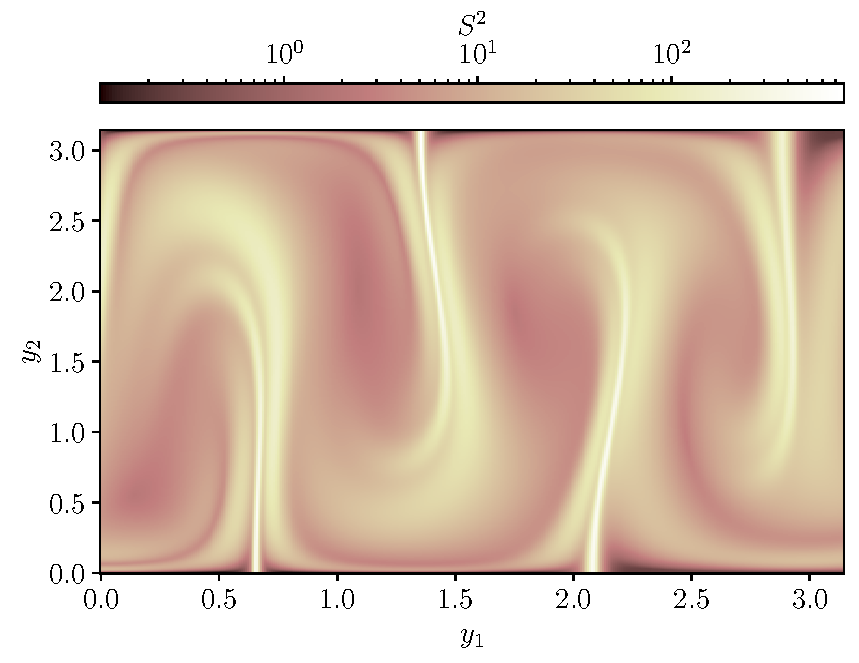
\includegraphics[width=0.49\textwidth]{chp04_paper_numerics/figures/rossby/S2_zero_0.3}
			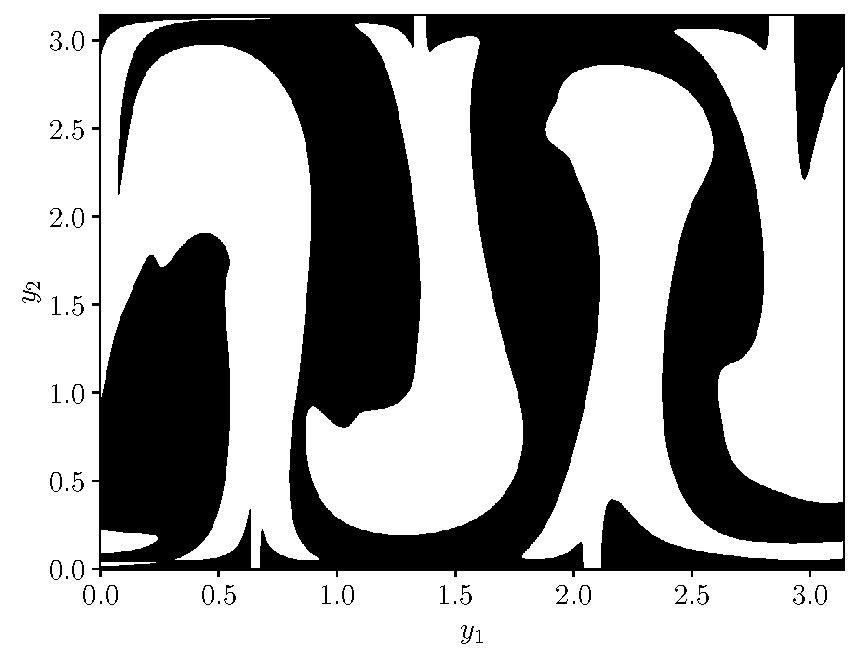
\includegraphics[width=0.49\textwidth]{chp04_paper_numerics/figures/rossby/S2_robust_0.3}
			\caption{\(\oldepsilon_{\mathrm{mj}} = 0.3\)}
			\label{fig:s2_field_0.3}
		\end{subfigure}
		\begin{subfigure}{\textwidth}
			\includegraphics[width=0.49\textwidth]{chp04_paper_numerics/figures/rossby/s2_zero_1.0}
			\includegraphics[width=0.49\textwidth]{chp04_paper_numerics/figures/rossby/s2_robust_1.0}
			\caption{\(\oldepsilon_{\mathrm{mj}} = 1.0\)}
			\label{fig:s2_field_1.0}
		\end{subfigure}
		\caption{(Left) The \(S^2\) field of the meandering jet flow \cref{eqn:jet_ex} over the time interval \([0,1]\), for two different sets of parameters with qualitatively different behaviour.
			The \(S^2\) value for each initial condition is computed directly as the operator norm of the covariance matrix \(\Sigma_0^1\!\left(x_0\right)\), as per \cref{eqn:s2_calculation}.
			(Right) Robust sets extracted from the stochastic sensitivity fields, by taking the initial conditions with a stochastic sensitivity value about a threshold of \(10\).}
		\label{fig:ex_jet_s2_field}
	\end{center}
\end{figure}

We again consider the meandering jet \cref{eqn:jet_ex} with multiplicative noise described by \cref{eqn:jet_ex_sigma}.
We take the same choice of parameters as in \cref{sec:numerics_2d}, except for the perturbation amplitude \(\oldepsilon_{\mathrm{mj}}\) which is varied to obtain qualitatively different behaviour in the system.
For each initial condition in a \(400 \times 400\) uniform grid on \(\left[0, \pi\right] \times \left[0, \pi\right]\), the \(S^2\) value is calculated using \cref{eqn:s2_calculation}.
\Cref{fig:ex_jet_s2_field} shows the resulting \(S^2\) field from time \(0\) to \(t = 1\), for two different values of \(\oldepsilon_{\mathrm{mj}}\).
We also extract robust sets from each stochastic sensitivity field, by highlighting in cyan on the right side of \Cref{fig:ex_jet_s2_field} those initial conditions with a stochastic sensitivity value less than the specified threshold of 10.
When \(\oldepsilon_{\mathrm{mj}} = 0.3\) (\Cref{fig:s2_field_0.3}), the \(S^2\) field is largest in the elongated gyre regions outside of the meandering jet, where the flow exhibits chaotic behaviour \citep{Pierrehumbert_1991_ChaoticMixingTracer} and we accordingly expect larger uncertainty due to the model dynamics.
As a region of small \(S^2\) value, the meandering jet emerges as a robust set, consisting of initial points whose eventual fate is significantly more certain than in other regions.
When \(\oldepsilon_{\mathrm{mj}} = 1.0\) (\Cref{fig:s2_field_1.0}), the deterministic flow is dominated by oscillatory perturbation, which further increases the chaotic nature of the solving trajectories and the boundaries between the gyres and the meandering jet are no longer distinguishable \citep{Crocker_2021_LagrangianCoherentData}.
Rotational eddies begin to dominate the flow and we see this reflected in the stochastic sensitivity field in \Cref{fig:s2_field_1.0}: the eddies exhibit a smaller stochastic sensitivity, as even under stochasticity trajectories are inclined to remain within them.
The resulting robust sets highlight these eddies.\lb{Don't love this analysis, but almost there. Reconsider on next read through.}

% \begin{figure}
% 	\begin{center}
% 		\begin{subfigure}{0.49\textwidth}
% 			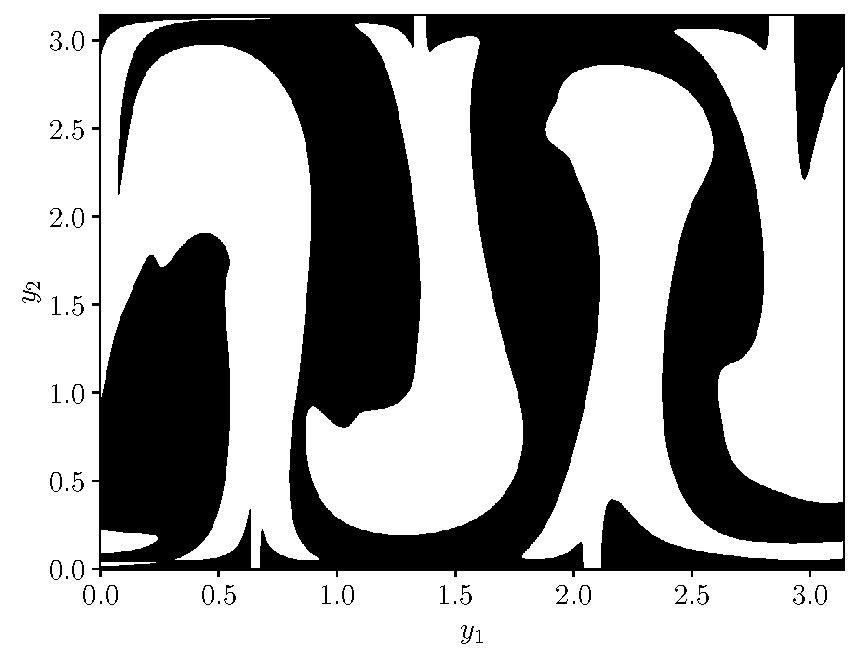
\includegraphics[width=\textwidth]{chp04_paper_numerics/figures/rossby/S2_robust_0.3.pdf}
% 			\caption{\(\oldepsilon_{\mathrm{mj}} = 0.3\), \(R = 10\)}
% 		\end{subfigure}
% 		\begin{subfigure}{0.49\textwidth}
% 			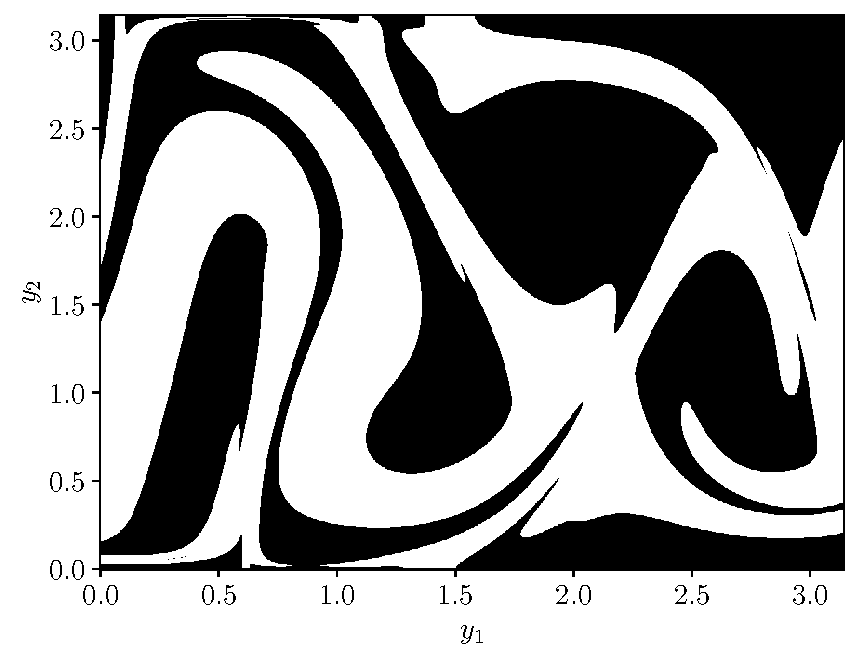
\includegraphics[width=\textwidth]{chp04_paper_numerics/figures/rossby/S2_robust_1.0.pdf}
% 			\caption{\(\oldepsilon_{\mathrm{mj}} = 1.0\), \(R = 10\)}
% 		\end{subfigure}
% 		\caption{Robust sets extracted from the stochastic sensitivity fields in \Cref{fig:ex_jet_s2_field}, by taking the initial conditions with a stochastic sensitivity value above a specified threshold \(R\). }
% \td{Use cyan for robust sets, to be consistent with later results.}
% 		\label{fig:ex_jet_robust}
% 	\end{center}
% \end{figure}

% The stochastic sensitivity field can highlight Lagrangian coherent structures within the flow, by identifying regions of the flow with a relatively small uncertainty, as measured by a \emph{single} number for each initial condition.
% Subsets of the spatial domain corresponding to coherent structures can be extracted, e.g.\ by taking a threshold on \(S^2\) as described in the original work \citep{Balasuriya_2020_StochasticSensitivityComputable}; further examples of coherent structure extraction with stochastic sensitivity on both toy models and real data can be found in \citet{Balasuriya_2020_StochasticSensitivityComputable} and \citet{BadzaEtAl_2023_HowSensitiveAre}.
% Here, we demonstrate the extraction of coherent structures in \Cref{fig:ex_jet_robust} using a threshold of \(R\).
% The resulting subsets of the domain in cyan reflect our conclusions from the stochastic sensitivity field itself; when \(\epsilon_{\mathrm{mj}} = 0.3\) the meandering jet



% \begin{figure}
% 	\begin{center}
% 		\begin{subfigure}{0.49\textwidth}
% 			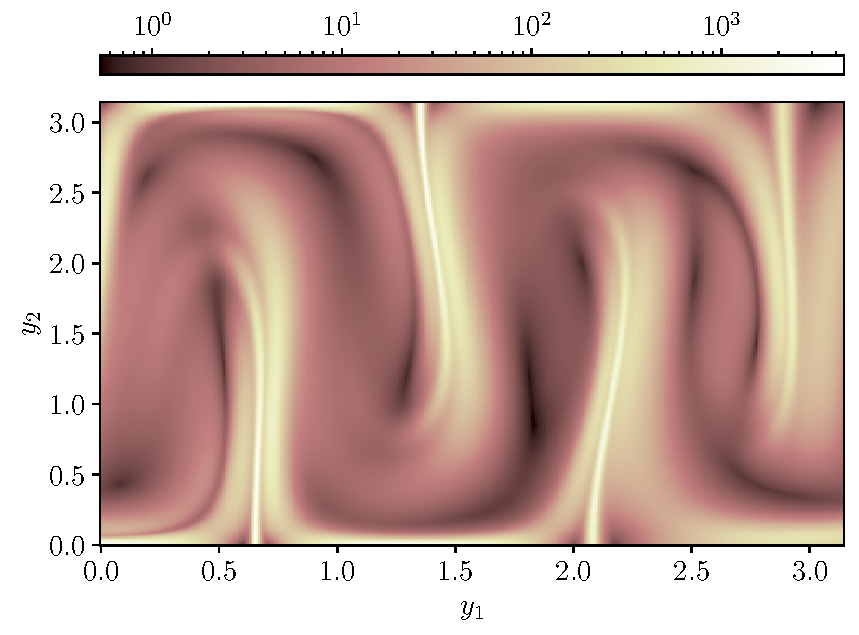
\includegraphics[width=\textwidth]{chp04_paper_numerics/figures/rossby/ftle_0.3.pdf}
% 			\caption{\(\oldepsilon_{\mathrm{mj}} = 0.3\)}
% 		\end{subfigure}
% 		\begin{subfigure}{0.49\textwidth}
% 			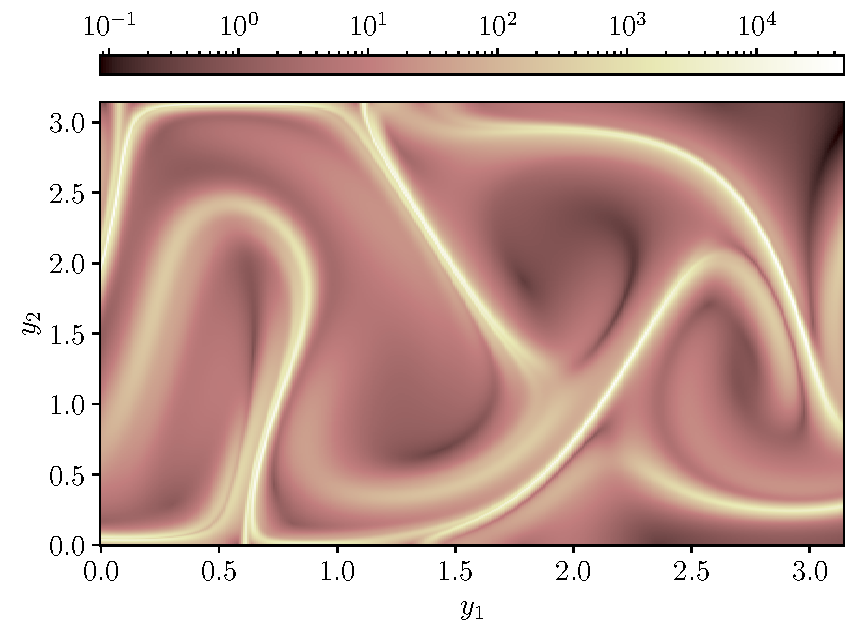
\includegraphics[width=\textwidth]{chp04_paper_numerics/figures/rossby/ftle_1.0.pdf}
% 			\caption{\(\oldepsilon_{\mathrm{mj}} = 1.0\)}
% 		\end{subfigure}
% 		\caption{The finite-time Lyapunov exponent field of the meandering jet flow \cref{eqn:jet_ex} over the time \([0,1]\), for two different values of \(\oldepsilon_{\mathrm{mj}}\).
% 			These fields should be compared with the corresponding stochastic sensitivity fields in \Cref{fig:ex_jet_s2_field}.}
% 	\end{center}
% 	\label{fig:ex_jet_ftle}
% \end{figure}



% In this example, the stochastic sensitivity and FTLE fields show strong similarities, supporting the claims in \Cref{sec:ftle_s2_connection} that stochastic sensitivity can be considered a generalisation of the FTLE.
% The two fields are quantifying different aspects of the flow, however, and so can show differences; such examples are available in \citet{Balasuriya_2020_StochasticSensitivityComputable} (see Figure 3.7) and \citet{BadzaEtAl_2023_HowSensitiveAre} (compare Figures 1 and 5, and Figures 11 and 15).

% To highlight the differences between the stochastic sensitivity field and the finite-time Lyapunov exponent, here we provide a brief and contrived example in which multiplicative noise has a substantial impact on the dynamical behaviour of the system.
% Following the example of \citet{BalasuriyaGottwald_2018_EstimatingStableUnstable}, consider the two-dimensional velocity field
% \begin{equation*}
% 	u\!\left(y, t\right) = \begin{bmatrix}
% 		-4y_1 + y_1^2 \\
% 		3y_2 - y_2^3
% 	\end{bmatrix},
% \end{equation*}
% To introduce multiplicative noise, we take the diffusivity
% \[
% 	\sigma\!\left(y,t\right) = \begin{bmatrix}
% 		1       & 0                                       \\
% 		y_2 - 1 & 3\sin\!\left(2\pi y_1\right)e^{-0.8y_1}
% 	\end{bmatrix},
% \]
% which in particular ensures a non-trivial spatial dependence along the stable manifold of interest.





% \begin{figure}
% 	\begin{center}
% 		\begin{subfigure}{0.49\textwidth}
% 			\includegraphics[width=\textwidth]{chp04_paper_numerics/figures/unstable/ftle.pdf}
% 			\caption{FTLE}
% 			\label{fig:s2_ftle_ftle}
% 		\end{subfigure}
% 		\begin{subfigure}{0.49\textwidth}
% 			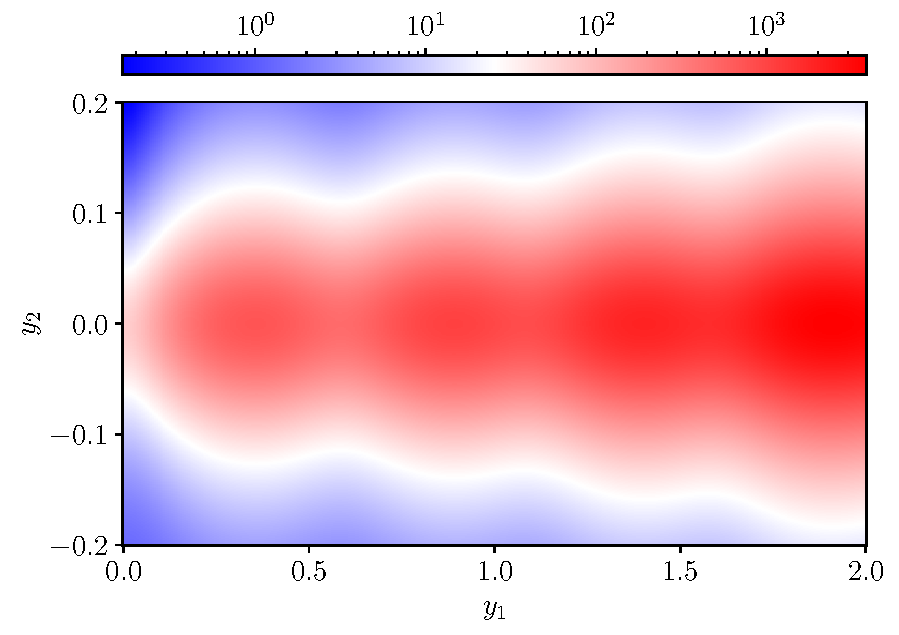
\includegraphics[width=\textwidth]{chp04_paper_numerics/figures/unstable/S2_zero.pdf}
% 			\caption{\(S^2\) with fixed initial condition.}
% 			\label{fig:s2_ftle_ftle}
% 		\end{subfigure}		\begin{subfigure}{0.49\textwidth}
% 			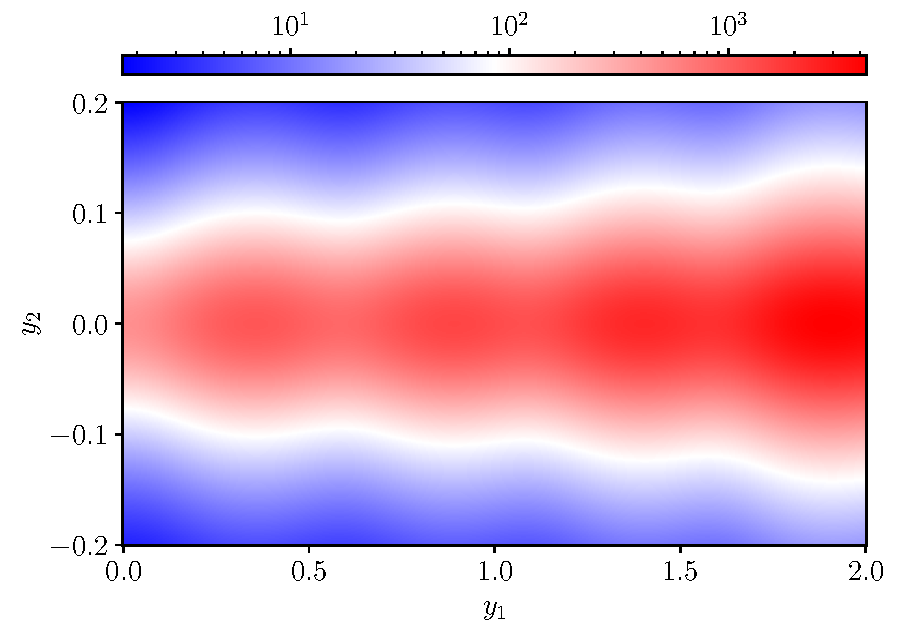
\includegraphics[width=\textwidth]{chp04_paper_numerics/figures/unstable/S2_I.pdf}
% 			\caption{\(S^2\) with standard Gaussian initial condition.}
% 			\label{fig:s2_ftle_ftle}
% 		\end{subfigure}
% 		\caption{The stochastic sensitivity and FTLE-type stretching fields for the two-dimensional}
% 		\label{fig:}
% 	\end{center}
% \end{figure}



%To briefly demonstrate that the stochastic sensitivity field and the resulting robust sets are in fact accounting for uncertainty, we consider a simpler, contrived example.
%We again take the velocity field \eqref{eqn:jet_ex} describing the meandering jet, but now assume that the ongoing stochasticity is 1-dimensional, i.e. \(m = 1\) in the notation of \Cref{ch:linear_theory}, and only acts on the \(y_1\)-component.
%That is, we are considering the stochastic model
%\[
%	\dif \begin{bmatrix}
%		y_1 \\ y_2
%	\end{bmatrix} = u\!\left(\begin{bmatrix}
%			y_1 \\ y_2
%		\end{bmatrix}, t\right)\dif t + \epsilon \begin{bmatrix}
%		S y_1 \\  0
%	\end{bmatrix} \dif W_t
%\]
%where \(W_t\) is a one-dimensional Wiener process, and \(S\) is a large constant.
%Intuitively, one would expect that the large uncertainty in the \(y_1\)-direction will result in a `smearing out' of trajectories in that direction and therefore a loss of coherence of the jet structure
%We illustrate this by computing the stochastic sensitivity field, and plotting this in \Cref{fig:jet_ex_y1_only} alongside the finite-time Lyapunov field over the same spatiotemporal region.

%\begin{figure}
%	\begin{center}
%		%
%		\begin{subfigure}{0.49\textwidth}
%			\caption{}
%		\end{subfigure}
%		\begin{subfigure}{0.49\textwidth}
%			\caption{}
%		\end{subfigure}
%		\caption{}
%		\label{fig:jet_ex_y1_only}
%	\end{center}
%\end{figure}


%This was a contrived example, but demonstrates that the stochastic sensitivity field provides further insight into the qualitative behaviour of

%Moreover, this simple example demonstrates the claim in \Cref{sec:theory_s2} that the stochastic sensitivity field can be considered a generalisation of the finite-time Lyapunov exponent, in that features of the latter are captured while additionally accounting for ongoing uncertainties.

\subsection{In 3-dimensions}\label{sec:comput_s2_3d}
In \Cref{def:ss_Rn}, we have provided a new definition for stochastic sensitivity in arbitrary dimensions, whereas previously the definition and computation were limited to only two.
This is the second main contribution of this thesis and so we shall demonstrate this extension on an example toy-model in three-dimensions.
Consider the Gromeka-Arnold-Beltrami-Childress flow \citep{DombreEtAl_1986_ChaoticStreamlinesABC}:
\begin{equation}\label{eqn:gabc}
	u\!\left(y\right) = \begin{bmatrix}
		A\sin\!\left(y_3\right) + C\cos\!\left(y_2\right) \\
		B\sin\!\left(y_1\right) + A\cos\!\left(y_3\right) \\
		C\sin\!\left(y_2\right) + B\cos\!\left(y_1\right)
	\end{bmatrix},
\end{equation}
where \(A, B, C > 0\) are constants.
The flow arises as an exact solution to Euler's equation and is often used as a testbed for Lagrangian analysis in 3-dimensions \citep[e.g.]{NelsonJacobs_2016_HighorderVisualizationThreedimensional,BruntonRowley_2010_FastComputationFinitetime,Haller_2001_DistinguishedMaterialSurfaces,SulmanEtAl_2013_LeavingFlatlandDiagnostics}.
We take the parameters \(A = \sqrt{3}\), \(B = \sqrt{2}\), and \(C = 1\), which are values known to result in chaos \citep{DombreEtAl_1986_ChaoticStreamlinesABC}.
The flow is spatially periodic in \([0,2\pi] \times [0,2\pi] \times [0,2\pi]\) and consists of intersecting vortex tubes.

\begin{figure}
	\centering
	\begin{subfigure}[t]{0.49\textwidth}
		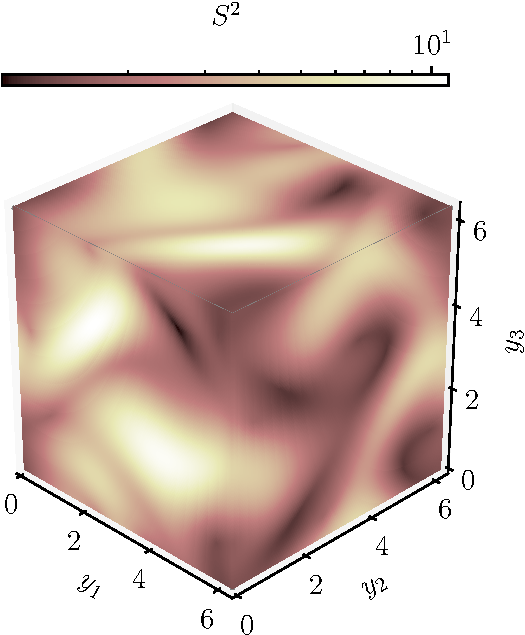
\includegraphics[width=\textwidth]{chp04_paper_numerics/figures/gabc/S2_box_1.0_cropped}
		% 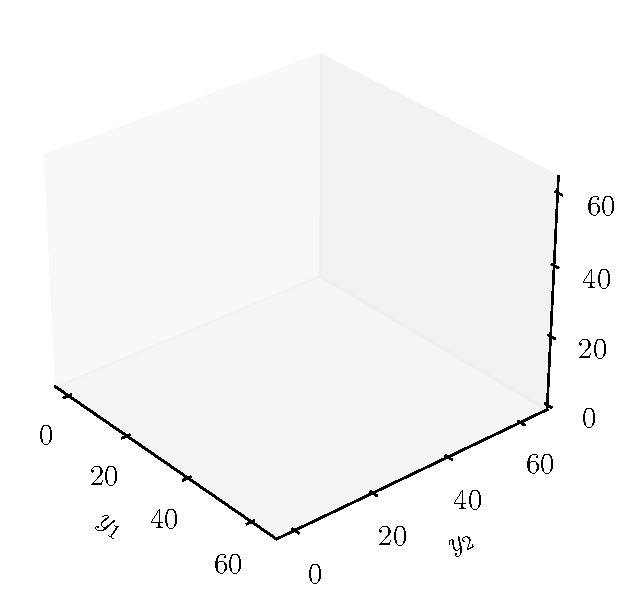
\includegraphics[width=0.49\textwidth]{chp04_paper_numerics/figures/gabc/robust_box_1}
		\caption{\(t = 1\)}
		\label{fig:gabc_S2_1}
	\end{subfigure}
	\begin{subfigure}[t]{0.49\textwidth}
		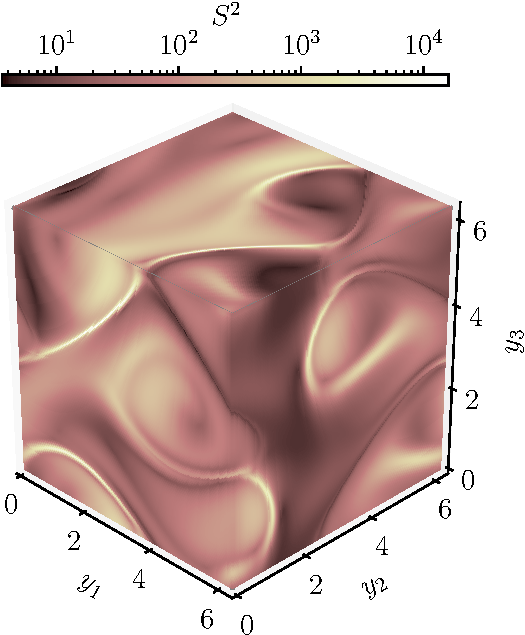
\includegraphics[width=\textwidth]{chp04_paper_numerics/figures/gabc/S2_box_3.0_cropped}
		% 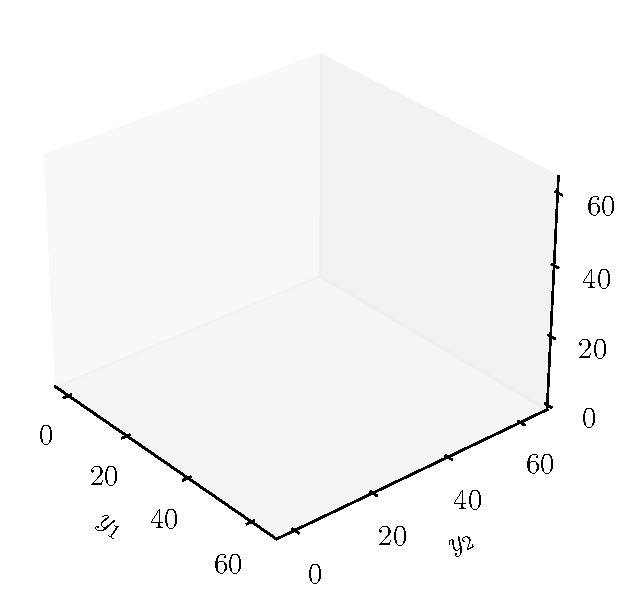
\includegraphics[width=0.49\textwidth]{chp04_paper_numerics/figures/gabc/robust_box_1}
		\caption{\(t = 3\)}
		\label{fig:gabc_S2_3}
	\end{subfigure}
	\caption{The stochastic sensitivity field for the GABC flow \cref{eqn:gabc} with identity diffusion, over the time interval \([0,t]\).}%, and robust sets (right) extracted with a threshold of \(R = 0.8\).}
	\label{fig:gabc_S2}
\end{figure}

To introduce 3-dimensional noise to the system, we set \(\sigma \equiv I\), the \(3 \times 3\) identity matrix, and compute stochastic sensitivity for a \(200\times 200\) grid of initial conditions on each face of the cube \([0,2\pi] \times [0,2\pi] \times [0,2\pi]\).
The spatial periodicity and symmetry of the dynamics means that these three faces are sufficient to describe the entire structure of the field within the region \citep{DombreEtAl_1986_ChaoticStreamlinesABC}.
As with the two-dimensional example, for each initial condition we compute the \(3 \times 3\) covariance matrix using the Mazzoni method.
The stochastic sensitivity value is then computed by taking the operator norm of this covariance matrix.
\Cref{fig:gabc_S2} plots the stochastic sensitivity on the three faces of the cube, at two different times.
At \(t = 1\) (\Cref{fig:gabc_S2_1}), the vortex structures are highlighted by the stochastic sensitivity field, in that these regions have a higher uncertainty due to the ??
\td{Interpret - looks like the vortex structures are hilighted by the field?}
When \(t = 3\) (\Cref{fig:gabc_S2_3}), the flow is domainated by chaotic mixing, but we nonetheless see structures highlighted by the stochastic sensitivity...!!!
In fact, these narrow ridge-like structures correspond to the unstable manifolds within the flow \citep{DombreEtAl_1986_ChaoticStreamlinesABC}: the repelling nature of these regions results in a `larger' stochasticity.

\chapter{A Gaussian mixture model}\label{ch:gmm}
In \Cref{ch:linear_theory}, we described and justified a framework for computing approximations to the solutions of non-linear SDEs via linearisations about solutions to the corresponding deterministic system.
A key advantage of this approximation is efficiency of computation; rather than having to generate a large number of realisations of the SDE solution to understand, either qualitatively or for the purposes of inference and estimation, the probability distribution of the solution, we can solve a smaller system of differential equations to obtain the first two moments.
When the initial condition is fixed or Gaussian, the resulting linearisation solution is a Gaussian process, providing an approximation characterised \emph{entirely} by these two moments.
A Gaussian approximation has further advantages, leading to its use across many different applications \citep{KaszasHaller_2020_UniversalUpperEstimate,ArchambeauEtAl_2007_GaussianProcessApproximations,Jazwinski_2014_StochasticProcessesFiltering,SarkkaSolin_2019_AppliedStochasticDifferential,Sanz-AlonsoStuart_2017_GaussianApproximationsSmall}.
For example, even in inference requiring Monte-Carlo simulations, a Gaussian distribution with a specified mean and covariance is faster to sample from than generating numerical solutions of the nonlinear SDE.

However, this approximation is only `reasonable' in the limit of small initial and ongoing uncertainty, which we quantified exactly with the bound in \Cref{thm:main}, and demonstrated heuristically with examples in \Cref{fig:sine_hists,fig:1d_mult_hists,fig:y_hists}.
In practice, the scale of the noise is an inherent part of a model and there is no guarantee that it is sufficiently small for Gaussian approximations to be reasonable.
When the noise scale is larger, we see non-Gaussianity emerge---the numerical solutions in \Cref{fig:sine_hists,fig:1d_mult_hists,fig:y_hists} exhibit skewness, bi-modality, and other departures from Gaussianity.
Although the Gaussian approximation can still provide qualitative insight into the behaviour of these solutions (see stochastic sensitivity, for instance), to produce a reasonable approximation we need a method that can capture these departures from Gaussianity.

\begin{figure}
	\centering
	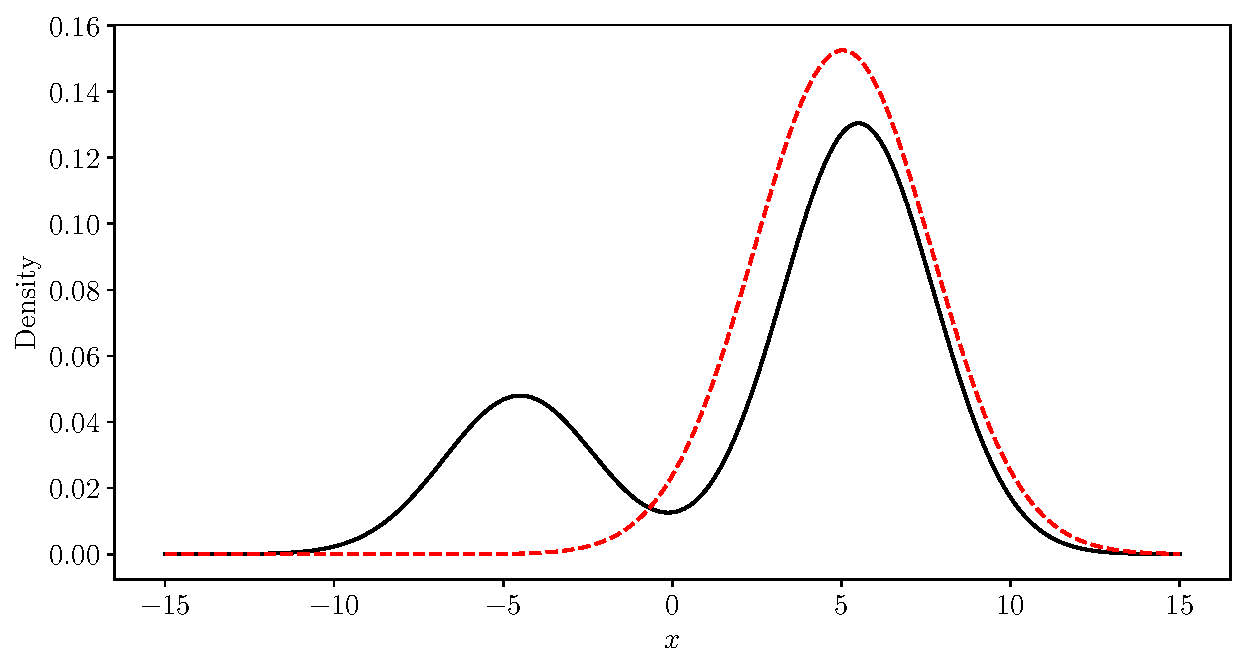
\includegraphics[width=0.9\textwidth]{chp05_gmm/figures/bene_final_gauss_5.0.pdf}
	\caption{The probability density function \cref{eqn:bene_sde_pdf} of the solution \(x_5\) (in black) to Ben\^e's SDE \cref{eqn:bene_sde}, with fixed initial condition \(x_0 = 1/2\).
		The density function of the Gaussian solution to the corresponding linearisation is overlaid in dashed red.}
	\label{fig:bene_gauss}
\end{figure}

To further illustrate this point, we consider another example of a 1-dimensional stochastic differential equation.
Ben\^e's SDE \citep{SarkkaSolin_2019_AppliedStochasticDifferential} is
\begin{equation}
	\dif x_t = \tanh\!\left(x_t\right)\dif t + \dif W_t.
	\label{eqn:bene_sde}
\end{equation}
In this example we are implicitly taking \(\epsilon = 1\), which is a larger noise scale than we typically expect to apply our results to.
However, this example is purely demonstrative to highlight a limitation of Gaussian approximations and show the potential of the algorithm we are about to propose; later examples will involve a smaller noise scale.
The deterministic system corresponding to \cref{eqn:bene_sde} is
\begin{equation}
	\dod{F_0^t\!\left(x_0\right)}{t} = \tanh\!\left(F_0^t\!\left(x_0\right)\right),
	\label{eqn:bene_ode}
\end{equation}
which includes an unstable fixed point at \(0\).
We consider the solution to \cref{eqn:bene_sde} subject to the fixed initial condition \(x_0 = 1/2\) and at time \(t = 5\).
The probability density function of the weak solution to \cref{eqn:bene_sde} can be derived using an appropriate change of measure with Girsanov's theorem (see Section 7.3 of \citet{SarkkaSolin_2019_AppliedStochasticDifferential}.
The probability density function for the solution \(x_t\) at time \(t = 5\) is given by
\begin{equation}\label{eqn:bene_sde_pdf}
	p(x) = \frac{1}{\sqrt{10\pi}}\frac{\cosh\left(x\right)}{\cosh\!\left(\frac12\right)}\exp\left[-\frac{5}{2} - \frac{1}{10}\left(x - \frac12\right)^2\right],
\end{equation}
and is plotted in black in \Cref{fig:bene_gauss}.
The density is not symmetric with two distinct modes that result from the unstable fixed point of \cref{eqn:bene_ode} at \(x = 0\).
Many stochastic trajectories are driven away from zero, resulting in the predominant mode centred at \(x = 5.5\).
However, when the stochastic perturbations force a trajectory through the fixed point and into negative values, they are pushed further in the negative direction, leading to the second mode at \(x = -4.5\).
Nonetheless, we can linearise \cref{eqn:bene_sde} about the deterministic trajectory \(F_0^t\!\left(1/2\right)\) solving \cref{eqn:bene_ode} to obtain a Gaussian approximation, which we also plot the density of in dashed red in \Cref{fig:bene_gauss}.
The Gaussian approximation cannot capture the bimodality of the true solution, and so only a single mode is captured.
This is a significant limitation of using a single linearisation approximation, which cannot possibly capture any multimodality.
% However, to compensate for the additional negative mode, the mean of the Gaussian approximation is less than that of the positive mode, and the variance is larger.\lb{Again, need to be more precise here. Have a look at the conditional probabilities and compare - the deterministic trajectory would have no idea about the fixed point. Otherwise could omit this sentence - keep it simple, the main point is the bimodality}


% \newcommand{\plotbenepdf}[2]{
% 	\begin{tikzpicture}\begin{axis}[
% 				ymin=0.0,
% 				xmin=-10.0,
% 				xmax=10.0,
% 				axis lines=center,
% 				axis on top=true,
% 				domain=-10:10,
% 				ylabel=$p$,
% 				xlabel=$x$,
% 				ytick=\empty,
% 				yticklabels={},
% 			]
% 			\addplot [mark=none,draw=black,thick,samples=500] {cosh(\x)*exp(-#2/2-1/(2 * #2)*(\x-#1)^2)/((2 * pi * #2)^(1/2) * cosh(#1))};
% 		\end{axis}
% 	\end{tikzpicture}
% }

% \begin{figure}
% 	\begin{center}
% 		\begin{subfigure}{0.49\textwidth}
% 			\plotbenepdf{1/2}{1}
% 			\caption{\(t = 1\)}
% 			\label{fig:bene_1}
% 		\end{subfigure}
% 		\begin{subfigure}{0.49\textwidth}
% 			\plotbenepdf{1/2}{2.5}
% 			\caption{\(t = 2.5\)}
% 			\label{fig:bene_2.5}
% 		\end{subfigure}
% 		\begin{subfigure}{0.49\textwidth}
% 			\plotbenepdf{1/2}{5}
% 			\caption{\(t = 5\)}
% 			\label{fig:bene_5}
% 		\end{subfigure}
% 		\begin{subfigure}{0.49\textwidth}
% 			\plotbenepdf{1/2}{7.5}
% 			\caption{\(t = 7.5\)}
% 			\label{fig:bene_7.5}
% 		\end{subfigure}
% 	\end{center}
% 	\caption{The probability density function \cref{eqn:bene_sde_pdf} for the time-marginal solution of Ben\^e's SDE \cref{eqn:bene_sde}, for the initial condition \(x_0 = 1/2\) at various times.
% 		The density function consists of two distinct modes that move further apart as \(t\) increases.}
% 	\label{fig:bene_pdf}
% \end{figure}



We seek a scheme that can capture departures from Gaussianity in the SDE solution, while still taking advantage of the efficient computation of the corresponding deterministic system and the linearisation approximation.
An alternative perspective of the linearisation solution is that it captures the behaviour of stochastic fluctuations close to a deterministic trajectory, in a similar sense to how a Taylor polynomial captures local behaviour of a nonlinear function.
By `piecing' together several of these approximations together we can capture the stochastic behaviour in different regions of the state space.
A Gaussian mixture model (GMM) provides a framework for combining multiple Gaussian densities into a single distribution, and is therefore the obvious choice for constructing non-Gaussian densities out of our Gaussian approximations.
In this chapter, we outline an algorithm that uses \emph{multiple} Gaussian approximations resulting from the linearised SDE in a mixture model to provide a non-Gaussian approximation to the nonlinear SDE solution.
The algorithm itself is provided in \Cref{sec:gmm_alg}.

% Helper functions for TikZ pic
\newcommand{\TikZGauss}[3]{1 / sqrt(2 * pi * #3) * exp(-(#1 - #2) * (#1 - #2) / #3)} % Args: variable, mean, variance
\newcommand{\TikZMixtureTwo}[8]{% Args: width, comp1_mean, comp1_var, comp2_mean, comp2_var, comp1_weight, comp2_weight, vertical scaling
	\begin{tikzpicture}
		% Two components
		\draw[domain=0:#1, smooth, variable=\x, dashed] plot ({\x}, {#8 * \TikZGauss{\x}{#2}{#3}});
		\draw[domain=0:#1, smooth, variable=\x, dashed] plot ({\x}, {#8 * \TikZGauss{\x}{#4}{#5}});
		% Mixture model
		\draw[domain=0:#1, smooth, variable=\x, very thick] plot ({\x}, {#8 * #6 * \TikZGauss{\x}{#2}{#3} + #8 * #7 * \TikZGauss{\x}{#4}{#5}});
		\draw[thick] (0,0)--(#1,0); % node[right]{\(x\)};
	\end{tikzpicture}
}

\begin{figure}
	\centering
	\begin{subfigure}{0.49\textwidth}
		\TikZMixtureTwo{7}{2}{1}{3}{2}{0.5}{0.5}{3}
		\caption{Skewness}
	\end{subfigure}
	\begin{subfigure}{0.49\textwidth}
		\begin{tikzpicture}
			\TikZMixtureTwo{7}{2}{1}{4.5}{0.5}{0.5}{0.5}{3}
		\end{tikzpicture}
		\caption{Bimodality}
	\end{subfigure}
	\caption{The probability density functions of two Gaussian mixture models in 1-dimension both using two equally weighted components.
		The individual components (dashed) are combined to produce the non-Gaussian mixture density (solid) which can exhibit skewness and bimodality.}
	\label{fig:mixture_model}
\end{figure}

In general, a Gaussian mixture model with \(K\) components is a probability density function of the form
\[
	p(z) = \sum_{k=1}^{K}{\omega_i \Gauss{z;\, \mu^{(i)}, \Sigma^{(i)}}},
\]
which consists of \(K\) Gaussian components \(\Gauss{\mu^{(i)}, \Sigma^{(i)}}\) with respective weights \(\omega_1, \dotsc, \omega_K \geq 0\) satisfying \(\sum_{k=1}^{K}\omega_k = 1\).
With sufficient components, a Gaussian mixture model can recreate any probability distribution in \(\R^n\) while having many of the properties that make Gaussian distributions appealing in practice \citep{McLachlanEtAl_2019_FiniteMixtureModels}.
\Cref{fig:mixture_model} shows three examples of Gaussian mixture models in 1-dimension, where departures from Gaussianity such as multimodality and skewness can be captured with an appropriate combination of components.


% \begin{figure}
% 	\begin{center}
% 		\begin{tikzpicture}
% 			\draw[scale=2, domain=-3:4, smooth, variable=\x, dashed] plot ({\x}, {exp(-(\x + 0.5) * (\x + 0.5))});
% 			\draw[scale=2, domain=-3:4, smooth, variable=\x, dashed] plot ({\x}, {1 / (sqrt(2 * pi * 0.8))*exp(-(\x - 1.5) * (\x - 1.5) / 0.8)});
% 			\draw[scale=2, domain=-3:4, smooth, variable=\x, thick] plot ({\x}, {0.5 * exp(-(\x + 0.5) * (\x + 0.5)) + 0.5 * 1 / (sqrt(2 * pi * 0.8))*exp(-(\x - 1.5) * (\x - 1.5) / 0.8)});
% 			\draw[->,thick] (-6,0)--(8,0) node[right]{\(x\)};
% 		\end{tikzpicture}
% 		\caption{An example of the probability density function of a Gaussian mixture model with two weighted components.
% 		The two individual components (dashed) are combined to produce the non-Gaussian mixture density (solid).}
% 		\label{fig:mixture_model}
% 	\end{center}
% \end{figure}


% We have a ``local'' approximation for the SDE \cref{eqn:sde_no_eps}, in that solutions to the linearised equation capture the solution behaviour nearby a given deterministic trajectory.
% In practice, the solution to stochastic differential equations are non-Gaussian.
% A key observation of \Cref{sec:theory_gauss} is that the solution to the linearised SDE is Gaussian when the initial condition is Gaussian.
% Through a mixture model, we can capture this non-Gaussianity (leading to a better approximation) while still taking advantage of the computationally efficiency of the Gaussian approximation.

\section{Mazzoni's method}\label{sec:mazzoni}
\td{May need to reconsider ordering of sections here - this could go after describing the mixture model.}
Prior to outlining our mixture model algorithm, we will first detail a computationally efficient method for computing the Gaussian solution to a linearised SDE.
We are interested in approximating the solution at a time \(t\) to the nonlinear stochastic differential equation
\begin{equation}
	\dif y_t = u\!\left(y_t, t\right)\dif t + \epsilon\sigma\!\left(y_t, t\right)\dif W_t,
	\label{eqn:sde_y_gmm}
\end{equation}
subject to some random initial condition \(y_s = x\), by using solutions of the corresponding deterministic system
\begin{equation}
	\dod{F_s^t\!\left(x_0\right)}{t} = u\!\left(F_s^t\!\left(x\right), t\right), \quad F_s^s\!\left(x\right) = x.
	\label{eqn:det_ode_gmm}
\end{equation}
The behaviour of the solution \cref{eqn:sde_y_gmm} over the time interval \((s,t)\) for small \(\epsilon\) can be approximated by the linearised SDE
\begin{equation}
	\dif l_t = \left(u\!\left(F_s^t\!\left(x\right), t\right) + \nabla u\!\left(F_s^t\!\left(x\right), t\right)\left[l_t - F_s^t\!\left(x\right)\right]\right)\dif t + \epsilon\sigma\!\left(F_s^t\!\left(x\right), t\right)\dif W_t,
	\label{eqn:sde_linear_gmm}
\end{equation}
subject to the initial condition \(l_s = x\).
The theory in \Cref{ch:linear_theory} considered the evolution of \cref{eqn:sde_y_gmm} over a time interval \((0,t)\) and subject to some initial condition at time \(0\).
However, by using a simple time shift our theory can be applied to any finite time interval \((s,t)\), where the solution is specified at time \(s\) instead of \(0\), without loss of generality.
Note that we have now also dropped the dependence of \(\epsilon\) in the notation \(y_t\) and \(l_t\), as \(\epsilon\) is now treated as a fixed value specified as part of the model.
Suppose that the initial condition \(x\) follows a Gaussian distribution with mean \(x_0\) and a specified covariance matrix \(\Sigma_s\).
If the initial condition is fixed as \(x_s\), then we set \(\Sigma_s = O\), the \(n \times n\) zero matrix, so that the initial distribution is a Dirac delta.
We will focus our attention on this case for the remainder of this thesis, having already provided a general framework in \Cref{ch:linear_theory} for other initial conditions.
By taking the mean \(x_s\) as the initial condition to \cref{eqn:det_ode_gmm}, we ensure that the initial uncertainty (measured by the \(L_r\)-norm as in \Cref{ch:linear_theory}) scales with the trace of \(\Sigma_s\).
The solution to \cref{eqn:sde_linear_gmm} is then a Gaussian process characterised by the mean \(F_s^t\!\left(x_0\right)\) and covariance matrix \(\var{l_t}\), for which explicit expressions for are given in \Cref{cor:limit_moments}.
For notational brevity, set \(w_t \equiv F_s^t\!\left(x_s\right)\) and \(\Pi_t \equiv \var{l_t}\).
When the Jacobian \(\nabla u\) of the vector field \(u\) is available, or can approximated appropriately, the moments of the Gaussian solution can be obtained by the system of ordinary differential equations
\begin{subequations}\label{eqn:gauss_de}
	\begin{align}
		\dod{w_t}{t}   & = u\!\left(w_t, t\right), \quad w_s = x_0 \label{eqn:gauss_mean_de}                                                                                                           \\
		\dod{\Pi_t}{t} & = \begin{multlined}[t]
			                   \nabla u\!\left(w_t, t\right) \Pi_t + \Pi_t\left[\nabla u\left(w_t, t\right)\right]^{\T} + \sigma\left(w_t, t \right)\sigma\left(w_t, t\right)^{\T}, \quad \Pi_s = \Sigma_s.
		                   \end{multlined}
		\label{eqn:gauss_cov_de}
	\end{align}
\end{subequations}
In practice, \cref{eqn:gauss_de} must be solved numerically, but can be more computationally efficient than the alternative of generating many realisations of \cref{eqn:sde_y_gmm}.
Thus, we can efficiently compute a Gaussian approximation \(\Gauss{w_t, \Sigma_t}\) to the solution to the nonlinear SDE \cref{eqn:sde_y_gmm} at time \(t\) by solving \cref{eqn:gauss_de} only.

An important consideration  when solving \cref{eqn:gauss_de} numerically is that \(\Pi_t\) represents a covariance matrix and must remain symmetric and positive semi-definite.
However, many standard numerical ODE schemes do not take this into account, so a specialised scheme is required.
Similar equations of the form \cref{eqn:gauss_de} (although often without explicit dependence on both time and the state in the \(\sigma\) term) are solved numerically in other applications, notably when implementing the extended Kalman filter \citep{Jazwinski_2014_StochasticProcessesFiltering, KulikovaKulikov_2014_AdaptiveODESolvers}.
\citet{KulikovaKulikov_2014_AdaptiveODESolvers} identify that that the two most significant sources of numerical error when solving \cref{eqn:gauss_de} are a) the estimate of the covariance matrix \(\Sigma_s^t\) violating the requirement of positive semi-definiteness, and b) local error propagation in the state equation.
Moreover, a computationally efficient algorithm is critical to ensure that our approximate methods have an advantage over bulk Monte-Carlo simulation.

\citet{Mazzoni_2008_ComputationalAspectsContinuous} proposes an efficient hybrid method for solving \cref{eqn:gauss_de} which addresses both difficulties a) and b) and takes advantage of the availability of \(\nabla u\).
This method, which we shall term the Mazzoni method, combines a Taylor-Heun approximation for \cref{eqn:gauss_mean_de} and a Gauss-Legendre step for \cref{eqn:gauss_cov_de}.
With a step size of \(\delta t\), integration for both the state variable and the covariance matrix are convergent with order \(\mathcal{O}\!\left(\delta t^2\right)\).
Moreover, \citet{Mazzoni_2008_ComputationalAspectsContinuous} shows through numerical simulations that the algorithm is computationally efficient when compared to alternatives with moderate precision.
We therefore employ the Mazzoni method for all subsequent computations of the linearisation solution.

The Mazzoni algorithm is summarised in the following.
Further details on the derivation of these equations is available in the original article \citep{Mazzoni_2008_ComputationalAspectsContinuous}.
The Taylor-Heun formula for the update of the state over the interval \([t, t + \delta t]\) is
\begin{subequations}\label{eqn:mazzoni_update}
	\begin{equation}
		w_{t + \delta t} \approx w_t + \left(I - \frac{\delta t}{2}\nabla u\left(w_t, t\right)\right)^{-1}.
		\label{eqn:mazzoni_state_update}
	\end{equation}
	The Gauss-Legendre update of the covariance matrix is
	\begin{equation}
		\Pi_{t + \delta t} \approx M_\tau \Pi_t M_\tau^{\T} + \delta t K_\tau \sigma\left(w_\tau,\, t + \frac{\delta t}{2}\right)\sigma\left(w_\tau,\, t + \frac{\delta t}{2}\right)^{\T} K_\tau^{\T},
		\label{eqn:mazzoni_cov_update}
	\end{equation}
	where
	\begin{align}
		w_\tau & = \frac12\left(w_t + w_{t + \delta t} - \frac{\delta t^2}{4}\nabla u\left(w_t, \, t\right) u\left(w_t, \, t\right)\right) \label{eqn:mazzoni_cov_terms1} \\
		K_\tau & = \left[I - \frac{\delta t}{2}\nabla u\left(w_\tau,\, t + \frac{\delta t}{2}\right)\right]^{-1}                                                          \\
		M_\tau & = K_\tau \left[I + \frac{\delta t}{2}\nabla u\left(w_\tau,\, t + \frac{\delta t}{2}\right)\right] \label{eqn:mazzoni_cov_terms3}.
	\end{align}
	The vector \(w_\tau\) serves as an interpolation between \(w_t\) and \(w_{t + \delta t}\) for the state at time \(t + \delta t / 2\), which is used to provide a more accurate approximation of the covariance matrix.
	\citet{Mazzoni_2008_ComputationalAspectsContinuous} also provides the option of an adaptive time step to fix the numerical precision while ensuring a computationally efficient algorithm.
	The step size is adjusted by monitoring the error in the estimation of the state variable, aiming to maintain a specified tolerance level \(\gamma > 0\).
	Given the error vector \(\mathcal{E}\) for each component of the state approximation, the maximum total-relative error is
	\begin{equation}\label{eqn:mazzoni_e}
		\hat{\gamma} = \max_{i = 1,\dots,n}\frac{\abs{\mathcal{E}^{(i)}}}{\abs{w_{t + \delta t}^{(i)}} + 1}
	\end{equation}
	where \(\mathcal{E}^{(i)}\) and \(w_{t + \delta t}^{(i)}\) denote the respective \(i\)th elements of \(\mathcal{E}\) and \(w_{t + \delta t}\).
	The resulting adjustment factor for the time step is
	\begin{equation}\label{eqn:mazzoni_step}
		\delta t_{\mathrm{new}} = \beta \delta t \sqrt{\frac{\gamma}{\hat{\gamma}}}.
	\end{equation}
	The factor \(\beta\) is a control parameter inserted to avoid frequent recalculations of the step size, and is specified prior.
	\citet{Mazzoni_2008_ComputationalAspectsContinuous} suggests setting \(\beta = 0.8\).
	By again taking advantage of the availability of the Jacobian \(\nabla u\), the error vector is approximated as
	\begin{equation}\label{eqn:mazzoni_err}
		\mathcal{E} \approx \frac{\delta t^2}{2}\left[\frac{1}{3\delta t}\left(\nabla u\!\left(w_{t + \delta t}, t + \delta t\right) - \nabla u\!\left(w_t, t\right)\right) - \frac{1}{6}\nabla u\!\left(w_t, t\right)^2\right] u\!\left(w_t, t\right).
	\end{equation}
\end{subequations}
The set of equations \cref{eqn:mazzoni_update} describe the Mazzoni algorithm, and in \Cref{fig:mazzoni_alg} we summarise the full algorithm with an adaptive step size.

\begin{figure}
	\begin{center}
		\usetikzlibrary{shapes.geometric, arrows, positioning}

		\begin{tikzpicture}[node distance=70pt]
			\tikzstyle{arrow} = [->,>=stealth]

			\node (s) [rectangle, rounded corners, draw=black, align=center] {\textbf{Start} \\ Given \(s, T, x_s, \Sigma_s\) \\ Choose \(\delta t_{\mathrm{min}}, \beta, \gamma\)};

			\node (a) [rectangle, below of=s, draw=black, align=center, yshift=-10pt] {Set \(t_0 = s\) \\ Set \(w_{t_0} = x_s\) \\ Set \(\Pi_{t_0} = \Sigma_s\) Set \(\delta t = \delta t_{\mathrm{min}}\) \\ Set \(k = 0\)};
			\node (b) [rectangle, below of=a, draw=black, align=center, yshift=-20pt] {Set \(t_{k+1} = t_k + \delta t\) \\ Compute \(w_{t_{k+1}}\) with \cref{eqn:mazzoni_state_update} \\
				Compute \(e\) with \cref{eqn:mazzoni_e} \\ Set \(\delta t_{\mathrm{new}} = \max\left\{\delta t_{\mathrm{min}}, \beta \delta t \sqrt{\frac{\gamma}{\hat{\gamma}}}\right\}\)};

			\node (d) [diamond, below of=b, draw=black, align=center, yshift=-40pt] {\(\hat{\gamma} \leq \gamma\) or \\ \(\delta t \leq \delta t_{\mathrm{min}}\)?};
			\node (c) [rectangle, left of=d, draw=black, align=center, xshift=-75pt] {Set \(\delta_t = \delta_{\mathrm{new}}\)};

			\node (e) [rectangle, below of=d, draw=black, align=center, yshift=-20pt] {Compute \(\Pi_{t_{k+1}}\) with \crefrange{eqn:mazzoni_cov_terms1}{eqn:mazzoni_cov_terms3} \\ Set \(k = k + 1\)};

			\node (f) [diamond, below of=e, draw=black, align=center] {\(t_k = T\)?};

			\node (g) [rectangle, rounded corners, left of=f, draw=black, align = center, xshift = -30pt] {\textbf{Stop}};
			\node (h) [rectangle, right of=f, draw=black, align = center, xshift = 75pt] {\(\delta t = \min\left\{\delta t_{\mathrm{new}}, T - t_k\right\}\)};

			\draw [arrow] (s) -- (a);

			\draw [arrow] (a) -- (b);
			\draw [arrow] (b) -- (d);

			\draw [arrow] (d) -- node[anchor=south] {no} (c);
			\draw [arrow] (d) -- node[anchor=east] {yes} (e);

			\draw [arrow] (c) |- (b);

			\draw [arrow] (e) -- (f);

			\draw [arrow] (f) -- node[anchor=south] {yes} (g);
			\draw [arrow] (f) -- node[anchor=south] {no} (h);

			\draw [arrow] (h) |- (b);
		\end{tikzpicture}
		\caption{A flowchart of the Mazzoni algorithm with adaptive time stepping.
			Recreated from Figure 2 of \citet{Mazzoni_2008_ComputationalAspectsContinuous}.}
		\label{fig:mazzoni_alg}
	\end{center}
\end{figure}





\section{The GMM algorithm}\label{sec:gmm_alg}
Let us now return to the original aim of this chapter: to approximate the SDE solution with a Gaussian mixture model while taking advantage of the computationally efficiency of the Gaussian linearisation approximation.
Given a Gaussian component at a time \(s\), we can `propagate` the component forward to a later time \(t\) by solving \Cref{eqn:gauss_de} initialised with the component mean and covariance matrix.
That is, we are updating the mean and covariance of the Gaussian component by approximating the solution to the original SDE \cref{eqn:sde_y_gmm} over \((s,t)\) with a linearisation about the deterministic trajectory initialised from the component mean.
Given a mixture model with multiple Gaussian components, we can propagate each component separately to update the full model through time in a computationally efficient manner.

Our proposed method is ad-hoc and based on a simple intuition: the Gaussian solution provides a reasonable approximation for the local behaviour of the true SDE solution over a short timeframe, but once this is no longer the case, we can capture departures from Gaussianity by introducing more components into the mixture model.
We expect heuristically that as the number of components increase, the full mixture model should provide a closer approximation of the SDE solution density, provided that the components are appropriately placed.
However, our goal is to provide a numerically efficient algorithm, so we wish to minimise the number of components and use the Gaussian approximation where ever possible.
We therefore propose propagating Gaussian components forward through the linearisation model until are no longer reasonable approximations of the local solution behaviour.
Then, we replace violating component with several smaller judiciously chosen components and propagate each new component individually.
We term this the \emph{splitting} step, where a Gaussian component is split into several smaller ones.
The new components should be chosen in such a way as to preserve the original component, which can be achieved as follows.
Let \(\Xi\) follow a Gaussian mixture density with \(N\) components, with respective weights \(w^{(1)}, \dotsc, w^{(N)}\), means \(\mu^{(1)},\dotsc,\mu^{(N)}\), and covariance matrices \(\Sigma^{(1)},\dotsc,\Sigma^{(N)}\).
The variance of the mixture model is then
\begin{align*}
	\var{\Xi} & = \sum_{i=1}^{N}{w^{(i)}\Sigma^{(i)}} + \sum_{i=1}^{N}{w^{(i)}\left(\mu^{(i)} - \bar{\mu}\right)\left(\mu^{(i)} - \bar{\mu}\right)^{\T}} \\
	          & = \text{Mean of covariances} + \text{Covariance of means},
\end{align*}
where \(\bar{\mu} = \sum_{i=1}^{N}{w^{(i)}\mu^{(i)}}\).
This decomposition suggests, at least heuristically, that we can include additional uncertainty (in the form of contributions to the overall variance) within the component means themselves.
By replacing a single component with points, we can ``preserve'' the mean and covariance of the component while introducing additional components that can closer match the non-Gaussian distribution we are seeking to approximate.
This leads to the following condition on how a component is split: the splitting points should be chosen so that
\begin{equation}
	\frac{1}{K}\sum_{i=1}^K{x^{(k)}} = x, \quad \frac{1}{K}\sum_{i=1}^{K}{\left(x^{(k)} - x\right)\!\left(x^{(k)} - x\right)^{\T}} = \Sigma_0.
	\label{eqn:cov_split_points}
\end{equation}
This ensures that the mean and covariance of the original Gaussian is preserved within the (sample) mean and covariance of the new points themselves.
Note that at least \(K = n + 1\) points are necessary for \cref{eqn:cov_split_points} to be satisfied.
The selection of splitting points are similar to the notion of `sigma points`, employed in the unscented transform to encode an initial mean and covariance \citep{Uhlmann_1995_DynamicMapBuilding,JulierEtAl_2000_NewMethodNonlinear}.
Any such sigma points satisfy \cref{eqn:cov_split_points}---Table I by \citet{MenegazEtAl_2015_SystematizationUnscentedKalman} provides a list of sigma points used across other literature (and reviewed in the context of Kalman filtering)---and therefore can be used in our algorithm.
% However, we note a key difference between our proposed algorithm and the unscented transform; the unscented transform provides an \emph{exact} estimate of.
The canonical set of sigma points originally proposed by \citet{Uhlmann_1995_DynamicMapBuilding}, which we use to apply the GMM algorithm in \Cref{ch:appls}, are
\begin{subequations}\label{eqn:uhlman_sigma}
	\begin{align}
		x^{(0)}     & = x,                                                                                              \\
		x^{(i)}     & = x + \sqrt{n + \frac12}\left[\sqrt{\Sigma}\right]_{\cdot i}, \\
		x^{(n + i)} & = x - \sqrt{n + \frac12}\left[\sqrt{\Sigma}\right]_{\cdot i},
	\end{align}
\end{subequations}
for \(i = 1,\dotsc, n\), where \(\sqrt{\Sigma}\) denotes the symmetric square root of \(\Sigma\), and \(\left[\sqrt{\Sigma}\right]_{\cdot i}\) denotes the \(i\)th column of \(\sqrt{\Sigma}\).
However, we do not enforce a particular approach for selecting these points and leave this to be investigated further as future work.

The mixture model algorithm is then as follows:
\begin{enumerate}
	\item Initialise a Gaussian mixture model with \(N\) components, setting \(t^{(1)} = 0\), \(x^{(1)},\dotsc, x^{(N)}\) to be the component means, \(\Sigma^{(1)}, \dotsc, \Sigma^{(N)}\) to be the component covariance matrices, and \(w^{(1)}, \dotsc, w^{(N)}\) to be the component weights.

	\item While \(t^{(i)} < T\) for any \(i = 1,\dotsc, N\), iterate the following;

	      \begin{enumerate}
		      \item Set \(j\) to be any \(i\) for which \(t^{(i)} < T\).

		      \item Update \(x^{(j)}\) and \(\Sigma^{(j)}\) by solving the joint system \cref{eqn:gauss_de} with initial state \(x^{(j)}\) and covariance \(\Sigma^{(j)}\), terminating when a split condition is met or the final time \(T\) is reached.
		            Denote the time at which this solution terminates as \(t^{(i)}\).

		      \item If \(t = T\), then complete this branch of the algorithm and continue along another branch, if any are still incomplete.

		      \item Otherwise, if \(t < T\), construct \(2n\) points \(x^{(N + 1)},\dotsc,x^{(N + 2n)}\) that preserve the propagated mean and covariance (i.e. satisfying \cref{eqn:cov_split_points}), setting
		            \[
			            \Sigma^{(N + k)} = \Sigma^{(1)}, \quad \text{and} \quad w^{(N + k)} = \frac{w^{(1)}}{2n} \quad \text{for each } k = 1,\dotsc,K
		            \]
		            and \(\Sigma^{(1)} = \Sigma^{(1)}\), \(w^{(1)} = w^{(1)} / 2n\), and \(N = N + K\).
	      \end{enumerate}

	\item Construct the mixture model with density function
	      \[
		      G\left(x\right) = \frac{1}{\sum_{l=1}^{N}w^{(l)}}\sum_{i=1}^{N}{w^{(i)}\Gauss{x; \, x^{(i)}, \Sigma^{(i)}}}.
	      \]

\end{enumerate}
\td{I probably should comment on the weighting. When a component is split, the new components are weighted so the sum of weights of the new points equals that of the original.}
\Cref{fig:gmm_steps} provides a pictorial representation of the propagation and splitting of a single component in the mixture model.
We have presented a general framework, with several choices for specific implementations that are left unfulfilled or could be improved with further investigation.

There are several options for initialising the mixture model, depending on the initial condition at time \(0\).
For a fixed initial condition \(x_0\), we can take the degenerate mixture model with a single component and zero variance, i.e.
\[
	N = 1, \quad x^{(1)} = x_0, \quad \Sigma^{(1)} = O, \quad w^{(1)} = 1.
\]
If the initial condition is Gaussian, this can be used as a single component mixture model and propagated forward with \cref{eqn:gauss_de} by including the initial covariance matrix as the initial condition for the covariance equation.
\td{comment on non-Gaussian initial conditions..? The framework is flexible and can work with any Gaussian mixture model initialisation, so just need to represent an arbitrary initial density with a mixture model.}

\begin{figure}
	\captionsetup{singlelinecheck=off}
	\begin{center}
		\begin{tikzpicture}
			\draw (-1,4) node {1)};
			% STEP 0: INITIAL
			% Initial position
			\fill[black] (1,1.5) circle[radius=1pt] node[anchor = east] {\(x\)};

			% Initial covariance
			\draw[dashed, rotate around = {58: (1, 1.5)}, blue] (1,1.5) ellipse (14pt and 22pt);
			\node[blue] at ($(1,1.5)+(90:14pt and 22pt)$) {\(\Sigma_0\)};

			% STEP 1: PROPAGATE
			\draw (6,4) node {2)};
			% Trajectory
			\draw (7,1.5) .. controls (9,3.5) and (11,-1.5) .. (13,1.5);

			% Initial position
			\fill[black] (7,1.5) circle[radius=1pt] node[anchor = east] {\(x\)};

			% Initial covariance
			\draw[dashed, rotate around = {58: (7, 1.5)}, gray] (7,1.5) ellipse (14pt and 22pt);

			% Mapped position
			\fill[black] (13,1.5) circle[radius=1pt] node[anchor = south] {\(F_0^t\!\left(x\right)\)};

			% Covariance ellipse
			\draw[dashed, rotate around = {30: (13,1.5)}, red] (13,1.5) ellipse (30pt and 70pt);
			% \draw[dashed, rotate around = {30: (8,0)}, red] (8,0) ellipse (20pt and 50pt);
			% \draw[dashed, rotate around = {30: (8,0)}, red] (8,0) ellipse (10pt and 30pt);
			\node[red] at ($(13,1.5)+(75:30pt and 70pt)$) {\(\Sigma_0^t\!\left(x\right)\)};

			% STEP 2: Splitting
			\draw (-1, -1) node {3)};
			% Trajectory
			\draw[gray] (1,-4) .. controls (3,-2) and (5,-7) .. (7,-4);

			% Initial position
			\fill[gray] (1,-4) circle[radius=1pt] node[anchor = east] {\(x\)};

			% Mapped position
			\fill[blue] (7,-4) circle[radius=1pt];

			% Covariance ellipse
			\draw[dashed, rotate around = {30: (7,-4)}, gray] (7,-4) ellipse (30pt and 70pt);

			% Additional sigma points
			\fill[blue, rotate around = {30: (7,-4)}] ($(7, -4)+(0:30pt and 70pt)$) circle[radius=1pt];
			\fill[blue, rotate around = {30: (7,-4)}] ($(7, -4)+(90:30pt and 70pt)$) circle[radius=1pt];
			\fill[blue, rotate around = {30: (7,-4)}] ($(7, -4)+(180:30pt and 70pt)$) circle[radius=1pt];
			\fill[blue, rotate around = {30: (7,-4)}] ($(7, -4)+(270:30pt and 70pt)$) circle[radius=1pt];

			% Covariances for each sigma point
			\draw[dashed, rotate around = {30: (7,-4)}, blue] (7, -4) ellipse (12pt and 28pt);
			\draw[dashed, rotate around = {30: (7,-4)}, blue] ($(7, -4)+(0:30pt and 70pt)$) ellipse (12pt and 28pt);
			\draw[dashed, rotate around = {30: (7,-4)}, blue] ($(7, -4)+(90:30pt and 70pt)$) ellipse (12pt and 28pt);
			\draw[dashed, rotate around = {30: (7,-4)}, blue] ($(7, -4)+(180:30pt and 70pt)$) ellipse (12pt and 28pt);
			\draw[dashed, rotate around = {30: (7,-4)}, blue] ($(7, -4)+(270:30pt and 70pt)$) ellipse (12pt and 28pt);

			% STEP 3: Continued propagation
			\draw (-1, -8) node {4)};

			% Additional sigma points
			\fill[blue] (3,-13) circle[radius=1pt];
			\fill[blue, rotate around = {30: (3,-13)}] ($(3,-13)+(0:30pt and 70pt)$) circle[radius=1pt];
			\fill[blue, rotate around = {30: (3,-13)}] ($(3,-13)+(90:30pt and 70pt)$) circle[radius=1pt];
			\fill[blue, rotate around = {30: (3,-13)}] ($(3,-13)+(180:30pt and 70pt)$) circle[radius=1pt];
			\fill[blue, rotate around = {30: (3,-13)}] ($(3,-13)+(270:30pt and 70pt)$) circle[radius=1pt];

			% Covariances for each sigma point
			\draw[dashed, rotate around = {30: (3,-13)}, gray] (3,-13) ellipse (12pt and 28pt);
			\draw[dashed, rotate around = {30: (3,-13)}, gray] ($(3,-13)+(0:30pt and 70pt)$) ellipse (12pt and 28pt);
			\draw[dashed, rotate around = {30: (3,-13)}, gray] ($(3,-13)+(90:30pt and 70pt)$) ellipse (12pt and 28pt);
			\draw[dashed, rotate around = {30: (3,-13)}, gray] ($(3,-13)+(180:30pt and 70pt)$) ellipse (12pt and 28pt);
			\draw[dashed, rotate around = {30: (3,-13)}, gray] ($(3,-13)+(270:30pt and 70pt)$) ellipse (12pt and 28pt);

			% New trajectories
			\draw[black] (3,-13) .. controls (5,-15) and (8, -12) .. (10, -11.5);
			\draw[black,  rotate around = {30: (3,-13)}] ($(3,-13)+(0:30pt and 70pt)$) .. controls (5,-15) and (8, -12) .. (10, -14.5);
			\draw[black,  rotate around = {30: (3,-13)}] ($(3,-13)+(90:30pt and 70pt)$) .. controls (5,-14) and (8, -12) .. (10, -13);
			\draw[black,  rotate around = {30: (3,-13)}] ($(3,-13)+(180:30pt and 70pt)$) .. controls (5,-17) and (7, -15) .. (8, -17);
			\draw[black,  rotate around = {30: (3,-13)}] ($(3,-13)+(270:30pt and 70pt)$) .. controls (5,-17) and (7, -15) .. (8, -18);

			% Mapped points
			\fill[black] (10,-11.5) circle[radius=1pt];
			\fill[black, rotate around = {30: (3,-13)}] ($(10,-14.5)$) circle[radius=1pt];
			\fill[black, rotate around = {30: (3,-13)}] ($(10,-13)$) circle[radius=1pt];
			\fill[black, rotate around = {30: (3,-13)}] ($(8,-17)$) circle[radius=1pt];
			\fill[black, rotate around = {30: (3,-13)}] ($(8,-18)$) circle[radius=1pt];

			% Updated ellipses
			\draw[dashed, red] (10,-11.5) ellipse[x radius=10pt, y radius=50pt, rotate=70];
			\draw[dashed, rotate around = {30: (3, -13)}, red] (10,-14.5) ellipse[x radius=20pt, y radius=70pt, rotate=68];
			\draw[dashed, rotate around = {30: (3, -13)}, red] (10,-13) ellipse[x radius=30pt, y radius=70pt, rotate=75];
			\draw[dashed, rotate around = {30: (3, -13)}, red] (8,-17) ellipse[x radius=15pt, y radius=70pt];
			\draw[dashed, rotate around = {30: (3, -13)}, red] (8,-18) ellipse[x radius=10pt, y radius=50pt, rotate=15];

		\end{tikzpicture}
		\caption[The propagation and splitting of a component in the Gaussian mixture model:]{The propagation and splitting of a component in the Gaussian mixture model:
			\begin{enumerate*}
				\item Start with the mean \(x\) and covariance matrix \(\Sigma_0\) for a component of the mixture model.
				\item The mean \(x\) and covariance matrix \(\Sigma_0\) of the component are propagated forward through the linearised SDE, by solving \cref{eqn:gauss_de}.
				\item Once the splitting criterion is met, the covariance matrix is split into \(K\) smaller covariance matrices, with corresponding means so that the mean and covariance of the propagated point is preserved.
				\item Each new component is propagated forward with \cref{eqn:gauss_de} and the process is repeated for each component \emph{individually} until the final time is reached.
			\end{enumerate*}}
		\label{fig:gmm_steps}
	\end{center}
\end{figure}


As a simple example, we apply the algorithm to Ben\^e's SDE \cref{eqn:bene_sde}, subject again to the initial condition \(x_0 = 1/2\) and considered at the final time of \(t = 5\).
Recall from earlier that the true solution has a bimodal density, which the Gaussian distribution resulting from a single linearisation is unable to capture.
We implement the Gaussian mixture model with a single split, manually chosen to be at time \(t = 0.8\), with the resulting mixture density shown in \Cref{fig:bene_gmm}.
The algorithm is initialised with \(x^{(1)} = 1/2\), \(\Sigma^{(1)} = 0\) and \(w^{(1)}\).
After propagating the initial condition by solving \cref{eqn:gauss_de} to the splitting time \(t = 0.8\), we use the canonical sigma points (\cref{eqn:uhlman_sigma}) to replace the Gaussian density with three points \(x^{(1)}, x^{(2)}, x^{(3)}\), preserving the mean and covariance.
We then propagate these three points forward separately, in that for each one we take the deterministic trajectory \(F_{0.8}^{5}\!\left(x^{(i)}\right)\) and compute the solution to the SDE \cref{eqn:bene_sde} linearised about this trajectory.
The result are three Gaussian distributions at \(t = 5\), which we then combine into a equally weighted sum to produce a Gaussian mixture model approximating the SDE solution.
In \Cref{fig:bene_gmm}, we compare the probability density function of the resulting Gaussian mixture model to the true solution density and the Gaussian approximation from a single linearisation.
Importantly, the mixture model density clearly includes two modes that resemble those of the true solution, which is an important feature of the solution that was not captured by the single linearisation.
Further configuration of the algorithm may result in a better fit; this was a simple and contrived example implemented to demonstrate the \emph{potential} of the mixture model algorithm in overcoming limitations of a single Gaussian approximation.
Computing the mixture model only required the propagation of 6 values---the three means and covariance values---by solving the pair \cref{eqn:gauss_de} of differential equations three times.
We are able to capture the bimodality, an important feature of the solution, with only a small number of calculations.
This would be particularly advantageous in a situation where the true solution is not analytically available (as in a majority of practical scenarios) and we would have to otherwise rely on bulk simulation to observe these features.


\begin{figure}
	\centering
	% \begin{subfigure}{\textwidth}
	% 	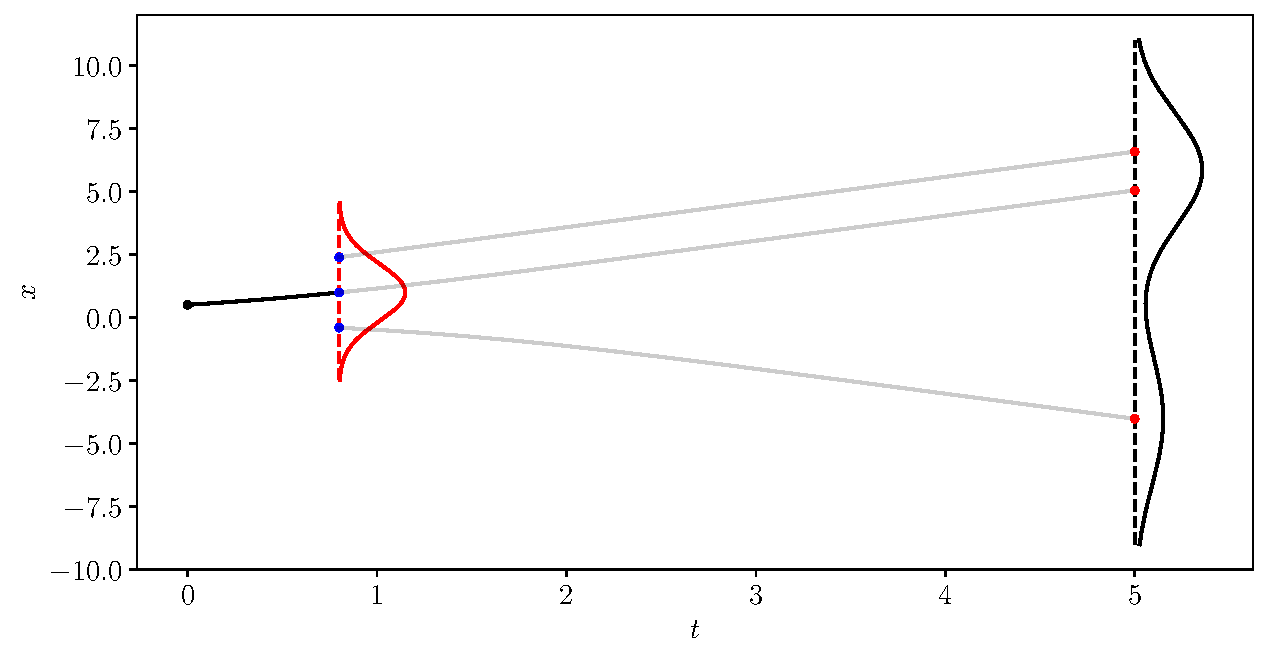
\includegraphics[width=\textwidth]{chp05_gmm/figures/bene_final_gmm_split}
	% 	\caption{An illustration of the algorithm.
	% 	By solving \cref{eqn:gauss_de}, the initial condition \(x_0 = 1/2\) and the corresponding linearisation covariance matrix is propagated forward until \(t = 0.8\) (resulting in the red Gaussian density).
	% 	The mean-covariance pair is then split into three sigma points (in blue), each of which is propagated forward through \cref{eqn:gauss_de}.
	% 	At the final time \(t = 5\), the three mean-covariance pairs for each sigma point describe a Gaussian density, which are combined to produce the final mixture model (in black).}
	% 	\label{fig:bene_gmm_diag}
	% \end{subfigure}
	% \begin{subfigure}{\textwidth}
	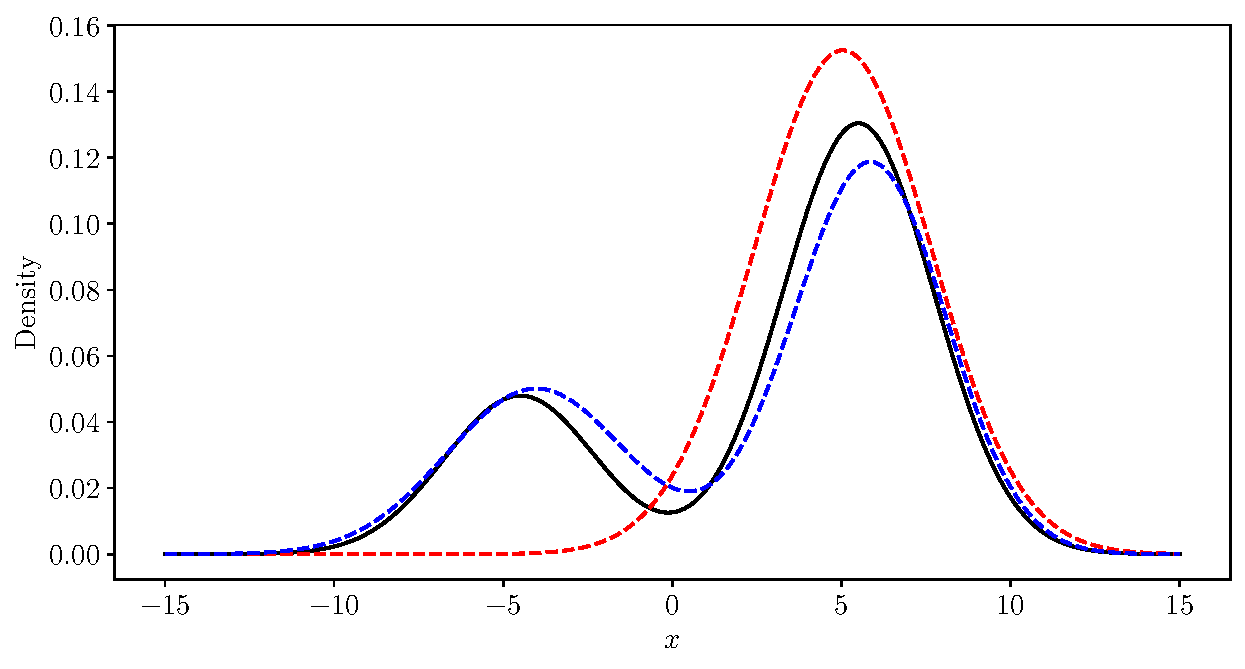
\includegraphics[width=\textwidth]{chp05_gmm/figures/bene_final_gmm}
	% \caption{The probability density function of the solution (in black) to Ben\^e's SDE \cref{eqn:bene_sde} and the corresponding linearisation solution (in dashed red) at time \(T = 5\), with fixed initial condition \(x_0 = 0.5\).
	% The Gaussian mixture model density is overlaid in blue.}
	% \label{fig:bene_gmm_pdf}
	% \end{subfigure}
	\caption{The mixture model algorithm implemented on Ben\^e's SDE \cref{eqn:bene_sde} with fixed initial condition \(x_0 = 0.5\) and over the time interval \((0,5)\).
		The probability density function of the true solution is shown in solid black and the corresponding linearisation solution in dashed red.
		The Gaussian mixture model density is overlaid in blue.
		A single split into three canonical sigma points (using \cref{eqn:uhlman_sigma} occurs at \(t = 0.8\).}
	\label{fig:bene_gmm}
\end{figure}

% \td{Splitting}
% Similar algorithms combining linearisations and mixture models have been proposed, such as that by \citet{DeMarsEtAl_2013_EntropyBasedApproachUncertainty} for propagating an initial uncertainty through a non-linear model, which we compare to.
% However, such algorithms have seen little use in practice, particularly in the oceanography and climate modelling circles.
% In the following chapter (\Cref{ch:appls}), we will demonstrate the mixture model algorithm on examples from these domains.\lb{careful with this paragraph}

\section{The splitting criterion}
In the implementation of our algorithm on Ben\^e's SDE, we manually chose a single split time.
However, in general the algorithm requires a choice of criterion for when to split a Gaussian component, for which there are several choices.
A given Gaussian component should be split when the linearised SDE is no longer a reasonable approximation for the original SDE about the deterministic trajectory corresponding to the component.
This requires an ongoing evaluation of the error in using the approximation.
Some possibilities include:
\begin{itemize}
	\item Alongside the propagation of the mixture model, one can also compute a small number of stochastic samples that solve the original SDE \cref{eqn:sde_y_gmm}.
		These stochastic samples can be compared to the ongoing Gaussian evolutions, for instance using a probabilistic distance measure.
		However, this would increase the computational load of the algorithm and may require many samples to accurately quantify departures from Gaussianity.
	 The Gaussian mixture model does provides an analytic probability density function that can lend itself to further inference, as opposed to solely stochastic samples that require an additional step to compute a density function.
	 There may be a trade-off between the number of samples and the desired computationally efficiency.

	\item A diagnostic based purely on the deterministic model will be computationally efficient, not requiring any stochastic simulation.
		Stochastic sensitivity is a scalar value that is computed directly from the covariance matrix of the Gaussian approximation, and quantifies the magnitude and direction of maximum uncertainty.
		In highly nonlinear systems, stochastic sensitivity may provide a measure for evaluating non-Gaussianity.
		This can be computed from each Gaussian component with minimal additional computational cost, by simply taking the operator norm of the component covariance matrix.
		However, in regions of linearity and non-multiplicative noise, the solution to the SDE can be Gaussian, but stochastic sensitivity, being the magnitude of the noise, can increase.
		A large value of stochastic sensitivity need to imply non-Gaussianity in these cases.


	\item \citet{DeMarsEtAl_2013_EntropyBasedApproachUncertainty} propose an algorithm for propagating an initial uncertainty through a nonlinear time-varying mapping, by using a Gaussian mixture model and a similar splitting algorithm.
The principle is similar to ours; the uncertainty is propagated forward using a linearisation of the model until this is no longer a reasonable approximation.
A split occurs when nonlinearity in the mapping, which would result in non-Gaussianity, is detected via an entropy-based measure.
This measure uses the sigma point method to evaluate the mapping of a covariance matrix, which is compared to the ongoing propagation of a Gaussian component.
The sigma point method provides an \emph{exact} computation for the covariance matrix of a deterministic nonlinear transformation of a random variable, provided that the transformation can be evaluated exactly.
In our case however, there is ongoing uncertainty from the multiplicative noise and the SDE cannot be solved exactly, so we cannot evaluate the mapping required for the sigma point method.
Nonetheless, this previous work may suggest a direction for further tuning the implementation of our method, including the selection of points when splitting a component.

\end{itemize}
We leave further development of this step of the algorithm for future work, and only consider simple demonstrative examples in the next chapter.




% \section{Error remains bounded}
% Our main result of \Cref{ch:linear_theory}, \Cref{thm:main}, establishes that the strong error in approximating the solution to a small-noise nonlinear stochastic differential equation with a linearisation is bounded by a scaling of the initial and ongoing uncertainty scales.
% In this section, we show that this result implies that if we propagate the components of a Gaussian mixture model with linearisations about the component means, as our mixture model algorithm employs, the error remains bounded in a similar fashion.

% Recall the results of \Cref{sec:theory_gauss}, the SDE linearisation theory in the special case of a Gaussian initial condition.
% Suppose that \cref{eqn:sde_no_eps} is subject to a Gaussian initial condition \(x \isGauss{\mu_0, \delta^2\Sigma_0}\), where \(\mu_0 \in \R^n\) and \(\Sigma_0 \in \R^{n\times n}\) are fixed and \(\delta > 0\) is a scaling parameter.
% We can linearise \cref{eqn:sde_no_eps} about the deterministic trajectory \(F_t^0\!\left(\mu_0\right)\) originating from the mean \(\mu_0\), as
% \begin{equation}
% 	\dif l_t\!\left(\mu_0, \delta^2\Sigma_0\right) = \begin{multlined}[t]
% 		\left[F_0^t\!\left(\mu_0\right) + \nabla u\!\left(F_0^t\!\left(\mu_0\right), t\right)\left(l_t\!\left(\mu_0, \delta^2 \Sigma_0\right) - F_0^t\!\left(\mu_0\right)\right)\right]\dif t \\
% 		+ \epsilon\sigma\!\left(F_0^t\!\left(\mu_0\right), t\right)\dif W_t, \quad l\!\left(\mu_0, \delta^2\Sigma_0\right) = x.
% 	\end{multlined}
% 	\label{eqn:scaled_sde_linear}
% \end{equation}
% We have introduced the notation \(l_t\!\left(\mu_0, \delta^2\Sigma_0\right)\) to indicate the dependence of the linearised solution on the initial mean and covariance matrix.
% The solution to \cref{eqn:scaled_sde_linear} at time \(t\) follows a Gaussian distribution with computable mean and covariance, specifically
% \[
% 	l_t\!\left(\mu, \delta^2\Sigma_0\right) \isGauss{F_0^t\!\left(\mu_0\right), \, \delta^2 \nabla F_0^t\!\left(\mu_0\right) \Sigma_0 \left[\nabla F_0^t\!\left(\mu_0\right)\right]^{\T} + \epsilon^2\Sigma_0^t\!\left(\mu_0\right)},
% \]
% where
% \[
% 	\Sigma_0^t\!\left(\mu_0\right) = \nabla F_0^t\!\left(\mu_0\right)\int_0^t{\left[\nabla F_0^\tau\!\left(\mu_0\right)\right]^{-1} \sigma\!\left(F_0^\tau\!\left(\mu_0\right), \tau\right)\sigma\!\left(F_0^\tau\!\left(\mu_0\right), \tau\right)^{\T}\left[\nabla F_0^\tau\!\left(\mu_0\right)\right]^{^{-\intercal}}\dif\tau}\left[\nabla F_0^t\!\left(\mu_0\right)\right]^{\T}.
% \]
% \Cref{thm:main} establishes that for any \(t \in [0,T]\), there exists constants \(A_1(t), A_2(t), A_3(t) \geq 0\) independent of \(\mu_0\) such that
% \begin{equation}\label{eqn:linear_error_bound}
% 	\avg{\norm{y_t - l_t\!\left(\mu_0, \delta^2 \Sigma_0\right)}} \leq A_1(t)\epsilon^2 + A_2(t)\epsilon\delta + A_3(t)\delta^2.
% \end{equation}
% Note that we have dropped the notation indicating the dependence of the constants on the coefficient bounds for notational brevity.
% For completeness, however, we have
% \begin{align*}
% 	A_1(t) & = \left(K_{\nabla\nabla u} + K_{\nabla\sigma}\right)D_1\!\left(1, t, K_{\nabla u}, K_\sigma\right) \\
% 	A_2(t) & = K_{\nabla\nabla u} D_2\!\left(1, t, K_{\nabla u}\right)                                          \\
% 	A_3(t) & = K_{\nabla\sigma}D_3\!\left(1, t, K_{\nabla u}\right),
% \end{align*}
% using the notation of \Cref{thm:main}.
% Suppose at a time \(s \in [0,T]\), we have a mixture model with \(M\) Gaussian components
% \[
% 	p_0\!\left(z\right) = \sum_{i=1}^{M}{\omega_i\Gauss{z;\, \mu_0^{(i)}, \delta^2\Sigma_0^{(i)}}}
% \]
% where \(\omega_1,\dotsc, \omega_M \geq 1\) are weights satisfying \(\sum_{i=1}^M{\omega_i} = 1\), \(\mu_0^{(1)}, \dots \mu_0^{(M)}\) are the component means and \(\Sigma_0^{(1)}, \dotsc, \Sigma_0^{(M)}\) are the component covariance matrices.
% Via linearisation approximations of the form \cref{eqn:scaled_sde_linear}, we construct the mixture model at time \(t > s\)
% \[
% 	p_t\!\left(z\right) = \sum_{i=1}^{M}{\omega_i\Gauss{z; \, F_s^t\!\left(\mu_0^{(i)}\right), \Pi^{(i)}}},
% \]
% where
% \[
% 	\Pi^{(i)} = \delta^2 \nabla F_0^t\!\left(\mu_0\right) \Sigma_0^{(i)} \left[\nabla F_s^t\!\left(\mu_0\right)\right]^{\T} + \epsilon^2 \Sigma_s^t\!\left(\mu_0\right),
% \]
% is the propagated covariance matrix.
% Let \(\Xi_0\) be a random variable distribution distributed according to \(p_0\), which we can write as
% \[
% 	\Xi_0 = \sum_{i=1}^{M}{I_i \xi_0^{(i)}}
% \]
% where \(\xi_0^{(i)} \isGauss{\mu_0^{(i)}, \Sigma_0^{(i)}}\) independently for each \(i\), and \(\left(I_1, \dotsc, I_M\right)\) are a set of indicator variables with
% \[
% 	P\!\left(I_i = 1,\, I_j = 0 \text{ for all } j \neq i\right) = \omega_i,
% \]
% for each \(i = 1,\hdots,M\), and zero probability otherwise.
% Similarly, let \(\Xi_t\) be a random variable distributed according the mixture model \(p_t\), which we construct from solutions to linearised SDEs of the form \cref{eqn:scaled_sde_linear}, by writing
% \[
% 	\Xi_t = \sum_{i=1}^{M}{I_i l_t\!\left(\mu_0^{(i)}, \delta^2\Sigma_0^{(i)}\right)},
% \]
% where each solution to \cref{eqn:scaled_sde_linear} is independent of the others.
% Then, for any \(i\) we have the conditional distribution
% \[
% 	\left. \Xi_t \, | \, \set{I_i = 1, \, I_j = 0 \text{ for all } j \neq i} \right. = l_{t}\left(\mu_0^{(i)}, \delta^2 \Sigma_0^{(i)}\right).
% \]
% The random variable \(\Xi_t\) represents our approximation of the state at time \(t\), after a single step of the mixture model algorithm.
% Via the law of total expectation, the error in approximating \(y_t\) with \(\Xi_t\) is
% \begin{align*}
% 	\avg{\norm{y_t - \Xi_t}} & = \sum_{i=1}^{M}{\avg{\norm{y_t - \Xi_t}\,\middle|\, I_i = 1}}P\!\left(I_i = 1,\, I_j = 0 \text{ for all } j \neq i\right) \\
% 	                         & = \sum_{i=1}^{M}{\omega_i\avg{\norm{y_t - l_{t}\left(\mu_0^{(i)}, \delta^2 \Sigma_0^{(i)}\right)}}}                        \\
% 	                         & = \sum_{i=1}^{M}{\omega_i\left(A_1(t)\epsilon^2 + A_2(t) \epsilon \delta + A_3(t)\delta^2\right)}                          \\
% 	                         & = A_1(t) \epsilon^2 + A_2(t)\epsilon\delta + A_3(t)\delta^2.
% \end{align*}
% In the mixture model algorithm described, the initialising uncertainty (being a component of the mixture model) at each step scales with \(\epsilon\), specifically \(\delta = \epsilon\).
% Thus, the error in the algorithm remains bounded with order \(\epsilon^2\).


% \td{Explain that further theory is needed}

\chapter{An application: drifter in the Gulf Stream}\label{ch:appls}
We now apply the theoretical developments of \Cref{ch:linear_theory} and the mixture model algorithm of \Cref{ch:gmm} to an application using a data-driven model.
We consider a stochastic model constructed from altimetry-derived velocity data of the surface of the Gulf Stream, a climatically important part of the North Atlantic ocean.
This model is 2-dimensional and we construct a deterministic model and use the solving trajectories to approximate the solution to an ``improved'' stochastic counterpart that accounts for measurement error and unresolved effects.
We are able to apply our tools to this model, to provide both qualitative and quantitative insight into the behaviour of the stochastic model and consequently the impact of uncertainty on the deterministic.


\section{The Hellinger distance}
Before moving onto the example, we must first provide a measure to quantitatively evaluate the performance of the Gaussian approximation and our mixture model.
We will use the Hellinger distance, which measures the distance between probability distributions.
% The Hellinger distance is an example of an \(f\)-divergence, a broader class of measures between two probability distributions.
For two continuous probability distributions in \(\R^n\) with respective probability density functions \(p\) and \(q\), the Hellinger distance between the two distributions is given by \citep{LeCamLoYang_2000_AsymptoticsStatistics}
\begin{equation}\label{eqn:hell_dist}
	D_H\!\left(p, q\right) = \sqrt{\frac12 \int_{\R^n}{\left(\sqrt{p(x)} - \sqrt{q(x)}\right)^2\dif x}} = \sqrt{1 - \int_{\R^n}{\sqrt{p(x)q(x)}\dif x}}.
\end{equation}
We previously discussed (in \Cref{sec:comparison}) the Kullback-Leibler divergence---this measure was used by \citet{Sanz-AlonsoStuart_2017_GaussianApproximationsSmall} to quantify the performance of Gaussian approximations to SDE solutions---but opt to use the Hellinger distance.
There are several attractive properties of the Hellinger distance: the Hellinger distance is defines a metric on the space of probability measures and always takes values in the interval \([0,1]\), unlike the KL-divergence which is not a formal metric and can become infinite.

Since the models we will be working with cannot be solved exactly, we will use stochastic samples as our ground `truth`, obtained either via a numerical solver (in the case of SDEs) or Gillespie simulation (in the case of population processes).
That is, without access to the true solutions to our model, we instead take a large number of stochastic samples and compare our approximations to those.
This fits in with the philosophy of our aims; the stochastic sampling approach is the standard in practice, and we seek approximations that give the same conclusions without the computational expense.

However, using stochastic samples presents a complication in using \cref{eqn:hell_dist} to compute the Hellinger distance: the calculation requires evaluation of the probability density function from which these realisations were sampled.
This would require a choice for how to approximate the density function and then compute the integral in \cref{eqn:hell_dist}; one option is to construct a kernel density estimator, where a certain known distribution (usually a Gaussian with a small variance) is placed at each realisation and then combined into a mixture density.
To avoid the need to make such a choice, we will instead use an \emph{empirical} estimator that approximates \cref{eqn:hell_dist} purely from samples and without having to evaluate either probability density function.
Although we will be comparing the numerical realisations to analytically available probability density functions (from either a single Gaussian approximation of the mixture model algorithm---the availability of the PDFs is another advantage of these methods over Monte-Carlo simulation), we will generate samples from both distributions to use a purely empirical estimator.
We will employ the empirical estimator proposed by \citet{DingMullhaupt_2023_EmpiricalSquaredHellinger}, which extends a similar estimator for the KL-divergence by \citet{Perez-Cruz_2008_KullbackLeiblerDivergenceEstimation}. % to a broader class of divergences, including the Hellinger distance.
Let \(\set{\hat{x}_1, \dotsc, \hat{x}_N}\) and \(\set{\hat{y}_1, \dotsc, \hat{y}_N}\) denote the two sets of realisations from the probability density functions \(p\) and \(q\) respectively.
The estimator is first computed as
\begin{equation}\label{eqn:hell_emp_Ha}
	\hat{H}_a^2\!\left(p, q\right) = 1 - \frac{\sqrt{N - 1}\,\Gamma\!\left(k\right)^2}{N^{3/2}\,\Gamma\!\left(k - \frac12\right)\Gamma\!\left(k + \frac12\right)} \sum_{i=1}^{N}\frac{r_k\!\left(x_i\right)^{n/2}}{s_k\!\left(\hat{x}_i\right)^{n/2}}
\end{equation}
where \(\Gamma\) denotes the Gamma function, and \(r_k\!\left(\hat{x}_i\right)\) and \(s_k\!\left(\hat{x}_i\right)\) denote the Euclidean distance to the \(k\)th nearest neighbour of \(\hat{x}_i\) in \(\set{\hat{x}_1, \dotsc, \hat{x}_N} \setminus \set{\hat{x}_i}\) and \(\set{\hat{y}_1, \dotsc, \hat{y}_N}\) respectively.
The parameter \(k\) is the number of neighbouring points used to construct a \(k\)-nearest-neighbour density estimate as an intermediate step in the calculation.
The value of \(k\) is specified in advance, and we take \(k = 5\) throughout to ensure a reasonable computation time.
This provides a consistent (in the sense of almost sure convergence in the limit of infinite sample size \(N\)) estimator of the squared Hellinger distance \citep{DingMullhaupt_2023_EmpiricalSquaredHellinger}.
However, \cref{eqn:hell_emp_Ha} is not symmetric in \(p\) and \(q\), i.e. \(\hat{H}_a^2\!\left(p,q\right) \neq \hat{H}_a^2\!\left(q,p\right)\) with the asymmetry arising in the distances \(r_k\) and \(s_k\).
In practice, one direction can provide a more accurate estimator depending on the nature of the underlying distributions from which the samples are taken.
To ensure symmetry in the final estimate and find a `middle ground` between the two asymmetric estimators, \citet{DingMullhaupt_2023_EmpiricalSquaredHellinger} propose taking the average:
\begin{equation}\label{eqn:hell_emp}
	\hat{H}\!\left(p,q\right) = \sqrt{\frac{\hat{H}_a^2\!\left(p,q\right) + \hat{H}_a^2\!\left(q,p\right)}{2}},
\end{equation}
which still exhibits the same convergence properties of \(\hat{H}_a\).
Note that this estimator is random, as it relies upon samples from both densities.
We therefore take multiple realisations of \(\hat{H}\), each using a new set of samples, and use the average to reduce the variance in the estimator.

% For two discrete distributions \(\hat{P}\) and \(\hat{Q}\) defined on the same support with respective probability mass functions \(p_1, p_2, \dotsc, p_K\) and \(q_1, q_2, \dotsc, q_K\), the Hellinger distance is
% \begin{equation}\label{eqn:hell_disc}
% 	D_H\!\left(\hat{P}, \hat{Q}\right) = \sqrt{\frac12 \sum_{i=l}^{K}\left(\sqrt{p_i} - \sqrt{q_i}\right)^2}
% \end{equation}
% The Hellinger distance is symmetric and defines a metric on the space of probability distributions.
% We will use the Hellinger distance to compare three estimates of the solution to a stochastic differential equations: numerical samples from a numerical solver, analytic probability density functions from the linearised approximation and Gaussian mixture model algorithm, and a spatially discretised solution to the Fokker-Planck equation.
% This presents an ambiguity in whether to use the continuous or discrete definition of the Hellinger distance.
% We choose to use the discrete definition, by discretising the continuous probability denisity and computing an empirical probability mass function from the samples.
% The state space is divided into \(K\) non-overlapping bins \(b_1, b_2, \dotsc, b_K \subset \R^n\).
% Given \(N\) samples, the empirical probability corresponding to a bin is the proportion of samples that fall within that bin.
% For a continuous random variable \(X\) with probability density function \(p_c\), the probability of \(X\) falling inside a bin \(b_i\) is given by
% \[
% 	P\!\left(X \in b_i\right) = \int_{b_i}{p_c(x)\dif x}.
% \]
% For multivariate Gaussian and Gaussian mixture model densities, this integral cannot be evaluated exactly, so instead we use a Monte-Carlo estimate.
% We generate a large number of samples from the density, and compute the proportion of samples that fall in each bin.
% With two empirical PMFs constructed over the same set of bins, we can then compute the Hellinger distance between the two using the discrete formulation \cref{eqn:hell_disc}.
% This is a \emph{n\"aive} approach to estimating the Hellinger distance and there are alternative methods available (e.g. the empirical estimate recently proposed by \citet{DingMullhaupt_2023_EmpiricalSquaredHellinger}), but these methods only work in 1-dimension, whereas we will be dealing with 2- and 5-dimensional samples and probability density functions in this chapter.\lb{Gotta rewrite this sentence man, and check that the dimensionality really is an issue.}


% \subsection{The Wasserstein metric}
% To evaluate the performance of our mixture model and compare to other approaches (such as stochastic simulation), we require a measure that compares probability distributions.
% The Wasserstein distance (also known as the earth mover's distance) is one such metric between probability distributions.
% The Wasserstein \(p\)-distance, for \(p \geq 1\), is defined formally as follows.
% Let \(\mu\) and \(\nu\) denote two probability measures on \(\R^n\), each with finite \(p\)-moments.
% Then, the Wasserstein \(p\)-distance between \(\mu\) and \(\nu\) is
% \[
% 	W_p\!\left(\mu, \nu\right) = \left(\inf_{\gamma \in \Gamma\!\left(\mu, \nu\right)}\mathds{E}_{(x,y) \in \gamma}\!\left[\norm{x - y}^p\right]\right)^{1/p},
% \]
% where \(\Gamma\!(\mu, \nu)\) is the set of all couplings of \(\mu\) and \(\nu)\).
% A coupling \(\gamma\) between \(\mu\) and \(\nu\) is a probability measure on \(\R^n \times \R^n\) such that the marginals are \(\mu\) and \(\nu\), i.e.
% \begin{align*}
% 	\int_{\R^n}{\gamma(x,y)\dif y} & = \mu(x), \\
% 	\int_{\R^n}{\gamma(x,y)\dif x} & = \nu(y).
% \end{align*}
% If \(\mu\) and \(\nu\) admit the respective probability density functions \(p, q \colon \R^n \to [0,\infty)\), then the Wasserstein distance can be written as
% \[
% 	W_p\!\left(p, q\right) = \left(\inf_{\gamma \in \Gamma\!\left(p,q\right)}\int_{\R^n \times \R^n}{\norm{x - y}^p \gamma\!\left(x,y\right)\dif x\dif y}\right)^{1/p}.
% \]




% \begin{figure}
% 	\begin{center}
% 		% \includegraphics[width=\textwidth]{}
% 		\caption{An example of a coupling between two probability density functions (plotted on each axes) on \(\R\).
% 			A coupling is a joint distribution from which the two individual distributions are recovered from the marginals, and is not unique.
% 			The Wasserstein distance is computed by taking an infimum across the set of all possible couplings.}
% 		\label{fig:pdf_coupling}
% 	\end{center}
% \end{figure}






\section{Model setup}\label{sec:appl_ocean}
% For our first application, we consider a oceanographic model derived from satellite-observed velocity data of part of the Gulf Stream.
The Gulf Stream is a warm water current that originates in the Gulf of Mexico and travels through the North Atlantic, and plays a vital role in climate patterns in the Northern and Western hemispheres \citep{Palter_2015_RoleGulfStream}.
The stream itself consists of a rapidly-moving jet which varies dramatically with time, and small eddies of warm water that are formed and shed from the stream \citep{KangCurchitser_2013_GulfStreamEddy}.
The Gulf Stream is a well-studied region of the ocean, due to the climatic importance and the interesting dynamical behaviour exhibited by the flow.

Consider tracking the longitudinal and latitudinal position of a drifter travelling on the surface of the ocean.
We construct a differential equation for the time-evolution of the drifter position from geostrophic velocity data inferred from altimetry (sea surface height) observations by satellite.
The dataset is supplied by the \citet{E.U.CopernicusMarineServiceCMEMS_2020_GlobalOceanGridded} and has been processed by the Data Unification and Altimeter Combination System (DUACS).
The sea surface height is proportional to the streamfunction for the surface flow, provided that the flow is treated as two-dimensional, with a constant of proportionality that varies with latitude \citep{Park_2004_DeterminationSurfaceGeostrophic,DoglioniEtAl_2021_SeaSurfaceHeight}.
This enables approximation of the zonal (eastwards) and meridional (northwards) geostrophic velocities, which are given in metres per second.
These measurements are taken hourly and available on a \(0.25^\circ \times 0.25^\circ\) spatial grid.
We convert the measured velocities to degrees per day via the following transformation: at longitude \(\lambda\) and latitude \(\phi\) (both in degrees), the components \(u_{\mathrm{m}}\) and \(v_{\mathrm{m}}\) in metres per second are transformed as \citep{Capderou_2014_HandbookSatelliteOrbits}
\begin{subequations}\label{eqn:natl_vel_conv}
	\begin{align}
		u\!\left(\lambda, \phi, t\right) & = \frac{1 - \left(2f - f^2\right)^2}{a}\left(1 - \left(2f - f^2\right)^2\sin^2\!\left(\phi\right)\right)^{3/2} u_{\mathrm{m}}\!\left(\lambda, \phi, t\right) \\
		v\!\left(\lambda, \phi, t\right) & = \frac{1}{a\cos\!\left(\phi\right)}\left(1 - \left(2f - f^2\right)^2\sin^2\!\left(\phi\right)\right)^{1/2} v_{\mathrm{m}}\!\left(\lambda, \phi, t\right),
	\end{align}
\end{subequations}
where \(a\) is the semi-major axis and \(f\) the flattening of an ellipsoid model of the Earth.
We use the World Geodesic System 84, which gives the values \citep{Capderou_2014_HandbookSatelliteOrbits}
\[
	a = 6378137\,\unit{\metre}, \quad f = 1 / 298.257223563.
\]
Although the dataset provides global coverage, we focus our attention on the longitudes between \(-66^\circ\)E and \(-52^\circ\) and \(34^\circ\)N and \(46^\circ\), and measurements starting from midnight \DTMdisplaydate{2020}{01}{01}{-1}.
We use a larger spatial subset for calculations, however, to prevent issues at the boundaries of the spatial domain.
There is a region of land---a small part of the south-east coast of Canada---in the dataset, where velocity data is missing.
We set the velocity to zero in this region, as we know from physical considerations that the drifter could not travel on land, and in all following figures indicate this region with black.

% Suppose we have the sea surface height (SSH) \(\eta = \eta\left(\lambda, \phi, t\right)\) at longitude \(\lambda\) and latitude \(\phi\) (both in radians), and at time \(t\).
% The SSH \(\eta\) is then proportional to the streamfunction for the surface flow, if we treat the surface flow as two-dimensional, where the constant of proportionality varies with latitude \citep{Park_2004_DeterminationSurfaceGeostrophic, DoglioniEtAl_2021_SeaSurfaceHeight}.
% The geostrophic zonal (east-west) and meridional (north-south) velocities \(u\) and \(v\) are then given by
% \begin{subequations}\label{eqn:}
% 	\begin{align}
% 		u\left(\lambda, \phi, t\right) & = -\frac{g}{f\left(\phi\right)}\dpd{\eta}{\phi} \label{eqn:altimetry_u}    \\
% 		v\left(\lambda, \phi, t\right) & = \frac{g}{f\left(\phi\right)}\dpd{\eta}{\lambda} \label{eqn:altimetry_v},
% 	\end{align}
% \end{subequations}
% \label{eqn:altimetry_uv}
% where
% \[
% 	f\left(\phi\right) = 2\Omega_{\mathrm{r}}\sin{\phi}
% \]
% is the Coriolis parameter, \(g \approx 9.81\mathrm{\,m\,s}^{-1}\) is the standard acceleration due to gravity, and \(\Omega_\mathrm{r} \approx 7.2921 \times 10^{-5}\mathrm{\,radians\,s}^{-1}\) is the rotation rate of the Earth.
% \Cref{fig:na_motive_flow} provides snapshots of the absolute geostrophic speed and contours of the sea-surface height, at times chosen to exhibit the formation and separation of an eddy from the main stream.
% The sea-surface height contours correspond to the instantaneous streamfunction of the flow.
% Although the Eulerian snapshots of the velocity data provide some indication of this behaviour, it is important to note that this data is often not sufficient to fully understand the dynamics; the movement of solving (Lagrangian) trajectories provide insight into the time-evolving behaviour of the system.
% \td{The figure caption is a lie; what behaviour is being shown? Why this time span? May need to go for even longer to see anything interesting :(.}

% \begin{figure}
% 	\begin{center}
% 		\begin{subfigure}{0.49\textwidth}
% 			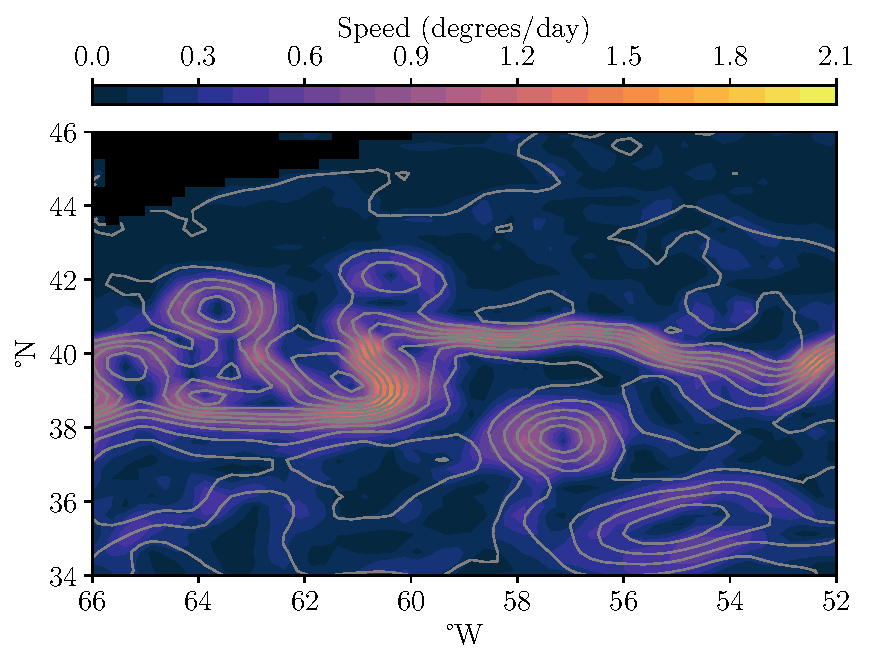
\includegraphics[width=\textwidth]{chp06_applications/figures/gulf_stream/streamlines_0}
% 			\caption{\(t = 0\) (midnight \DTMdisplaydate{2020}{01}{01}{})}
% 		\end{subfigure}
% 		\begin{subfigure}{0.49\textwidth}
% 			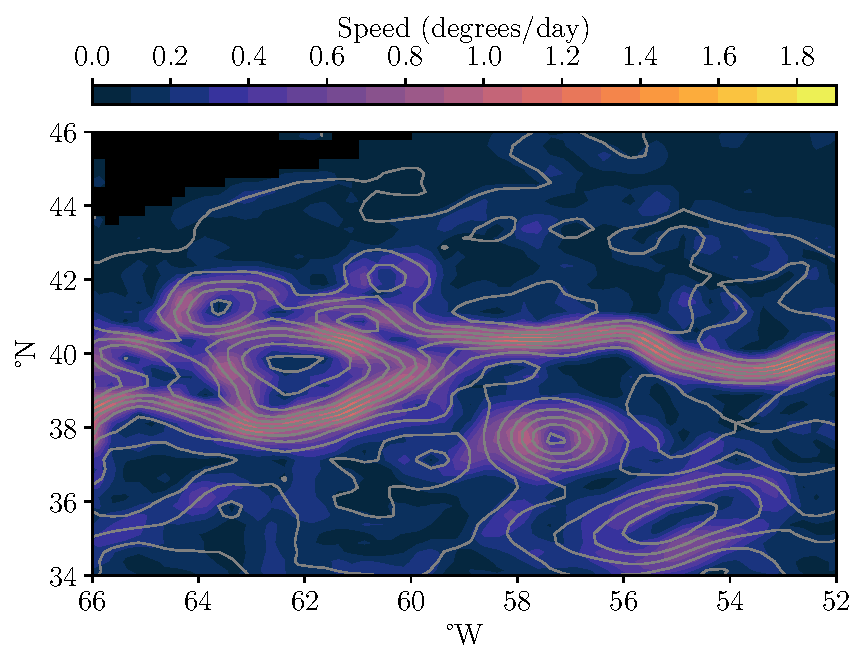
\includegraphics[width=\textwidth]{chp06_applications/figures/gulf_stream/streamlines_5}
% 			\caption{\(t = 5\) (midnight \DTMdisplaydate{2020}{01}{6}{})}
% 		\end{subfigure}
% 		\begin{subfigure}{0.49\textwidth}
% 			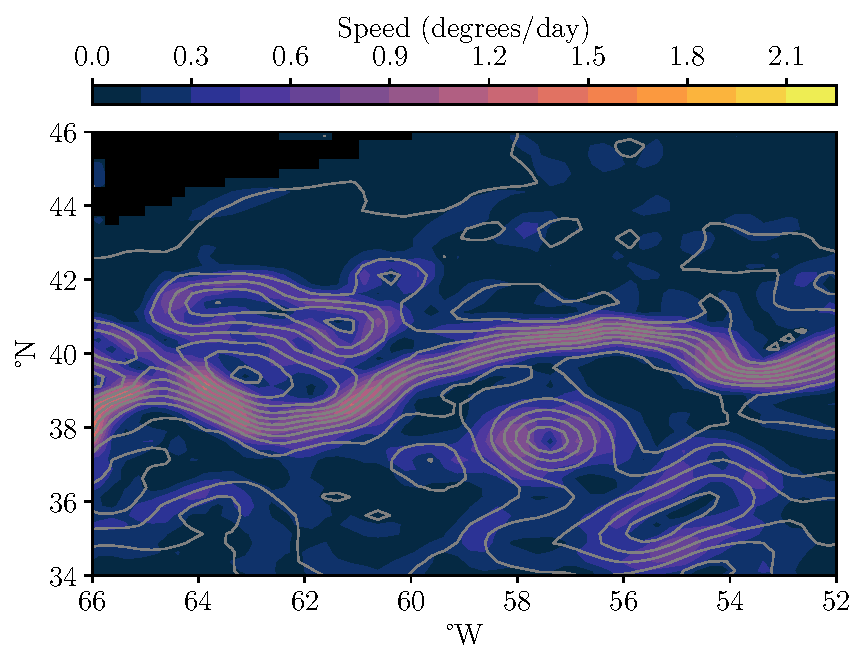
\includegraphics[width=\textwidth]{chp06_applications/figures/gulf_stream/streamlines_10}
% 			\caption{\(t = 10\) (midnight \DTMdisplaydate{2020}{01}{11}{})}
% 		\end{subfigure}
% 		\begin{subfigure}{0.49\textwidth}
% 			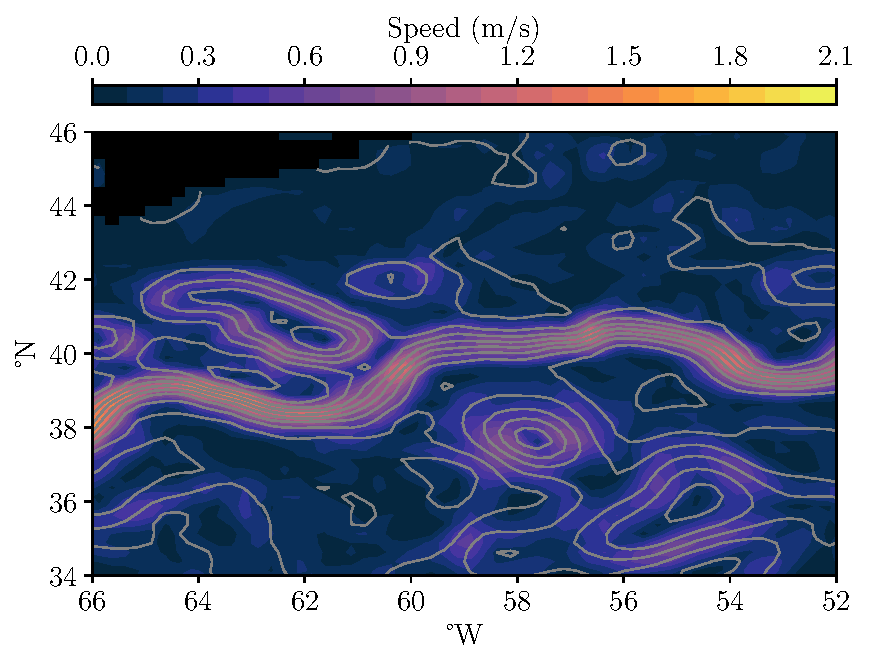
\includegraphics[width=\textwidth]{chp06_applications/figures/gulf_stream/streamlines_15}
% 			\caption{\(t = 15\) (midnight \DTMdisplaydate{2020}{01}{16}{})}
% 		\end{subfigure}
% 		\caption{The absolute surface current speed (coloured) and contours of the sea-surface height (streamlines of the flow, in grey) of the Gulf Stream dataset, at various times chosen to demonstrate the formation and separation of an eddy from the stream.
% 			The black region indicates missing data, due to the presence of land.
% 			All times are in Greenwich Mean Time.}
% 		\label{fig:na_motive_flow}
% 	\end{center}
% \end{figure}

\begin{figure}
	\centering
	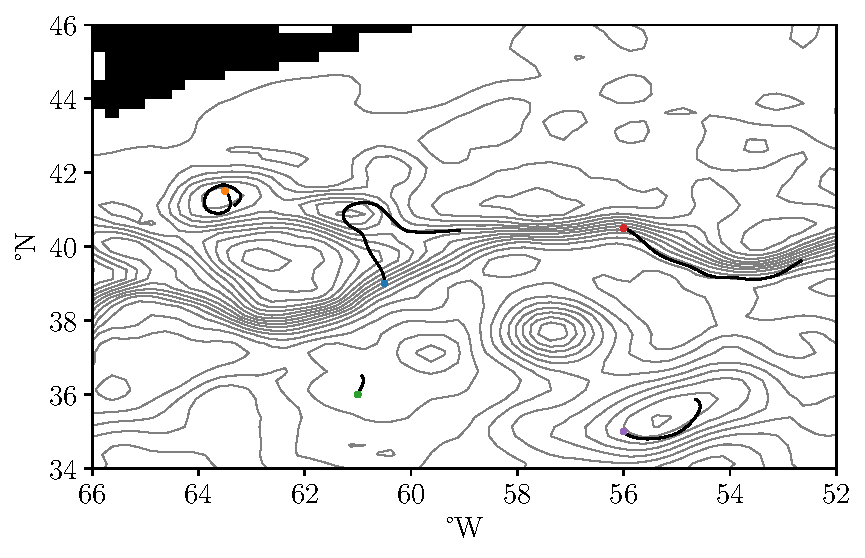
\includegraphics[width=\textwidth]{chp06_applications/figures/gulf_stream/det_trajs}
	\caption{Several trajectories that solve \cref{eqn:natl_ode} and describe the motion of drifters on the surface of the Gulf Stream.
		Each trajectory is initialised at a coloured point at \(t = 0\) (midnight \DTMdisplaydate{2020}{1}{1}{}), and evolved by numerically solving \cref{eqn:natl_ode} up to midnight \(t = 7\) (midnight \DTMdisplaydate{2020}{1}{8}{}).}
	\label{fig:natl_ode_sols}
\end{figure}

The velocity data is Eulerian and unsteady (varying with time), so to predict the position of a drifter we must solve for a Lagrangian trajectory.
This first requires interpolating the velocity data between the spatial and temporal gridpoints, for which we use a linear interpolate.
Let \(x_t \equiv \left(x_t^{(\mathrm{lon})}, x_t^{(\mathrm{lat})}\right)^{\T}\) denote the longitudinal (in degrees east) and latitudinal (in degrees north) position of the drifter \(t\) days after midnight \DTMdisplaydate{2020}{01}{01}{-1}.
The deterministic model for \(x_t\), constructed purely from the interpolated velocity data, is
\begin{equation}\label{eqn:natl_ode}
	\dod{}{t}\begin{bmatrix}
		x_t^{(\text{lon})} \\ x_t^{(\text{lat})}
	\end{bmatrix} = \begin{bmatrix}
		\tilde{u}\!\left(x^{(\mathrm{lon})}_t, x^{(\mathrm{lat})}_t, t\right) \\ \tilde{v}\!\left(x^{(\mathrm{lon})}_t, x^{(\mathrm{lat})}_t, t\right)
	\end{bmatrix},
\end{equation}
where \(\tilde{u}\) and \(\tilde{v}\) are the interpolated zonal and meridional velocities respectively.
\Cref{fig:natl_ode_sols} shows some example trajectories that solve \cref{eqn:natl_ode}, evolving over the span of a week.
Contours of the sea surface height at \(t = 8\) are also shown in grey, which correspond to those of the instantaneous streamfunction and provide an indication of the flow structure.
The stream itself is fast-moving and a prominent feature of the flow, and consequently drifters starting (e.g. the blue and red points) within the stream are transported along it.
Along the stream, eddies form and break off (roughly indicated by the circular regions in the sea-surface height contour map), and trajectories that start within eddy (orange and purple points) typically remain there.
Away from the stream and the eddies, the flow is relatively isotropic and slow-moving, resulting in the short and fairly unremarkable trajectory from the green point.

\begin{figure}
	\centering
	\begin{subfigure}{0.49\textwidth}
		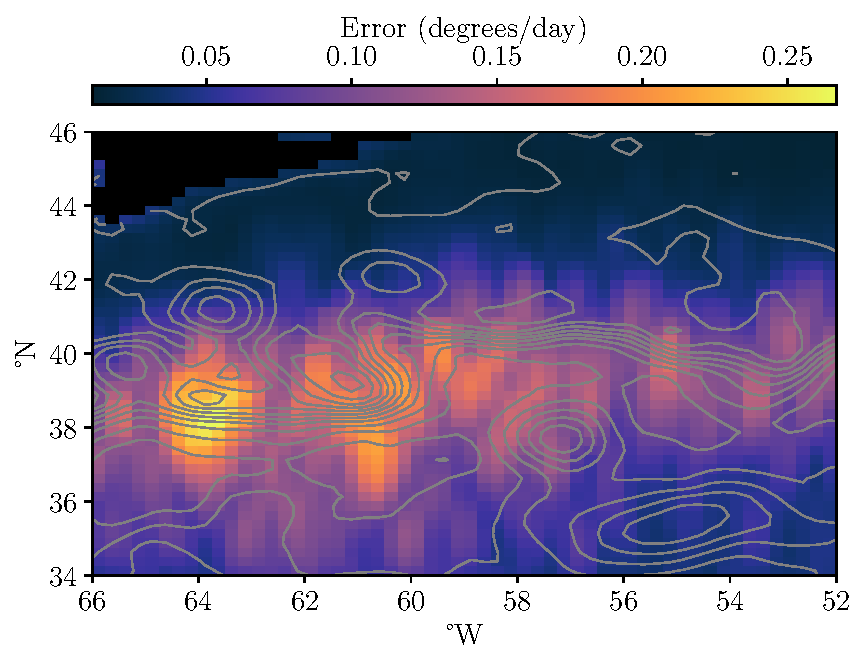
\includegraphics[width=\textwidth]{chp06_applications/figures/gulf_stream/u_err_0}
		\caption{Zonal component}
	\end{subfigure}
	\begin{subfigure}{0.49\textwidth}
		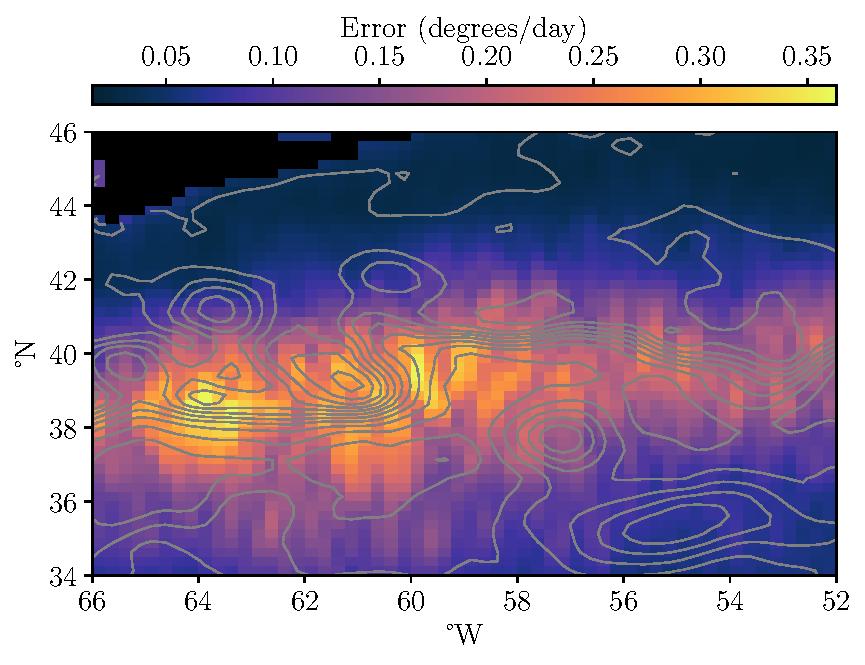
\includegraphics[width=\textwidth]{chp06_applications/figures/gulf_stream/v_err_0}
		\caption{Meridional component}
	\end{subfigure}
	\caption{The mapping error in the (a) zonal (longitudinal) and (b) meridional velocity components at midnight \DTMdisplaydate{2020}{01}{01}{-1} (\(t = 0\)).}
	\label{fig:natl_err}
\end{figure}

We may think of \cref{eqn:natl_ode} as our ``best available'' deterministic model for the time-evolution of the drifter position; if the data (and the subsequent interpolation) were exactly correct, then \cref{eqn:natl_ode} would provide accurate predictions.
However, this is certainly not the case and there are many sources of uncertainty not accounted for by using \cref{eqn:natl_ode} alone.
The dataset additionally includes estimates for the mapping error (an estimate of the variance) in the zonal and meridional velocity measurements, and in particular provides an indication of measurement error. %; typically the error is smaller in regions directly under satellite tracks.
The mapping error in each velocity component at \(t = 0\) is shown in \Cref{fig:natl_err}, as an example of the structure of the field, along with contours of the sea surface height.
The error varies with time, but retains the main structure in that it appears highest along the Gulf Stream and features a stratified appearance due to the fact that satellite measurements are more accurate directly under the tracks followed by the instruments\lb{Check this!!}.%, which is not unexpected as this region contains the most complicated part of the flow.
We can capture both the spatial and temporal variation in this mapping error by adding multiplicative noise to the deterministic model \cref{eqn:natl_ode}.
To account for measurement error, we use the following stochastic model:
\begin{equation}
	\dif \begin{bmatrix}
		x^{(\mathrm{lon})}_t \\ x^{(\mathrm{lat})}_t
	\end{bmatrix} = \begin{multlined}[t]
		\begin{bmatrix} \tilde{u}\!\left(x^{(\mathrm{lon})}_t, x^{(\mathrm{lat})}_t, t\right) \\ \tilde{v}\!\left(x^{(\mathrm{lon})}_t, x^{(\mathrm{lat})}_t, t\right) \end{bmatrix}\dif t \\
		+ \sqrt{L_r}\begin{bmatrix}
			\sqrt{\tilde{u}_{\mathrm{err}}\!\left(x^{(\mathrm{lon})}_t, x^{(\mathrm{lat})}_t, t\right)} & 0                                                                                           \\
			0                                                                                           & \sqrt{\tilde{v}_{\mathrm{err}}\!\left(x^{(\mathrm{lon})}_t, x^{(\mathrm{lat})}_t, t\right)}
		\end{bmatrix} \dif W_t,
	\end{multlined}
	\label{eqn:natl_sde}
\end{equation}
where \(\tilde{u}_{\mathrm{err}}\) and \(\tilde{v}_{\mathrm{err}}\) are the interpolated error estimates for the zonal and meridional velocities (converted to degrees per day using the same transformation \cref{eqn:natl_vel_conv} as was done on the velocity data), and \(L_r = 0.25^\circ\) is the spatial resolution of the data.
Our choice for the diffusion matrix \(\sigma\) comes from the intuition that \(L_r\sigma\sigma^{\T}\) represents the instantaneous variance of the noise in our stochastic differential equation and to ensure that the units in \cref{eqn:natl_sde} are consistent with the convention that \(\dif W_t \sim \sqrt{\mathrm{days}}\) \citep{Oksendal_2003_StochasticDifferentialEquations}.
Both coefficients depend on time and the noise is multiplicative, making \cref{eqn:natl_sde} the most general type of SDE that our theory is equipped to handle.
In our framework of a small noise SDE \cref{eqn:sde_y}, we have set \(\epsilon = 0.25\) and treat this value as being fixed by the data and model.
The introduction of noise in \cref{eqn:natl_sde} can improve over \cref{eqn:natl_ode} by accounting for both the data-informed measurement error and unresolved behaviours between gridpoints, in the fashion of stochastic parameterisation.
This is, however, only one choice for such a model, and a simple one for the purposes of our work.
The same analysis and we are about to conduct could be applied to a better informed stochastic model.




% The derivatives \(\nabla u\) of the deterministic velocity field in \cref{eqn:natl_sde} are approximated via the centred finite-differences,
% \begin{align*}
% 	\dpd{u\left({x^{(\text{lon})}}, {x^{(\text{lat})}}, t\right)}{{x^{(\text{lon})}}} & \approx \frac{u\left(x^{(\text{lon})} + L_r, x^{(\text{lat})}, t\right) - u\left(x^{(\text{lon})} - L_r, x^{(\text{lat})}, t\right)}{2 L_r},
% \end{align*}
% and similar for the remaining derivatives.



% We will now introduce an example of a differential equation model constructed from observed data, which we will use throughout this chaper, and explore further in \Cref{ch:appls}.
% In particular, the technical details of this example will be provided in \Cref{sec:appl_ocean}.

% Suppose we are interested in tracking the position of a drifter on the surface of the Gulf Stream.
% The only information we have available are measurements of the eastwards (zonal) and northwards (meridional) velocities at the surface, derived from altimetry (sea surface height) data.
% Such data is available from the European Commission`s Copernicus Marine Environment Monitoring Service.

% For the purposes of this example, assume that the position of the drifter at the initial time is known exactly\footnote{In practice, of course, this will not be the case, but this will introduce even more uncertainty into our model, furthering reinforcing the purpose of this example.}.
% Assuming that the interpolated data provided an accurate model of the sea surface velocity, the position \(x_t\) of the drifter on the surface at time \(t\) is the solution to the ordinary differential equation
% \begin{equation}\label{eqn:na_motiv_ode}
% 	\dod{x_t}{t} = u\left(x_t, t\right),
% \end{equation}
% subject to the known initial position \(x_0\), where \(u\) is the appropriately interpolated surface velocity data.
% To illustrate the time-varying dynamics of the Stream, \Cref{fig:na_motiv_flow} plots contours the sea-surface height, which correspond to the time-varying streamfunction of the flow, and therefore solutions to \cref{eqn:na_motiv_ode}, at various times.
% An important feature of the flow is that there are significantly different qualitative regimes; there is the rapidly moving stream itself, the eddies that are shed and slow moving, and isotropic regions in between where the current is comparatively slow.



% We can easily solve \cref{eqn:na_motiv_ode} numerically to obtain a predicted position for our drifter on day \(t\).
% % We term \cref{eqn:na_motiv_ode} the \emph{deterministic model}, since given the data we have available, it serves as our best purely deterministic model for the position of the drifter.
% Suppose that our drifter begins within the stream itself, at \(x_0 = \left(-60.5, 39\right)^{\T}\), \Cref{fig:na_motiv_det} plots the resulting trajectory (in white) obtained by solving \cref{eqn:na_motiv_ode} numerically, over the span of 7 days starting from midnight \DTMdisplaydate{2020}{01}{01}{}.
% Based on this model, we expect that the drifter will follow the Stream, which can inform efforts to locate the drifter.

% \begin{figure}
% 	\begin{center}
% 		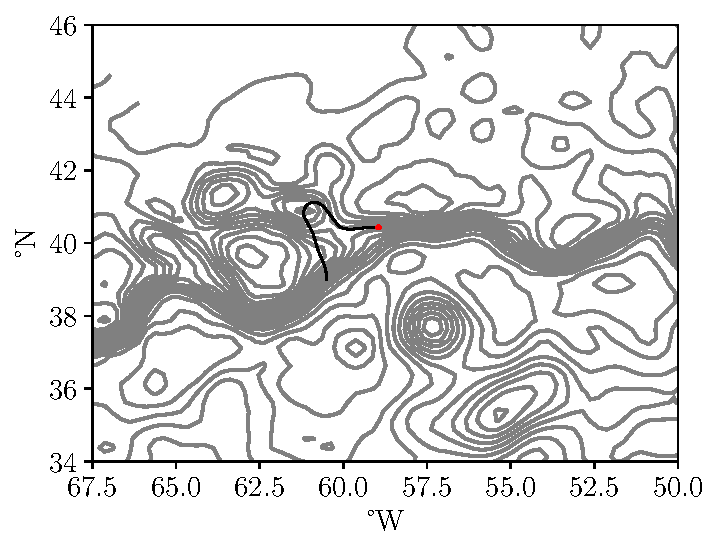
\includegraphics[width=\textwidth]{chp06_applications/figures/gulf_stream_motivation/det_traj.pdf}
% 		\caption{The time evolution of the solution (obtained by numerically integrating the velocity data) to the deterministic system corresponding to \cref{eqn:natl_sde}, from initial condition \(x_0 = \left(-60.5, 39\right)^{\T}\) from 01/01/2021 (\(t = 0\)) to 08/01/2021 (\(t = 8\)).
% 			Contours of the sea surface height at the final time \(t = 8\) are included in grey to indicate the position of the Gulf Stream and nearby eddies in the flow.}
% 		\label{fig:na_motiv_det}
% 	\end{center}
% \end{figure}

% To improve our predictions of the future position of the drifter, we should attempt to account for this uncertainty in our model \cref{eqn:na_motiv_ode}.
% The altimetry-derived data also includes measures of error in each component of the velocity at each spatiotemporal gridpoint, so we can use these measurements to model the ongoing observational error in \(u\).
% We can extend \cref{eqn:na_motiv_ode} as a stochastic differential equation, where the unresolved uncertainty is parameterised as a white-noise process scaled by measurement error.
% Specifically, we formulate the drifter position as \cref{eqn:natl_sde} in \Cref{sec:gulf_stream}, which is explained in more detail in that section.
% For our purposes here, \cref{eqn:natl_sde} is a stochastic differential equation analogy of \cref{eqn:natl_sde} that we can solve numerically to obtain approximate solution samples.

% \Cref{fig:na_motiv_rels} shows us the result of numerically solving a stochastic differential equation formulation (specifically ) of the Lagrangian trajectory model.
% This is a ``more correct'' model than the deterministic counterpart, in the sense that it is attempting to account for the unknowable measurement error and unresolved subgrid effects.
% Each realisation here could correspond to our drifter, and we see a far different picture than the deterministic model alone provided.
% Qualitatively, rather than following the Stream itself, a proportion of particles are caught in one of two eddies which have formed and broken off from the Stream.

% \begin{figure}
% 	\begin{center}
% 		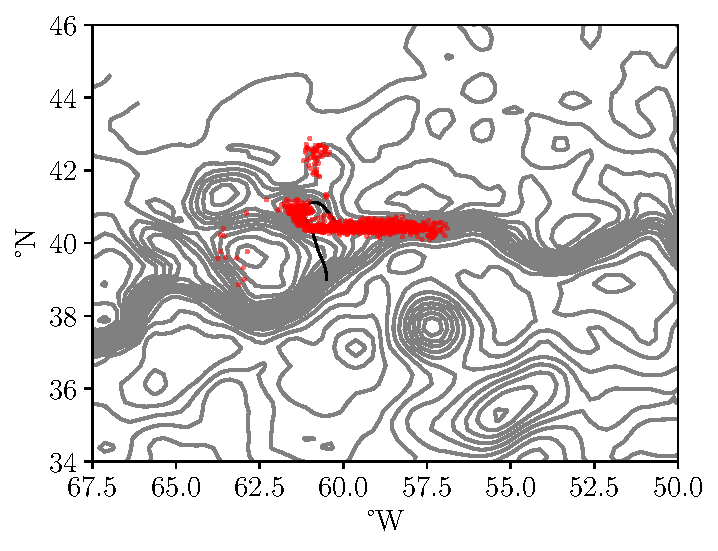
\includegraphics[width=\textwidth]{chp06_applications/figures/gulf_stream_motivation/num_rels.pdf}
% 		\caption{The same visualisation of the deterministic behaviour of the Gulf Stream example as \Cref{fig:na_motive_det}, but with the final positions of 10000 numerical realisations of a stochastic model, each indicated by a red point.}
% 		\label{fig:na_motiv_rels}
% 	\end{center}
% \end{figure}

% Although deterministic models are often easier to work with analytically and far more efficient to solve numerically, these models are limited.
% By explicitly accounting for uncertainty with a stochastic, we can expand the scope of our model and provide more realistic and useful predictions, at the cost of a more complicated model.
% This idea of introducing stochastic components into a deterministic model to account for unresolved and unknown aspects has been used extensively in recent times across scientific applications, notably atmospheric, climate, and oceanographic modelling.
% We provide an overview of this so-called stochastic parameterisation in the next section, and highlight how the work of this thesis fits in with the needs of that field.

\section{Stochastic sensitivity}
We first compute the stochastic sensitivity field.
As in \Cref{sec:comput_s2} of \Cref{ch:linear_numerics}, the purpose of this example is to demonstrate the computation of stochastic sensitivity from the covariance matrix, rather than provide any new insight.
A similar example of computing the stochastic sensitivity field for a similar sea-surface dataset of the Gulf Stream, albeit using the original method of calculation \citep{Balasuriya_2020_StochasticSensitivityComputable}, is provided by \citet{BadzaEtAl_2023_HowSensitiveAre}.

\begin{figure}
	\centering
	\begin{subfigure}{\textwidth}
		\includegraphics[width=0.49\textwidth]{chp06_applications/figures/gulf_stream/S2_field_grid}
		\includegraphics[width=0.49\textwidth]{chp06_applications/figures/gulf_stream/S2_robust_grid_2.0}
		\caption{At the \(0.25^\circ \times 0.25^\circ\) resolution of the velocity data.}
		\label{fig:na_s2_grid}
	\end{subfigure}
	\begin{subfigure}{\textwidth}
		\includegraphics[width=0.49\textwidth]{chp06_applications/figures/gulf_stream/S2_field_high}
		\includegraphics[width=0.49\textwidth]{chp06_applications/figures/gulf_stream/S2_robust_high_2.0}
		\caption{At the higher resolution of \(0.025^\circ \times 0.025^\circ\).}
		\label{fig:na_s2_high}
	\end{subfigure}
	\caption{The stochastic sensitivity fields (left) computed from the linearisation covariance matrix on a grid of initial conditions, at two different resolutions.
		% Note that values near the boundaries of the data and the land are not trustworthy, as the Gaussian approximations do not account for these boundaries.
		From each field, robust sets are extracted with a threshold of \(R = 2^\circ\) and shown on in cyan (right).
		In all four figures, the regions of land for which there is no velocity data is indicated in black.}
	\label{fig:na_s2}
\end{figure}

\Cref{fig:na_s2_grid} plots the stochastic sensitivity field for a grid of initial conditions at the \(0.25^\circ \times 0.25^\circ\) resolution of the velocity data, over the timespan of a week from midnight \DTMdisplaydate{2020}{01}{01}{-1} (\(t = 0\)) to midnight \DTMdisplaydate{2020}{01}{08}{-1} (\(t = 7\)).
That is, each initial condition corresponds to a point at which the surface velocity data was available.
The stochastic sensitivity field quantifies the magnitude of the uncertainty (modelled by the SDE \cref{eqn:natl_sde}) in the deterministic trajectory (solving \cref{eqn:natl_ode}) starting from each initial condition.
Although the resolution of the velocity data is low, we can still distinguish the stream itself as a region of high uncertainty.
Away from the stream (either north or south of it), the flow is reasonably isotropic and the level of noise from measurement error is small, and consequently there is are relatively small \(S^2\) values.

\citet{Balasuriya_2020_StochasticSensitivityComputable} provided a simple method for extracting possibly coherent sets from the stochastic sensitivity field, by taking the initial conditions for which the \(S^2\) value is under a certain threshold.
Using a threshold of \(2^\circ\), the right-hand side of \Cref{fig:na_s2_grid} shows in cyan the initial conditions which correspond to a robust set.
% Additional plots showing robust sets extracted with different thresholds are provided in \Cref{app:s2_robust}.
We see that the regions away from the stream emerge as robust sets.
Notably, parts of the stream are not included in these sets, due to the larger uncertainty.
However, the low resolution of the data means that we cannot make any further conclusions, as finer structure has not been resolved.

The resolution of the data is a significant limitation of the deterministic model; since the velocity data has been interpolated between gridpoints, any conclusions relying on the deterministic model alone at cannot be trusted completely at higher resolutions.
% For instance, if we were to compute the finite-time Lyapunov exponent of \cref{eqn:natl_ode} on a set of ini
Although the stochastic model also uses this interpolated data, the model is in some sense accounting for the uncertainty introduced by the interpolation.
That is, we are resolving the behaviour of the system between the gridpoints by introducing stochastic noise.
Since stochastic sensitivity is a property of the \emph{stochastic} system, and not just the deterministic one, we are permitted to investigate and make conclusions from this field at a higher resolution than that prescribed by the data.
This is an advantage of stochastic sensitivity over other deterministic measures, such as the finite-time Lyapunov exponent, which are limited by the resolution of the data.
\Cref{fig:na_s2_high} computes stochastic sensitivity on a \(0.025^\circ\times 0.025\) grid of initial conditions, at a higher resolution than the velocity data.
We see several eddy-like structures highlighted above and below the stream, where uncertainty is large on the boundaries of the eddies and smaller within.
These eddies were not apparent in the lower resolution \(S^2\) field or the corresponding robust sets.
% The stream is outlined by regions of high uncertainty, which is expected as near these edges trajectories can undergo qualitatively very different behaviours by either remaining in the stream or leaving it in an eddy.
On the right-hand side of \Cref{fig:na_s2_high}, we show robust sets extracted from the higher resolution stochastic sensitivity field, again using a threshold of \(2^\circ\).
This structure is better resolved in the higher-resolution field, where we can clearly see the complicated structure of the stream emerge as regions of non-robustness (that is, not contained in the sets).
The centres of the eddies, where we expect coherency in the deterministic system, and therefore robustness in the stochastic system, are also included in the robust set.
By increasing the resolution, we are therefore able to identify regions of low uncertainty and distinguish finer structures within the flow.
% \td{Conclude by summarising the implications of stochastic sensitivity - what have we just done?}





% \begin{figure}
% 	\begin{center}
% 		\begin{subfigure}[t]{\textwidth}
% 			\includegraphics[width=\textwidth]{chp06_applications/figures/gulf_stream/S2_field_high}
% 			\caption{The stochastic sensitivity \(S^2\).}
% 		\end{subfigure}
% 		% \begin{subfigure}[t]{0.49\textwidth}
% 		% 	\includegraphics[width=\textwidth]{chp06_applications/figures/gulf_stream/s2_field_high}
% 		% 	\caption{The minimum eigenvalue of the covariance matrix.}
% 		% \end{subfigure}
% 		% \begin{subfigure}[t]{0.49\textwidth}
% 		% 	\includegraphics[width=\textwidth]{chp06_applications/figures/gulf_stream/ratio_field_high}
% 		% 	\caption{The ratio of the stochastic sensitivity value (maximum eigenvalue) and the minimum eigenvalue of the covariance matrix, which captures the `narrowness' of the linearised distribution.}
% 		% \end{subfigure}
% 		% \begin{subfigure}[t]{0.49\textwidth}
% 		% 	\includegraphics[width=\textwidth]{chp06_applications/figures/gulf_stream/cov_field_high}
% 		% 	\caption{The \((1,2)\)th entry of the covariance matrix, corresponding to the covariance between coordinates.
% 		% 		White indicates regions in which the entry is zero.}
% 		% \end{subfigure}
% 		\caption{Fields computed from the linearisation covariance matrix on a grid of initial conditions, in the same arrangement as \Cref{fig:na_s2} but at a higher resolution of \(0.025^\circ \times 0.025^\circ\).
% 			Note that values near the boundaries of the data and the land are not trustworthy, as the Gaussian approximations do not account for these boundaries.}
% 		\label{fig:na_s2_high}
% 	\end{center}
% \end{figure}



\section{Exploring a single trajectory}\label{sec:na_single}

\begin{figure}
	\begin{center}
		\begin{subfigure}[t]{0.7\textwidth}
			\includegraphics[width=\textwidth]{chp06_applications/figures/gulf_stream/det_traj.pdf}
			\caption{The solution to the deterministic model \cref{eqn:natl_ode}.}
			\label{fig:natl_det_traj}
		\end{subfigure}
		\begin{subfigure}[t]{0.7\textwidth}
			\includegraphics[width=\textwidth]{chp06_applications/figures/gulf_stream/traj_stoch_rels}
			\caption{Realisations of the solution to the stochastic model \cref{eqn:natl_sde}.}
			\label{fig:natl_stoch_rels}
		\end{subfigure}
		\caption{Solutions to the (a) deterministic model \cref{eqn:natl_ode} and (b) stochastic model \cref{eqn:natl_sde} in (b) for fixed initial condition \((-60.5, 39)^{\T}\) from midnight \DTMdisplaydate{2021}{01}{01}{-1} to midnight \DTMdisplaydate{2021}{01}{08}{-1}, corresponding to a drifter on the surface of the Gulf Stream.
			The deterministic prediction at the final time is indicated in blue in both figures, with the time evolution of the deterministic trajectory in black in (a).
			In (b), each red point corresponds to one of 2500 EM realisations of the stochastic solution at midnight \DTMdisplaydate{2021}{01}{08}{-1}.
			Contours of the sea surface height at the final time are included in grey.}
	\end{center}
\end{figure}


We now move our focus to a fixed initial condition for the drifter. % and explore the time-evolution of the resulting probability distribution arising from \cref{eqn:natl_sde}, to which we can apply the tools we have developed in \Cref{ch:linear_theory,ch:gmm}.
Suppose that at midnight \DTMdisplaydate{2021}{01}{01}{-1}, the drifter is located within the stream at longitude \(60.5^\circ\) west and \(39^\circ\) north.
We accordingly consider the evolution of the models \cref{eqn:natl_ode} and \cref{eqn:natl_sde} with the initial condition \(x_0 = (-60.5, 39)^{\T}\).
By solving the deterministic model \cref{eqn:natl_ode} numerically, we predict the position of the drifter after \(t = 7\) days (at midnight \DTMdisplaydate{2021}{01}{08}{-1}) and show the time-evolution of the solution trajectory in \Cref{fig:natl_det_traj}.
The drifter is transported by the jet stream.
This is the prediction of the deterministic model \cref{eqn:natl_ode}, but when accounting for uncertainty with the stochastic model \cref{eqn:natl_sde}, we get a more complicated picture.
\Cref{fig:natl_stoch_rels} shows the result of \(2500\) numerical realisations (obtained via Euler-Maruyama integration with a step size of \(1/24\) days) of the stochastic model \cref{eqn:natl_sde}, starting from the fixed initial condition \(x_0\) and evolved over the same week-long timeframe.
Each red point corresponds to a single realisation of the stochastic solution at midnight \DTMdisplaydate{2021}{01}{08}{-1}.
Although a large number of the realisations have been transported along the stream, many break off in eddies, resulting in several clusters of realisations.
Thus, with uncertainty in the model, the drifter may end up following different qualtiative behaviour, e.g. remaining the stream itself or breaking off with an eddy.
This example highlights the importance of stochastic models; the deterministic model provides a single prediction, but the dynamic behaviour of the flow means that any stochasticity can result in vastly different predictions of the future state of the system.

\begin{figure}
	\centering
	% \begin{subfigure}{0.49\textwidth}
	% 	\includegraphics[width=\textwidth]{chp06_applications/figures/gulf_stream/rels_ssh_0.0}
	% 	\caption{Midnight \DTMdisplaydate{2021}{01}{01}{-1} (\(t = 0\)).}
	% 	\label{fig:na_hist_t3_0}
	% \end{subfigure}
	\begin{subfigure}{0.49\textwidth}
		\includegraphics[width=\textwidth]{chp06_applications/figures/gulf_stream/rels_ssh_1.0}
		\caption{Midnight \DTMdisplaydate{2021}{01}{02}{-1} (\(t = 1\)).}
		\label{fig:na_hist_t3_1}
	\end{subfigure}
	\begin{subfigure}{0.49\textwidth}
		\includegraphics[width=\textwidth]{chp06_applications/figures/gulf_stream/rels_ssh_2.0}
		\caption{Midnight \DTMdisplaydate{2021}{01}{03}{-1} (\(t = 2\)).}
		\label{fig:na_hist_t3_2}
	\end{subfigure}
	\begin{subfigure}{0.49\textwidth}
		\includegraphics[width=\textwidth]{chp06_applications/figures/gulf_stream/rels_ssh_3.0}
		\caption{Midnight \DTMdisplaydate{2021}{01}{04}{-1} (\(t = 3\)).}
		\label{fig:na_hist_t3_3}
	\end{subfigure}
	\begin{subfigure}{0.49\textwidth}
		\includegraphics[width=\textwidth]{chp06_applications/figures/gulf_stream/rels_ssh_4.0}
		\caption{Midnight \DTMdisplaydate{2021}{01}{05}{-1} (\(t = 4\)).}
		\label{fig:na_hist_t3_4}
	\end{subfigure}
	\begin{subfigure}{0.49\textwidth}
		\includegraphics[width=\textwidth]{chp06_applications/figures/gulf_stream/rels_ssh_5.0}
		\caption{Midnight \DTMdisplaydate{2021}{01}{06}{-1} (\(t = 5\)).}
		\label{fig:na_hist_t3_5}
	\end{subfigure}
	\begin{subfigure}{0.49\textwidth}
		\includegraphics[width=\textwidth]{chp06_applications/figures/gulf_stream/rels_ssh_6.0}
		\caption{Midnight \DTMdisplaydate{2021}{01}{07}{-1} (\(t = 6\)).}
		\label{fig:na_hist_t3_6}
	\end{subfigure}
	\caption{Histograms representing the empirical distribution of the solution to \cref{eqn:natl_sde}, with darker colours indicating higher density.
		In grey are contours of the sea surface height which correspond to the instantaneous streamlines at time \(t\).}
	\label{fig:na_hist_t3}
\end{figure}


% We now move onto a more precise analysis of the time-evolution of the probability distribution of this solution to the stochastic model \cref{eqn:natl_sde}, and apply the tools we have developed in \Cref{ch:linear_theory,ch:gmm}.
To better understand the impact of the deterministic flow dynamics on the behaviour of the stochastic solution, \Cref{fig:na_hist_t3} plots the evolution of the stochastic samples up to midnight \DTMdisplaydate{2021}{01}{07}{-1} (\(t = 6\)) and includes contours of the sea surface height at each time.
A majority of the stochastic realisations are propagated by the stream itself, but we see that a number of trajectories leave the stream early and move westwards, creating an arc-like structure of smaller density in the empirical distribution.
A second cluster of realisations departs the stream starting around \(t = 4\) and moves northwards, likely due to the formation and break off of an eddy from the stream in the region.
The final distribution of realisations is therefore complicated, consisting of a large number of realisations that remained in the stream, a second cluster that are transported northwards by an eddy, and a small number that are scattered westwards.

\begin{figure}
	\begin{center}
		\begin{subfigure}{0.49\textwidth}
			\includegraphics[width=\textwidth]{chp06_applications/figures/gulf_stream/traj_stoch_em_1.0}
			\caption{\(t = 1\) (midnight \DTMdisplaydate{2021}{01}{01}{-1})}
		\end{subfigure}
		\begin{subfigure}{0.49\textwidth}
			\includegraphics[width=\textwidth]{chp06_applications/figures/gulf_stream/traj_stoch_em_2.0}
			\caption{\(t = 2\) (midnight \DTMdisplaydate{2021}{01}{02}{-1})}
		\end{subfigure}
		\begin{subfigure}{0.49\textwidth}
			\includegraphics[width=\textwidth]{chp06_applications/figures/gulf_stream/traj_stoch_em_3.0}
			\caption{\(t = 3\) (midnight \DTMdisplaydate{2021}{01}{03}{-1})}
			\label{fig:natl_em_3}
		\end{subfigure}
		\begin{subfigure}{0.49\textwidth}
			\includegraphics[width=\textwidth]{chp06_applications/figures/gulf_stream/traj_stoch_em_4.0}
			\caption{\(t = 4\) (midnight \DTMdisplaydate{2021}{01}{04}{-1})}
		\end{subfigure}
		\begin{subfigure}{0.49\textwidth}
			\includegraphics[width=\textwidth]{chp06_applications/figures/gulf_stream/traj_stoch_em_5.0}
			\caption{\(t = 5\) (midnight \DTMdisplaydate{2021}{01}{05}{-1})}
		\end{subfigure}
		\begin{subfigure}{0.49\textwidth}
			\includegraphics[width=\textwidth]{chp06_applications/figures/gulf_stream/traj_stoch_em_6.0}
			\caption{\(t = 6\) (midnight \DTMdisplaydate{2021}{01}{06}{-1})}
		\end{subfigure}
		\caption{The time-evolution of \(N = 10000\) Euler-Maruyama realisations of the solution to \cref{eqn:natl_sde}, with the Gaussian density arising from a linearisation of \cref{eqn:natl_sde} about the deterministic trajectory overlaid in red.
			The bivariate plot shows contours of the probability density function (or equivalently standard deviation bounds) of the Gaussian approximation, whereas each marginal plot on the longitudinal and latitudinal axis show the PDFs themselves of the Gaussian marginals.}
		\label{fig:natl_em}
	\end{center}
\end{figure}

\begin{figure}
	\begin{center}
		% \begin{subfigure}[t]{0.49\textwidth}
		\includegraphics[width=\textwidth]{chp06_applications/figures/gulf_stream/traj_stoch_hell_dist_0.25}
		\caption{The estimated Hellinger distance between \(N = 10000\) Euler-Maruyama samples of \cref{eqn:natl_sde} and the Gaussian process solution to the linearisation, \(t\) days after midnight \DTMdisplaydate{2021}{01}{01}{-1}.}
		\label{fig:natl_hell}
	\end{center}
\end{figure}

The SDE \cref{eqn:natl_sde} is highly nonlinear and data-driven, so analytical solutions are not available.
However, we can compute a Gaussian approximation by linearising \cref{eqn:natl_sde} about the corresponding deterministic trajectory solving \cref{eqn:natl_ode} (with the same fixed initial condition, as shown in \Cref{fig:natl_det_traj}), and employing the theory and computations of \Cref{ch:linear_theory}.
In \Cref{fig:natl_em}, we again plot histograms of \(N = 10000\) Euler-Maruyama realisations of the solution, and include marginal distributions in the longitudinal and latitudinal directions on each axis.
Overlaid in red is the Gaussian solution to the linearisation of \cref{eqn:natl_sde}.
The deterministic trajectory and covariance matrix are computed simultaneously using the Mazzoni method outlined in \Cref{sec:mazzoni}.
This computation requires the gradient of the velocity field, which we approximate with a centred finite difference.
In \Cref{fig:natl_em}, on each joint histogram we have plotted contours of the bivariate Gaussian, and on each marginal we have plotted the probability density function of the Gaussian solution corresponding to that component.
After a single day (\(t = 1\)), the numerical realisations match the Gaussian approximation, but the distribution of the realisations quickly becomes non-Gaussian due to both the nonlinearity of the flow and the multiplicative noise introduced by the measurement errors.
While the large number of realisations that remain in the stream maintain a Gaussian-like shape with a single model, the scatter of trajectories leaving the stream results in a highly non-Gaussian distribution.
To account for this, the variance of the Gaussian approximation grows larger over time, particularly in the longitudinal direction.
To quantitatively evaluate the quality of the Gaussian approximation over the time, \Cref{fig:natl_hell} plots the estimated Hellinger distance between the Gaussian approximation and Euler-Maruyama samples solving \cref{eqn:natl_sde}.
We use 100 realisations of the Hellinger distance---that is, for each of those 100 calculations we take \(10000\) new EM samples and \(10000\) samples of the Gaussian approximation and compute the empirical Hellinger distance with \cref{eqn:hell_emp}---and plot the average in \Cref{fig:natl_hell}.
The sample variance in this calculation is approximately \(\mathcal{O}\!\left(10^{-4}\right)\), so we do not include error bars in \Cref{fig:natl_hell} as they would be negligible.
% In \Cref{app:supp_hell_natl}, we provide additional figures showing the same computation, but for varying bin sizes, to verify that the Hellinger distance computation is reasonably robust to changes in this size.
% \td{Actually get this plots in there.}
As expected, the distance increases over time, as the numerical solution to \cref{eqn:natl_sde} quickly becomes non-Gaussian.
However, there are two times where the Gaussian approximation \emph{improves}: at \(t \approx 3.3\) and \(t \approx 6\).
This improvement may be due to contracting dynamics within the Gulf Stream, such as when the trajectories pass through the `bend' in the stream (evident around \(t = 3\) and \(t = 4\) in \Cref{fig:na_hist_t3}) which advect some of the realisations towards each other.

The Gaussian distribution solving the linearisation can provide a reasonable representation of the drifter position distribution over short timeframes.
The linearisation solution still provides valuable insight into the stochastic system, as we saw when computing the stochastic sensitivity field.
However, the highly non-linear dynamics of the system quickly drive the distribution away from the Gaussian distribution, and the aforementioned limitations of a Gaussian approximation, such as the inability to capture multiple modes and skew, become apparent.
The Gaussian approximation is efficient to compute, however, and so we will look to employ the Gaussian mixture model algorithm we described in \Cref{ch:gmm}.


\section{The mixture model}
We will explore a simple implementation of the mixture model algorithm described in \Cref{ch:gmm} to predict the distribution of stochastic solutions about the single trajectory in \Cref{sec:na_single}.
% Again, our aim is not to investigate the algorithm and model in detail, but to rather demonstrate the potential of this algorithm in efficiently approximating the stochastic solution.
As discussed in \Cref{ch:gmm}, we expect that the mixture model approach will work best in moderate noise models and over reasonably short timeframes.
We take the same fixed initial condition \(x_0 = \left(-60.5, 39\right)^{\T}\) but instead consider the position of the drifter at \(t = 3\), so at midnight \DTMdisplaydate{2021}{01}{04}{-1}.
The distribution of numerical samples at this time is given in \Cref{fig:natl_em_3}; the aim here is to use the mixture model algorithm to approximate this non-Gaussian distribution with a small number of Gaussian components, each constructed as solutions to the linearised SDE.
The two marginal distributions (in the longitudinal and latitudinal directions) in \Cref{fig:natl_em_3} demonstrate the qualitative departures from Gaussianity mentioned previously: in the longitudinal direction, the distribution of samples is bimodal, whereas in the latitudinal direction we see skew in the southern direction.
The distribution is 2-dimensional, however, so there are aspects of the joint density that are not reflected by the two marginal distributions, such as the curved structure of the density function.
This is a highly non-Gaussian distribution with distinct features that we would like to capture with a mixture model approximation.

\begin{figure}
	\centering
	\includegraphics[width=\textwidth]{chp06_applications/figures/gulf_stream/hell_dist_split}
	\caption{The Hellinger distance between the mixture model implemented with a single split at time \(t_s\) and 10000 Euler-Maruyama samples of the solution to \Cref{eqn:natl_sde} at \(t = 3\).
		The green line indicates the Hellinger distance between the single Gaussian component and the samples.}
	\label{fig:na_1split_hell}
\end{figure}

\begin{figure}
	\centering
	\includegraphics[width=\textwidth]{chp06_applications/figures/gulf_stream/gmm_split_best}
	\caption{The best-fitting mixture model with a single split at \(t_s = 33/24\) (9am \DTMdisplaydate{2021}{01}{02}{-1}).
		The joint histogram (centre) includes contours of the mixture probability density function.
		Each axis provides marginal histograms of the numerical samples, with the corresponding marginal PDFs of the mixture density in red.}
	\label{fig:na_1split_best}
\end{figure}

First, we shall implement the GMM algorithm with a single manually specified split, for which we use the canonical sigma points \cref{eqn:uhlman_sigma} to split the covariance matrix at the specified time into 4 additional points.
With a single split, the mixture model consists of 5 equally weighted components: the original Gaussian component evolved from the initial condition, and the 4 additional components resulting from the splitting step.
For each splitting time, we can use the Hellinger distance between the resulting mixture model and the 10000 Euler-Maruyama realisations of the true solution to evaluate that choice of time.
This allows us to `tune' the choice of splitting time, by finding that which results in the smallest distance.
This method, of course, relies upon us having already obtained the numerical samples over which we are trying to improve computational efficiency.
However, the purposes of this example is to demonstrate that such an optimal time can be found, and to suggest that, once equipped with an appropriate online splitting criterion, the mixture model algorithm provides an efficient \emph{ad hoc} method for capturing key features of the distribution.
As a benchmark, the single Gaussian component (shown in \Cref{fig:natl_em_3} overlaid on the histograms of samples) gave a Hellinger distance of approximately 0.48761.
\Cref{fig:na_1split_hell} plots, against the split time \(t_s\), the Hellinger distance (averaged over 100 calculations) between each mixture model and a set of 10000 EM samples.
% The Hellinger distance between the single Gaussian approximation and the same EM samples is also indicated by the green line.
We can see that a split time earlier than \(t_s = 2\) results in a mixture model that improves over the single Gaussian approximation.
When the split occurs later, the quality of the resulting mixture model worsens.
The minimum Hellinger distance of approximately 0.30191 occurs with a split at \(t_s = 33/24\) days, or at 9am \DTMdisplaydate{2021}{01}{02}{-1}, which we take as our `best' fit.
We compare the resulting mixture model against the numerical samples in \Cref{fig:na_1split_best}, in the same fashion as \Cref{fig:natl_em} where contours of the mixture probability density function are shown on the joint histogram and the marginal PDFs on each marginal histogram.
The mixture model captures several important qualitative features of the empirical distribution, including the bimodality in the longitudinal marginal and part of the `curved' shape of the joint distribution.
Comparing directly to the single Gaussian in \Cref{fig:natl_em_3}, the latitudinal marginal, with a smaller variance, more closely matches the spread of the samples.
However, the mixture fails to capture the full scatter of samples in the southern direction, even though this only corresponds to a small proportion of the samples.
Regardless, this result is promising, as with only a single split and four more components we have improved over the single Gaussian approximation.

\begin{figure}
	\centering
	\includegraphics[width=\textwidth]{chp06_applications/figures/gulf_stream/hell_dist_2split}
	\caption{The Hellinger distance between the mixture model implemented with two splits---the first at \(t_{s,1}\) days, and the second at \(t_{s,2} > t_{s,1}\) days---and 10000 Euler-Maruyama samples of the solution to \cref{eqn:natl_sde} at \(t = 3\).
		When \(t_{s,1} = t_{s,2}\), the result for a single split at that time (from \Cref{fig:na_1split_hell}) is shown for comparison.
		The minimising value is indicated by the black box.}
	\label{fig:na_2split_hell}
\end{figure}

\begin{figure}
	\centering
	\includegraphics[width=\textwidth]{chp06_applications/figures/gulf_stream/gmm_2split_best}
	\caption{The best-fitting mixture model (in red) with two splits on each component, over histograms of 10000 Euler-Maruyama samples.
		The central joint histogram shows contours of the mixture probability density function.
		On the longitudinal and latitudinal marginals on each axis, the probability density functions of the corresponding marginals of the mixture model are shown.}
	\label{fig:na_2split_best}
\end{figure}

Five components may not be sufficient to fully capture the shape and spread of the empirical distribution, so we now consider adding an additional splitting step to each component.
After the first split at time \(t_{s,1}\), we will split each new trajectory at a later time \(t_{s,2}\).
For simplicity, each of the five trajectories are split at the \emph{same} time \(t_{s,2}\), but in general the algorithm allows for each trajectory to be split at different times as some regions may exhibit more Gaussianity than others.
Each component pair is split at time \(t_{s,2}\) into four additional points, again using the canonical sigma points \cref{eqn:uhlman_sigma} to preserve the mean and covariance.
We consider a range of times for \(t_{s,1}\) and \(t_{s,2}\), construct the mixture model using each pair of times, and compute the empirical Hellinger distance (again averaged over 100 calculations) between the mixture density and the EM samples to find the best configuration.
The resulting Hellinger distances are shown in \Cref{fig:na_2split_best}.
The optimal configuration with two splits has the first at \(t_{s,1} = 3/4\) (at 6pm \DTMdisplaydate{2021}{01}{01}{-1}) and the second at \(t_{s,2} = 43/24\) (at 7pm \DTMdisplaydate{2021}{01}{02}{-1}), and results in a Hellinger distance of approximately 0.14684.
This distance is a substantial improvement over both the single Gaussian component and the mixture model with a single split.
In \Cref{fig:na_2split_best}, we compare this mixture density against the stochastic samples.
The shape of the empirical distribution is captured by the mixture model, including the scatter of points leaving the stream in the westward direction.
The bimodality in the longitudinal marginal, and the skew in the latitudinal are captured by the mixture model.%\lb{Need a better discussion than this!}
The 25-component mixture model provides a close representation of the empirical distribution, both heuristically (by capturing qualitative departures from Gaussianity) and supported by the small Hellinger distance 0.14684.
Whereas we propagated 10000 Euler-Maruyama samples to construct the empirical distribution, the mixture model consists of only 25 mean-covariance pairs, the computation of which can be thought of as requiring the propagation of only 125 values (the two components of each mean and the three components of each symmetric covariance matrix).
A mixture model with fewer components (by having less splits in total) may also provide the same quality of approximation, which would be even more computationally efficient.
Estimating the true solution distribution is a difficult problem, as the deterministic dynamics are complicated and highly non-linear, and the non-uniformity of error in the observations used to construct it means that the noise is multiplicative.
With a simple implementation of the mixture model, we are able to capture key features and provide a close approximation of the distribution of the solution at \(t = 3\).
Evaluating the mixture model and finding the best splitting times required a set of numerical realisations of the SDE solution, when our aim is to avoid this computational cost.
However, we continue to emphasise that this example is demonstrative and the mixture model has only been proposed as an outline of an algorithm.
Nonetheless, the results of this section are encouraging and motivate further development and investigation of the algorithm.
% There are clear splitting times in \Cref{fig:na_1split_hell,fig:na_2split_hell} for which the mixture model results in an optimal (with respect to the Hellinger distance) fit.\td{Need to articulate this better.}
Once equipped with an appropriate splitting criterion, the mixture model algorithm could become a highly effective method for circumventing bulk simulation in stochastic systems.
Even in lieu of this splitting criterion, the mixture model provides an explicit form for the probability density function, which may lend itself to further applications.
We discuss this in \Cref{sec:gmm_extensions}.



% \section{Empirical model of sea-surface winds}
% \td{Possibly something funky to try - use the observed data to construct the FLOW MAP, and then compute based purely on that!! The paper by \cite{Sura_2003_StochasticAnalysisSouthern} basically interpolates the data then uses finite differences and statistical averaging to find the ODE. But we can avoid that step entirely by just treating the data!}

% Empirical, or data-driven, stochastic models are used heavily in climate science, where components of the model are derived by fitting to time series of observed data.
% In this section, we follow the method of \citet{EggerJonsson_2002_DynamicModelsIcelandic} and \citet{Sura_2003_StochasticAnalysisSouthern} to construct from observed data a stochastic differential equation model for the time evolution of sea surface wind velocities.

% Consider an \(n\)-dimensional state variable \(x_t\) governed by the It\^o SDE
% \begin{equation}\label{eqn:sde_emp}
% 	\dif x_t = A(x_t) + B(x_t)\dif W_t,
% \end{equation}
% where \(W_t\) is an \(n\)-dimensional Wiener process and the coefficients \(A \colon \R^n \to \R^n\) and \(B \colon \R^n \to \R^{n\times n}\) are permitted to vary with state but not time.
% To determine the drift and diffusion directly from observed data, we consider the statistical definitions of the coefficients:
% \begin{subequations}\label{eqn:sde_coef_stat}
% 	\begin{align}
% 		A(x)          & = \lim_{\delta t \to 0}\frac{1}{\delta t}\avg{x_{t + \delta t} - x} \label{eqn:sde_coef_stat_drift}                                                \\
% 		B(x)B(x)^{\T} & = \lim_{\delta t \to 0}\frac{1}{\delta t}\avg{\left(x_{t + \delta} - x\right)\left(x_{t + \delta} - x\right)^{\T}}, \label{eqn:sde_coef_stat_diff}
% 	\end{align}
% \end{subequations}
% where the expected values are taken over all trajectories solving \cref{eqn:sde_emp} with \(x_{t} = x\).
% The expressions in \cref{eqn:sde_coef_stat} arise by considering the Fokker-Planck equation corresponding to \eqref{eqn:sde_emp} \citehere.

% Now suppose that we have a collection of \(K\) time series, each corresponding to a solution trajectory of \cref{eqn:sde_emp} and evaluated at (possibly non-uniform) times \(t_0, t_1, \dotsc, t_n\).
% Let the \(k\)th time series be denoted by
% \[
% 	\set{X_{0}^{(k)}, X_{1}^{(k)}, \dotsc, X_{n}^{(k)}}.
% \]
% The definitions in \cref{eqn:sde_coef_stat} are only correct in the limit as \(\delta t\) approaches zero, which we cannot obtain from our discrete-time data, and involves expectations of the theoretical solution to \eqref{eqn:sde_emp}.
% However, we can approximate the expressions using a finite difference for the limit and binned sample estimates for the expectations.




% \section{Epidemiology}



% Stochastic differential equations emerge from these discrete models in the limit of an infinite population size.
% Analogous to the behaviour of nonlinear stochastic differential equations in small noise limits (as established by \citet{FreidlinWentzell_1998_RandomPerturbationsDynamical} and our work in \Cref{ch:linear_theory}), the density process converges to the solution to a system of ordinary differential equations (known as the \emph{fluid limit} in some literature).
% Moreover, the stochastic variation of the process about this deterministic limit converges to the solution to a linear stochastic differential equation (known as the \emph{diffusion limit}).
% We summarise these results in \Cref{sec:epi_limits}.




% \subsection{A very brief overview of population processes}
% A common model for population process are continuous-time Markov chains (CTMCs)
% Here, we provide only a brief overview of population processes; for a more detailed intorduction, see \citehere.

% The population process is described by the transition function \(q\colon \mathcal{S}\times\mathcal{S} \to [0,\infty)\), where \(q(x,y)\) describes the rate at which

% A single sample \(X\) from the population process at time \(T\) can be simulated with the following procedure \citep{Gillespie_1977_ExactStochasticSimulation}:
% \begin{enumerate}
% 	\item Initialise \(X = X_0\), the initial state of the process.
% 	      If the initial state is uncertain, sample \(X\) from the initial state distribution.

% 	\item Sample the time \(\tau\) to the next event as
% 	      \[
% 		      \tau \isExp{\sum_{\substack{l \in \R^n \\ l \neq 0,\, y + l \in \mathcal{S}}}{q\!\left(X, X + l\right)}},
% 	      \]
% 	      and set \(t = t + \tau\).

% 	\item If \(t > T\), terminate.
% 	      Otherwise, sample the next state from the set of possible transitions \(\setc{l \in \R^n}{l \neq 0,\, y + l \in \mathcal{S}}\), where the probability of transitioning from \(X\) to \(X + l\) is given by
% 	      \[
% 		      \frac{q\!\left(X, X + l\right)}{\sum_{\substack{k \in \R^n \\ k \neq 0,\, y + k \in \mathcal{S}}}{q\!\left(X, X + k\right)}}.
% 	      \]
% 	      Set \(X\) to this state.

% 	\item Repeat Steps 2 and 3 until the sample path is terminated.

% \end{enumerate}
% The result is a single sample \(X\) of the population process at time \(T\).
% The sum is taken across all the possible transitions from the current state.
% Note that typically most of these rates are zero, so the sum does not need to be taken over the entire state space.

% \subsection{Large population diffusion limits}\label{sec:epi_limits}
% In the limit of large population sizes, a deterministic ordinary differential equation and linear stochastic differential equation arise from certain population processes, despite these processes being discrete.
% A population process is \emph{density dependent} (in the sense of \citet{Kurtz_1970_SolutionsOrdinaryDifferential}) if there is a parameter \(N\) such that
% \begin{equation}
% 	q\!\left(n, n+l\right) = Nf\!\left(\frac{n}{N}, l\right),
% 	\label{eqn:ctmc_dens_dep}
% \end{equation}
% where \(f\) is a suitable function and \(n, n+l \in \mathcal{S}\).
% Typically, \(N\) is related to the size of the system and \(n / N\) is a population density.
% The condition in \cref{eqn:ctmc_dens_dep} states that the transition rates of the process \(X_t\) depends on \(X_t\) itself only through the density \(X_t / N\).

% Let \(Y_t^{(N)}\) describe the \(n\)-dimensional density process, i.e. with \(i\)th element \(X_t^{(i)} / N\).
% Theorem 3.1 of \citet{Kurtz_1970_SolutionsOrdinaryDifferential} establishes that in the large population limit \(N \to \infty\), the density process \(Y_t^{(N)}\) converges in probability to a deterministic trajectory \(Y_t^{(\infty)}\) solving the ODE
% \begin{equation}
% 	\dod{Y_t^{(\infty)}}{t} = Q\!\left(Y_t^{(\infty)}\right), \quad Y_0^{(\infty)} = X_0 / N,
% 	\label{eqn:ctmc_dens_dep_ode}
% \end{equation}
% where
% \[
% 	Q\!\left(y\right) = \sum_{\substack{l \in \R^n \\ l \neq 0,\, y + l \in \mathcal{S}}}{l f\!\left(y, l\right)}.
% \]
% For large \(N\), the density process has small variation and is ``close'' to the deterministic solution to \cref{eqn:ctmc_dens_dep_ode}.
% This result is analogous to that for small noise SDEs; the solution to a stochastic differential equation formally converges to that of a deterministic system (involving only the drift term) in the limit of small noise, which is a result established by large deviations principles \citep[e.g]{FreidlinWentzell_1998_RandomPerturbationsDynamical}.

% \citet{Kurtz_1971_LimitTheoremsSequences} then established a stronger result, showing that the variation of the density process about this deterministic limit is captured by an It\^o diffusion.
% Define the scaled process
% \[
% 	Z_t^{(N)} = \sqrt{N}\left(Y_t^{(N)} - Y_{t}^{(\infty)}\right),
% \]
% then Theorem 3.5 of \citet{Kurtz_1971_LimitTheoremsSequences} proves that \(Z_t^{(N)}\) converges in distribution (weakly) to an It\^o diffusion \(Z_t^{(\infty)}\) solving
% \begin{equation}
% 	\dif Z_t^{(\infty)} = \nabla Q\!\left(Y_t^{(\infty)}\right) Z_t^{(\infty)}\dif t + G\!\left(Y_t^{(\infty)}\right)\dif W_t, \quad Z_0^{(\infty)} = 0,
% 	\label{eqn:ctmc_dens_dep_sde}
% \end{equation}
% where \(W_t\) is an \(n\)-dimensional Wiener process and the \(n \times n\) diffusion matrix \(G\) is such that
% \begin{equation}
% 	\left[G\!\left(y\right)G\!\left(y\right)^{\T}\right]_{ij} = \sum_{\substack{l \in \R^n \\ l \neq 0,\, y + l \in \mathcal{S}}}{l_i l_j f\!\left(y,l\right)}
% 	\label{eqn:ctmc_dens_dep_sde_diff_cond}
% \end{equation}
% Any choice of diffusion matrix \(G\) such that \cref{eqn:ctmc_dens_dep_sde_diff_cond} is satisfied will result in a statistically identical diffusion process \(Z_0^{(\infty)}\).

% The limiting SDE \cref{eqn:ctmc_dens_dep_sde} is equivalent to the unscaled SDE
% \begin{equation}
% 	\dif L_t^{(N)} = \left[Q\!\left(Y_t^{(\infty)}\right) + \frac{1}{\sqrt{N}} \nabla Q\!\left(Y_t^{(\infty)}\right)\left(L_t^{(N)} - Y_t^{(\infty)}\right)\right]\dif t + \frac{1}{\sqrt{N}}G\!\left(Y_t^{(\infty)}\right)\dif W_t,
% 	\label{eqn:ctmc_sde_lin_lim}
% \end{equation}
% which is a linearisation of the nonlinear SDE
% \begin{equation}
% 	\dif \hat{Y}^{(N)}_t = Q\!\left(\hat{Y}^{(N)}_t\right)\dif t + \frac{1}{\sqrt{N}}G\!\left(\hat{Y}_t^{(N)}\right)\dif W_t
% 	\label{eqn:ctmc_sde_lim_nonlin}
% \end{equation}
% about the deterministic limit \(Y_t^{(\infty)}\).
% There is intuition behind the choices of drift and diffusion in \cref{eqn:ctmc_sde_lim_nonlin}.
% For sufficiently large \(N\), the drift term \(Q\) captures the average (macroscopic) behaviour of the density process.
% The diffusion term captures the microscopic behaviour resulting from individual transition events, and the uncertainty in this is parameterised with the Wiener process \(W_t\).




% \td{Explain how this is analogous to the proceeding work}
% However, a key difference is that in the SDE linearisation procedure, we start from a continuous state-space process and arrive at a continuous state-space process in the limit.
% Whereas, in the CTMC diffusion limit, the converging process is on a \emph{discrete} state-space and the limit is on a continuous one.




% Thus, we expect that the mixture model algorithm we have described may find a place in moderate-population compartmental models, where the population is large enough to be ``reasonably'' approximated by the continuum and SDE equations, but small enough to exhibit non-Gaussian behaviour.
% Regardless, our error bound derived in \Cref{ch:linear_theory} still has a place in this literature.



% \subsection{Example 1: the SIR model}
% Assume a fixed population of \(N\) individuals, each classified into one of three compartments: susceptible (\(S\)) and infected (\(I\)), and recovered/removed (\(R\)).
% At any time, the number of removed individuals can be computed as \(R = N - S - I\), so we only need to specify a two-dimensional model for the number of susceptible and infected individuals.
% Such a process can model the spread of a disease in a homogeneously mixing population in which susceptible individuals become infected upon contact with infected individuals, and once infected individuals recover they are no longer infectious or susceptible to reinfection.
% The state space is then
% \[
% 	\mathcal{S} = \setc{\left(s,i\right)}{s,i \in \set{0,1,\dotsc,N}, \, s + i \leq N},
% \]
% where the number of recovered individuals at any time is \(N - S - I\).
% The events and the corresponding transition probabilities are described in \Cref{fig:sir_transition}.

% \usetikzlibrary{automata,positioning,arrows}
% \tikzset{->, node distance = 2cm}
% \begin{figure}
% 	\begin{center}
% 		\begin{tabular}{|c|c|c|c|}
% 			\hline
% 			Transition & \multicolumn{2}{c|}{Event} & Rate \(\lambda_i\)                                                    \\ \hline
% 			1          & Infection                  & \(\left(S, I\right) \to \left(S-1, I + 1\right)\) & \(\beta S I / N\) \\ \hline
% 			2          & Recovery                   & \(\left(S,I\right) \to \left(S, I - 1\right)\)    & \(\gamma I\)      \\ \hline
% 		\end{tabular} \\
% 		\begin{tikzpicture}
% 			\node[state] (S) {\(S\)};
% 			\node[state, right of = S] (I) {\(I\)};
% 			\node[state, right of = I] (R) {\(R\)};
% 			\draw (S) edge[above] node{(1)} (I)
% 			(I) edge[above] node{(2)} (R);
% 		\end{tikzpicture}
% 		\caption{Transition probabilities of the SIR compartmental model.}
% 		\label{fig:sir_transition}
% 	\end{center}
% \end{figure}
% The population process is density dependent, with
% \[
% 	f\left((s,i), l\right) = \begin{cases}
% 		\beta s i, & \text{if } l = \left(-1, 1\right), \\
% 		\gamma i,  & \text{if } l = \left(0,-1\right)   \\
% 		0,         & \text{otherwise}.
% 	\end{cases}
% \]
% Let \(X_t^{(N)} = \left(S_t / N, I_t / N\right)\) denote the proportion of susceptible and infected individuals and at time \(t\).
% The corresponding deterministic differential equation approximation is
% \[
% 	\dod{X_t^{(\infty)}}{t} = \begin{bmatrix}
% 		-\beta X_t^{(\infty,1)} X_t^{(\infty, 2)} \\
% 		\beta X_t^{(\infty,1)} X_t^{(\infty, 2)} -\gamma X_t^{(\infty, 2)}
% 	\end{bmatrix},
% \]
% where \(X_t^{(\infty)} \equiv \left(X_t^{(\infty, 1)}, X_t^{(\infty, 2)}\right)^{\T}\).
% Consider the scaling
% \[
% 	Z_t^{(N)} = \sqrt{N}\left(X_t^{(N)} - X_t^{(\infty)}\right),
% \]
% then \citet{Kurtz_1971_LimitTheoremsSequences} establish that in the limit \(N \to \infty\), the scaled process \(Z_t^{(N)}\) will converge in distribution to the It\^o diffusion \(Z_t^{(\infty)}\) solving
% \begin{equation}
% 	\dif Z_t^{(\infty)} = \begin{bmatrix}
% 		-\beta X_t^{(\infty, 2)} & -\beta X_t^{(\infty, 1)}         \\
% 		\beta X_t^{(\infty, 2)}  & \beta X_t^{(\infty, 1)} - \gamma
% 	\end{bmatrix} Z_t^{(\infty)}\dif t + g\!\left(X_t^{(\infty)}\right)\dif W_t
% 	\label{eqn:sir_diff_limit}
% \end{equation}
% where the diffusion matrix \(G\) satisfies
% \[
% 	g\!\left(X_t^{(\infty)}\right)g\!\left(X_t^{(\infty)}\right)^{\T} = \begin{bmatrix}
% 		\beta X_t^{(\infty, 1)} X_t^{(\infty, 2)}  & -\beta X_t^{(\infty, 1)} X_t^{(\infty, 2)}                              \\
% 		-\beta X_t^{(\infty, 1)} X_t^{(\infty, 2)} & \beta X_t^{(\infty, 1)} X_t^{(\infty, 2)} + \gamma X_{t}^{(\infty, 2)}.
% 	\end{bmatrix}
% \]
% Any choice of \(g\) satisfying this property will result in a statistically identical diffusion process, so we take
% \[
% 	g\!\left(X_t^{(\infty)}\right) = \begin{bmatrix}
% 		\sqrt{\beta X_t^{(\infty, 1)} X_t^{(\infty, 2)}}  & 0                               \\
% 		-\sqrt{\beta X_t^{(\infty, 1)} X_t^{(\infty, 2)}} & \sqrt{\gamma X_t^{(\infty, 2)}}
% 	\end{bmatrix}.
% \]
% The stochastic differential equation \cref{eqn:sir_diff_limit} is a linear in the same form as the linearisation \cref{eqn:linear_sde} considered in \Cref{ch:linear_theory}, and so is solved by the Gaussian process
% \[
% 	Z_t^{(\infty)} \isGauss{0,\, \Sigma_0^t\!\left(X_0^{(\infty)}\right)},
% \]
% where \(\Sigma_0^t\!\left(X_0^{(\infty)}\right)\) is the symmetric positive-definite solution to the matrix differential equation
% \[
% 	\dod{\Sigma_0^t\!\left(X_0^{(\infty)}\right)}{t} = \begin{multlined}[t]
% 		\begin{bmatrix}
% 			-\beta X_t^{(\infty, 2)} & -\beta X_t^{(\infty, 1)}         \\
% 			\beta X_t^{(\infty, 2)}  & \beta X_t^{(\infty, 1)} - \gamma
% 		\end{bmatrix}\Sigma_0^t\!\left(X_0^{(\infty)}\right) \\
% 		+ \Sigma_0^t\!\left(X_0^{(\infty)}\right)\begin{bmatrix}
% 			-\beta X_t^{(\infty, 2)} & \beta X_t^{(\infty, 1)}          \\
% 			-\beta X_t^{(\infty, 2)} & \beta X_t^{(\infty, 1)} - \gamma
% 		\end{bmatrix} \\
% 		+ \begin{bmatrix}
% 			\beta X_t^{(\infty, 1)} X_t^{(\infty, 2)}  & -\beta X_t^{(\infty, 1)} X_t^{(\infty, 2)}                              \\
% 			-\beta X_t^{(\infty, 1)} X_t^{(\infty, 2)} & \beta X_t^{(\infty, 1)} X_t^{(\infty, 2)} + \gamma X_{t}^{(\infty, 2)}.
% 		\end{bmatrix}.
% 	\end{multlined}
% \]

% For the purposes of this demonstrative example, take the rate of infection to be \(\beta = 1.2\) and the rate of recovery to be \(\gamma = 0.8\).
% These values correspond to a reproductive number of \(R_0 = 1.5\), meaning that in the early stage of the population process, a single infected individual results in an average of 1.5 new infections.

% We first show that stochastic simulations of the density process for the SIR model converge to the Gaussian process solving \cref{eqn:sir_diff_limit}, in a similar manner to how we validated our convergence results for stochastic differential equations in \Cref{ch:linear_numerics}.
% For several different population sizes, we generate \(100000\) Monte-Carlo realisations of the CTMC SIR process at time \(t = 5\) and plot histograms of the corresponding density processes in \Cref{fig:sir_gauss_rels}.
% Each population process is initialised with 10\% of the \(M\) individuals infected and the remaining 90\% susceptible.
% For large populations (\(M = 1000\) and \(M = 10000\)), the diffusion limit appears to provide a reasonable approximation for the density process, as expected from the theory of \citet{Kurtz_1970_SolutionsOrdinaryDifferential,Kurtz_1971_LimitTheoremsSequences}.
% We therefore also expect that our developments using the Gaussian process solution to a linearised SDE can be applied in these situations.
% \td{Fix alignments in histograms.}

% \begin{figure}
% 	\begin{center}
% 		\begin{subfigure}{0.49\textwidth}
% 			\includegraphics[width=\textwidth]{chp06_applications/figures/sir/sir_pairwise_50}
% 			\caption{\(M = 50\)}
% 			\label{fig:sir_gauss_rels_1}
% 		\end{subfigure}
% 		\begin{subfigure}{0.49\textwidth}
% 			\includegraphics[width=\textwidth]{chp06_applications/figures/sir/sir_pairwise_100}
% 			\caption{\(M = 100\)}
% 			\label{fig:sir_gauss_rels_2}
% 		\end{subfigure}
% 		\begin{subfigure}{0.49\textwidth}
% 			\includegraphics[width=\textwidth]{chp06_applications/figures/sir/sir_pairwise_1000}
% 			\caption{\(M = 1000\)}
% 			\label{fig:sir_gauss_rels_3}
% 		\end{subfigure}\begin{subfigure}{0.49\textwidth}
% 			\includegraphics[width=\textwidth]{chp06_applications/figures/sir/sir_pairwise_10000}
% 			\caption{\(M = 10000\)}
% 			\label{fig:sir_gauss_rels_4}
% 		\end{subfigure}
% 		\caption{Histograms of Monte-Carlo simulations of the density process for the SIR model (with marginal plots on each axis), and the probability density function of the corresponding solution to the diffusion limit \cref{eqn:sir_diff_limit} plotted in red.
% 			Each sample path is initialised with 10\% of the population infected (i.e. \(x_0 = \left(0.1, 0.9\right)^{\T}\)).}
% 		\label{fig:sir_gauss_rels}
% 	\end{center}
% \end{figure}

% However, \Cref{fig:sir_gauss_rels} also highlights the limitations of using Gaussian approximations for certain types of stochastic processes.
% An \(n\)-dimensional Gaussian random variable has support on the entirety of \(\R^n\); that is, for any non-empty subset of \(\R^n\), there is a non-zero probability of the variable taking a value in that set.
% However, in many situations we can enforce (often from physical considerations) boundary conditions on the state variable.
% In the SIR model, the \(I = 0\) and \(S = 0\) boundaries are \emph{absorbing}, in the sense that once the stochastic process reaches those states, it remains there indefinitely with probability \(1\).
% We also saw another example of boundaries in the Gulf Stream example in \Cref{sec:appl_ocean}; the dataset only contained velocity
% Boundary issues were avoided by ensuring that the evolution of the deterministic trajectory was sufficiently far from the boundaries and the scale of uncertainty small enough so that the probability of a stochastic trajectory nearing the boundary is negligible.



% For large populations, the Gaussian diffusion limit is a well-used approximation that has been employed across many different modelling scenarios \citep[e.g.]{PollettEtAl_2010_ModellingPopulationProcesses}.
% Rather, we are interested in the moderate-sized population case where the population is large enough to limit the practicality of Monte-Carlo simulation, but is small enough that the density process distributions demonstrate departures from Gaussianity.
% Our aim is to employ the GMM algorithm to provide computationally efficient approximations in these scenarios, which we explore on a 5-dimensional example informed by real data in the next section (\Cref{sec:epi_5d}).

% Next, we will compute the stochastic sensitivity field on the set of (physically relevant) initial conditions to the SIR model.



% \begin{figure}
% 	\begin{center}
% 		% \begin{subfigure}{0.49\textwidth}
% 		% 	\includegraphics[width=\textwidth]{chp06_applications/figures/sir/sir_s2_1.0_1.0.pdf}
% 		% 	\caption{\(\beta = 1\), \(\gamma = 1\) (\(R_0 = 1\))}
% 		% \end{subfigure}
% 		% \begin{subfigure}{0.49\textwidth}
% 		% 	\includegraphics[width=\textwidth]{chp06_applications/figures/sir/sir_s2_1.5_1.0.pdf}
% 		% 	\caption{\(\beta = 1.5\), \(\gamma = 1\) (\(R_0 = 1.5\))}
% 		% \end{subfigure}\begin{subfigure}{0.49\textwidth}
% 		% 	\includegraphics[width=\textwidth]{chp06_applications/figures/sir/sir_s2_0.5_1.0.pdf}
% 		% 	\caption{\(\beta = 0.5\), \(\gamma = 1\) (\(R_0 = 0.5\))}
% 		% \end{subfigure}
% 		% \begin{subfigure}{0.49\textwidth}
% 		% 			\includegraphics[width=\textwidth]{chp06_applications/figures/sir/sir_s2_1.0_1.0.pdf}
% 		% 			\caption{\(\beta = 2.0\), \(\gamma = 1\) (\(R_0 = 1\))}
% 		% 		\end{subfigure}
% 		\includegraphics[width=\textwidth]{chp06_applications/figures/sir/sir_s2_R0}
% 		\caption{The stochastic sensitivity value (in black) of the SIR diffusion limit \cref{eqn:sir_diff_limit} at time \(T = 5\) and from the fixed initial proportion \(i_0 = 0.1\), for varying reproductive number \(R_0 = \beta / \gamma\).
% 			The maximum projection of the sample covariance matrix (in various colours) for \(N = 1000\) stochastic simulations of the discrete population process over the same time interval is included.
% 			The corresponding initial condition is \(\left(0.9M, 0.1M\right)^{\T}\)}
% 		\label{fig:sir_s2}
% 	\end{center}
% \end{figure}

% The limiting diffusion matrix provides a measure of how much variation is left unexplained when using the deterministic fluid limit \citep{PollettEtAl_2010_ModellingPopulationProcesses}, and is consistent with the stochastic sensitivity framework
% \td{Any interpretation when we ignore the population size?? Could be onto something here.}
% % The point of \Cref{fig:sir_s2} is that for \emph{any}



% \subsection{Example 2: Ebola model with 6 compartments}\label{sec:epi_5d}
% For our final example, we take a 6-compartment population process model that was used by \citet{LegrandEtAl_2007_UnderstandingDynamicsEbola} to analyse outbreaks of Ebola in the Democratic Republic of Congo in 1995 and in Uganda in 2000.


% For a fixed population size, this model is 5-dimensional.

% \begin{landscape}
% 	\begin{figure}
% 		\begin{center}
% 			\begin{tabular}{|c|c|c|c|}
% 				\hline
% 				Transition & \multicolumn{2}{c|}{Event}    & Rate \(\lambda_i\)                                                                                                     \\ \hline
% 				(1)        & Exposure                      & \(\left(S, E\right) \to \left(S-1, E+1\right)\)     & \(\left(\beta_I SI + \beta_H SH + \beta_F SF\right) / N\)        \\ \hline
% 				(2)        & Shedding                      & \(\left(E, I\right) \to \left(E - 1, I + 1\right)\) & \(\alpha E\)                                                     \\ \hline
% 				(3)        & Hospitalisation               & \(\left(I, H\right) \to \left(I - 1, H + 1\right)\) & \(\gamma_H \theta_1 I\)                                          \\ \hline
% 				(4)        & Hospital death without burial & \(\left(H, D\right) \to (H - 1, D + 1)\)            & \(\gamma_{dh}\delta_2 H\)                                        \\ \hline
% 				(5)        & Burial                        & \(\left(D\right) \to \left(D - 1\right)\)           & \(\gamma_f D\)                                                   \\ \hline
% 				(6)        & Death with burial             & \(\left(I\right) \to \left(I - 1\right)\)           & \(\gamma_i\left(1 - \theta_1\right)\left(1 - \delta_1\right) I\) \\ \hline
% 				(7)        & Death without burial          & \(\left(I, D\right) \to \left(I - 1, D + 1\right)\) & \(\delta_1 \left(1 - \theta_1\right) \gamma_d I\)                \\ \hline
% 				(8)        & Hospital death with burial    & \(\left(H\right) \to \left(H - 1\right)\)           & \(\gamma_{ih}\left(1 - \delta_2\right)H\)                        \\ \hline
% 			\end{tabular}

% 			\begin{tikzpicture}
% 				\node (S) [draw] {S};
% 				\node (E) [draw, right=of S] {E};
% 				\node (I) [draw, right=of E] {I};
% 				\node (H) [draw, right=of I] {H};
% 				\node (F) [draw, right=of H] {F};
% 				\node (R) [draw, right=of F] {R};
% 				\path[->,thick] (S) edge[above] node{(1)}  (E)
% 				(E) edge[above] node{(2)} (I)
% 				(I) edge[above] node{(3)} (H)
% 				(H) edge[above] node{(4)} (F)
% 				(F) edge[above] node{(5)} (R)
% 				(I) edge[bend right, below] node{(6)} (R)
% 				(I) edge[bend right, below] node{(7)} (F)
% 				(H) edge[bend left, above] node{(8)} (R);
% 			\end{tikzpicture}
% 			\caption{Transition probabilities of the Ebola model.}
% 			\label{fig:ebola_transition}
% 		\end{center}
% 	\end{figure}
% \end{landscape}


% The model consists of 6 compartments, so that an individual is one of:
% \begin{itemize}
% 	\item susceptible (\(S\)), having not yet been exposed to the virus,
% 	\item exposed (\(E\)), having been exposed to the virus but not yet infectious,
% 	\item infected (\(I\)), infected with the virus and infectious to susceptible individuals,
% 	\item hospitalised (\(H\)), infected with the virus but hospitalised,
% 	\item deceased (\(F\)) without burial, meaning that the individual is still infectious, and
% 	\item removed (\(R\)), meaning that the individual is no longer infectious or susceptible.
% \end{itemize}
% \Cref{fig:ebola_transition} shows the transition diagram and corresponding transitions rates between the compartments.


% \begin{landscape}
% 	\begin{figure}
% 		\begin{center}
% 			\begin{tabular}{|c|c|c|}
% 				\hline
% 				Parameter                                                               & Value               & Source                                                                                                                                 \\ \hline
% 				Population size \(M\)                                                   & 200000              & \citet{DowellEtAl_1999_TransmissionEbolaHemorrhagic}                                                                                   \\
% 				Initial cases \(I_0\)                                                   & 3                   & \citet{KhanEtAl_1999_ReemergenceEbolaHemorrhagic}                                                                                      \\
% 				Mean duration of incubation	\(\alpha\)                                  & \(1 / 7\) per day   & \citet{DowellEtAl_1999_TransmissionEbolaHemorrhagic,BwakaEtAl_1999_EbolaHemorrhagicFever,NdambiEtAl_1999_EpidemiologicClinicalAspects} \\
% 				Mean time to hospitalisation \(\gamma_h\)                               & \(1 / 9.6\) per day & \citet{KhanEtAl_1999_ReemergenceEbolaHemorrhagic}                                                                                      \\
% 				Mean duration of infectious period \(\gamma_i\)                         & \(1 / 10\) per day  & \citet{DowellEtAl_1999_TransmissionEbolaHemorrhagic,RoweEtAl_1999_ClinicalVirologicImmunologic}                                        \\
% 				Mean time to death \(\gamma_d\)                                         & \(1 / 2\) per day   & \citet{KhanEtAl_1999_ReemergenceEbolaHemorrhagic}                                                                                      \\
% 				Proportion of hospitalised cases \(\theta_1\)                           & \(0.67\)            & \citet{KhanEtAl_1999_ReemergenceEbolaHemorrhagic}                                                                                      \\
% 				Unhospitalised Case-fatality ratio (with burial) \(\delta_1\)           & \(0.8\)             & \citet{KhanEtAl_1999_ReemergenceEbolaHemorrhagic}                                                                                      \\
% 				Hospitalised case-fatality ratio (with burial)\(\delta_2\)              & \(0.8\)             & \citet{KhanEtAl_1999_ReemergenceEbolaHemorrhagic}                                                                                      \\
% 				Transmission rate in the community \(\beta_I\)                          & \(0.588\) per week  & \citet{LegrandEtAl_2007_UnderstandingDynamicsEbola}                                                                                    \\
% 				Transmission rate at the hospital \(\beta_H\)                           & \(0.794\) per week  & \citet{LegrandEtAl_2007_UnderstandingDynamicsEbola}                                                                                    \\
% 				Transmission rate during funerals \(\beta_F\)                           & \(7.653\) per week  & \citet{LegrandEtAl_2007_UnderstandingDynamicsEbola}                                                                                    \\
% 				Mean time from hospitalisation to death \(\gamma_{dh}\)                 & per week            & \citet{LegrandEtAl_2007_UnderstandingDynamicsEbola}                                                                                    \\
% 				Mean time from hospitalisation to end of infectiousness \(\gamma_{ih}\) & per week            & \citet{LegrandEtAl_2007_UnderstandingDynamicsEbola}                                                                                    \\
% 				\hline
% 			\end{tabular}
% 		\end{center}
% 		\caption{Parameter values for the Ebola model, estimated from the 1995 outbreak in the Democratic Republic of Congo.
% 			This table is adapted from Tables 3 and 4 of \citet{LegrandEtAl_2007_UnderstandingDynamicsEbola}, where values sourced directly from \citet{LegrandEtAl_2007_UnderstandingDynamicsEbola} have been estimated from morbidity data.}
% 		\td{Descriptions of variables not quite right}
% 		\label{tab:ebola_param_vals}
% 	\end{figure}
% \end{landscape}

% \Cref{tab:ebola_param_vals} provides parameter values for the model, including the physical interpretations of each parameter.
% These parameter values are taken from a combination of previous studies \citep{DowellEtAl_1999_TransmissionEbolaHemorrhagic,KhanEtAl_1999_ReemergenceEbolaHemorrhagic,BwakaEtAl_1999_EbolaHemorrhagicFever,NdambiEtAl_1999_EpidemiologicClinicalAspects} and estimates provided by \citet{LegrandEtAl_2007_UnderstandingDynamicsEbola}.
% The estimates of \citet{LegrandEtAl_2007_UnderstandingDynamicsEbola} are maximum likelihood estimates fitted on morbidity data from the 1995 Ebola outbreak in the Democratic Republic of Congo.


% Let \(X_t^{(N)} = \left(S_t / N, I_t / N, E_t / N, H_t / N, D_t / N\right)^{\T}\) denote the proportion of individuals in each compartment after \(t\) weeks.
% The population process is also density dependent, with
% \[
% 	f\!\left(\left(s, e, i, h, d\right), l\right) = \begin{cases}
% 		\beta_I s i + \beta_H sh + \beta_F sd,                        & \text{if } l = \left(-1, 1, 0, 0, 0\right), \\
% 		\alpha e,                                                     & \text{if } l = \left(0, -1, 1, 0, 0\right), \\
% 		\gamma_h \theta_1 i,                                          & \text{if } l = \left(0, 0, -1, 1, 0\right), \\
% 		\gamma_{dh}\delta_2 h,                                        & \text{if } l = \left(0, 0, 0, -1, 1\right), \\
% 		\gamma_f d,                                                   & \text{if } l = \left(0, 0, 0, 0, -1\right), \\
% 		\gamma_i\left(1 - \theta_1\right)\left(1 - \delta_1\right) i, & \text{if } l = \left(0,0,-1,0,0\right),     \\
% 		\delta_1\left(1 - \theta_1\right)\gamma_d i,                  & \text{if } l = \left(0,0,-1,0,1\right),     \\
% 		\gamma_{ih}\left(1 - \delta_2\right)h,                        & \text{if } l = \left(0,0,0,-1,0\right),     \\
% 		0,                                                            & \text{otherwise}.
% 	\end{cases}
% \]
% The deterministic differential equation is
% \[
% 	\dod{X_t^{(\infty)}}{t} = \begin{bmatrix}
% 		-\beta_I X_t^{(\infty, 1)}X_t^{(\infty, 3)} - \beta_H X_t^{(\infty, 1)}X_t^{(\infty, 4)} - \beta_F X_t^{(\infty, 1)}X_t^{(\infty,5)}                                                \\
% 		\beta_I X_t^{(\infty, 1)}X_t^{(\infty, 3)} + \beta_H X_t^{(\infty, 1)}X_t^{(\infty, 4)} + \beta_F X_t^{(\infty, 1)}X_t^{(\infty,5)} - \alpha X_t^{(\infty, 2)}                      \\
% 		\alpha X_t^{(\infty, 2)} - \left(\gamma_h\theta_1 + \gamma_i\left(1 - \theta_1\right)\left(1 - \delta_1\right) + \delta_1\left(1 - \theta_1\right)\gamma_d\right) X_t^{(\infty, 3)} \\
% 		\gamma_h\theta_1 X_t^{(\infty, 3)} - \left(\gamma_{dh}\delta_2 + \gamma_{ih}\left(1 - \delta_2\right) \right) X_t^{(\infty, 4)}                                                     \\
% 		\gamma_{dh}\delta_2 X_t^{(\infty, 4)} + \delta_1\left(1 - \theta_1\right)\gamma_d X_t^{(\infty, 3)} - \gamma_f X_t^{(\infty, 5)}
% 	\end{bmatrix}.
% \]
% The \(5\times 5\) diffusion matrix \(g\) satisfies

% \begin{scriptaligned}
% 	\left[g\!\left(X_t^{(\infty)}\right)g\!\left(X_t^{(\infty)}\right)^{\T}\right]_{11} & =	\beta_I X_t^{(\infty, 1)} X_t^{(\infty, 3)} + \beta_H X_t^{(\infty, 1)} X_t^{(\infty, 4)} + \beta_F X_t^{(\infty, 1)} X_t^{(\infty, 5)} \\
% 	\left[g\!\left(X_t^{(\infty)}\right)g\!\left(X_t^{(\infty)}\right)^{\T}\right]_{12} & = \left[g\!\left(X_t^{(\infty)}\right)g\!\left(X_t^{(\infty)}\right)^{\T}\right]_{21} =  -\beta_I X_t^{(\infty, 1)} X_t^{(\infty, 3)} - \beta_H X_t^{(\infty, 1)} X_t^{(\infty, 4)} - \beta_F X_t^{(\infty, 1)} X_t^{(\infty, 5)} \\
% 	\left[g\!\left(X_t^{(\infty)}\right)g\!\left(X_t^{(\infty)}\right)^{\T}\right]_{22} & = \beta_I X_t^{(\infty, 1)} X_t^{(\infty, 3)} + \beta_H X_t^{(\infty, 1)} X_t^{(\infty, 4)} + \beta_F X_t^{(\infty, 1)} X_t^{(\infty, 5)} +  \alpha X_t^{(\infty, 2)} \\
% 	\left[g\!\left(X_t^{(\infty)}\right)g\!\left(X_t^{(\infty)}\right)^{\T}\right]_{23} & = \left[g\!\left(X_t^{(\infty)}\right)g\!\left(X_t^{(\infty)}\right)^{\T}\right]_{32} = -\alpha X_t^{(\infty, 2)} \\
% 	\left[g\!\left(X_t^{(\infty)}\right)g\!\left(X_t^{(\infty)}\right)^{\T}\right]_{33} & = \alpha X_t^{(\infty, 2)} + \left(\gamma_H \theta_1  + \gamma_i(	1 - \theta_1)(1 - \delta_1) + \delta_1(1 - \theta_1)\gamma_d\right)X_t^{(\infty, 1)} \\
% 	\left[g\!\left(X_t^{(\infty)}\right)g\!\left(X_t^{(\infty)}\right)^{\T}\right]_{34} & = \left[g\!\left(X_t^{(\infty)}\right)g\!\left(X_t^{(\infty)}\right)^{\T}\right]_{43} = - \gamma_H \theta_1 X_t^{(\infty, 1)}\\
% 	\left[g\!\left(X_t^{(\infty)}\right)g\!\left(X_t^{(\infty)}\right)^{\T}\right]_{35} & = \left[g\!\left(X_t^{(\infty)}\right)g\!\left(X_t^{(\infty)}\right)^{\T}\right]_{53} = - \delta_1(1 - \theta_1)\gamma_d X_t^{(\infty, 1)}\\
% 	\left[g\!\left(X_t^{(\infty)}\right)g\!\left(X_t^{(\infty)}\right)^{\T}\right]_{44} & = \gamma_H \theta_1 X_t^{(\infty, 1)} + \left(\gamma_{dh}\delta_2  + \gamma_{ih}(1 - \delta_2)\right)X_t^{(\infty, 4)} \\
% 	\left[g\!\left(X_t^{(\infty)}\right)g\!\left(X_t^{(\infty)}\right)^{\T}\right]_{45} & = \left[g\!\left(X_t^{(\infty)}\right)g\!\left(X_t^{(\infty)}\right)^{\T}\right]_{54} = -\gamma_{dh}\delta_2 X_t^{(\infty, 4)} \\
% 	\left[g\!\left(X_t^{(\infty)}\right)g\!\left(X_t^{(\infty)}\right)^{\T}\right]_{55} & = \delta_1(1 - \theta_1)\gamma_d X_t^{(\infty, 1)} + \gamma_{dh}\delta_2 X_t^{(\infty, 4)} + \gamma_f X_t^{(\infty, 5)}
% \end{scriptaligned}
% with all other entries zero.
% There are many choices of \(g\) such that the product \(gg^{\T}\) has these entries, but to compute the Gaussian approximation with Mazzoni's method, we only need to evaluate \(g\!\left(X_t^{(\infty)}\right)g\!\left(X_t^{(\infty)}\right)\) and therefore no not need to make such a choice.





% \begin{landscape}
% 	\begin{figure}
% 		\centering
% 		\includegraphics[width=\textheight]{chp06_applications/figures/seihfr/seihfr_marginals_gaussian}
% 		\caption{big guy}
% 		\label{fig:}
% 	\end{figure}
% \end{landscape}




% \begin{figure}
% 	\begin{center}
% 		\includegraphics[width=\textwidth]{chp06_applications/figures/seihfr/seihfr_s2}
% 		\caption{}
% 		\label{fig:}
% 	\end{center}
% \end{figure}

\chapter{Discussion and future outlook}\label{ch:outlook}
To conclude this thesis, we shall summarise the results we have presented and raise several discussion points on the implications and extensions of our work.
This is by no means an exhaustive list; since we have provided results for a general class of stochastic differential equations, our results have the potential to be applied across a wide range of fields, well beyond the scope of this thesis.

\td{Fit in better}
Broadly speaking, our theoretical work (namely the error bound in \Cref{thm:main}) may be useful to investigate the validity of SDE linearisations in application domains such as Stochastic Parameterisation \citep{BernerEtAl_2017_StochasticParameterizationNew,Palmer_2019_StochasticWeatherClimate,LeutbecherEtAl_2017_StochasticRepresentationsModel} or Data Assimilation \citep{BudhirajaEtAl_2019_AssimilatingDataModels,ReichCotter_2015_ProbabilisticForecastingBayesian,LawEtAl_2015_DataAssimilationMathematical}, or to improve such linearisations by monitoring the skew or kurtosis.

The later sections of this chapter cover:
\begin{itemize}
	\item In \Cref{sec:disc_sigma}, we discuss approaches to selecting the diffusivity matrix \(\sigma\).
	\item In \Cref{sec:disc_bc}, we discuss the difficulties that boundary conditions can present to both the formulation of an SDE and our methods.
	\item In \Cref{sec:disc_fp}, we introduce the Fokker-Planck equation, which provides an alternative view of the solution of a stochastic differential equation, and discuss how this perspective can further our theoretical understanding.
	\item In \Cref{sec:disc_levy}, we discuss the possibility of replacing the Wiener process in the driving stochastic differential equation with a more general L\'evy process.
	\item In \Cref{sec:disc_higher}, we discuss the extension of our theory in \Cref{ch:linear_theory} to include higher-order terms in the small-noise expansion of the SDE.
	\item In \Cref{sec:s2_disc}, we discuss the implications of our extension to stochastic sensitivity and the applications thereof.
	\item In \Cref{sec:epi_disc}, we draw analogies between our theoretical work and results for the limits of population processes, a class of stochastic models evolving on a discrete state space.
	      This suggests that our tools can be applied to a broader class of stochastic models.
	      The section culminates in a 5-dimensional implementation of the Gaussian computation outlined in \Cref{ch:linear_numerics} on a data-informed model for the spread of Ebola.
\end{itemize}

We began the main contribution of this thesis in \Cref{ch:linear_theory}, where we provided and justified a framework for computing linearisations of stochastic differential equations.
We provided in \Cref{thm:main} an explicit bound on the error between the solution of a small-noise nonlinear stochastic differential equation and an easily computable linearisation approximation, building upon previous studies \citep{Blagoveshchenskii_1962_DiffusionProcessesDepending,FreidlinWentzell_1998_RandomPerturbationsDynamical,Sanz-AlonsoStuart_2017_GaussianApproximationsSmall}.
The linearisation approximation is used across many applications and contexts \citep[e.g.]{Jazwinski_2014_StochasticProcessesFiltering, Sanz-AlonsoStuart_2017_GaussianApproximationsSmall,KaszasHaller_2020_UniversalUpperEstimate,ArchambeauEtAl_2007_GaussianProcessApproximations}, but often without a clear mathematical justification.
The theory applies to fully non-autonomous SDEs with multiplicative noise and a random initial condition.
Our bound is written in terms of a scaling of the diffusivity matrix and a measure of the uncertainty in the initial condition using the \(L_r\)-norm.
A comparison in \Cref{sec:comparison} suggests that our bound on the moments is tighter than implied by the gold standard in the literature (a comparable bound on the Kullback-Leibler divergence by \citet{Sanz-AlonsoStuart_2017_GaussianApproximationsSmall}).
% Unlike the bounds in other literature \citep[e.g.]{Blagoveshchenskii_1962_DiffusionProcessesDepending,FreidlinWentzell_1998_RandomPerturbationsDynamical}, by explicitly identifying the dependence of our bound on when the noise in the SDE is multiplicative and the drift nonlinear, we were also able to highlight two application-relevant special cases: when the initial condition is fixed, and when it is Gaussian.
We also provided in \Cref{thm:limit_sol} and \Cref{cor:limit_moments} an explicit characterisation of the distribution of the solution to the linearised SDE, enabling efficient approximation of the original nonlinear SDE using solutions to the corresponding deterministic equation, whereas previously special cases of these computations were dispersed across other literature \citep[e.g.]{Jazwinski_2014_StochasticProcessesFiltering,Sanz-AlonsoStuart_2017_GaussianApproximationsSmall,SarkkaSolin_2019_AppliedStochasticDifferential}.
In \Cref{sec:theory_fixed} and \Cref{sec:theory_gauss} we highlighted two application-relevant special cases: when the initial condition is fixed and when it is Gaussian, respectively.
Coupled with the efficient \citet{Mazzoni_2008_ComputationalAspectsContinuous} method (summarised in \Cref{sec:mazzoni}) to compute the moments of the linearisation solution, we have provided a rigorous and practical framework for approximating small-noise SDEs with linearisations about the solutions of their corresponding deterministic systems.

Our next contribution was to extend the stochastic sensitivity tools introduced by \citet{Balasuriya_2020_StochasticSensitivityComputable}.
Stochastic sensitivity was hitherto derived as the variance of an unknown limiting distribution and could only be computed in two spatial dimensions.
We provided a new definition of stochastic sensitivity that extends the original to any number of dimensions and is computable as the operator norm of the covariance matrix of the linearised SDE (for which we outlined the computation in \Cref{thm:limit_sol} and \Cref{cor:limit_moments}).
We have also established that the limiting distribution in question is Gaussian, as the computation is related directly to a linearised SDE with a fixed initial condition.
This may provide insight into properties of stochastic sensitivity as a means of uncertainty quantification in \emph{any} model (not just in the fluids context) where an \(n\)-dimensional state variable evolves according to a ``best available'' deterministic model.

With three example SDEs in 1- and 2-dimensions in \Cref{ch:linear_numerics}, we validated the form of our theoretical error bound and showed heuristically that the solutions approach that of their respective linearisations in the limit of small noise.
In particular, we found that the strong error scales with the initial uncertainty and ongoing uncertainty exactly as predicted.
% Thus, we have provided a rigorous (in the sense of a bound and a limit) justification for using such approximations when the noise in the model is small, and a framework for rapid computation of the first two moments of the linearisation.
We also demonstrated the new computation of stochastic sensitivity in two dimensions (in \Cref{sec:compute_s2_2d}) and, for the first time, in 3-dimensions (in \Cref{sec:comput_s2_3d}).

Although linearisation approximations of SDEs have proven to be useful in both applications and as a theoretical tool (e.g.\ stochastic sensitivity), in \Cref{ch:gmm} we highlighted that the limitations of using such approximations, particularly when the linearisation solution is a Gaussian process.
A Gaussian approximation cannot capture features such as skew and multimodality, despite these distinctly non-Gaussian attributes arising both in the solutions of nonlinear and multiplicative noise SDEs and observed statistics \citep{SuraEtAl_2005_MultiplicativeNoiseNonGaussianity,del-Castillo-Negrete_1998_AsymmetricTransportNonGaussian,BraccoEtAl_2000_VelocityProbabilityDensity}.
To overcome these limitations while still taking advantage of the computationally efficient linearisation approximation, we proposed an \emph{ad hoc} algorithm that uses a splitting process to approximate SDE solutions with a Gaussian mixture model.
Each component of the mixture model arises from a solution of the SDE linearised about a \emph{different} deterministic trajectory, which can capture uncertainty in different regions of the state space.
With a simple propagation-splitting procedure, the algorithm can capture multimodality, skewness, and other departures from Gaussianity to improve upon a single Gaussian component.
Another advantage of this algorithm is that it provides an analytically available probability density function, as opposed to stochastic samples, which require an additional step to estimate the density function.
Our aim throughout was to outline the algorithm and demonstrate its potential on several simple implementations, rather than explore the specifics of each step or perform a mathematical analysis.
Instead, we briefly discussed some suggestions for these specifics throughout \Cref{ch:gmm} while leaving a thorough investigation further as future work.

In \Cref{ch:appls}, we applied the developments of the previous chapters to a data-driven model.
Using satellite-measured velocity data, we constructed two 2-dimensional models for the motion of a drifter on the surface of the Gulf Stream in the North Atlantic Ocean.
The first was a purely deterministic ordinary differential equation, using only the interpolated velocity data.
The second was a stochastic differential equation that `improved' upon the ODE by accounting for measurement errors in the velocity data and unresolved effects due to the spatial resolution of the data.
By computing stochastic sensitivity, we used the stochastic model to diagnose the reliability of the deterministic model over the spatial domain of the data.
We then focussed our attention on a single solution trajectory, corresponding to the motion of the drifter starting from a fixed initial condition.
The stochastic model produced a highly non-Gaussian distribution (estimated from Euler-Maruyama samples) for the position of the drifter at a later time.
We compared to this empirical distribution the Gaussian approximation arising from a linearisation of the stochastic model about the deterministic trajectory but found that the Gaussian density was limited in representing the key features of this distribution.
Motivated by this, we explored two simple implementations of the mixture model algorithm, using the Hellinger distance to `tune' the splitting times with reference to the stochastic samples.
The mixture model showed highly promising results on this example trajectory; with only 2 splits and 25 components, the algorithm could closely recreate the highly non-Gaussian distribution (in \Cref{fig:na_2split_best}).



\section{Selecting the diffusivity matrix}\label{sec:disc_sigma}
A powerful advantage of our framework is that the diffusivity matrix \(\sigma\) may vary spatiotemporally, allowing for multiplicative noise.
Multiplicative noise is often ignored in practice, because of difficulties in analytic work \citep{SanchoEtAl_1982_AnalyticalNumericalStudies} and generating numerical realisations efficiently \citep{MoraEtAl_2017_StableNumericalScheme}.
Despite these challenges, multiplicative noise is often necessary in practice \citep[e.g.]{Sura_2003_StochasticAnalysisSouthern,KamenkovichEtAl_2015_PropertiesOriginsAnisotropic}.
% For example, \citet{SuraEtAl_2005_MultiplicativeNoiseNonGaussianity} showed that multiplicative noise on linear dynamics can model departures from Gaussianity observed in climate statistics, as opposed to nonlinear dynamics with only additive noise.
Such noise can also arise from experimental and observational considerations that are otherwise ignored in the deterministic model, such as cloud cover when using satellite measurements or nonuniformity across the field of view of a camera.
This raises the question of exactly \emph{how} to specify \(\sigma\), particularly when the aim is to measure uncertainty in a model that is only initially specified deterministically.
If there is no \emph{a priori} knowledge about the spatiotemporal structure of the noise, then the default choice of \(\sigma = I\) addresses a generic situation in which noise is uniformly ascribed to each component of the state.
In \Cref{ch:appls}, we took a na\"ive approach to include measurement error estimates in our model by selecting \(\sigma\) so that \(\sigma\sigma^{\T}\) corresponded to a variance.
However, there is potential for a more informed construction of \(\sigma\) that accounts for the many limitations of the deterministic model.
For instance, the velocity field in the deterministic ODE was constructed by interpolating the observed data, which was only available on a finite spatiotemporal grid.
One could encode in \(\sigma\) the error introduced by using this interpolant, for example, reducing the magnitude of the diffusivity at gridpoints and increasing it further away.
The impact of interpolation, quantified by a multiplicative noise SDE, warrants a full investigation, in which stochastic sensitivity could provide a computable quantification of the impact of this introduced uncertainty \citep{FangEtAl_2020_DisentanglingResolutionPrecision,FangOuellette_2021_AssessingInformationContent}.
It is also pertinent to note that the driving Wiener process in the SDE model need not have the same dimension as the state variable.
The model can thus account for different sources of uncertainty that do not need to be attributed directly to the components of the velocity field.
This was an implicit limitation of the original stochastic sensitivity work \citep{Balasuriya_2020_StochasticSensitivityComputable}, where the Wiener process could only be 1- or 2-dimensional.
For instance, in a model containing several unknown or estimated parameters, we could encode the uncertainty in these parameters with the components of a Wiener process.
This would lead to a certain construction of \(\sigma\) from the relationship between those parameters and the vector field of the ODE model---we provided a simple example of this in our 2-dimensional toy model in \Cref{ch:linear_numerics}, where we devised a spatially varying diffusion matrix \cref{eqn:jet_ex_sigma} by attributing the uncertainty to two of the model parameters.

There are many application-specific methods available for estimating \(\sigma\) directly from observed data, e.g.\ via statistical estimation \citep{CotterPavliotis_2009_EstimatingEddyDiffusivities} or the Bayesian inference approach of \citet{YingEtAl_2019_BayesianInferenceOcean} in the context of ocean modelling.
For a review of the statistical estimation of the diffusion matrix from noisy data, see \citet{NielsenEtAl_2000_ParameterEstimationStochastic}.
Coupling these approaches with our methods could provide a complete and practical framework for characterising uncertainty using only observed trajectory data, without the need to specify directly the diffusion matrix as part of the model.
In oceanography, a common approach is to specify the diffusion term as part of a physics-informed model \citep{BerloffMcWilliams_2002_MaterialTransportOceanic}.
For example \citep{vanSebilleEtAl_2018_LagrangianOceanAnalysis,LiEtAl_2023_StochasticDataDrivenParameterization}, in modelling Lagrangian particles, the movement of material via unresolved subgrid processes is quantified as diffusive transport.
This then leads to the specification of an advection-diffusion equation with a spatially varying diffusivity that specifies the time-evolution of the spatial distribution of Lagrangian particles.
Via the Fokker-Planck equation (to be introduced in \Cref{sec:disc_fp}), this purely deterministic formulation is equivalent to a stochastic differential equation with a drift and diffusion matrix relating to the terms of the advection-diffusion equation.
A similar approach is employed in stochastic parameterisations of atmospheric convection \citep{WilsonSawford_1996_ReviewLagrangianStochastic}.
We must emphasise, however, that the specification of the diffusion term is an open question and depends on the specifics of the situation and modelling choices.
Our theory is general enough to cover all of these aforementioned cases.

\section{Boundary conditions}\label{sec:disc_bc}
In many practical situations, we can enforce boundary conditions on the evolution of our state variable.
These conditions are typically informed by physical aspects of the model, such as expecting that a variable of interest is non-negative, the presence of impermeable boundaries, or limitations of the underlying data.
The Gulf Stream example in \Cref{ch:appls} provided one such situation.
Firstly, the subset of altimetry data that we used was only available on a finite spatial region, which is almost always the case in data-driven models.
Outside of this region, we have no data and so there is an implicit boundary: once a trajectory leaves the data domain we can no longer propagate it forward or make further inferences.
We also expected, from physical considerations, that drifter trajectories cannot move onto the regions of land within the dataset, creating impermeable boundaries.
For an ordinary differential equation, boundary conditions usually do not pose a significant problem.
However, the treatment of these boundaries in stochastic differential equations can be more complicated, requiring adjustments to both the drift and diffusion.
There are two primary types of boundary conditions: absorbing, which acts as a set of fixed points, and reflecting, where the trajectories are `pushed away' from the boundary.
Reflecting boundary conditions can be enforced with a modification of the drift---see \citet{Pilipenko_2014_IntroductionStochasticDifferential} for an introduction.
An absorbing boundary condition presents a more difficult proposition, such as requiring specialised numerical schemes \citep{Mannella_1999_AbsorbingBoundariesOptimal}, causing a breakdown in the Markovian behaviour of the solution \citep{Munoz_1998_NatureDifferentTypes}, and even causing ambiguity in the interpretation of the driving noise \citep{CorrealesEscudero_2019_ItoVsStratonovich}.

% can be accounted for by setting both the drift and diffusivity in the stochastic differential equation to zero on the boundary \citehere.
% However, such adjustments will often violate the requirements of smoothness in these terms set out in \Cref{hyp:smooth}.
% Regardless, these SDEs are well-defined and can be proven to have solutions under relaxed continuity conditions.\lb{Need to double check all this}

Even without considering these technical modifications, there are difficulties in using our tools in the presence of boundaries.
An \(n\)-dimensional Gaussian density has support on the entirety of \(\R^n\), meaning that for any sensible non-empty region in \(\R^n\), there is a non-zero probability that a random variable following a non-degenerate Gaussian distribution takes a value in that region.
This property means that a Gaussian approximation, such as that arising from the linearisation, cannot capture boundary behaviour.
Our Gaussian mixture model consequently suffers from the same limitation.
A further difficulty in the mixture model algorithm is the selection of new components when splitting; without adjustment, the new components may be placed across boundaries and violate conditions on the state.
This can be avoided by appropriately adjusting the new components and their weights, for instance, but is another practical issue that needs further consideration.
We avoided complications in our Gulf Stream example by ensuring that the target densities and the evolution of solution trajectories were sufficiently far from the boundaries.
The probability that a solution or the resulting approximations were close to the boundaries was then negligible.
Without these considerations, however, the boundaries pose a significant problem---any inferences that use the SDE linearisation, notably stochastic sensitivity, cannot be trusted near those boundaries.
When generating realisations, a na\"ive approach to handling these boundaries is to discard any trajectories that leave the spatial domain.
In a similar vein, one may adjust the approximate probability density functions obtained by our techniques by discarding probability mass that violates the boundary conditions and renormalising the function.
This approach is not supported with a mathematical justification, however, and would not account for the behaviour of the solution at the boundary (e.g.\ absorbing versus reflecting).
A more intriguing prospect is to adjust the linearised SDEs themselves to include these boundary conditions and attempt to find an appropriate solution.
This is not easy, however, due to the aforementioned theoretical modifications that must be made to the formulation and solution approach to a stochastic differential equation in the presence of boundaries.
Any headway in this direction could overcome one of the most significant limitations of Gaussian/linearisation approximations of stochastic differential equations.


% \section{Further theoretical developments}
% In this section, we briefly postulate three extensions to the theoretical results presented in \Cref{ch:linear_theory}.

\section{The Fokker-Planck equation}\label{sec:disc_fp}
The Fokker-Planck equation is a partial differential equation that describes the time evolution of the probability density function of the solution to a stochastic differential equation.
Given an SDE
\begin{equation}
	\dif x_t = u\!\left(x_t,t\right)\dif t + \sigma\!\left(x_t,t\right)\dif W_t,
	\label{eqn:fp_sde}
\end{equation}
the probability density function \(\rho\) for the solution to \cref{eqn:fp_sde} at time \(t\) solves the corresponding Fokker-Planck (FP) equation \citep{Risken_2012_FokkerPlanckEquationMethods}
\begin{equation}
	\dpd{\rho\!\left(x,t\right)}{t} = \frac12\nabla\cdot\nabla\cdot\left(\rho\!\left(x,t\right)\sigma\!\left(x,t\right)\sigma\!\left(x,t\right)^{\T}\right) - \nabla\cdot\left(\rho\!\left(x,t\right) u\!\left(x,t\right)\right)
	\label{eqn:fp_eqn}
\end{equation}
subject to some initial density \(\rho\!\left(x,0\right)\) given by the distribution of the initial condition to \cref{eqn:fp_sde}.
% For a fixed and deterministic initial condition \(y_0 = x\), the corresponding initial condition to \cref{eqn:fp_eqn} is the Dirac-delta distribution centred at \(x\).
% To ensure that the solution is a valid probability density function on \(\R^n\), for any \(t \in [0,T]\), \(\rho\) must satisfy
% \begin{subequations}\label{eqn:fp_valid_pdf}
% 	\begin{align}
% 		\int_{\R^n}{\rho\left(x, t\right)\dif x} = 1, \label{eqn:fp_valid_pdf_norm} \\
% 		\lim_{x \to \infty}\rho\left(x,t\right) = 0. \label{eqn:fp_valid_pdf_limit}
% 	\end{align}
% \end{subequations}
Solving the Fokker-Planck equation provides an alternative method for finding the solution to a stochastic differential equation; rather than working directly with the stochastic trajectories that solve \cref{eqn:fp_sde}, we instead seek solutions to a partial differential equation.
Our work could both contribute to understanding the Fokker-Planck equation and conversely, make use of this alternative view on SDEs.
We could extend our theoretical work on SDE linearisations to consider the corresponding Fokker-Planck equations.
We presented the solution to the linearised SDE in \Cref{thm:limit_sol}, for which we can derive an expression for the probability density function---the PDF is a Gaussian density or can otherwise be computed as the convolution between a Gaussian and the initial condition PDF.
Therefore, we have solutions available to the Fokker-Planck equation corresponding to the linearised SDE.
% The linearised stochastic differential equation has a corresponding Fokker-Planck equation, for which the solution is available---the probability density function of the linearisation solution, which is Gaussian for a fixed initial condition or can otherwise be computed as a convolution between a Gaussian and the initial condition PDF, is the solution to the corresponding Fokker-Planck equation.
If we could understand the relationship between the Fokker-Planck equations of the original SDE and the linearisation, this would accordingly offer insight into the relationship between the probability density functions of the respective SDE solutions.
Such understanding cannot be inferred from our bound on the expectation in \Cref{thm:main} alone.

Secondly, the Fokker-Planck equation cannot be solved analytically except for simple cases and so is typically approximated.
There are two approaches to numerically solving the Fokker-Planck equation: either by generating many stochastic realisations by solving the corresponding SDE \cref{eqn:gen_sde} numerically and using a density estimation method \citep{Silverman_2017_DensityEstimationStatistics}, or by directly solving the Fokker-Planck equation with a finite-difference or finite-element scheme \citep{PichlerEtAl_2013_NumericalSolutionFokker}.
Both approaches have practical difficulties, including poor scaling with dimensionality and the enforcement of boundary conditions.
% \begin{itemize}
% 	\item \textbf{Dimensionality:} In high-dimensional systems, solving the Fokker-Planck equation numerically is computationally prohibitive, requiring either  a large number of stochastic samples or a fine spatial discretisation to be accurate.
% 	\item \textbf{Boundary conditions:} The Fokker-Planck equation is often defined on an unbounded domain with the zero-limit constraint \(\lim_{\norm{x} \to \infty}\rho\!\left(x,t\right) = 0\), which presents additional computational difficulties.
% 	\item \textbf{Normality constraints:} The Fokker-Planck equation must be solved with additional normality condition---the solution represents a probability density function, and so must always be bounded and integrate to 1---which enforces an additional constraint on any numerical solution.
% \end{itemize}
These difficulties mean that the computational cost of solving the Fokker-Planck equation is considered impractical in \(3\)- or higher dimensions \citep{ZhaiEtAl_2022_DeepLearningMethod,Li_2019_DatadrivenMethodSteady,AllawalaMarston_2016_StatisticsStochasticallyForced,AndersonFarazmand_2024_FisherInformationShapemorphing}.
% There has been much recent interest in developing data-driven methods for solving the Fokker-Planck equation directly \citep{ZhaiEtAl_2022_DeepLearningMethod,Li_2019_DatadrivenMethodSteady,AllawalaMarston_2016_StatisticsStochasticallyForced,AndersonFarazmand_2024_FisherInformationShapemorphing}.
The linearisation approximation and our Gaussian mixture model algorithm both provide analytic probability density functions and are both efficient methods that scale reasonably with dimension.
These methods may therefore be viewed as approximate solution methods to the Fokker-Planck equation that overcome the computational limitations of numerical solutions.
Understanding the relationship between SDE linearisations and the Fokker-Planck equation may provide an avenue for further developing the mixture model algorithm.
The aim of the mixture model is to approximate the probability density function of the solution to the SDE, so the Fokker-Planck equation may be a more appropriate framework for investigating this algorithm, as opposed to the solution-trajectory focus of the theory in \Cref{ch:linear_theory}.

% \td{Implications for the advection-diffusion equation}
% The Fokker-Planck equation is equivalent to an advection-diffusion equation, which in classical mechanics\lb{?} describes the spread of a passive scalar within a flow, with a spatiotemporally varying diffusion coefficient.
% As discussed prior, this connection often leads to the construction of \(\sigma\) in oceanographic models; the impact of subscale vortices is quantified via physical arguments to describe the transport of material with an advection-diffusion equation, which corresponds to a Fokker-Planck equation and therefore a stochastic differential equation.


% \section{Further development of the GMM algorithm}\label{sec:gmm_extensions}
% \note{Several avenues for further developing the GMM algorithm. Discuss \citet{DeMarsEtAl_2013_EntropyBasedApproachUncertainty} in more detail.}
% In describing our mixture model algorithm in \Cref{ch:gmm}, we deliberately left several steps in general terms: the initialisation of the algorithm (for an arbitrary initial condition), the criterion for deciding when to split a component, and the construction and weighting of the split points.


\section{Non-Gaussian noise processes}\label{sec:disc_levy}
Throughout this thesis, we have considered It\^o stochastic differential equations driven by the canonical Wiener process, and so we assume that the noise in our system is white (zero temporal correlation) and Gaussian.
However, when modelling physical systems there is observational evidence to suggest that in some modelling scenarios, the underlying noise process may be better formulated as a more general L\'evy process \citep{Ditlevsen_1999_ObservationAstableNoise, Viecelli_1998_PossibilitySingularLowFrequency}.
A L\'evy process satisfies the same properties as the Wiener process but without Gaussian increments and can therefore capture skew and heavy-tailedness in the ongoing noise process.
Many of the theoretical results for stochastic differential equations hold for when the Wiener process is replaced by a L\'evy process \citep{Applebaum_2004_LevyProcessesStochastic}.
% Without Gaussian increments, a L\'evy process is not guaranteed to have paths that are continuous in time, any L\'evy process that does not, which presents some difficulties in practice and may not be appropriate in all modelling scenarios.
% \citet{GottwaldMelbourne_2013_HomogenizationDeterministicMaps} show that stochastic differential equations driven by L\'evy processes arises as the limit of \td{quickly summarise this paper}
% \citet{PenlandEwald_2008_ModellingPhysicalSystems} provide \td{Summarise}

There is scope to determine whether the theory presented in \Cref{ch:linear_theory}, and importantly the computability of the linearisation solution, can be generalised to stochastic differential equations driven by arbitrary L\'evy processes.
If we replace the Wiener process in \Cref{thm:main}, the proof of \Cref{thm:main} will still hold as it relies upon results for general It\^o integrals and square-integrable stochastic processes.
This would show that such a solution, for small noise, can be approximated by an expression involving an It\^o integral of a deterministic function (i.e.\ \cref{eqn:linear_sol}) with respect to the driving process.
The applicability of this approximation then depends upon how this integral can be evaluated without having to solve numerically the original stochastic differential equation.
When the Wiener process is replaced, It\^o's isometry does not hold and we will need a different characterisation of the linearisation solution---the mean and variance that suffice to describe a Gaussian process may not be enough.
Regardless, a theoretical understanding of the linearisation of SDEs driven by L\'evy processes would be a significant contribution to the literature.



\section{Pursuing higher-order terms}\label{sec:disc_higher}
The linearisation approximation that underpins the work in this thesis equivalently arises by considering a formal power-series expansion of the SDE solution.
Given the solution \(y_t^{(\epsilon)}\) to a small-noise SDE
\begin{equation}\label{eqn:y_sde_outlook}
	\dif y_t^{(\epsilon)} = u\!\left(y_t^{(\epsilon)}, t\right)\dif t + \epsilon \sigma\!\left(y_t^{(\epsilon)}, t\right)\dif W_t,
\end{equation}
one can consider a power-series expansion in \(\epsilon\)
\begin{equation}\label{eqn:y_sde_expans}
	y_t^{(\epsilon)} = z_t^{(0)} + \epsilon z_t^{(1)} + \epsilon^2 z_t^{(2)} + \dotsb + \epsilon^m z_t^{(m)} + \dotsb,
\end{equation}
where the coefficients \(z_t^{(0)}, z_t^{(1)}, z_t^{(2)}, \dotsc\) are themselves stochastic processes independent of \(\epsilon\).
\citet{Blagoveshchenskii_1962_DiffusionProcessesDepending} considers such expansions and found generic bounds for the expected distance between the solution to \cref{eqn:y_sde_outlook} and truncations of \cref{eqn:y_sde_expans}.
The linearised SDE we consider corresponds to truncating \cref{eqn:y_sde_expans} to the \(m = 1\) term.
In finding the linearisation solution \(l_t^{(\epsilon)}\) we implicitly established that \(z_t^{(0)} = F_0^t\!\left(x_0\right)\), the deterministic flow map and \(z_t^{(1)}\) can be expressed as the It\^o integral of a deterministic function---compare \(z_t^{(0)} + \epsilon z_t^{(1)}\) with \cref{eqn:linear_sol}.
We expect that including more terms when truncating \cref{eqn:y_sde_expans} will result in a `better' approximation of the original SDE solution, in the same fashion as a Taylor expansion of a deterministic function.
% It is worth noting that this is not immediately apparent from the results of \citet{Blagoveshchenskii_1962_DiffusionProcessesDepending} and \citet{FreidlinWentzell_1998_RandomPerturbationsDynamical}\lb{check that this is actually the case before claiming it. Probably not actually the case - think about scaling with \(\epsilon\)}.
An obvious extension to our theoretical results would therefore be to higher-order expansion, where we look to continue building upon the work of \citet{Blagoveshchenskii_1962_DiffusionProcessesDepending} to provide explicit bounds on the distance between the SDE solution and truncations of \cref{eqn:y_sde_expans}.
From a practical perspective, this also raises the question of whether the higher-order terms can be computed to provide a more accurate approximation of nonlinear SDE solutions.
However, these higher-order coefficients obey stochastic differential equations \citep{Blagoveshchenskii_1962_DiffusionProcessesDepending}, which cannot in general be solved analytically.
For instance, by performing Taylor expansions of the coefficients of \cref{eqn:y_sde_outlook} and rearranging, the second-order term \(z_t^{(2)}\) is shown to solve
\[
	\dif z_t^{(2)} = \begin{multlined}[t]
		\left[\frac12 \left[z_t^{(1)}\right]^{\T} \nabla\nabla u\!\left(z_t^{(0)}, t\right) z_t^{(1)} + \nabla u\!\left(z_t^{(0)}, t\right) z_t^{(2)}\right]\dif t + \nabla \sigma\!\left(z_t^{(0)}, t\right) z_t^{(1)}\dif W_t
	\end{multlined}
\]
Although linear in \(z_t^{(2)}\), this equation must be viewed jointly with that satisfied by \(z_t^{(1)}\), cannot be solved analytically and is even difficult to solve numerically due to the dependence on the second derivatives of \(u\).
Thus, while there is potential to extend our \emph{theoretical} results to higher-order expansions, we expect that there would not be the same \emph{practicality} of computation that we relied upon later in the thesis.
It remains to be seen, however, if qualitative measures can be computed from the higher order terms, in the fashion in which stochastic sensitivity was shown to be the variance of the first-order term \(z_t^{(1)}\).


\section{Applying stochastic sensitivity}\label{sec:s2_disc}
As a recent development, stochastic sensitivity has only seen limited application \citep{BadzaEtAl_2023_HowSensitiveAre,Balasuriya_2020_UncertaintyFinitetimeLyapunov,FangEtAl_2020_DisentanglingResolutionPrecision,FangOuellette_2021_AssessingInformationContent}, which we reviewed in \Cref{sec:s2_summ}.
We have presented a complete generalisation of these tools to arbitrary dimensions and established the connection to SDE linearisation that empowers a rapid computation.
Equipped with this extension, one can now investigate stochastic sensitivity as a Lagrangian diagnostic and a procedure to extract coherent structures via robust sets in higher-dimensional flows, and in particular 3-dimensions.
More broadly, stochastic sensitivity can now be used as a theoretical and computational tool in any differential equation model.
There are consequently many possible applications of stochastic sensitivity, but in this short discussion, we focus on those related to Lagrangian coherent structures.
The work by \citet{FangEtAl_2020_DisentanglingResolutionPrecision} and \citet{FangOuellette_2021_AssessingInformationContent}, which used stochastic sensitivity as a dynamic lengthscale, can now immediately be extended to dynamical systems of arbitrary dimension.

% \td{Establishing connectiosn between stochastic sensitivity and the FP equation - implications related to \citet{Froyland_2013_AnalyticFrameworkIdentifying,DennerEtAl_2016_ComputingCoherentSets}}
\citet{BalasuriyaEtAl_2018_GeneralizedLagrangianCoherent} provide a framework that extends the notion of a Lagrangian coherent structure to capture spatial ``regions of interest'' in the time-evolution of other quantities that are transported by, but not fully locked to, a flow.
Examples of these quantities include the concentration of pollutants, the density of an organism such as phytoplankton, temperature, and salinity in the fluid context.
The Fokker-Planck equation is a generalisation of the classical advection-diffusion equation that allows for a spatiotemporally varying diffusivity tensor.
The spread of a tracer under the advection-diffusion equation can, through the Fokker-Planck formulation, be equivalently captured by the solution to a stochastic differential equation.
The spread of ``uncertainty'' in the stochastic formulation corresponds to the movement and dispersion of the tracer, in the sense that the probability density function of the stochastic solution is the normalised tracer concentration.
In describing the behaviour of the stochastic system and enabling the extraction of coherent regions, stochastic sensitivity can offer insight into the spread of such tracers and potentially be used to extract generalised Lagrangian coherent structures in a broader framework.
Hence, stochastic sensitivity is a far more general framework that can apply to systems beyond the tracking of particles, particularly with the developments into arbitrary dimensions provided by this thesis.
Establishing a theoretical connection between stochastic sensitivity and the Fokker-Planck equation would also be valuable \citep{Balasuriya_2020_StochasticApproachesLagrangian} and many now be viable as we have established that stochastic sensitivity is associated with a density function (the Gaussian solution to the linearised SDE) that itself solves a Fokker-Planck equation.


Stochastic sensitivity also has the potential as a \emph{theoretical} quantity.
Most traditional Lagrangian coherent structure procedures are completely deterministic, not accounting for any uncertainty in the driving velocity field.
The robustness of several popular LCS methods to stochastic noise has recently been explored by \citet{BadzaEtAl_2023_HowSensitiveAre} but via stochastic simulation and summary statistics.
Stochastic sensitivity can be used to perform a purely theoretical analysis of such sensitivity in LCS computations.
More generally, the linearised covariance matrix and stochastic sensitivity values are computable using the flow map gradient \(\nabla F_0^t\), which is a quantity often used in LCS computation, and so can enable a rapid computation to \emph{supplement} an LCS extraction scheme.
\citet{Balasuriya_2020_UncertaintyFinitetimeLyapunov} provides a preliminary derivation (using the previously 2-dimensional formulation of stochastic sensitivity) of error bounds for the finite-time Lyapunov exponent, as an example of how stochastic sensitivity can be used as a theoretical tool in LCS analysis.
In this work, stochastic sensitivity provided an estimate of the standard deviation in the flow map, but with the extension of stochastic sensitivity to arbitrary dimensions and the additional knowledge of Gaussianity in the relevant underlying distribution, this initial work could be further formalised to provide a leading-order estimate for the error in FTLE computations.
% There has been much recent interest in understanding the impact of uncertainty on the FTLE \citep{Balasuriya_2020_UncertaintyFinitetimeLyapunov,YouLeung_2021_ComputingFiniteTime,GuoEtAl_2016_FiniteTimeLyapunovExponents}.
% Taking this notion further, in \Cref{sec:ftle_s2_connection} we suggested that stochastic sensitivity and the FTLE may be intrinsically linked, with the FTLE quantifying the initial uncertainty and stochastic sensitivity the ongoing.
% The formalisation of this connection is currently being pursued.


% \section{Further applications}
% In \Cref{ch:appls}, we applied the Gaussian approximation and the mixture model algorithm to data-driven examples.
% However, we only scratched the surface of the potential applications of this work.

% Our error bound may be useful to investigate the validity of SDE linearisations in application domains such as Stochastic Parameterisation \citep{BernerEtAl_2017_StochasticParameterizationNew,Palmer_2019_StochasticWeatherClimate,LeutbecherEtAl_2017_StochasticRepresentationsModel} or Data Assimilation \citep{BudhirajaEtAl_2019_AssimilatingDataModels,ReichCotter_2015_ProbabilisticForecastingBayesian,LawEtAl_2015_DataAssimilationMathematical}, or to improve such linearisations by monitoring the skew or kurtosis.


% \section{Applications in Bayesian inference, and data assimilation}
% There are many context specific applications for our work; given any specification of a stochastic differential equation, which we have seen can arise from many different modelling scenarios, once can apply the techniques outlined in our work.
% Here, we briefly mention some specific applications.
% % A Gaussian density or Gaussian mixture model lends itself to Bayesian inference, importance sampling, etc...
% We provide an analytic probability density function, either from the linearisation solution itself or from the mixture model algorithm.
% This is unlike stochastic simulation, which requires additional estimates.
% The Gaussian nature of the linearisation and the mixture model can also allow for tractable analytic computations, which can improve the efficiency of schemes that use this density by avoiding the need for \emph{additional} simulation to make inference using an otherwise intractable distribution.\lb{Need to refer to general Bayesian stuff}
% For example, the Bayesian approach of \cite{YingEtAl_2019_BayesianInferenceOcean} numerically solves the Fokker-Planck equation to compute the likelihood of the observed drifter data for each proposed diffusivity tensor, which requires significant computational overhead.
% Using the Gaussian approximation or the mixture model, we have a likelihood function that can be obtained in a computationally efficient manner and used directly.
% The mixture model is particularly promising on this front: as our investigation in \Cref{ch:appls} suggested, the mixture model can capture the departures from Gaussianity seen in oceanic flows.
% \td{Talk about importance sampling: mixture model can be a good proposal distribution}

% % Our error bound may be useful to investigate the validity of SDE linearisations in application domains such as Stochastic Parameterisation \citep{BernerEtAl_2017_StochasticParameterizationNew,Palmer_2019_StochasticWeatherClimate,LeutbecherEtAl_2017_StochasticRepresentationsModel} or Data Assimilation \citep{BudhirajaEtAl_2019_AssimilatingDataModels,ReichCotter_2015_ProbabilisticForecastingBayesian,LawEtAl_2015_DataAssimilationMathematical}, or to improve such linearisations by monitoring the skew or kurtosis.

% The mathematical formulation of stochastic parameterisation -- where model predictions are now random quantities -- lends itself naturally to data assimilation \citep{BudhirajaEtAl_2019_AssimilatingDataModels,Jazwinski_2014_StochasticProcessesFiltering,LawEtAl_2015_DataAssimilationMathematical,ReichCotter_2015_ProbabilisticForecastingBayesian}, where ongoing observations are combined with predictions from a model to produce an improved forecast.
% Data assimilation provides a framework that can simultaneously account for uncertainty in the observations and the model itself.
% It has been shown that stochastic parameterisation can improve the quality of forecasts in data assimilation schemes \citep{MitchellGottwald_2012_DataAssimilationSlow,HaEtAl_2015_ComparisonModelError}, and so these applications are an active error of research \citep[e.g.]{GottwaldHarlim_2013_RoleAdditiveMultiplicative}.
% % Data assimilation is a framework for improving uncertainties in predictions by combining model forecasts with observational data, accounting for error in both, and uncertainty quantification refers to the broader goal of capturing the uncertainty inherent in prediction \citep{BudhirajaEtAl_2019_AssimilatingDataModels,Jazwinski_2014_StochasticProcessesFiltering,LawEtAl_2015_DataAssimilationMathematical,ReichCotter_2015_ProbabilisticForecastingBayesian}.
% The Gaussian limit here provides a characterisation of model uncertainty, and may therefore be useful in data assimilation and uncertainty quantification.
% The linearisation of the stochastic differential equation \cref{eqn:sde_y} used to construct the Gaussian approximation has already been employed in data assimilation, e.g.\ in the continuous time continuous state-space extended Kalman filter \citep{Jazwinski_2014_StochasticProcessesFiltering}.
% The convergence analysis of this paper could contribute a new term, estimating the error due to linearisation, to the \emph{forecast uncertainty} covariance matrix employed in these extended Kalman filters.

% Our work on stochastic sensitivity computes the exact distribution of a Lagrangian coherent structure measure for the first time, and may be used to employ coherent structures as `data' in a Data Assimilation scheme.
% This idea is not new, and is explored by \citet{MacleanEtAl_2017_CoherentStructureApproach}, \citet{MorzfeldEtAl_2018_FeaturebasedDataAssimilation}, and \citet{Schlueter-KuckDabiri_2019_ModelParameterEstimation}, albeit that the likelihood of a coherent structure was not computable.
% Our work fills that gap.
% Moreover, most traditional LCS measures are completely deterministic measures, not accounting for any uncertainty in the driving velocity field, and the sensitivity of these methods to such uncertainty has not been investigated in detail.
% The robustness of several LCS methods to stochastic noise has recently been explored in \cite{BadzaEtAl_2023_HowSensitiveAre}, but via stochastic simulation and summary statistics.
% In this paper we have presented a theoretical result for characterising Lagrangian trajectory uncertainty, which can be used to perform a purely theoretical analysis of such sensitivity in LCS computations.


\section{Applications to population processes}\label{sec:epi_disc}
To conclude this thesis with one final digression, we discuss results for stochastic systems evolving over discrete state space that are analogous to ours.
This suggest that the tools we have developed can be applied to a far broader range of modelling scenarios.
A population process is a stochastic process that evolves on a discrete state space, with each component of the process typically evolving over some subset of the positive integers.
As the name suggests, such a process is used to model the number of individuals in a population \citep{Kendall_1949_StochasticProcessesPopulation} and are used extensively across many fields but most notably within epidemiological, biological, and ecological modelling \citep{Brauer_2008_CompartmentalModelsEpidemiology}.
A classic example is as a model of the spread of an infectious disease in a population, where the process counts the number of individuals in each stage of the disease.
For a well-mixed and homogeneous population, a continuous time Markov chain (CTMC) is a natural choice a mathematical framework for the evolution of a population process.
A CTMC is a stochastic process evolving over a discrete state space in continuous time where the process moves from one state to another at a specified rate.
The dynamics of the process are characterised by these transition rates, which give the instantaneous probability per unit time of the process transitioning from one state to another at a specified rate.
The term ``Markov'' refers to the assumption that the behaviour of the process at a given time only depends on the current state and not any of the preceding history.
For a detailed introduction to CTMCs, see \citet{Anderson_1991_ContinuousTimeMarkovChains}—--the key properties for our purposes are that a CTMC is fully described by its state space and transition rates, can be simulated from numerically to generate realisations, and is consequently used across many different applications to model the evolution of a population.

\usetikzlibrary{automata,positioning,arrows}
\tikzset{->, node distance = 2cm}
\begin{figure}
	\begin{center}
		\begin{tabular}{|c|c|c|c|}
			\hline
			Transition & \multicolumn{2}{c|}{Event} & Rate                                                                  \\ \hhline{|=|=|=|=|}
			1          & Infection                  & \(\left(S, I\right) \to \left(S-1, I + 1\right)\) & \(\beta S I / M\) \\ \hline
			2          & Recovery                   & \(\left(S,I\right) \to \left(S, I - 1\right)\)    & \(\gamma I\)      \\ \hline
		\end{tabular} \\
		\vspace{2mm}
		\begin{tikzpicture}
			\node[state] (S) {\(S\)};
			\node[state, right of = S] (I) {\(I\)};
			\node[state, right of = I] (R) {\(R\)};
			\draw (S) edge[above] node{(1)} (I)
			(I) edge[above] node{(2)} (R);
		\end{tikzpicture}
		\caption{A description of the SIR model formulated as a continuous-time Markov chain, including (top) the transition rates and (bottom) the corresponding transitions between states for an individual in a population.}
		\label{fig:sir_transition}
	\end{center}
\end{figure}

As a simple example, consider the susceptible-infected-recovered (SIR) model \citep{Allen_2017_PrimerStochasticEpidemic}, which is used to represent the spread of an infectious disease through a population where each individual is either susceptible (able to be infected), infected (and therefore infectious to susceptible individuals), or recovered (unable to be re-infected).
The transition rates are listed in \Cref{fig:sir_transition}, with the diagram indicating how an individual in the population moves through the three possible stages.
In the table, \(S\) denotes the number of susceptible individuals and \(I\) the number of infected individuals.
For a fixed population size \(M\), the number of recovered individuals \(R\) is given by \(R = M - S - I\), so we can formulate the stochastic model as 2-dimensional.
Let \(X_t \equiv \left(S_t,I_t\right)\) be the stochastic process, where \(S_t\) is the number of susceptible individuals and \(I_t\) the number of infected at time \(t\).
The state space of the process is then \(S = \setc{(s,i)}{s,i\in\set{0,1,\dotsc,M}, \, s + i \leq M}\).
There are two possible events that lead to a change in the state of the process: an infection of a susceptible individual, which occurs with a rate of \(\beta S_t I_t\) with \(S_t\) and \(I_t\) denoting the number of susceptible and infected individuals respectively at the time \(t\), and a recovery of an infected individual, which occurs with rate \(\gamma I_t\).
This is sufficient to fully describe the CTMC model.

As with stochastic differential equations, these models cannot in general be solved (in the sense of finding distributions across the state space at certain times, determining the long-term behaviour of the process, etc.) analytically, but can be simulated \citep{Gillespie_1977_ExactStochasticSimulation}, which is standard practice.
We summarise a method for simulating from a CTMC in \Cref{app:ctmc_sim}, which is used in examples later in this section.
The need for stochastic simulation leads to the same practical issues as we highlighted with SDEs; for complicated models, this is numerically inefficient and a large number of samples is needed for accurate inference.
However, these are approaches to approximating the behaviour of the CTMC that circumvent these computational difficulties.
Seminal work by \citet{Kurtz_1970_SolutionsOrdinaryDifferential,Kurtz_1971_LimitTheoremsSequences} showed that the stochastic evolution of certain CTMCs converge to the solutions to an ordinary and stochastic differential equation in the limit of infinite population size.
These processes are typically modelling a fixed population size and require that the transition rates only depend on the state of the process through the population-scaled proportion (e.g. the rates only depend on \(\frac1M X_t\) and not \(X_t\) directly for a population process \(X_t\) evolving with a fixed population size \(M\)).
Similar results for generalisations of these conditions do exist \citep{Pollett_1990_ModelInterferenceSearching}, however.
We briefly summarise these results---further details are provided in \Cref{app:epi_kurtz}---to which we can draw analogies with our own work.
Let \(X_t^{(M)}\) denote an \(n\)-dimensional population process, with each component taking values on the discrete set \(\set{0, 1, \dotsc, M}\).
The density process is then \(Y_t^{(M)} = \frac1M X_t^{(M)}\).
% In the limit of large population sizes, a deterministic ordinary differential equation and linear stochastic differential equation arise from certain population processes, despite these processes being discrete.
\citet{Kurtz_1970_SolutionsOrdinaryDifferential} showed that in the limit of large population size, \(M \to \infty\), the density process \(Y_t^{(M)}\) converges in probability to the deterministic trajectory \(Y_t^{(\infty)}\) that solves the ODE \citep{Kurtz_1970_SolutionsOrdinaryDifferential}
\begin{equation}\label{eqn:ctmc_ode}
	\dod{Y_t^{(\infty)}}{t} = Q\!\left(Y_t^{(\infty)}\right), \quad Y_0^{(\infty)} = \lim_{M\to\infty}\frac1M X^{(M)}_0,
\end{equation}
where \(Q\) is determined by the transition rates of the Markov chain and captures the average (macroscopic) behaviour of the density process.
The deterministic ODE \cref{eqn:ctmc_ode} is sometimes termed the \emph{fluid limit} of the population process.
Although the initial condition to \cref{eqn:ctmc_ode} is formally written as a limit, in practice \(Y_0^{(M)}\) can be specified directly.
\citet{Kurtz_1971_LimitTheoremsSequences} then further establishes a stronger result; that the stochastic variation of \(Y_t^{(M)}\) for large \(M\) can be described by the solution to a stochastic differential equation.
That is, the scaled process
\[
	Z_t^{(M)} = \sqrt{M}\left(Y_t^{(M)} - Y_t^{(\infty)}\right),
\]
which captures the deviation between the population process and the fluid limit, converges in distribution to the solution to the linear stochastic differential equation \citep{Kurtz_1971_LimitTheoremsSequences}
\begin{equation}
	\dif Z_t^{(\infty)} = \nabla Q\!\left(Y_t^{(\infty)}\right) Z_t^{(\infty)}\dif t + G\!\left(Y_t^{(\infty)}\right)\dif W_t, \quad Z_0^{(M)} = 0,
	\label{eqn:ctmc_sde}
\end{equation}
where the \(n\times n\) diffusion matrix \(G\) is also determined by the transition rates of the Markov chain, and \(W_t\) is a canonical \(n\)-dimensional Wiener process.
The diffusion term captures the microscopic behaviour resulting from individual transition events, and the uncertainty in this is parameterised with \(W_t\).
The diffusion limit \cref{eqn:ctmc_sde} is equivalent to the unscaled SDE
\begin{equation}
	\dif L_t^{(N)} = \left[Q\!\left(Y_t^{(\infty)}\right) + \frac{1}{\sqrt{N}} \nabla Q\!\left(Y_t^{(\infty)}\right)\left(L_t^{(N)} - Y_t^{(\infty)}\right)\right]\dif t + \frac{1}{\sqrt{N}}G\!\left(Y_t^{(\infty)}\right)\dif W_t,
	\label{eqn:ctmc_sde_lin_lim}
\end{equation}
which is then a linearisation of the nonlinear SDE
\begin{equation}
	\dif \hat{Y}^{(N)}_t = Q\!\left(\hat{Y}^{(N)}_t\right)\dif t + \frac{1}{\sqrt{N}}G\!\left(\hat{Y}_t^{(N)}\right)\dif W_t
	\label{eqn:ctmc_sde_lim_nonlin}
\end{equation}
about the deterministic limit \(Y_t^{(\infty)}\).
The diffusion limit \cref{eqn:ctmc_sde} (or \cref{eqn:ctmc_sde_lin_lim}) can be solved, and in the case of a fixed initial condition \(X_0\) follows a Gaussian distribution at any fixed time.
For large populations, the diffusion limit is used as an approximation to the population process that avoids the need for bulk simulation and has been shown to work remarkably well \citep{PollettEtAl_2010_ModellingPopulationProcesses}.

To illustrate the equations with an example, the SIR model is a density-dependent process.
The fluid limit is
\begin{equation}
	\dod{Y_t^{(\infty)}}{t} = \begin{bmatrix}
		-\beta Y_t^{(\infty,1)} Y_t^{(\infty, 2)} \\
		\beta Y_t^{(\infty,1)} Y_t^{(\infty, 2)} -\gamma Y_t^{(\infty, 2)}
	\end{bmatrix},
	\label{eqn:sir_fluid_limit}
\end{equation}
where \(Y_t^{(\infty)} \equiv \left(Y_t^{(\infty, 1)},Y_t^{(\infty, 2)}\right)^{\T}\) is the density process.
Here, the components of the density process are the proportion of the population susceptible and infected respectively.
The diffusion limit is the linear SDE
\begin{equation}
	\dif Z_t^{(\infty)} = \begin{bmatrix}
		-\beta X_t^{(\infty, 2)} & -\beta X_t^{(\infty, 1)}         \\
		\beta X_t^{(\infty, 2)}  & \beta X_t^{(\infty, 1)} - \gamma
	\end{bmatrix} Z_t^{(\infty)}\dif t + g\!\left(X_t^{(\infty)}\right)\dif W_t
	\label{eqn:sir_diff_limit}
\end{equation}
where
\[
	g\!\left(X_t^{(\infty)}\right) = \begin{bmatrix}
		\sqrt{\beta X_t^{(\infty, 1)} X_t^{(\infty, 2)}}  & 0                               \\
		-\sqrt{\beta X_t^{(\infty, 1)} X_t^{(\infty, 2)}} & \sqrt{\gamma X_t^{(\infty, 2)}}
	\end{bmatrix}.
\]
Solving \cref{eqn:sir_fluid_limit,eqn:sir_diff_limit} provides an alternative computation of the density process \(Y_t\)---by using \(Y_t^{(\infty)} + Z_t^{(\infty)} / \sqrt{M}\) as an approximation---that is valid in the sense of a limit.

We can draw analogies between these results and the SDE linearisation procedure in \Cref{ch:linear_theory}.
The fluid limit \cref{eqn:ctmc_ode} is analogous to the convergence of a small-noise SDE solution to the corresponding deterministic ODE solution, i.e. \(y_t^{(\epsilon)} \to y_t^{(0)}\) as \(\epsilon \downarrow 0\) in the notation of \Cref{ch:linear_theory}.
The diffusion limit in unscaled form \cref{eqn:ctmc_sde_lin_lim} is then comparable to the general linearisation \cref{eqn:linear_sde_inform} of a stochastic differential equation \cref{eqn:sde_y}, with \(\epsilon = 1/\sqrt{M}\).
However, a key difference is that in the SDE linearisation procedure, we start from a continuous state-space process and arrive at a continuous state-space process in the limit.
Whereas, in the diffusion limit, the converging process is on a \emph{discrete} state-space and the limit is on a continuous one.
We have also proven a stronger notion of convergence than in the original work of \citet{Kurtz_1971_LimitTheoremsSequences,Kurtz_1970_SolutionsOrdinaryDifferential}, by establishing bounds on the expectation (thus implying convergence in \(r\)th mean) in \Cref{thm:main}.
Regardless, our results and the diffusion limit for population processes are built around the same underlying linear stochastic differential equation, and so our practical results (i.e.\ stochastic sensitivity and the Gaussian mixture model algorithm) can be applied to characterise and approximate the solutions to these models.
In particular, we expect that the mixture model algorithm we have described may find a place in moderate-population compartmental models, where the population is large enough to be ``reasonably'' approximated by the continuous SDE equations, but small enough to exhibit non-Gaussian behaviour.

\begin{figure}
	\begin{center}
		\begin{subfigure}{0.49\textwidth}
			\includegraphics[width=\textwidth]{chp07_outlook/figures/sir/sir_pairwise_50}
			\caption{\(M = 50\)}
			\label{fig:sir_gauss_rels_1}
		\end{subfigure}
		\begin{subfigure}{0.49\textwidth}
			\includegraphics[width=\textwidth]{chp07_outlook/figures/sir/sir_pairwise_100}
			\caption{\(M = 100\)}
			\label{fig:sir_gauss_rels_2}
		\end{subfigure}
		\begin{subfigure}{0.49\textwidth}
			\includegraphics[width=\textwidth]{chp07_outlook/figures/sir/sir_pairwise_1000}
			\caption{\(M = 1000\)}
			\label{fig:sir_gauss_rels_3}
		\end{subfigure}\begin{subfigure}{0.49\textwidth}
			\includegraphics[width=\textwidth]{chp07_outlook/figures/sir/sir_pairwise_10000}
			\caption{\(M = 10000\)}
			\label{fig:sir_gauss_rels_4}
		\end{subfigure}
		\caption{Histograms of Monte-Carlo simulations of the density process for the SIR model (with marginal plots on each axis), and the probability density function of the corresponding solution to the diffusion limit \cref{eqn:sir_diff_limit} plotted in red.
			The parameters are \(\beta = 1.2\) and \(\gamma = 0.8\), and each sample path is initialised with 10\% of the population infected and simulated up to \(t = 5\).
			The bins are chosen to reflect the state-space \(\set{0, 1/M, 2/M, \dotsc, 1}\) of the density process.}
		\label{fig:sir_gauss_rels}
	\end{center}
\end{figure}

We shall now demonstrate some of these calculations, to highlight how our results are consistent with those in the population process modelling space and postulate future application of stochastic sensitivity and our mixture model algorithm.
In \Cref{fig:sir_gauss_rels}, we show histograms of \(10000\) realisations of the population-scaled SIR model (so realisations of the density process) for four different population sizes.
We set the parameters \(\beta = 1.2\) and \(\gamma = 0.8\), initialised each process with 10\% of the population infected and the remaining susceptible (so \(X_0^{(M)} = \left(0.1M, 0.9M\right)^{\T}\)) and show each realisation at \(t = 5\) time units.
We also compute the Gaussian solution to the diffusion limit, using the \citet{Mazzoni_2008_ComputationalAspectsContinuous} method for rapid computation of the moments of the solution to \Cref{eqn:ctmc_sde_lin_lim}, and show resulting density as contours on the joint histograms and by plotting the marginal PDFs on each axis.
As the population size \(M\) increases, the Gaussian approximation provides a closer representation of the empirical distribution of the samples.
This should be compared with \Cref{fig:sine_hists,fig:1d_mult_hists}, where we verified heuristically that the solutions to small-noise SDEs approached the Gaussian solution of the linearisation.
It is also evident in \Cref{fig:sir_gauss_rels} that the boundaries limit the validity of the Gaussian approximation: the density process is restricted to \([0, 1]\) with an absorbing state at \(0\) that results in the accumulation of probability mass seen in the histograms.
Such boundary problems are common in epidemiological and biological models, e.g. the early spread of a disease through a population is often of interest, and the inability of the diffusion limit to appropriately account is as a significant limitation.
We discussed in \Cref{sec:disc_bc} the boundary complication in reference to our SDE linearisation framework and suggested that appropriately accounting for boundary conditions and absorbing states would be a valuable avenue for future work.
Any developments to this end, whether that be a modification to the linearised SDE itself or an adjustment to the solution PDF, would also be useful for the diffusion limit of a CTMC.


\begin{figure}
	\begin{center}
		\includegraphics[width=\textwidth]{chp07_outlook/figures/sir/sir_s2_R0}
		\caption{The stochastic sensitivity value (in black) of the SIR diffusion limit \cref{eqn:sir_diff_limit} at time \(t = 5\) and from the fixed initial condition of 10\% of the population infected, for \(\beta = 1\) and varying \(\gamma\).
			The maximum projection of the sample covariance matrix (in various colours) for \(1000\) stochastic simulations of the discrete population process over the same time interval is included.}
		\label{fig:sir_s2}
	\end{center}
\end{figure}

Next, we compute stochastic sensitivity for a density-dependent CTMC using the diffusion limit.
We can compute the covariance matrix of the solution to the diffusion limit \cref{eqn:ctmc_sde}, which satisfies the covariance differential equation \cref{eqn:pi_ode} from \Cref{ch:linear_theory} with \(Q\) in place of \(u\) and \(g\) in place of \(\sigma\).
Then, the stochastic sensitivity value is calculated by taking the operator norm, using this matrix in place of \(\Sigma_0^t\) in \Cref{thm:s2_calculation}.
In \Cref{fig:sir_s2}, we plot the computed stochastic sensitivity for the SIR model against the corresponding empirical value (the operator norm of the sample covariance matrix) from 1000 realisations of the population process, for varying population size \(M\).
We have fixed \(\beta = 1\) and varied \(\gamma\).
For each parameter value, we again initialised with 10\% of the population infected and considered up to \(T = 4\).
The variance is of the density process, but can be rescaled to that of the original population process by multiplying by \(M^2\).
Even for a small population size, the stochastic sensitivity provides a reliable indication of the variation in the population process, and therefore can serve as a tool in analysing these models.
This is not dissimilar to the work of \citet{PollettEtAl_2010_ModellingPopulationProcesses}, who suggest that the covariance matrix of the solution to the diffusion limit measures the ``unexplained variation'' in using the fluid limit alone to approximate the fully stochastic process.
One advantage of stochastic sensitivity is that it provides a single number, by performing a dimension reduction, which avoids ambiguity in higher dimensions and provides a similar diagnosis for population processes.


\begin{figure}
	\begin{center}
		\begin{tabular}{|c|c|c|}
			\hline
			Transition & Event                                               & Rate \(\lambda_i\)                                               \\ \hhline{|=|=|=|}
			(1)        & \(\left(S, E\right) \to \left(S-1, E+1\right)\)     & \(\left(\beta_I SI + \beta_H SH + \beta_F SF\right) / N\)        \\ \hline
			(2)        & \(\left(E, I\right) \to \left(E - 1, I + 1\right)\) & \(\alpha E\)                                                     \\ \hline
			(3)        & \(\left(I, H\right) \to \left(I - 1, H + 1\right)\) & \(\gamma_H \theta_1 I\)                                          \\ \hline
			(4)        & \(\left(H, D\right) \to (H - 1, D + 1)\)            & \(\gamma_{dh}\delta_2 H\)                                        \\ \hline
			(5)        & \(\left(D\right) \to \left(D - 1\right)\)           & \(\gamma_f D\)                                                   \\ \hline
			(6)        & \(\left(I\right) \to \left(I - 1\right)\)           & \(\gamma_i\left(1 - \theta_1\right)\left(1 - \delta_1\right) I\) \\ \hline
			(7)        & \(\left(I, D\right) \to \left(I - 1, D + 1\right)\) & \(\delta_1 \left(1 - \theta_1\right) \gamma_d I\)                \\ \hline
			(8)        & \(\left(H\right) \to \left(H - 1\right)\)           & \(\gamma_{ih}\left(1 - \delta_2\right)H\)                        \\ \hline
		\end{tabular} \\
		\vspace{2mm}
		\begin{tikzpicture}
			\node (S) [draw] {S};
			\node (E) [draw, right=of S] {E};
			\node (I) [draw, right=of E] {I};
			\node (H) [draw, right=of I] {H};
			\node (F) [draw, right=of H] {D};
			\node (R) [draw, right=of F] {R};
			\path[->,thick] (S) edge[above] node{(1)}  (E)
			(E) edge[above] node{(2)} (I)
			(I) edge[above] node{(3)} (H)
			(H) edge[above] node{(4)} (F)
			(F) edge[above] node{(5)} (R)
			(I) edge[bend right=90, above] node{(6)} (R)
			(I) edge[bend right, below] node{(7)} (F)
			(H) edge[bend left=90, below] node{(8)} (R);
		\end{tikzpicture}
		\caption{Transition probabilities of the Ebola model of \citet{LegrandEtAl_2007_UnderstandingDynamicsEbola}.}
		\label{fig:ebola_transition}
	\end{center}
\end{figure}

Finally, we will demonstrate the computation of the Gaussian approximation on a 5-dimensional model.
The Gaussian approximations become particularly useful in high-dimensions, where the number of stochastic samples to make accurate inferences scales poorly.
We consider a 5-dimensional model for the spread of Ebola, used in a case study by \citet{LegrandEtAl_2007_UnderstandingDynamicsEbola} on two particular outbreaks in the Democratic Republic of Congo and Uganda.
This model is far more complicated than the SIR example: the transition events and a diagram corresponding to the evolution of an individual through the stages of the infection are provided in \Cref{fig:ebola_transition}.
Similar to the SIR model, an individual the population is in one of six possible stages: susceptible (\(S\)), exposed to the infection but not yet infectious (\(E\)), infectious to susceptible individuals (\(I\)), hospitalised (\(H\)), deceased with a traditional burial (\(D\)), and removed from the population and no longer infectious or susceptible (\(R\)).
We choose this model specifically as the study by \citet{LegrandEtAl_2007_UnderstandingDynamicsEbola} provides values for all the involved parameters that are fitted using an actual outbreak of Ebola in 1995 in the Democratic Republic of Congo, immediately providing us with a physically relevant model. The population size is fixed at \(M = 200000\) \citep{DowellEtAl_1999_TransmissionEbolaHemorrhagic} and the initial condition is \(X_0 = (0, 0, 3, 0, 0)\) \citep{KhanEtAl_1999_ReemergenceEbolaHemorrhagic} in accordance with the 1995 outbreak.
The model by \citet{LegrandEtAl_2007_UnderstandingDynamicsEbola} is then formulated as a 5-dimensional CTMC \(Xt \equiv \left(S_t, E_t, I_t, H_t, D_t\right)^{\T}\), where each component tracks the number of individuals in each of the compartments and the number of removed individuals at any time given by \(R_t = M - S_t - E_t - I_t - H_t - D_t\).
Since we only provide a demonstration of the computation involved, rather than exploring this example in detail, further details are left to \Cref{app:ebola}.
We take the parameter values from \citet{LegrandEtAl_2007_UnderstandingDynamicsEbola}, who combined values estimated from other studies \citep{BwakaEtAl_1999_EbolaHemorrhagicFever,DowellEtAl_1999_TransmissionEbolaHemorrhagic,KhanEtAl_1999_ReemergenceEbolaHemorrhagic,NdambiEtAl_1999_EpidemiologicClinicalAspects,RoweEtAl_1999_ClinicalVirologicImmunologic} with their own maximum likelihood estimates using morbidity data.
These parameter values are provided in \Cref{tab:ebola_param_vals} in \Cref{app:ebola}.

The CTMC with the rates described in \Cref{fig:ebola_transition} is density-dependent, meaning that the fluid and diffusion limits hold.
We provide the ODE and SDE in \Cref{app:ebola}, for which we can solve jointly by again using the Mazzoni method, which scales well with the increased dimension as the algorithm relies primarily on matrix calculations.

In \Cref{fig:ebola_marginals}, we have generated 10000 realisations of the CTMC model after 20 weeks and plotted empirical histograms of the population-scaled counts.
To visualise the 5-dimensional distribution of these realisations, we have plotted joint histograms of each pair of components on the off-diagonals. On the diagonal, we have included histograms of each component of the realisations.
We also compute the Gaussian solution to the diffusion limit and overlay contours of the joint marginal PDFs corresponding to each pair of components, and the PDF itself on each single-variable marginal.
Since the population size in this example is large (\(M = 200000\)), the Gaussian approximation is reasonable even in this high-dimensional setting.
However, there are small departures from Gaussianity, including skewness in the single-variable marginals and nonlinear correlations in the joint density.
The mixture model algorithm may have potential to capture these features and provide a more accurate approximation.
This would require further development of the algorithm, however, including appropriate handling of the boundary conditions (i.e.\ note the proximity of the component distributions to \(0\)).
Nonetheless, we expect that the mixture model will provide a computationally efficient alternative to stochastic simukation of high dimensional CTMC models, and this has much potential in this area.
% This is also being pursued as future work from this areagcc

We have only provided a short overview of the diffusion limit, drawn analogies and complemented this discussion with two examples.
These connections are highly promising, however, and suggest that stochastic sensitivity and our mixture model, with further refinement, has applications across a far broader range of models than the stochastic differential equations we originally worked with.
The mixture model in particular could provide an approximate method for solving complicated and high-dimensional stochastic models without simulation, which is an area of high interest in the fields of biological modelling \citehere.
Moreover, whereas the diffusion limit and the inference on the model it provides is well used across applications \citep[e.g.]{PollettEtAl_2010_ModellingPopulationProcesses,Pollett_1990_ModelInterferenceSearching}, these ideas are novel in the dynamical systems and stochastic differential equations
settings.
By establishing connections between our results and those for discrete stochastic models, we can provide tools from either field in new situations and contexts, bridging a gap between two otherwise disparate fields.

\begin{landscape}
	\begin{figure}
		\centering
		\includegraphics[width=\textheight]{chp07_outlook/figures/seihfr/seihfr_marginals_gaussian}
		\caption{Histograms of 100000 realisations of the 5-dimensional Ebola model by \citet{LegrandEtAl_2007_UnderstandingDynamicsEbola}, after 20 weeks.
			Each row and column corresponds to one of the 5 components of the process, with the off-diagonal plots showing the joint bivariate histograms of each pair of components and the diagonal entries showing the single-component marginals.
			Overlaid in red on each histogram are the contours (for the joint histograms) or probability density functions (for the single-component histograms) of the corresponding marginals of the Gaussian approximation that solves the diffusion limit.}
		\note{I will tweak this plot to include axis ticks next week; my first run through of the full thesis will be to bring all plots up to scratch and ensure that they are consistent.}
		\label{fig:ebola_marginals}
	\end{figure}
\end{landscape}

% \subsection{Observation-driven modelling}
% \note{Possible advantages levied by the expressions for the Gaussian approximation written in terms of the flow-map.}
% \td{Perhaps find a better section name. Still need to check that there is enough here to warrant a whole dedicated subsection}


% \citet{Sura_2003_StochasticAnalysisSouthern} analyse the dynamics of sea-surface winds across the Southern Ocean by constructing a stochastic differential equation \emph{empirically}.
% The drift and diffusion of a stochastic differential equation can be defined as statistical quantities, by taking averages over the solution distribution.
% For instance, given an autonomous stochastic differential equation
% \begin{equation}\label{eqn:auto_sde}
% 	\dif x_t = A\!\left(x_t\right)\dif t + B\!\left(x_t\right)\dif W_t,
% \end{equation}
% the drift \(A\) and diffusion \(B\) satisfy \citehere
% \begin{align*}
% 	A(x)          & = \lim_{\delta t \to 0}\frac{1}{\delta t}\avg{x_{t + \delta t} - x}                                                   \\
% 	B(x)B(x)^{\T} & = \lim_{\delta t \to 0}\frac{1}{\delta t}\avg{\left(x_{t + \delta t} - x\right)\left(x_{t + \delta} - x\right)^{\T}},
% \end{align*}
% where the expected values are taken over all trajectories solving \cref{eqn:auto_sde} with \(x_t = x\).

% In deriving expressions for the solution to a linearised stochastic differential equation, we provided explicit expressions (\Cref{cor:limit_moments}) for the mean and covariance of the linearised solution written in terms of just the flow map and diffusion matrix \(\sigma\).
% With specification of \(\sigma\), the first two moments of the solution to the linearised SDE can be computed by approximating the appropriate spatial derivatives of the flow map \(F\).
% That is, without the need to determine the velocity field as an intermediate step.



%%% DUMP OF COMMENTS FROM PAPER - MOST HAS ALREADY BEEN WORKED INTO THE ABOVE
% This result extends the convergence bound on the Kullback-Leibler divergence by Sanz-Alonso and Stuart \cite{Sanz-AlonsoStuart_2017_GaussianApproximationsSmall} to an explicit bound on the convergence of all moments of the difference between the exact SDE solution and the approximation, and further establishes the exact Gaussian distribution in the small-noise limit.
% Our bound is verified numerically by plotting the first four raw moments of the distance between the true noise-scaled solution and the linearised solution (see \Cref{fig:gamma_z_valid}).
% The results, plotted across three orders of magnitude of the small noise parameter, match our theoretical prediction exactly.

% In addition, we described a framework in which uncertainty in deterministic models can be ascribed without the need for expensive stochastic simulation, and purely from understanding of the initial condition and deterministic solution dynamics.
% We illustrated how the Gaussian limit reflects the time-evolution of uncertainty (see \Cref{fig:time_evol}), even when the true uncertainty distributions are themselves non-Gaussian.

% Data assimilation is a framework for improving uncertainties in predictions by combining model forecasts with observational data, accounting for error in both, and uncertainty quantification refers to the broader goal of capturing the uncertainty inherent in prediction \cite{BudhirajaEtAl_2019_AssimilatingDataModels,Jazwinski_2014_StochasticProcessesFiltering,LawEtAl_2015_DataAssimilationMathematical,ReichCotter_2015_ProbabilisticForecastingBayesian}.
% The Gaussian limit here provides a characterisation of model uncertainty, and may therefore be useful in data assimilation and uncertainty quantification.
% The linearisation of the stochastic differential equation \cref{eqn:sde_y} used to construct the Gaussian approximation has been employed in data assimilation, e.g. in the continuous time continuous state-space extended Kalman filter \cite[\S 9]{Jazwinski_2014_StochasticProcessesFiltering}. The convergence analysis of this paper could contribute a new term, estimating the error due to linearisation, to the \emph{forecast uncertainty} covariance matrix employed in these extended Kalman filters.


% % The multiplicative noise is captured by the Gaussian approximation by evaluating \(\sigma\) along the deterministic reference trajectory.
% % The Gaussian uncertainties capture both the model dynamics, and any multiplicative or spatiotemporal dependence in the uncertainty, through specification of \(\sigma\).
% We therefore present a highly flexible framework that can capture any prior knowledge of non-uniform uncertainty that arises from modelling or experimental considerations.

% \td{Very brief comparison to Sanz-Alonso}
% Our bound in \cref{eqn:main_ineq} is comparable to that placed on the Kullback-Leibler divergence by \citet{Sanz-AlonsoStuart_2017_GaussianApproximationsSmall}; the Kullback-Leibler between the linearised solution and the SDE solution is bounded by a sum of the Kullback-Leibler divergence in the initial condition and a constant term scaled by \(\epsilon\).
% Our bound \cref{eqn:main_ineq} on the strong error between the SDE solution and the linearisation consists of error in the initial condition, a constant scaling with \(\epsilon\), and an additional term involving both the initial uncertainty and \(\epsilon\).



% An initial study into the impact of uncertainty of one such method -- the finite-time Lyapunov exponent -- has already been performed using stochastic sensitivity \cite{Balasuriya_2020_UncertaintyFinitetimeLyapunov}, albeit in only two-dimensions and without knowledge that the limiting distribution is Gaussian.

% \td{In the following, be careful about mentioning the higher order terms. We have only provided an explicit bound for the first-order expansion, whereas the small noise proofs are up to arbitrary order. But our justification for looking at only the first order terms is the computability and use of Gaussian approximations elsewhere - higher order terms satisfy SDEs that cannot be solved in general and require higher order derivatives. This is possibly better placed in the introduction.}
% The Gaussian approximation presented here arises as the leading order term in a power series expansion of the SDE solution in terms of the noise scale parameter \(\epsilon\) \cite{Blagoveshchenskii_1962_DiffusionProcessesDepending}.
% A further extension would be to explore the higher-order terms in such an expansion, which could lead to a practical framework for constructing higher-order characterisations and approximations of the stochastic solution.
% However, the higher-order terms are known to be individually non-Markovian, and satisfy non-linear SDEs for which the solution is not expected to be analytically available \cite{Blagoveshchenskii_1962_DiffusionProcessesDepending}.

% In this paper, we have assumed throughout that the initial condition \(x\), from which both the stochastic differential equation and the deterministic flow map evolves from, is \emph{certain} (i.e. not a random quantity).
% However, in practice there is uncertainty associated with the initial state which should also be accounted for.
% The bound in \Cref{thm:main} is independent of the initial condition, suggesting that the required extension of the theoretical result is straightforward.
% This extension will broaden our framework, allowing for uncertainties in \emph{both} the initial state and the time-evolution of the model to be characterised at once in a precise sense.

% Similarly, we assume that the reference deterministic model \cref{eqn:ode_det} for the evolution of the state variable is ``correct'' and known exactly, in that in the absence of any noise (i.e. \(\varepsilon = 0\)), the SDE model \cref{eqn:sde_y} reduces to the deterministic \cref{eqn:ode_det}.
% The Gaussian characterisation is computed from knowledge of either the driving vector field or the solution data itself, i.e. the flow map.
% However, these components of the deterministic model may not be known exactly, e.g. from solving \cref{eqn:ode_det} numerically, interpolation error, etc.
% There is a need to extend the theory presented here to account for this case; to, for instance, establish a bound in the error between the SDE solution and the limiting Gaussian, as in \Cref{thm:main}, if the Gaussian distribution is constructed from an ``incorrect'' deterministic model.
% Both of these theoretical extensions, to uncertain initial conditions and incorrect deterministic dynamics, are currently being pursued.


% \td{Shorten the following and meld into discussion}
% Here, we briefly discuss some anticipated applications of this work across a wide range of fields, including climate and ocean modelling, data assimilation and Lagrangian coherent structures.

% To ascribe uncertainties directly onto the deterministic model, we assume that the diffusivity matrix \(\sigma\) is specified \textit{a priori}, to capture any known multiplicative noise effects.
% There are methods for estimating \(\sigma\) directly from observed data, e.g. the Bayesian inference approach of \cite{YingEtAl_2019_BayesianInferenceOcean} or via statistical estimation as in \cite{CotterPavliotis_2009_EstimatingEddyDiffusivities}, which can be used in our framework.
% In particular, \cite{YingEtAl_2019_BayesianInferenceOcean} relies upon computationally expensive numerical approximations to compute the likelihood of each trajectory, whereas from this paper we have a potentially more efficient computation, using the analytically available Gaussian limit.
% Coupling these approaches with the approximation here could provide a complete and practical framework to characterise the uncertainty in the flow by efficiently estimating the (multiplicative) diffusion from observed trajectory data.


% Moreover, most traditional LCS measures are completely deterministic measures, not accounting for any uncertainty in the driving velocity field, and the sensitivity of these methods to such uncertainty has not been investigated in detail.
% The robustness of several LCS methods to stochastic noise has recently been explored in \cite{BadzaEtAl_2023_HowSensitiveAre}, but via stochastic simulation and summary statistics.
% In this paper we have presented a theoretical result for characterising Lagrangian trajectory uncertainty, which can be used to perform a purely theoretical analysis of such sensitivity in LCS computations.
% An initial study into the impact of uncertainty of one such method -- the finite-time Lyapunov exponent -- has already been performed using stochastic sensitivity \cite{Balasuriya_2020_UncertaintyFinitetimeLyapunov}, albeit in only two-dimensions and without knowledge that the limiting distribution is Gaussian.

% % There are several methods for computing the flow map gradient directly from observed tracer data, in the context of calculating finite-time Lyapunov exponents (FTLEs) \cite{Leung_2013_BackwardPhaseFlow, RabenEtAl_2013_ComputationFinitetimeLyapunov}.
% % Another question would be whether the techniques of estimating the flow map gradient in the LCS literature can be coupled with a data assimilation scheme, by using the characterisation of the Gaussian approximation in terms of solely the flow map gradients.


% % Speaking more generally, determining the structure of the model error
% % More complications arise if this model error is state (e.g. position) dependent, which is expected in many contexts \cite{Bishop_2019_DataAssimilationStrategies}.
% % The work here presents a framework for computing a state-dependent model error covariance matrix entirely from the deterministic model dynamics.
% % \td{Are we implicitly extending EKF to state-dependent covariances?}

% % As an alternative, there are recent DA approaches that directly use coherent structures \cite{MacleanEtAl_2017_CoherentStructureApproach, Schlueter-KuckDabiri_2019_ModelParameterEstimation}, for which stochastic sensitivity could be applied to use coherent structures that reflect model certainty.

% Stochastic sensitivity provides a novel method for extracting Lagrangian coherent structures (LCSs) \cite{BalasuriyaEtAl_2018_GeneralizedLagrangianCoherent, HadjighasemEtAl_2017_CriticalComparisonLagrangian} from fluid flow, by considering regions with uncertainty (as measured by the stochastic sensitivity field) below a prescribed threshold.
% Whereas the original formulation in \cite{Balasuriya_2020_StochasticSensitivityComputable} was restricted to two-dimensional flows, here we have an extension of the LCS extraction scheme to arbitrary dimensions.

% LCS extraction has recently been used as a means of dimension reduction in data assimilation schemes \cite{MacleanEtAl_2017_CoherentStructureApproach,MorzfeldEtAl_2018_FeaturebasedDataAssimilation,Schlueter-KuckDabiri_2019_ModelParameterEstimation}.
% Through stochastic sensitivity, we have a method for extracting coherent regions that directly reflect model uncertainty, and so may be applicable in these DA schemes.


% The original formulation of stochastic sensitivity in \cite{Balasuriya_2020_StochasticSensitivityComputable} presented a novel approach to characterising coherence in unsteady flows in the presence of Eulerian noise in 2D flows.
% The potential of this approach has only just begun to be explored \cite{BadzaEtAl_2023_HowSensitiveAre}.\lb{Missing a sentence or two here on how SS can quantify uncertainty in LCS measures, including the citation \cite{Balasuriya_2020_UncertaintyFinitetimeLyapunov}. Also, worth mentioning LCS extraction in 3D and beyond with SS?} With the additional knowledge that the limiting distribution is Gaussian, the corresponding error in the FTLE field could be calculated in a statistically rigorous way, e.g. via formal confidence intervals.
% This approach could also be extended to other methods for detecting Lagrangian coherent structures, since many of these use the deterministic flow map over a finite time interval \cite{BalasuriyaEtAl_2018_GeneralizedLagrangianCoherent, HadjighasemEtAl_2017_CriticalComparisonLagrangian}.

% The non-Gaussianity can be approximated
% For instance, Gaussian mixture models are an analytically tractable framework for combining multiple correlated Gaussian distributions to approximate a non-Gaussian one, and there has been recent interest in applying this approach to stochastic differential equations \citehere. %\cite{SunEtAl_2022_DataDrivenAdaptive, ??}.
% \td{Talk very briefly about Jack's idea}

% \subsection{Old bits}
% Discussion:

% The main contributions of this manuscript are to
% \begin{enumerate}[label=\arabic{*}.]
%  \item  Extend SS to any dimension and provide exact Gaussian result
%  \item Provide
%  \item Should honorably mention  and their KL divergence bound here; ours is to bound all moments and handle multiplicative noise.
%  \item Our method is verified numerically for the first four moments of an sde, and ...
%  \item Should include the differential form in this paper and then link it here, as your method only requires simulation of two ODEs
% \end{enumerate}

% Extensions:

% \begin{enumerate}[label=\arabic{*}., ref=(\roman{*})]
%  \item Discuss extension to incorrect initial condition and to incorrect deterministic dynamics.
% \end{enumerate}

% Future applications:

% \begin{enumerate}[label=\arabic{*}., ref=(\roman{*})]
%  \item Comment that as cited in Discussion, the approximation of the solution of the FPE is of constant interest. This section tries to identify some contemporary areas in which this paper may contribute.
%  \item Discuss stoch param, DA here
%  \item Also classic multiscale methods? It's not clear whether Liam's result can be applied to stochastic averaging or homogenization, but worth considering.
% \end{enumerate}

% Gaussian approximations of stochastic differential equation solutions are employed across a broad range of applications, but there is ambiguity about the handling of the diffusion coefficients \citehere and the mathematical validity of using the approximation \cite{Sanz-AlonsoStuart_2017_GaussianApproximationsSmall}, in particular when the equation is non-autonomous.
% This paper has presented a rigorous justification of a Gaussian approximation for a fully non-autonomous stochastic differential equation with multiplicative noise.

% This work fits in with recent interest in stochastic parameterisation as a means to account for unresolved subgrid effects in climate and oceanographic modelling \cite{BernerEtAl_2017_StochasticParameterizationNew}.

% \td{The punchline - the expression of the approximation only in terms of the model dynamics - we can take \textit{any} deterministic model and add noise}
% Although the stochastic differential equation in \cref{eqn:sde_y} was used to theoretically formulate and justify the Gaussian approximation, the final statement of the approximation in \cref{eqn:y_t_gauss} makes no reference to this equation, other than in the specification of the diffusion matrix \(\sigma\).
% This is the key contribution of this work; we have described a framework to take a deterministic model and ascribe Gaussian uncertainties \emph{entirely} from the model itself.
% The framework can also address multiplicative noise through specification of \(\sigma\), which is necessary to capture non-Gaussianity (e.g. \cite{SuraEtAl_2005_MultiplicativeNoiseNonGaussianity})\lb{I don't like saying ``non-Gaussianity'' here, since the whole point of this paper is Gaussian approximations. The cited article explores how non-Gaussian statistics can arise from a linear model with multiplicative noise, as opposed to a non-linear model with additive noise.} and anisotropy (e.g. \cite{KamenkovichEtAl_2015_PropertiesOriginsAnisotropic}) in the unresolved processes.

% The default choice of \(\sigma \equiv I\) addresses a generic situation \citehere, and there are methods for estimating \(\sigma\) directly from observed data, e.g. \citehere or the Bayesian inference approach of \cite{YingEtAl_2019_BayesianInferenceOcean}.
% Coupling these approaches with the approximation here could provide a complete and practical framework for constructing a Gaussian approximation from observed trajectory data only, without the need to directly specify the diffusion matrix \emph{a priori}.

% % Conversely, such approaches for estimating eddy diffusivity and particle dispersion rely upon numerical solutions.
% % For example, the Bayesian approach of \cite{YingEtAl_2019_BayesianInferenceOcean} numerically solves the Fokker-Planck equation to compute the likelihood of the observed drifter data for each proposed diffusivity tensor, which requires significant computational overhead.
% % Using the Gaussian approximation, computed using , we have a likelihood function that can be used directly in Bayesian inference methods.



% % The setting here is more general than that covered by Sanz-Alonso and Stuart \cite{Sanz-AlonsoStuart_2017_GaussianApproximationsSmall}, in that the noise is permitted to be multiplicative and non-stationary through a diffusion matrix \(\sigma\) varying spatiotemporally.

% % The work here is strongly related to Freidlin-Wentzell large- and moderate-deviation theory \cite{FreidlinWentzell_1998_RandomPerturbationsDynamical}, which aims to .

% There are many anticipated extensions and applications of this work in a wide range of fields, particularly in ocean and atmospheric modelling, data assimilation and Lagrangian coherent structures.

% An immediate extension of this work is to consider uncertainty about the initial condition, which can occur in both \td{something} and iterative schemes.
% \td{Talk about extension to uncertain initial conditions}
% The approximation would no longer be Gaussian, and instead can be expressed as the independent sum of the scaled initial condition and the zero-mean Gaussian approximation presented here.
% Providing that the distribution of the initial condition is known analytically, or can be sampled from, this means ...
% Such a formulation would allow for iterative schemes to be constructed, such as a those employed in the data assimilation setting, in which the uncertainty and approximation is progressively updated over discrete time steps.


% The original formulation of stochastic sensitivity in \cite{Balasuriya_2020_StochasticSensitivityComputable} presented a novel approach to characterising coherence in unsteady flows in the presence of Eulerian noise in 2D flows.
% The potential of this approach has only just begun to be explored \cite{Balasuriya_2020_StochasticSensitivityComputable, BadzaEtAl_2023_HowSensitiveAre}, and the extension to arbitrary dimension presented here allows this new tool to be immediately applied in three-dimensional flows.

% \td{If this part is included at all, needs to be stated in vaguer terms.}
% In \cite{Balasuriya_2020_UncertaintyFinitetimeLyapunov}, the original formulation of stochastic sensitivity is used to calculate an error for the finite-time Lyapunov field.
% % Given an initial condition \(x_0 \in \R^2\), the norm of the uncertainty in the final location is bounded by \(\epsilon^2\sqrt{S^2\left(x_0\right)}\),
% % This bound then leads to a computable formula for the error in the value of the FTLE along the deterministic trajectory starting from \(x_0\).
% With the additional knowledge that the limiting distribution is Gaussian, the corresponding error in the FTLE field could be calculated in a statistically rigorous way, e.g. via formal confidence intervals.
% This approach could also be extended to other methods for detecting Lagrangian coherent structures, since many of these use the deterministic flow map over a finite time interval \cite{AllshousePeacock_2015_LagrangianBasedMethods, BalasuriyaEtAl_2018_GeneralizedLagrangianCoherent, HadjighasemEtAl_2017_CriticalComparisonLagrangian}.


% Data assimilation is a framework for improving uncertainties in predictions by combining model forecasts with observational data, accounting for error in both.
% The Gaussian approximation here provides a characterisation of model uncertainty, and can therefore be used in data assimilation schemes.
% The linearisation of the stochastic differential equation \cref{eqn:sde_y} used to construct the Gaussian approximation has been employed in data assimilation, e.g. in the continuous state-space extended Kalman filter \cite{Jazwinski_2014_StochasticProcessesFiltering}.
% However, this linearisation is often used in practice without mathematical justification \cite{Sanz-AlonsoStuart_2017_GaussianApproximationsSmall}, whereas we have presented one such justification here.
% \td{Any shortcomings of just using the EKF approach - what are the advantages to using the formulation I have presented here?}
% There are several methods for computing the flow map gradient directly from observed tracer data, in the context of calculating finite-time Lyapunov exponents (FTLEs) \cite{Leung_2013_BackwardPhaseFlow, RabenEtAl_2013_ComputationFinitetimeLyapunov}.
% An intriguing question would be whether the techniques of estimating the flow map gradient in the LCS literature can be coupled with a data assimilation scheme, by using the novel characterisation of the Gaussian approximation.
% % Speaking more generally, determining the structure of the model error
% % More complications arise if this model error is state (e.g. position) dependent, which is expected in many contexts \cite{Bishop_2019_DataAssimilationStrategies}.
% % The work here presents a framework for computing a state-dependent model error covariance matrix entirely from the deterministic model dynamics.
% % \td{Are we implicitly extending EKF to state-dependent covariances?}
% As an alternative, there are recent DA approaches that directly use coherent structures \cite{MacleanEtAl_2017_CoherentStructureApproach, Schlueter-KuckDabiri_2019_ModelParameterEstimation}, for which stochastic sensitivity could be applied to use coherent structures that reflect model certainty.

% % In the context of moderate- and large-deviation principles, the result in \Cref{thm:main} is sometimes referred to as the ``central limit theorem'' (e.g. see \cite{LiZhang_2016_ModerateDeviationsCentral, SuoYuan_2021_CentralLimitTheorem}).
% % \td{Something}
% % It remains to be seen if other notions from MDP and LDP can be employed in the LCS context.

% %
% The Gaussian approximation presented here arises as the leading order term in a power series expansion of the stochastic solution in terms of \(\epsilon\), the validity of which is detailed by \cite{Blagoveshchenskii_1962_DiffusionProcessesDepending}.
% An obvious extension would be to explore the higher-order terms in such an expansion, which could lead to a practical framework for constructing higher-order approximations of the stochastic solution.
% However, the higher-order terms are known to be individually non-Markovian, and satisfy non-linear SDEs for which the solution is not expected to follow any standard distributions \cite{Blagoveshchenskii_1962_DiffusionProcessesDepending}.


% % The non-Gaussianity can be approximated
% % For instance, Gaussian mixture models are an analytically tractable framework for combining multiple correlated Gaussian distributions to approximate a non-Gaussian one, and there has been recent interest in applying this approach to stochastic differential equations \citehere. %\cite{SunEtAl_2022_DataDrivenAdaptive, ??}.
% % \td{Talk very briefly about Jack's idea}





% \td{Conclude}
% Gaussian approximations of stochastic processes are pertinent across many different fields.
% Here, we have presented a novel characterisation of a Gaussian approximation, in terms of flow map gradients, and provided a rigorous justification in terms of a small noise limit.
% There are many extensions and applications of this work, particularly in establishing new connections between otherwise distant fields, of which we have only discussed a few here.


% Appendices
\appendix
\chapter{Theoretical background}
\section{Dynamical systems and the flow map}
We are interested in continuous time, continuous state-space dynamical systems which can be represented as a first-order ordinary differential equation
\begin{equation}
	\dod{w_t}{t} = u\left(w_t, t\right), \qquad w_0 = x \in \Omega,
	\label{eqn:det_ode}
\end{equation}
where \(u: \Omega \times[0,T] \to \R^n\) describes the velocity at each state and time.
Such systems are well-studied and many deterministic models can be written in this form.
For example, \citehere.
The flow map of \eqref{eqn:det_ode} provides a convenient way of summarising and working with the solving trajectories.
Formally, the flow map \(F_{s}^{t}: \R^n \to \R^n\) from time \(s\) to \(t\) associated with \eqref{eqn:det_ode} is the unique solution to
\begin{equation}
	\dpd{F_{s}^{\tau}(x)}{\tau} = u\left(F_{s}^\tau(x), \tau\right), \qquad F_{s}^{s}(x) = x,
	\label{eqn:flow_map_ode}
\end{equation}
solved up to time \(\tau = t\).
That is, the flow map is the operator mapping initial conditions at time \(t\) to their corresponding positions at time \(s\), under the evolution.

\begin{figure}
	\begin{center}
		\includegraphics[width=\textwidth]{chp02_background/figures/flow_map.pdf}
		\caption{A pictorial representation of the flow map \(F\) corresponding to a continuous time dynamical system.}
		\label{fig:flow_map_diag}
	\end{center}
\end{figure}

The flow map satisfies the following properties, under ASSUMPTIONS?
For any \(r, s, t \in [0,T]\) and points \(x,w \in \R^n\),
\begin{enumerate}
	\item \(F_{s}^{t}\) is invertible with inverse
	      \[
		      \left[F_{s}^{t}\right]^{-1}\left(w\right) = F_{t}^{s}\left(w\right).
	      \]
	\item \(F_s^{t}\left(F_{r}^{s}(x)\right) = F_{r}^{t}\left(x\right)\)
\end{enumerate}
Moreover, the gradient of the flow map (with respect to the initial condition) provides insight into the local behaviour of the dynamical system \citep{Arnold_1973_OrdinaryDifferentialEquations,TruesdellNoll_2004_NonLinearFieldTheories}.
This gradient	satisfies a useful property; the equation of variations.
\begin{theorem}
	Let \(F_{t_1}^{t}\) be the flow map corresponding to \eqref{eqn:det_ode}.
	Then, the spatial gradient \(\nabla F_{t_0}^t(x)\) satisfies the equation of variations
	\begin{equation}
		\dpd{\nabla F_{t_1}^{t}(x)}{t} = \nabla u\left(F_{t_1}^{t}(x), t\right) \nabla F_{t_1}^{t}(x).
		\label{eqn:eqn_of_variations}
	\end{equation}
\end{theorem}
\begin{proof}
	Taking the gradient on both sides of \eqref{eqn:flow_map_ode} and using the chain rule gives
	\[
		\nabla\left(\dpd{F_{t_1}^{t_2}(x)}{t}\right) = \nabla u\left(F_{t_1}^{t}(x), t\right) \nabla F_{t_1}^{t}(x).
	\]
	Since the flow map is sufficiently smooth, we can interchange the derivatives on the right-hand side to arrive at
	\[
		\dpd{\nabla F_{t_1}^{t}(x)}{t} = \nabla u\left(F_{t_1}^{t}(x), t\right) \nabla F_{t_1}^{t}(x),
	\]
	as required.
\end{proof}



An important inequality for establishing bounds

\begin{theorem}[Gr\"onwall's inequality]\label{thm:gronwall}
	Let \(\alpha, \beta, u: [a,b] \to \R\) be functions such that \(\beta\) and \(u\) are continuous and that the negative part of \(\alpha\) is integrable on every closed and bounded subset of \([a,b]\).
	Then, if \(\beta\) is non-negative and for all \(t \in [a,b]\),
	\[
		u(t) \leq \alpha(t) + \int_a^t{\beta(\tau)u(\tau)\dif\tau}
	\]
	then
	\[
		u(t) \leq \alpha(t) + \int_a^t{\alpha(\tau)\beta(\tau)\exp\left(\int_\tau^{t}{\beta(s)\dif s}\right)\dif\tau}.
	\]
	Additionally, if \(\alpha\) is non-decreasing, then
	\[
		u(t) \leq \alpha(t) \exp\left(\int_a^t{\beta(\tau)\dif\tau}\right)
	\]
\end{theorem}
\begin{proof}

\end{proof}


\section{Notions of probabilistic convergence}
There are several different notions of convergence for a sequence of random variables, which we briefly recall here.
Consider a sequence of \(m\)-dimensional random vectors \(X_1, X_2,\dotsc\) and an \(m\)-dimensional random vector \(X\).
We say that:
\begin{itemize}
	\item The sequence \(X_1, X_2, \dotsc\) converges \emph{in distribution} to \(X\) if
	      \[
		      \lim_{n\to\infty}F_n\left(x\right) = F(x),
	      \]
	      where \(F_n\) is the cumulative distribution function for \(X_n\) and \(F\) is the cumulative distribution function for \(X\), for every point \(x \in \R^m\) where \(F\) is continuous.
	      If this is the case, we write
	      \[
		      X_n \xlongrightarrow[\text{distribution}]{} X, \quad \text{as } n \to \infty.
	      \]
	      Note that the limiting random vector \(X\) need not be defined on the same probability space as the terms in the sequence \(X_1, X_2, \dotsc\); convergence in distribution is the only notion of convergence for which this is the case.


	\item The sequence \(X_1, X_2, \dotsc\) converges \emph{in probability} to \(X\) if for every \(\delta > 0\)
	      \[
		      \lim_{n\to\infty}P\left(\norm{X_n - X} < \delta\right) = 0,
	      \]
	      in which case we write
	      \[
		      X_n \xlongrightarrow[\text{probability}]{} X, \quad \text{as } n \to \infty.
	      \]

	\item The sequence \(X_1, X_2, \dotsc\) converges \emph{almost surely} to \(X\) if
	      \[
		      P\left(\lim_{n \to \infty}X_n = X\right) = 1,
	      \]
	      in which case we write
	      \[
		      X_n \xlongrightarrow[\text{almost surely}]{} X, \quad \text{as } n \to \infty.
	      \]

	\item For \(r > 0\), the sequence \(X_1, X_2, \dotsc\) converges \emph{in \(r\)th mean} to \(X\) if
	      \[
		      \lim_{n\to\infty}{\avg{\norm{X_n - X}^r}} = 0,
	      \]
	      in which case we write
	      \[
		      X_n \xlongrightarrow[r\text{th mean}]{} X, \quad \text{as } n \to \infty.
	      \]
	      This type of convergence is also known as \emph{\(L_r\)-convergence}, as it corresponds to convergence in the \(L_r\) norm on the probability space on which \(X_1,\dotsc, X_n\) and \(X\) are defined.

\end{itemize}
There are implications between each notion of convergence, with convergence almost surely being the strongest and convergence in distribution the weakest.
These implications are summarised in \Cref{fig:rv_conv_impl}.

\usetikzlibrary{positioning}
\begin{figure}
	\begin{center}
		\begin{tikzpicture}
			\node (as) [draw] {Convergence almost surely};
			\node (p) [draw, below=of as] {Convergence in probability};
			\node (rm) [draw, right=of p] {Convergence in \(r\)th mean, \(r > 0\)};
			\node (qm) [draw, above=of rm] {Convergence in \(q\)th mean, \(q > r\)};
			% \node (rmom) [draw, below=of rm] {Convergence of \(r\)th moment};
			\node (d) [draw, below=of p] {Convergence in distribution};
			\path[->,thick] (as) edge  (p)
			(p) edge  (d)
			(qm) edge (rm)
			(rm) edge (p);
			% (rm) edge (rmom);
		\end{tikzpicture}
		\caption{The strength of each notion of convergence in probability, where each directed arrow corresponds to an implication.
			These results are stated and proven in \citet{Bremaud_2020_ProbabilityTheoryStochastic}, for instance.}
		\label{fig:rv_conv_impl}
	\end{center}
\end{figure}



\section{Stochastic differential equations}
In practice, there is uncertainty associated with a differential equation, which may arise from a variety of sources including observational error, parameter uncertainty, interpolation error and due to unresolved effects in the model.
Stochastic differential equations are an extension of ordinary differential equations that include stochastic terms, which can account for this uncertainty.
For a formal introduction to stochastic differential equations, see \citet{Oksendal_2003_StochasticDifferentialEquations} or \citet{KallianpurSundar_2014_StochasticAnalysisDiffusion}, for instance.
Here, we aim to only provide a brief overview and state theoretical results that prove relevant and useful in this thesis.
The following motivation of stochastic differential equations follows a similar one available in \citet{Oksendal_2003_StochasticDifferentialEquations}.

Suppose we have a deterministic dynamical system
\[
	\dod{x_t}{t} = u\left(x_t, t\right)
\]
where there is some uncertainty associated with the vector field \(u\).
In lieu of any additional understanding of this uncertainty, we model it as a stochastic noise.
Ideally, we would parameterise the uncertainty with some continuous-time stochastic process \(\xi_t\!\left(x_t\right)\), and write
\[
	\dod{y_t}{t} = u\left(x_t, t\right) + \xi_t\!\left(x_t\right).
\]
The noise process \(\xi_t\) can depend on the state, since we may expect that the magnitude and structure of the uncertainty varies with both the state and time.


Additionally, since we are modelling with a continuum, the noise process \(\xi_t\) should be (with probability \(1\)) continuous in time.
However, such a noise process \(\xi_t\) does not exist \citehere, in that there is no continuous process with properties 1 to 4, so we need an alternative formulation of the integral.
This leads to the It\^o integral, and It\^o stochastic differential equations.



\subsection{The Wiener process}
Before we define the It\^o integral, we must first establish what our driving noise process looks like.
The Wiener process, or Brownian motion, is an example of a continuous-time stochastic process that is often used to model \td{something}
Defined formally, the (one-dimensional) \emph{Wiener process} is a stochastic process \(B_t\) taking values in \(\R\) and satisfying the following properties:
\begin{romanate}
	\item \(B_0 = 0\),
	\item for every \(s > 0\), the increments \(B_{s + t} - B_{s}\) for \(t \geq 0\) are independent of \(B_r\) for all \(r < s\),
	\item \(B_{s + t} - B_t \isGauss{0, s}\) for all \(s,t > 0\), and
	\item \(B_t\) is continuous in \(t\) almost surely.
\end{romanate}
Remarkably, these properties \emph{uniquely} define the Wiener process, with the additional result that for any \(t > 0\), \(B_t \sim \mathcal{N}\left(0, t\right)\), a Gaussian distribution with mean zero and variance \(t\).
The \emph{\(n\)-dimensional Wiener process} is a stochastic process \(W_t\) taking values in \(R^n\) such that each component of \(W_t\) is a one-dimensional Wiener process and the components of \(W_t\) are mutually independent.
It follows that for the \(n\)-dimensional Wiener process \(W_t\), at any time \(t > 0\), \(W_t \sim \mathcal{N}\left(0, tI\right)\), an \(n\)-dimensional Gaussian distribution with mean zero and covariance matrix \(tI\).

A Wiener process is a type of L\'evy process, which is a more general class of stochastic process satisfying only conditions (i), (ii), and (iii) above \citep{Applebaum_2004_LevyProcessesStochastic}.



\subsection{The It\^o integral}
\td{Some sort of motivation or introduction}
For our purposes, we can think of an It\^o integral as being defined as the limit in probability of a sequence of sums, i.e. for a scalar but possibly random-valued function \(f\colon [a,b] \to \R\),
\begin{equation}\label{eqn:ito_int_limit_defn}
	\sum_{\left[t_i, t_{i+1}\right] \in \mathcal{P}_N}{f\left(t_{i}\right)\left(W_{t_{i+1}} - W_{t_i}\right)} \xlongrightarrow[\text{probability}]{} \int_a^b{f(t)\dif W_t}, \quad \text{as } N \to \infty
\end{equation}
where \(\mathcal{P}_N\) is a partition of \(\left[a,b\right]\) with \(\lim_{N \to \infty}\mathcal{P}_N = [a,b]\), \emph{\`a la} the definition of the Riemann integral.
It can be shown that this limit exists for a large class of both deterministic- and random-valued functions, by constructing appropriate approximations of the function \(f\).
This construction of the It\^o integral is available in many textbooks on stochastic processes, such as \citet{KallianpurSundar_2014_StochasticAnalysisDiffusion} and \citet{Oksendal_2003_StochasticDifferentialEquations}, so it will not be repeated here.

The extension of the It\^o integral to vector- and matrix-valued functions is straightforward.
Let \(g \colon [a,b] \to \R^{n \times m}\) be a function giving possibly random \(n \times m\) matrices (take \(m = 1\) to describe a vector-valued function).
\begin{subequations}\label{eqn:mv_ito_defn}
	Then, we define the It\^o integral of \(g\) with respect to the \(m\)-dimensional Wiener process \(W_t\) over the time interval \([a,b]\) as
	\begin{equation}\label{eqn:mv_ito_defn_1}
		\int_a^b{g(t)\dif W_t} \coloneqq \left(\mathcal{I}_1, \dotsc, \mathcal{I}_n\right)^{\T},
	\end{equation}
	where
	\begin{equation}\label{eqn:mv_ito_defn_2}
		\mathcal{I}_{i} = \sum_{j=1}^m{\int_a^b{g_{ij}\left(t\right) \dif W_t^{(j)}}},
	\end{equation}
	for \(i = 1,\dotsc, n\) and where \(g_{ij}\) denotes the \((i,j)\)th element of \(g\).
\end{subequations}

\subsection{It\^o stochastic differential equations}
The differential form of an \(n\)-dimensional It\^o stochastic differential equation is
\begin{equation}
	\dif y_t = u\left(y_t, t\right)\dif t + \sigma\left(y_t, t\right)\dif W_t,
	\label{eqn:gen_sde}
\end{equation}
where the solution \(y_t\) is a stochastic process taking values in \(\R^n\), \(u\colon \R^n \times \R \to \R^n\) is the drift and \(\sigma\colon \R^n \times \R \to \R^{n\times m}\) is the diffusivity.
The driving process \(W_t\) is the \(m\)-dimensional Wiener process.
For a (possibly random) initial condition \(y_0\), the solution \(y_t\) to \eqref{eqn:gen_sde} satisfies
\begin{equation}
	y_t = y_0 + \int_0^t{u\left(y_\tau, \tau\right)\dif\tau} + \int_0^t{\sigma\left(y_\tau, \tau\right)\dif W_\tau}.
	\label{eqn:gen_sde_int}
\end{equation}
The terms of the differential form \eqref{eqn:gen_sde} are not all rigorously defined, and so the differential form is rather notation that is equivalent to \eqref{eqn:gen_sde_int}.
In the most general case, the drift \(u\) and diffusivity \(\sigma\) are permitted to themselves be random functions\footnote{For more information, see for instance \citet{KallianpurSundar_2014_StochasticAnalysisDiffusion}.
	The formal treatment of such stochastic differential equations remains an area of open research, such as establishing the conditions for existence and uniqueness of solutions \citehere, and EXAMPLE.}, but in this thesis we assume that both are deterministic.


As with ordinary differential equations, we are interested in knowing when a given stochastic differential equation has solutions, and when those solutions are unique.
Since we are now dealing with random processes,

The main distinction are that strong solutions are defined on the \emph{same} probability space as the given driving Wiener process, whereas weak solutions are defined on \emph{any} probability space with a possibly different Wiener process.
This leads to two different notion of uniqueness; a strong solution \(y_t\) is strongly (or pathwise) unique if for any other strong solution \(x_t\),
\[
	P\left(y_t = x_t \, \forall t \in [0,T]\right) = 1.
\]
If \(x_t\) was not defined on the same probability space as \(y_t\), then the probability of equality would not make sense.

For our purposes, the distinction between strong and weak solutions

We can now state the requirements for the existence of unique strong solutions to \eqref{eqn:gen_sde}, in the following theorem.

\begin{theorem}[Existence and Uniqueness of SDE Solutions]

\end{theorem}



\subsection{Additive versus multiplicative noise}
In a stochastic differential equation of the form \eqref{eqn:gen_sde}, the diffusion matrix \(\sigma\) dictates the form of the noise in the system, and how easily (if at all) an analytical solution can be found.

When \(\sigma\) only has time-dependence, and no dependence on the state, the noise is \emph{additive}.

When there is state-dependence in \(\sigma\), the noise is termed \emph{multiplicative}.


\subsection{Analytical tools for It\^o calculus}
There are several tools available for the analytic treatment of It\^o integrals and solutions to stochastic differential equations, which we make use of throughout.
The first is It\^o's isometry, which relates the expectation of an It\^o integral to that of a deterministic one and is useful for computing moments.
\begin{theorem}[It\^o's Isometry]\label{thm:ito_isom}
	Let \(f: \Omega \times [0,T] \to \R\) be an It\^o integrable stochastic process.
	Then, for any \(t \in [0,T]\)
	\[
		\avg{\left(\int_0^t{f\left(\omega, \tau\right)\dif W_\tau}\right)^2} = \avg{\int_0^t{f\left(\omega, \tau\right)^2\dif\tau}}
	\]
\end{theorem}
\begin{proof}
	It\^o's isometry typically arises in the formal construction of the It\^o integral.
	For example, see Section 5.1 of \citet{KallianpurSundar_2014_StochasticAnalysisDiffusion}.
\end{proof}

Next, we have It\^o's Lemma (or the It\^o Formula), which is a change-of-variables formula in stochastic calculus and can be thought of as a generalisation of the chain rule from deterministic calculus.
We state and use the multidimensional form of the Lemma for solutions to It\^o stochastic differential equations, although more general forms exist (e.g. see Theorem 5.4.1 of \citet{KallianpurSundar_2014_StochasticAnalysisDiffusion}).
\begin{theorem}[It\^o's Lemma]
	Let \(X_t\) be the strong solution to the stochastic differential equation
	\[
		\dif X_t = a\left(X_t, t\right)\dif t + b\left(X_t, t\right)\dif W_t,
	\]
	where \(a: \R^n \times [0,\infty) \to \R^n\), \(b: \R^n \times [0,\infty) \to \R^{n\times p}\) and \(W_t\) is the canonical \(p\)-dimensional Wiener process.
	If \(f: \R^n \times [0, \infty) \to \R^m\) is twice continuously-differentiable, then the stochastic process \(Y_t \coloneqq f\left(X_t, t\right)\) is a strong solution to the stochastic differential equation
	\begin{align*}
		\dif Y_t & = \left(\dpd{f}{t}\left(X_t, t\right) + \nabla f\left(X_t, t\right) a\left(X_t, t\right) + \frac12\mathrm{tr}\left[b\left(X_t, t\right)^{\T} \nabla\nabla f\left(X_t, t\right) b\left(X_t, t\right)\right] \right)\dif t \\
		         & \qquad\qquad\qquad\qquad + \nabla f\left(X_t, t\right)b\left(X_t, t\right) \dif W_t.
	\end{align*}
\end{theorem}
\begin{proof}

\end{proof}

Our third and final result is the Burkholder-Davis-Gundy inequality, which when applied to stochastic integrals provides bounds on the expected norm.
\begin{theorem}[Burkholder-Davis-Gundy Inequality]
	Let \(M_t\) be an It\^o-integrable stochastic process taking values in \(\R^n\).
	Then, for any \(p > 0\) there exists constants \(c_p, C_p > 0\) independent of the stochastic process \(M_t\) such that
	\[
		c_p\avg{\left(\int_0^t{\norm{M_\tau}^2\dif \tau}\right)^p} \leq \avg{\sup_{\tau \in \left[0, t\right]}\norm{\int_0^\tau{M_s\dif W_s}}^{2p}} \leq C_p\avg{\left(\int_0^t{\norm{M_\tau}^2\dif \tau}\right)^p}.
	\]
\end{theorem}
\begin{proof}
	This result is stated and proven as Theorem 5.6.3 of \citet{KallianpurSundar_2014_StochasticAnalysisDiffusion}.
\end{proof}



\subsection{The Stratonovich integral and Stratonovich SDEs}
The Stratonovich integral is an alternative definition of a stochastic integral \citehere, which is arises naturally from physically considerations \citep{}.
The Stratonovich integral can be written as the limit in \(2\)nd mean
\[
	\sum_{t_i, t_{i+1} \in \mathcal{P}_N}{\frac{f\left(t_{i+1}\right) - f\left(t_i\right)}{2}\left(W_{t_{i+1}} - W_{t_i}\right)} \xlongrightarrow[2\text{nd mean}]{} \int_a^{b}{f(t)\circ\dif W_t}, \quad \text{as } N \to \infty
\]
where \(\mathcal{P}_N\) is again a partition of \([a,b]\) and the \(\circ \dif W_t\) notation is used to distinguish the Stratonovich intepretation of the integral.
The Stratonovich integral is extended to vector-valued functions and a multivariable Wiener process in the same fashion as \eqref{eqn:mv_ito_defn}.
We can then write a Stratonovich stochastic differential equation
\begin{equation}
	\dif x_t = u\left(x_t, t\right)\dif t + \sigma\left(x_t, t\right)\circ \dif W_t
	\label{eqn:strat_sde}
\end{equation}
in completely the same way as an It\^o SDE.
In this thesis, we only consider It\^o stochastic differential equations in our theoretical developments, but there is a conversion between the two interpretations that requires modifying the drift term \(u\) of the SDE.
The Stratonovich SDE \eqref{eqn:strat_sde} is equivalent to the It\^o SDE \citehere
\begin{equation}
	\dif x_t = \left[u\left(x_t, t\right) + c\left(x_t, t\right)\right]\dif t + \sigma\left(x_t, t\right)\dif W_t,
	\label{eqn:strat_ito_conv}
\end{equation}
where \(c\left(x_t, t\right) = \left(c_1\left(x_t, t\right), \dotsc, c_n\left(x_t, t\right)\right)^T\) with
\[
	c_i\left(x_t, t\right) \coloneqq \mathrm{tr}\left(\left[\nabla\sigma_{i\cdot}\left(x_t, t\right)\right]^{\T}\sigma\left(x_t, t\right)\right),
\]
where \(\nabla \sigma_{i\cdot}\) denotes the Jacobian derivative of the \(i\)th row of \(\sigma\).


\subsection{The Fokker-Planck equation}


The probability density function \(\rho: \R^n \times [0,T] \to [0,\infty)\) for the solution to \eqref{eqn:gen_sde} at time \(t \in [0,T]\) is the solution to the corresponding Fokker-Planck equation \citep{Risken_2012_FokkerPlanckEquationMethods}
\begin{equation}
	\dpd{\rho}{t} = \frac12\nabla\cdot\nabla\cdot\left(\rho\sigma\sigma^{\T}\right) - \nabla\cdot\left(\rho u\right)
	\label{eqn:fp_eqn}
\end{equation}
subject to some initial density \(\rho\left(x,0\right)\) given by the initial condition to \eqref{eqn:gen_sde}.
To ensure that the solution is a valid probability density function on \(\R^n\), for any \(t \in [0,T]\), \(\rho\) must satisfy
\begin{subequations}\label{eqn:fp_valid_pdf}
	\begin{align}
		\int_{\R^n}{\rho\left(x, t\right)\dif x} = 1, \label{eqn:fp_valid_pdf_norm} \\
		\lim_{x \to \infty}\rho\left(x,t\right) = 0. \label{eqn:fp_valid_pdf_limit}
	\end{align}
\end{subequations}
For a fixed and deterministic initial condition \(y_0 = x\), the corresponding initial condition to \eqref{eqn:fp_eqn} is the Dirac-delta distribution centred at \(x\).

For certain choices of the drift \(u\) and diffusivity \(\sigma\), \eqref{eqn:fp_eqn} reduces to several other well-known partial differential equations, including:
\begin{itemize}
	\item When \(\sigma \equiv D\), a scalar constant, then \eqref{eqn:fp_eqn} is the convection-diffusion equation with velocity field \(u\) and diffusivity \(D\).

	\item When \(\sigma \equiv 0\), i.e. there is no diffusion, then \eqref{eqn:fp_eqn} is the continuity equation with velocity field \(u\).

\end{itemize}
The connection between the Fokker-Planck equation and the SDE \eqref{eqn:gen_sde} means that the solutions to each of these PDEs can be equivalently thought of as the time-evolution of the probability density of an SDE.


The Fokker-Planck equation is linear, so we can apply a technique known as Green's function method (for an example of this approach on a linear SDE, see Section 3.2 of \citet{Risken_2012_FokkerPlanckEquationMethods}) in order to understand the behaviour of solutions with non-fixed initial conditions.
Let \(\mathcal{P}_t\set{\rho_0}\) denote the solution operator of \eqref{eqn:fp_eqn} with initial density \(\rho_0\colon \R^n \to \R^n\).
Then, since \eqref{eqn:fp_eqn} is a linear equation, \(\mathcal{P}_t\) is a linear operator.
Now, let \(x_0 \in \R^n\) be an arbitrary fixed point, and consider the fundamental solution, or Green's function,
\[
	G_t\left(x; x_0\right) \coloneqq \mathcal{P}_t\set{\delta_{x_0}}\!\left(x\right).
\]
That is, \(G_t\left(x; x_0\right)\) is the solution to the Fokker-Planck equation with the Dirac-delta initial condition \(\delta_{x_0}(x) = \delta\left(x - x_0\right)\), which is equivalent to the SDE \eqref{eqn:gen_sde} with the deterministic and fixed initial condition \(y_0 = x_0\).
The Green's function \(G_t\) is equivalently the transition probability function of the SDE solution \(x_t\) as a stochastic process.
Now, using the sampling property of the Dirac-delta function, for a general initial density \(\rho_0\colon \R^n \to \R^n\),
\[
	\rho_0(x_0) = \int_{\R^n}{\rho_0\left(x\right)\delta_{x_0}\left(x\right)\dif x}.
\]
Since \(\mathcal{P}_t\) is linear,
\begin{equation}
	\mathcal{P}_t\set{\rho_0}\!\left(x_0\right) = \int_{\R^n}{\rho_0\left(x\right)\mathcal{P}_t\set{\delta_{x_0}}\!\left(x\right)\dif x} = \int_{\R^n}{\rho_0\left(x\right) G_t\left(x; x_0\right)\dif x}.
	\label{eqn:fp_greens_trick}
\end{equation}




% \section{Aspects of stochastic parameterisation}
% When using deterministic systems to model real-world phenomena, there are many ways in which uncertainty can arise.
% For instance,

% Stochastic parameterisation is a
% These unresolved subgrid effects are accounted for by introducing stochastic noise into the otherwise deterministic model.

% \citet{BernerEtAl_2017_StochasticParameterizationNew}

% \citet{LeutbecherEtAl_2017_StochasticRepresentationsModel}

% \subsection{Additive versus multiplicative noise}

% When \(\sigma = \sigma(t)\) depends only on \(t\), then noise is considered \emph{additive}.
% If there is spatial dependence in \(\sigma\), i.e. \(\sigma = \sigma(x,t)\), then the noise considered \emph{multiplicative}.



% For instance, \citet{SuraEtAl_2005_MultiplicativeNoiseNonGaussianity} shows that the non-Gaussian statistics observed in atmospheric regimes can arise from linear models with multiplicative noise.



\subsection{Some explicitly solvable SDEs}\label{sec:back_sde_solutions}
In general, the solution to a stochastic differential equation cannot be expressed analytically, either as an explicit expression involving the Wiener process \(W_t\) or as a probability measure or density function.
At best, most solutions can be written in terms of an It\^o integral which can otherwise not be simplified.
However, there are several simple examples for which a solution can be written, and even time-marginal probability density functions can be derived.
Here, we list several examples which are used to validate theory and test algorithms throughout this thesis.

\begin{example}[Homogenous and linear SDE]
	Consider an \(n\)-dimensional stochastic differential equation
	\begin{equation}
		\sde{x_t}{A(t)x_t}{B(t)},
		\label{eqn:linear_sde}
	\end{equation}
	where \(A\colon [0,T] \to \R^{n\times n}\) is an matrix-valued function where each element is differentiable, and \(B\colon [0,T] \to \R^{n\times m}\) is a matrix-valued function, and \(W_t\) is an \(m\)-dimensional Wiener process.
	The weak solution to \eqref{eqn:linear_sde} is a Gaussian process, given at time \(t\) by
	\[
		x_t \isGauss{\Phi(t) x_0, \, \Phi\left(t\right)\left[\int_0^t{\Phi\left(\tau\right)^{-1}B\left(t\right)B\left(t\right)^{\T}\left(\Phi\left(\tau\right)^{-1}\right)^{\T}}\right]\Phi(t)^{\T}},
	\]
	where \(\Phi\) is the fundamental matrix solution to the corresponding homogeneous equation
	\[
		\dod{\Phi(t)}{t} = A(t)\Phi(t).
	\]
	The details of this result are provided in \Cref{app:linear_sde_sols}.
	When the coefficients \(A\) and \(B\) are constant functions, then the solution to \eqref{eqn:linear_sde} is also known as an Ornstein-Uhlenbeck process.

\end{example}

\begin{example}[Ben\^e's SDE]\label{ex:bene_sde}
	The \(1\)-dimensional stochastic differential equation
	\begin{equation}
		\sde{x_t}{\tanh\left(x_t\right)}{},
		\label{eqn:bene_sde}
	\end{equation}
	is known as \emph{Ben\^e's stochastic differential equation} \citep{SarkkaSolin_2019_AppliedStochasticDifferential}.
	The probability density function of a weak solution of \eqref{eqn:bene_sde} can be derived using an appropriate change of measure with Girsanov's theorem.
	A proof of this, and the derivation of a weak solution to \eqref{eqn:bene_sde} are provided in Section 7.3 of \citet{SarkkaSolin_2019_AppliedStochasticDifferential}.
	The probability density function \(p: \R \times \left(0,\infty\right) \to \left[0,\infty\right)\) for the solution \(x_t\) at time \(t > 0\) is given by
	\begin{equation}\label{eqn:bene_sde_pdf}
		p(x,t) = \frac{1}{\sqrt{2\pi t}}\frac{\cosh\left(x\right)}{\cosh\left(x_0\right)}\exp\left[-\frac{t}{2} - \frac{1}{2t}\left(x - x_0\right)^2\right],
	\end{equation}
	where \(x_0 \in \R\) is a fixed initial condition.
	For fixed \(t\), the probability density function can be expressed as the mixture of two Gaussian densities with variance \(t\) and respective means \(x_0 + t\) and \(x_0 - t\), i.e.
	\[
		p(x,t) = \frac{1}{2\cosh\left(x_0\right)}\left[\exp\left(x_0\right)\mathcal{N}\!\left(x; x_0 + t, t\right) + \exp\left(-x_0\right)\mathcal{N}\!\left(x; x_0 - t, t\right)\right],
	\]
	with details provided in \Cref{app:bene_calculations}.
	This probability density function is plotted, for the initial condition \(x_0 = 1/2\) and various times, in \Cref{fig:bene_pdf}.
	The resulting density is not symmetric and bimodal, with the two modes moving apart in the positive and negative \(x\)-directions respectively as \(t\) increases.
	% This expression allows easy calculation of the mean and expectation of \(x_t\), as
	% \[
	% 	\avg{x_t} = \frac{x_0\cosh\left(x_0\right) + t\sinh\left(x_0\right)}{\cosh\left(x_0\right)},
	% \]
	% and
	% \[
	% 	\var{x_t} =
	% \]
\end{example}


\newcommand{\plotbenepdf}[2]{
	\begin{tikzpicture}\begin{axis}[
				ymin=0.0,
				xmin=-10.0,
				xmax=10.0,
				axis lines=center,
				axis on top=true,
				domain=-10:10,
				ylabel=$p$,
				xlabel=$x$,
				ytick=\empty,
				yticklabels={},
			]
			\addplot [mark=none,draw=black,thick,samples=500] {cosh(\x)*exp(-#2/2-1/(2 * #2)*(\x-#1)^2)/((2 * pi * #2)^(1/2) * cosh(#1))};
		\end{axis}
	\end{tikzpicture}
}

\begin{figure}
	\begin{center}
		\begin{subfigure}{0.49\textwidth}
			\plotbenepdf{1/2}{1}
			\caption{\(t = 1\)}
			\label{fig:bene_1}
		\end{subfigure}
		\begin{subfigure}{0.49\textwidth}
			\plotbenepdf{1/2}{2.5}
			\caption{\(t = 2.5\)}
			\label{fig:bene_2.5}
		\end{subfigure}
		\begin{subfigure}{0.49\textwidth}
			\plotbenepdf{1/2}{5}
			\caption{\(t = 5\)}
			\label{fig:bene_5}
		\end{subfigure}
		\begin{subfigure}{0.49\textwidth}
			\plotbenepdf{1/2}{7.5}
			\caption{\(t = 7.5\)}
			\label{fig:bene_7.5}
		\end{subfigure}
	\end{center}
	\caption{The probability density function \eqref{eqn:bene_sde_pdf} for the time-marginal solution of Ben\^e's SDE \eqref{eqn:bene_sde}, for the initial condition \(x_0 = 1/2\) at various times.
		The density function consists of two distinct modes that move further apart as \(t\) increases.}
	\label{fig:bene_pdf}
\end{figure}




\subsection{Numerical schemes for approximating SDEs}
In general, solving a stochastic differential equation analytically is not possible, and so as with ordinary differential equations we instead look to use numerical schemes to approximate solutions.
However, the solution to a stochastic differential equation is itself a random variable, so a single sample path is not sufficient.
Instead, a numerical SDE scheme produces approximate \emph{realisations} of the solution.
The Euler-Maruyama (EM) method is analogous to the Euler method for ODEs, and considered by many to be the simplest method for numerically solving SDEs \citep{KloedenPlaten_1992_NumericalSolutionStochastic}.
The update step of the EM scheme, with step size \(\Delta t\), is
\begin{equation}
	\hat{x}_{t + \Delta t} = \hat{x}_{t} + \Delta t u\left(\hat{x}_t, t\right) + \Delta t \sigma\left(\hat{x}_t, t\right) Z_t,
	\label{eqn:em_step}
\end{equation}
where \(Z_t\) is sampled from the standard Gaussian \(\Gauss{0,I}\), and the scheme is initialised as \(\hat{x}_0 = x_0\).
The Euler-Maruyama scheme has strong order 0.5, meaning that
\[
	\avg{\norm{x_t - \hat{x}_{t}\left(\Delta t\right)}} = \mathcal{O}\left(\Delta t^{0.5}\right),
\]
where \(\hat{x}_t\left(\Delta t\right)\) is the Euler-Maruyama estimate at time \(t\) using step size \(\Delta t\).


There are many other schemes for generating approximate samples of a stochastic differential equation, of varying weak and strong orders.
For instance, extensions of Runge-Kutta-type schemes \citep{Roberts_2012_ModifyImprovedEuler,Rossler_2010_RungeKuttaMethodsStrong}.



\section{Stochastic sensitivity}
To address the need for computational tools that quantify uncertainty without,

This work directly addressed the emerging need to explicit quantify the impact of velocity uncertainty on Lagrangian trajectories \citep{Balasuriya_2020_StochasticApproachesLagrangian,BalasuriyaGottwald_2018_EstimatingStableUnstable,BranickiUda_2021_LagrangianUncertaintyQuantification,HallerEtAl_2018_MaterialBarriersDiffusive}.


Given possibly time-dependent velocity data \(u: \R^2 \times [0,T] \to \R^2\), \citet{Balasuriya_2020_StochasticSensitivityComputable} considers the evolution of solutions to the differential equation
\[
	\dod{x_t}{t} = u\left(x_t, t\right).
\]
Solutions can be summarised by the flow map \(F_{t_1}^{t_2}\), as in \Cref{def:flow_map}.
In most practical situations, the Eulerian velocity data driving ocean and atmospheric models relies upon measurements of estimates obtained on a low resolution spatial discretisation.
\citet{Balasuriya_2020_StochasticSensitivityComputable} introduces stochastic sensitivity as a new tool for directly quantifying the impact of Eulerian uncertainty on Lagrangian trajectories.
The evolution of Lagrangian trajectories is modelled as solution to a It\^o stochastic ordinary differential equation.

To directly account for these unresolved sources of uncertainty, the ``true'' Lagrangian trajectories evolve as solution to the stochastic differential equation
\begin{equation}
	\sde{y_t}{u\left(y_t, t\right)}{\epsilon\sigma\left(y_t, t\right)},
	\label{eqn:ss_sde},
\end{equation}
where \(0 < \epsilon \ll 1\) is a parameter quantifying the scale of the noise, \(\sigma:	\R^2\times[0,T] \to \R^{2\times 2}\) is the \(2\times 2\) diffusion matrix, and \(W_t\) is the canonical two-dimensional Wiener process.
In the original formulation \citep{Balasuriya_2020_StochasticSensitivityComputable}, \(\epsilon\) is a dimensionless parameter and \(\sigma\) is dimensional, but an alternative scaling technique relates \(\epsilon\) to spatial and velocity uncertainty scales in the data (see the follow-up work by \citet{BadzaEtAl_2023_HowSensitiveAre,Balasuriya_2020_UncertaintyFinitetimeLyapunov,FangEtAl_2020_DisentanglingResolutionPrecision})
Since \(\sigma\) can vary by both space and time, the noise is multiplicative.
The diffusion matrix \(\sigma\) is specified \emph{a priori}, based on any knowledge of how uncertainty varies with space and time, e.g. from experimental considerations, observation error estimates.
If no such prior information is known, then \(\sigma \equiv I\), the \(2 \times 2\) identity matrix is the default choice.

To quantify uncertainty in a way that is independent of the noise scale \(\epsilon\), \citet{Balasuriya_2020_StochasticSensitivityComputable} defined the random variable \(z_\epsilon\left(x,t\right)\) on \(\R^2 \times [0,T]\) as
\[
	z_\epsilon\left(x,t\right) \coloneqq \frac{y_t - F_0^t(x)}{\epsilon}.
\]
The main aim is to compute statistics of \(z_\epsilon\) at the final time \(T\), so that of \(z_\epsilon\left(x,T\right)\).
\citet{Balasuriya_2020_StochasticSensitivityComputable} then considers the signed projection of \(z_\epsilon\left(x,T\right)\) onto a ray emanating from the deterministic position \(F_0^T(x)\) in a given direction, defining
\[
	P_\epsilon\left(x,\theta\right) \coloneqq \hat{n}^{\T} z_\epsilon(x,T),
\]
where \(\theta \in \left[-\pi/2, \pi/2\right)\) and
\[
	\hat{n}(\theta) = \begin{bmatrix}
		\cos{\theta} \\
		\sin{\theta}
	\end{bmatrix}.
\]


The statistics of \(z_\epsilon\left(x,T\right)\) and \(P_\epsilon(x,\theta)\) are considered in the limit as \(\epsilon\downarrow 0\), which provides a characterisation of the uncertainty of the model \emph{independently} of the scale of the noise.
\citet{Balasuriya_2020_StochasticSensitivityComputable} provided computable expressions for the mean and variance of \(P_\epsilon\left(x,\theta\right)\) in this limit of small noise, which we summarise here.
For proofs of these results, see the appendices of \citet{Balasuriya_2020_StochasticSensitivityComputable}.

The first result established by \citet{Balasuriya_2020_StochasticSensitivityComputable} is that the expected location is deterministic, in the following sense.
\begin{theorem}[\citealt{Balasuriya_2020_StochasticSensitivityComputable}]
	For all \(x \in \R^2\),
	\[
		\lim_{\epsilon\downarrow 0}\avg{z_\epsilon(x,T)} = 0.
	\]
\end{theorem}

The variance of \(P_\epsilon\left(x,\theta\right)\) is used to assign a computable scalar measure of uncertainty to the trajectory.

\begin{definition}[\citealt{Balasuriya_2020_StochasticSensitivityComputable}]
	\begin{alpharate}
		\item The \textbf{anisotropic uncertainty} is a scalar field \(A: \R^2\times\left[-\pi/2, \pi/2\right) \to [0,\infty)\) defined by
		\[
			A(x,\theta) \coloneqq \sqrt{\lim_{\epsilon\downarrow 0}\var{P_\epsilon(x,\theta)}}.
		\]

		\item The \textbf{stochastic sensitivity} is a scalar field \(S: \R^2 \to [0,\infty)\) defined by
		\[
			S^2(x) \coloneqq \lim_{\epsilon\downarrow 0}\sup_{\theta}{\var{P_\epsilon(x,\theta)}}.
		\]
	\end{alpharate}
\end{definition}

By employing techniques from both deterministic and stochastic calculus (i.e. Gr\"onwall's inequality, the Burkholder-Davis-Gundy inequality, It\^o's Lemma), Balasuriya further established expressions for both the anisotropic uncertainty and the stochastic sensitivity that are computable given only the flow map and velocity data.

\begin{theorem}[\citealt{Balasuriya_2020_StochasticSensitivityComputable}]\label{thm:orig_s2_calculation}
	For \(x \in \R^2\), set \(w \coloneqq F_0^t(x)\).
	Then, for any \(\theta \in \left[-\pi/2, \pi/2\right)\),
	\[
		A(x,\theta) = \left(\int_0^T{\norm{\Lambda\left(x, t, T\right)J\hat{n}(\theta)}\dif t}\right)^{1/2},
	\]
	where
	\[
		\Lambda\left(x,t,T\right) \coloneqq e^{\int_t^T{\left[\nabla \cdot u\right]\left(F_0^\xi(x), \xi\right)\dif\xi}}\sigma\left(F_0^t(x), t\right)^{\T}J \nabla_w F_T^t\left(w\right),
	\]
	with the gradients \(\nabla_w\) of the flow map taken with respect to the mapped position \(w\), and
	\[
		J \coloneqq \begin{bmatrix}
			0 & -1 \\
			1 & 0
		\end{bmatrix}
	\]
	Additionally, stochastic sensitivity is computed as
	\[
		S^2(x) = P(x) + N(x),
	\]
	with
	\begin{align*}
		L(x) & \coloneqq \frac12\sum_{i=1}^2\int_0^T\left[\Lambda_{i2}\left(x,t, T\right)^2 - \Lambda_{i1}\left(x,t,T\right)^2\right]\dif t \\
		M(x) & \coloneqq \sum_{i=1}^2\int_0^T{\Lambda_{i1}\left(x,t,T\right)\Lambda_{i2}\left(x,t,T\right)\dif t}                           \\
		N(x) & \coloneqq \sqrt{L^2(x) + M^2(x)}                                                                                             \\
		P(x) & \coloneqq \abs{\frac12\sum_{i=1}^2\sum_{j=1}^2{\int_0^T{\Lambda_{ij}\left(x,t,T\right)^2\dif t}}},
	\end{align*}
	where \(\Lambda_{ij}\) is the \((i,j)\)-element of \(\Lambda\).
\end{theorem}




\begin{figure}
	\begin{center}
		\begin{subfigure}{0.8\textwidth}
			\includegraphics[width=\textwidth]{chp02_background/figures/res_scaled_stoch_sens_high_res.pdf}
			\caption{The resolution-scaled stochastic sensitivity field, plotted on a \(1/16\) degree resolution grid of initial conditions.}
			\label{fig:s2_na_ex_field}
		\end{subfigure}
		\begin{subfigure}{0.8\textwidth}
			\includegraphics[width=\textwidth]{chp02_background/figures/robust_3.0_high_res.pdf}
			\caption{Robust sets (in purple) extracted from the stochastic sensitivity field in (a), using a lengthscale threshold of \(6\) degrees}
			\label{fig:s2_na_ex_sets}
		\end{subfigure}
		\caption{}
		\label{fig:fig:s2_na_ex}
	\end{center}
\end{figure}



Accordingly, \citet{Balasuriya_2020_StochasticSensitivityComputable} defines the \emph{resolution-scaled stochastic sensitivity} as
\begin{equation}
	S_r\left(x\right) \coloneqq \ln\left(\frac{\sqrt{S^2(x)}}{L_r}\right),
	\label{eqn:Sr_defn}
\end{equation}
where \(L_r\) is a specified spatial resolution lengthscale.
The \emph{noise-scaled stochastic sensitivity} is defined as
\begin{equation}
	S_n\left(x\right) \coloneqq \epsilon\sqrt{S^2(x)}.
	\label{eqn:Sn_defn}
\end{equation}

Stochastic sensitivity has also provided a novel approach to extracting Lagrangian coherent structures, which are regions of a fluid that remain ``coherent'' as the flow evolves over time \citep{BalasuriyaEtAl_2018_GeneralizedLagrangianCoherent,AllshousePeacock_2015_LagrangianBasedMethods,HadjighasemEtAl_2017_CriticalComparisonLagrangian}.

\Cref{fig:s2_na_ex_field} plots the resolution-scaled stochastic sensitivity field for a region of the North Atlantic ocean, including the Gulf Stream, as an illustrative example of how stochastic sensitivity is able to capture structures within a given flow.

% \begin{definition}[\citealt{Balasuriya_2020_StochasticSensitivityComputable}] \label{def:ss_res_scaled}
% 	Given a spatial resolution \(L_r\), the \emph{resolution-scaled stochastic sensitivity} is defined on \(\Omega\)
% 	\[
% 		S_r(x) \coloneqq \ln\left(\frac{\sqrt{S^2(x)}}{L_r}\right).
% 	\]
% \end{definition}

% \chapter{Derivation of analytical SDE solutions}



\section{Ben\^e's SDE}\label{app:bene_calculations}



% \chapter{Discretisation of the 2D Fokker-Planck equation}

% \chapter{Additional figures}


\section{Validation of error bounds}\label{app:extra_paper_plots}


\begin{figure}
	\begin{center}
		\begin{subfigure}{\textwidth}
			\includegraphics[width=0.49\textwidth]{chp04_paper_numerics/figures/sine/str_err_eps_r_2.0_log.pdf}
			\includegraphics[width=0.49\textwidth]{chp04_paper_numerics/figures/sine/str_err_rho_r_2.0_log.pdf}
			\caption{\(r = 2\)}
		\end{subfigure}
		\begin{subfigure}{\textwidth}
			\includegraphics[width=0.49\textwidth]{chp04_paper_numerics/figures/sine/str_err_eps_r_3.0_log.pdf}
			\includegraphics[width=0.49\textwidth]{chp04_paper_numerics/figures/sine/str_err_rho_r_3.0_log.pdf}
			\caption{\(r = 3\)}
		\end{subfigure}
		\begin{subfigure}{\textwidth}
			\includegraphics[width=0.49\textwidth]{chp04_paper_numerics/figures/sine/str_err_eps_r_4.0_log.pdf}
			\includegraphics[width=0.49\textwidth]{chp04_paper_numerics/figures/sine/str_err_rho_r_4.0_log.pdf}
			\caption{\(r = 4\)}
		\end{subfigure}
		\caption{}
		\label{fig:sine_lines_extra}
	\end{center}
\end{figure}


\begin{figure}
	\begin{center}
		\begin{subfigure}{\textwidth}
			\includegraphics[width=0.49\textwidth]{chp04_paper_numerics/figures/multiplicative/str_err_eps_r_2.0_log.pdf}
			\includegraphics[width=0.49\textwidth]{chp04_paper_numerics/figures/multiplicative/str_err_rho_r_2.0_log.pdf}
			\caption{\(r = 2\)}
		\end{subfigure}
		\begin{subfigure}{\textwidth}
			\includegraphics[width=0.49\textwidth]{chp04_paper_numerics/figures/multiplicative/str_err_eps_r_3.0_log.pdf}
			\includegraphics[width=0.49\textwidth]{chp04_paper_numerics/figures/multiplicative/str_err_rho_r_3.0_log.pdf}
			\caption{\(r = 3\)}
		\end{subfigure}
		\begin{subfigure}{\textwidth}
			\includegraphics[width=0.49\textwidth]{chp04_paper_numerics/figures/multiplicative/str_err_eps_r_4.0_log.pdf}
			\includegraphics[width=0.49\textwidth]{chp04_paper_numerics/figures/multiplicative/str_err_rho_r_4.0_log.pdf}
			\caption{\(r = 4\)}
		\end{subfigure}
		\caption{}
		\label{fig:multiplicative_lines_extra}
	\end{center}
\end{figure}


\section{Hellinger distance along Gulf Stream trajectory}\label{app:supp_hell_natl}

\begin{figure}
	\begin{center}
		\begin{subfigure}{0.49\textwidth}
			\includegraphics[width=\textwidth]{chp06_applications/figures/gulf_stream/traj_stoch_hell_dist_1.0}
			\caption{\(1^\circ \times 1^\circ\).}
		\end{subfigure}
		\begin{subfigure}{0.49\textwidth}
			\includegraphics[width=\textwidth]{chp06_applications/figures/gulf_stream/traj_stoch_hell_dist_0.5}
			\caption{\(0.5^\circ \times 0.5^\circ\).}
		\end{subfigure}
		\begin{subfigure}{0.49\textwidth}
			\includegraphics[width=\textwidth]{chp06_applications/figures/gulf_stream/traj_stoch_hell_dist_0.125}
			\caption{\(0.125^\circ \times 0.125^\circ\).}
		\end{subfigure}
		\begin{subfigure}{0.49\textwidth}
			\includegraphics[width=\textwidth]{chp06_applications/figures/gulf_stream/traj_stoch_hell_dist_0.01}
			\caption{\(0.01^\circ \times 0.01^\circ\).}
		\end{subfigure}
		\caption{}
		\label{fig:natl_hell_bwidth}
	\end{center}
\end{figure}




\section{Gulf Stream robust sets}\label{app:s2_robust}


\begin{figure}
	\centering
	\begin{subfigure}{\textwidth}
		\includegraphics[width=0.5\textwidth]{chp06_applications/figures/gulf_stream/S2_robust_grid_0.25}
		\includegraphics[width=0.5\textwidth]{chp06_applications/figures/gulf_stream/S2_robust_high_0.25}
		\caption{\(R = 0.25^\circ\)}
	\end{subfigure}
	\begin{subfigure}{\textwidth}
		\includegraphics[width=0.5\textwidth]{chp06_applications/figures/gulf_stream/S2_robust_grid_0.5}
		\includegraphics[width=0.5\textwidth]{chp06_applications/figures/gulf_stream/S2_robust_high_0.5}
		\caption{\(R = 0.5^\circ\)}
	\end{subfigure}
	\begin{subfigure}{\textwidth}
		\includegraphics[width=0.5\textwidth]{chp06_applications/figures/gulf_stream/S2_robust_grid_1.0}
		\includegraphics[width=0.5\textwidth]{chp06_applications/figures/gulf_stream/S2_robust_high_1.0}
		\caption{\(R = 1^\circ\)}
	\end{subfigure}
	\begin{subfigure}{\textwidth}
		\includegraphics[width=0.5\textwidth]{chp06_applications/figures/gulf_stream/S2_robust_grid_4.0}
		\includegraphics[width=0.5\textwidth]{chp06_applications/figures/gulf_stream/S2_robust_high_4.0}
		\caption{\(R = 4^\circ\)}
	\end{subfigure}
	\begin{subfigure}{\textwidth}
		\includegraphics[width=0.5\textwidth]{chp06_applications/figures/gulf_stream/S2_robust_grid_6.0}
		\includegraphics[width=0.5\textwidth]{chp06_applications/figures/gulf_stream/S2_robust_high_6.0}
		\caption{\(R = 6^\circ\)}
	\end{subfigure}
	\caption{Robust sets extracted from the stochastic sensitivity field using different thresholds \(R\) on the Gulf Stream example, at the resolution of the data (left) and the increased resolution \(0.025^\circ \times 0.025^\circ\).}
	\label{fig:na_robust_extra}
\end{figure}



\backmatter
% Add the bibliography to the table of contents
\addcontentsline{toc}{chapter}{Bibliography}

% What style to use and what file to use for the bibliography
\bibliographystyle{plainnat}
\bibliography{thesis}

\end{document}
